\documentclass{article}
\usepackage[utf8]{inputenc}
\usepackage{booktabs}
\usepackage{graphicx}
\usepackage{float}

\setcounter{section}{-1}

\begin{document}

\section{Tequila volcanic field}
\subsection{Pole 1}
\begin{tabular}{lllll}
\toprule
{} &   N &  Plat &   Plon &  A95 \\
\midrule
Reported mean pole                                 &  33 &  88.0 &  265.5 &  5.0 \\
Mean pole (calculated from VGPs)                   &  33 &  87.9 &  270.8 &  5.1 \\
Mean pole (calculated from transformed directions) &  33 &  87.9 &  270.6 &  5.1 \\
\bottomrule
\end{tabular}

\begin{tabular}{ll}
\toprule
{} &                                                          result \\
\midrule
Bootstrap reversal test  &                                                            Pass \\
Parametric reversal test &  Pass (angle 3.1º below 11.5º critical angle); C classification \\
Bayesian reversal test   &                                   Common mean: positive support \\
Fisher Q-Q test          &                             Consistent with Fisher distribution \\
\bottomrule
\end{tabular}

\begin{figure}[H]
\centering
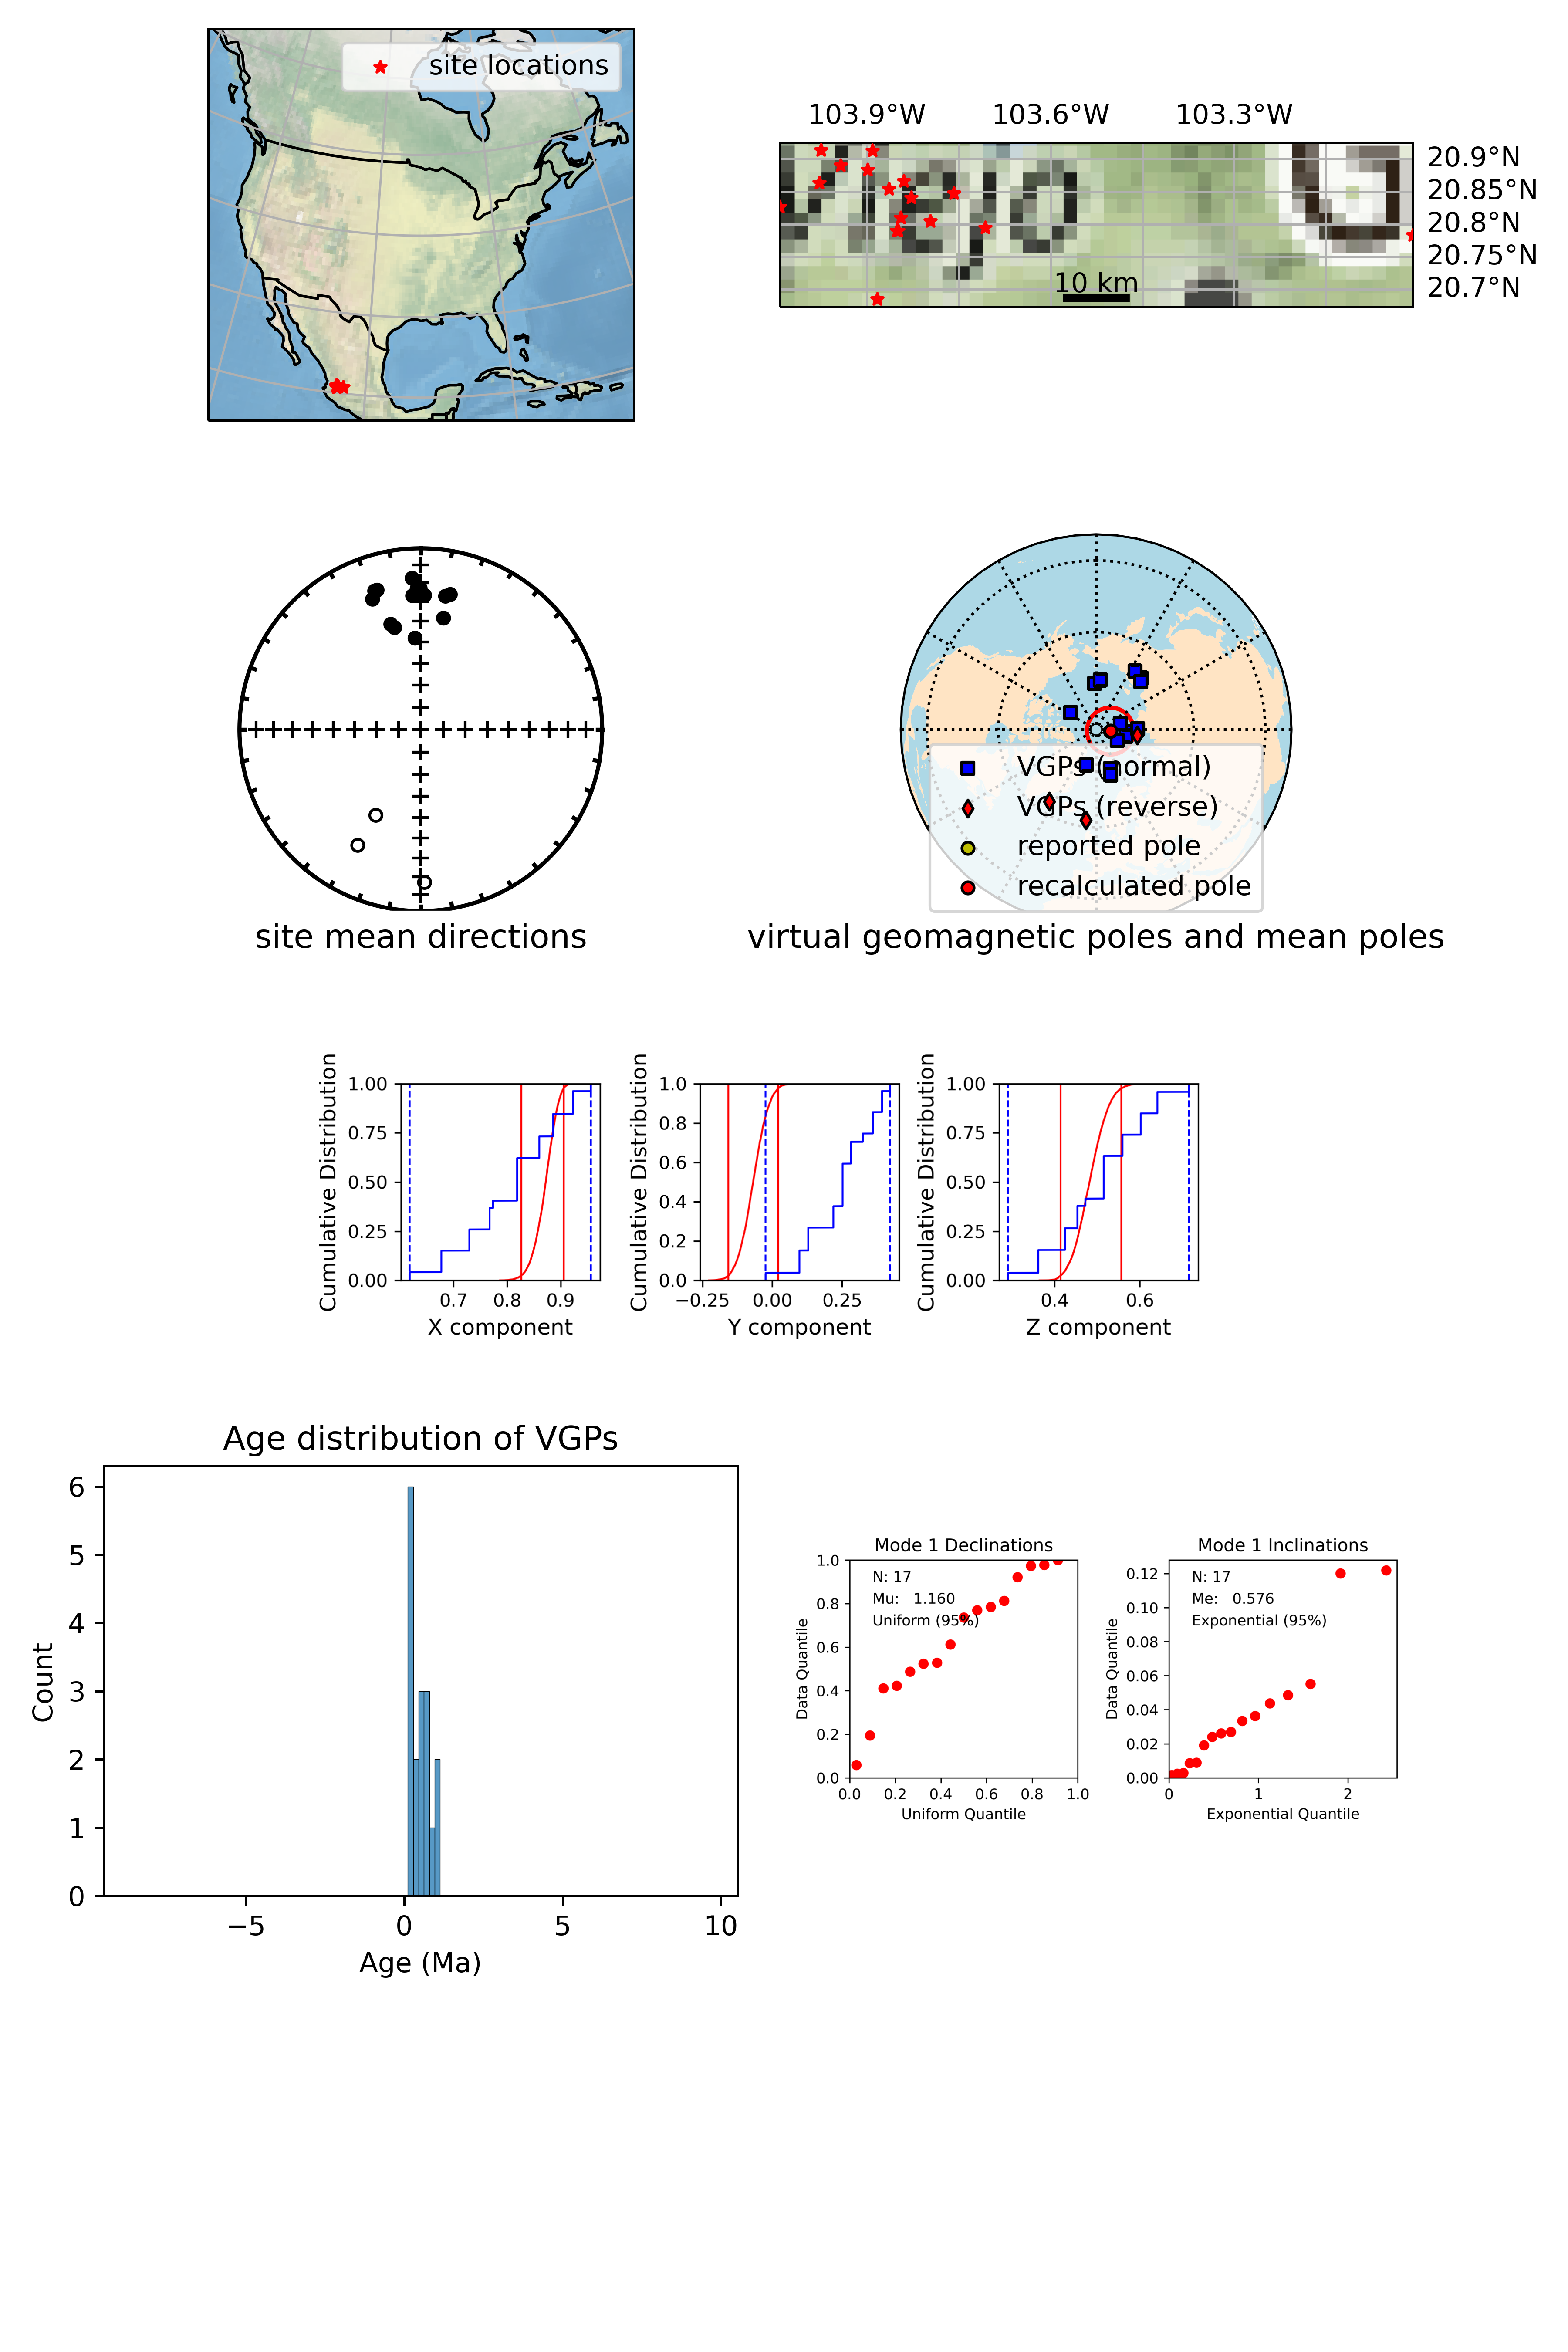
\includegraphics[width=5 in]{./0/1/pole_summary.png}
\caption{Summary of data from locality 0 (Tequila volcanic field) pole 1 (Ceja et al. (2006)).}
\end{figure}

\section{Coso Range volcanics}
\subsection{Pole 1}
\begin{tabular}{lllll}
\toprule
{} &   N &  Plat &   Plon &  A95 \\
\midrule
Reported mean pole                                 &  33 &  88.0 &  265.5 &  5.0 \\
Mean pole (calculated from VGPs)                   &  33 &  87.9 &  270.8 &  5.1 \\
Mean pole (calculated from transformed directions) &  33 &  87.9 &  270.6 &  5.1 \\
\bottomrule
\end{tabular}

\begin{tabular}{ll}
\toprule
{} &                                                          result \\
\midrule
Bootstrap reversal test  &                                                            Pass \\
Parametric reversal test &  Pass (angle 3.1º below 11.5º critical angle); C classification \\
Bayesian reversal test   &                                   Common mean: positive support \\
Fisher Q-Q test          &                             Consistent with Fisher distribution \\
\bottomrule
\end{tabular}

\begin{figure}[H]
\centering
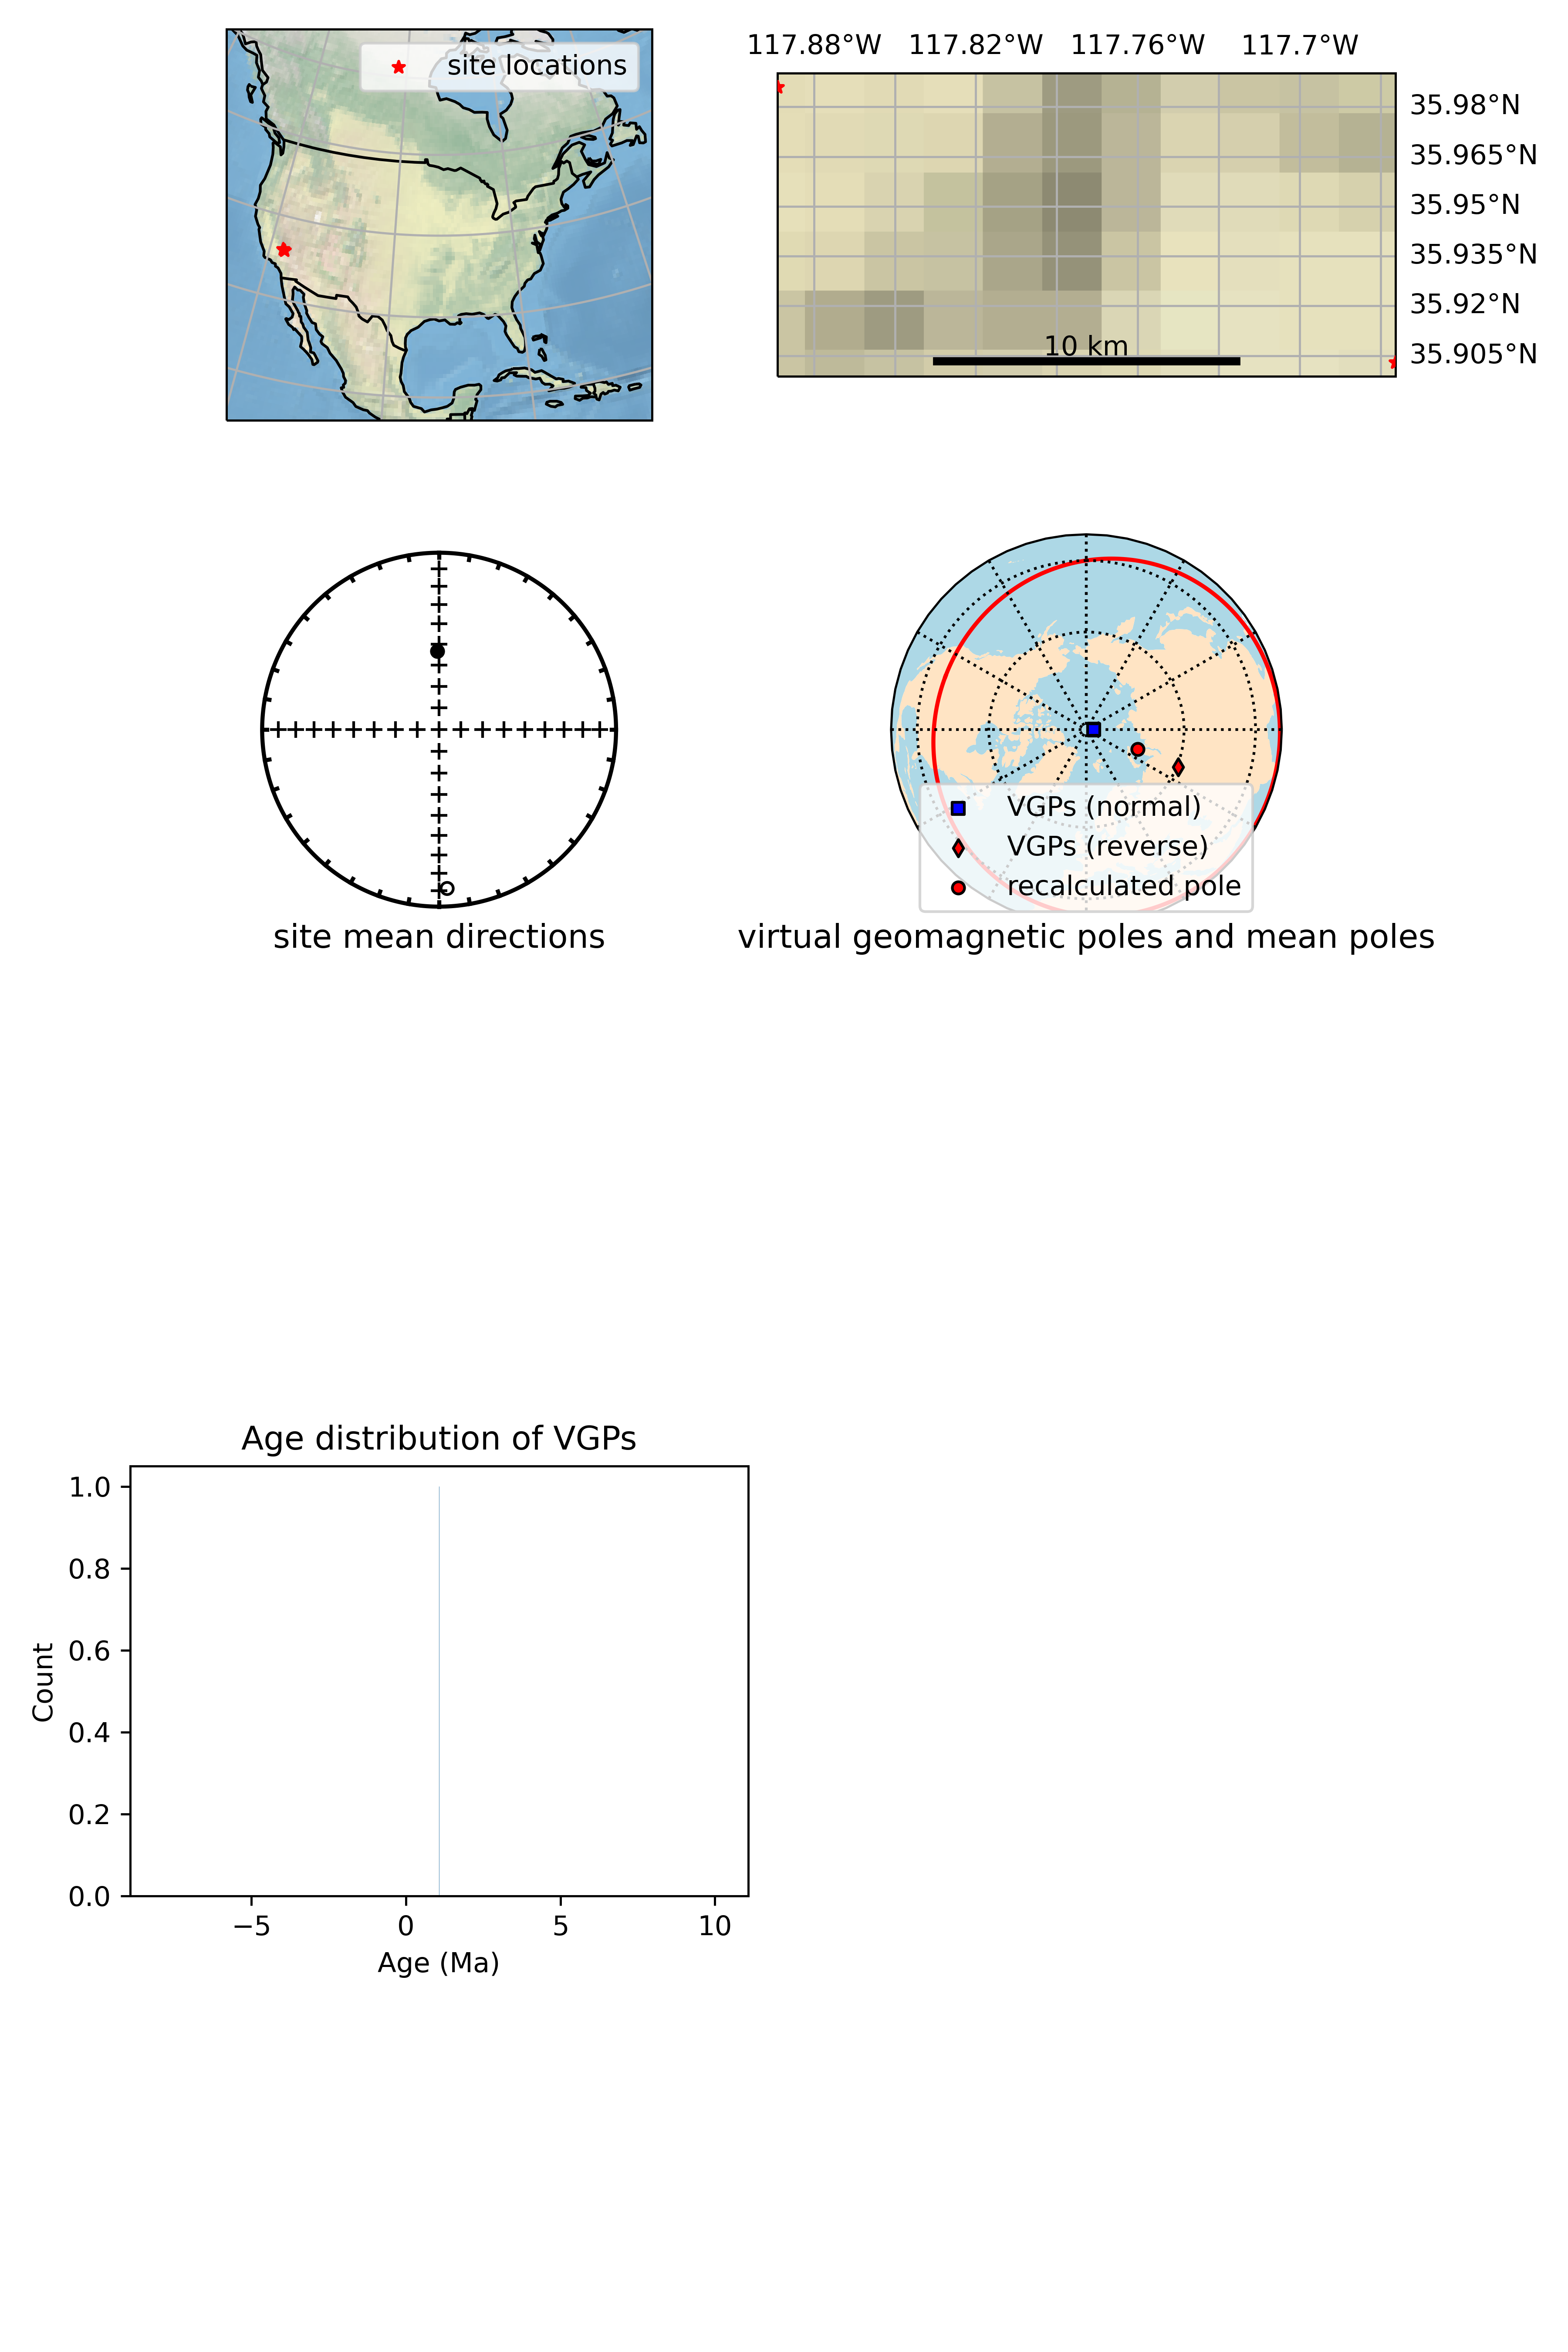
\includegraphics[width=5 in]{./1/1/pole_summary.png}
\caption{Summary of data from locality 1 (Coso Range volcanics) pole 1 (Mankinen and Gromme (1982)).}
\end{figure}

\section{Eastern Alkaline Province}
\subsection{Pole 1}
\begin{tabular}{lllll}
\toprule
{} &   N &  Plat &   Plon &  A95 \\
\midrule
Reported mean pole                                 &  33 &  88.0 &  265.5 &  5.0 \\
Mean pole (calculated from VGPs)                   &  33 &  87.9 &  270.8 &  5.1 \\
Mean pole (calculated from transformed directions) &  33 &  87.9 &  270.6 &  5.1 \\
\bottomrule
\end{tabular}

\begin{tabular}{ll}
\toprule
{} &                                                          result \\
\midrule
Bootstrap reversal test  &                                                            Pass \\
Parametric reversal test &  Pass (angle 3.1º below 11.5º critical angle); C classification \\
Bayesian reversal test   &                                   Common mean: positive support \\
Fisher Q-Q test          &                             Consistent with Fisher distribution \\
\bottomrule
\end{tabular}

\begin{figure}[H]
\centering
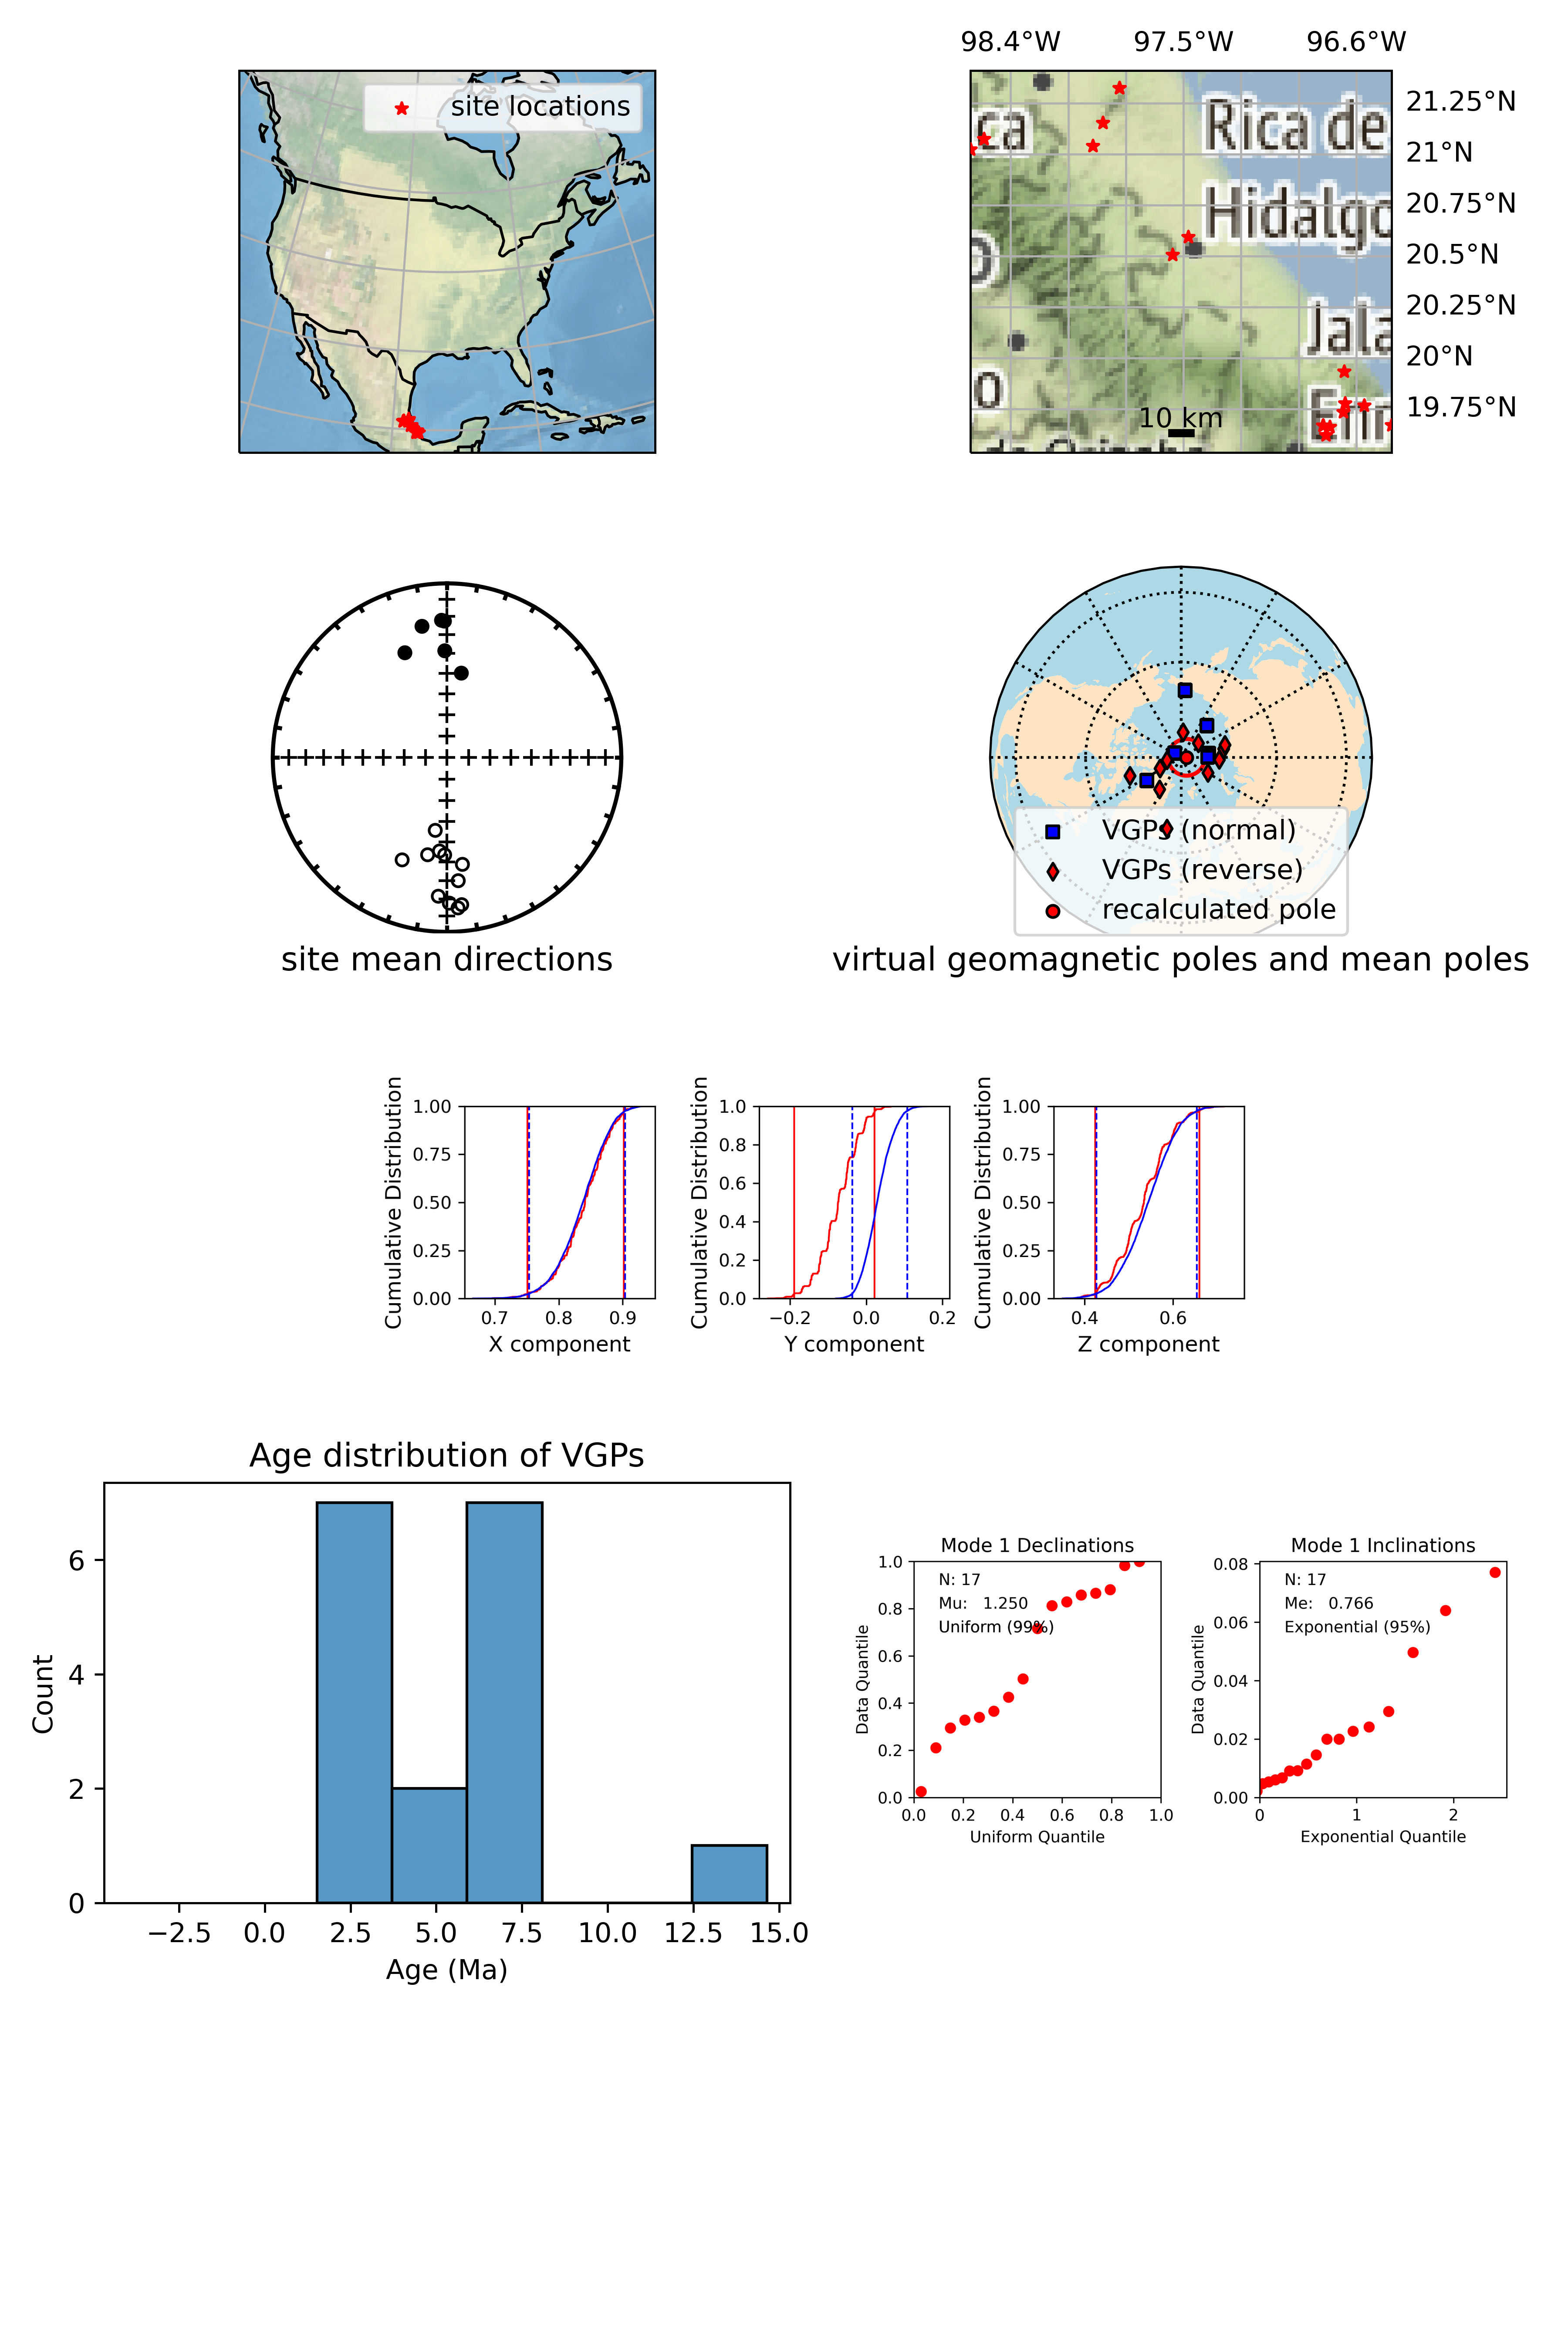
\includegraphics[width=5 in]{./2/1/pole_summary.png}
\caption{Summary of data from locality 2 (Eastern Alkaline Province) pole 1 (Goguitchaichvili et al. (2007)).}
\end{figure}

\section{SW USA composite}
\subsection{Pole 1}
\begin{tabular}{lllll}
\toprule
{} &   N &  Plat &   Plon &  A95 \\
\midrule
Reported mean pole                                 &  33 &  88.0 &  265.5 &  5.0 \\
Mean pole (calculated from VGPs)                   &  33 &  87.9 &  270.8 &  5.1 \\
Mean pole (calculated from transformed directions) &  33 &  87.9 &  270.6 &  5.1 \\
\bottomrule
\end{tabular}

\begin{tabular}{ll}
\toprule
{} &                                                          result \\
\midrule
Bootstrap reversal test  &                                                            Pass \\
Parametric reversal test &  Pass (angle 3.1º below 11.5º critical angle); C classification \\
Bayesian reversal test   &                                   Common mean: positive support \\
Fisher Q-Q test          &                             Consistent with Fisher distribution \\
\bottomrule
\end{tabular}

\begin{figure}[H]
\centering
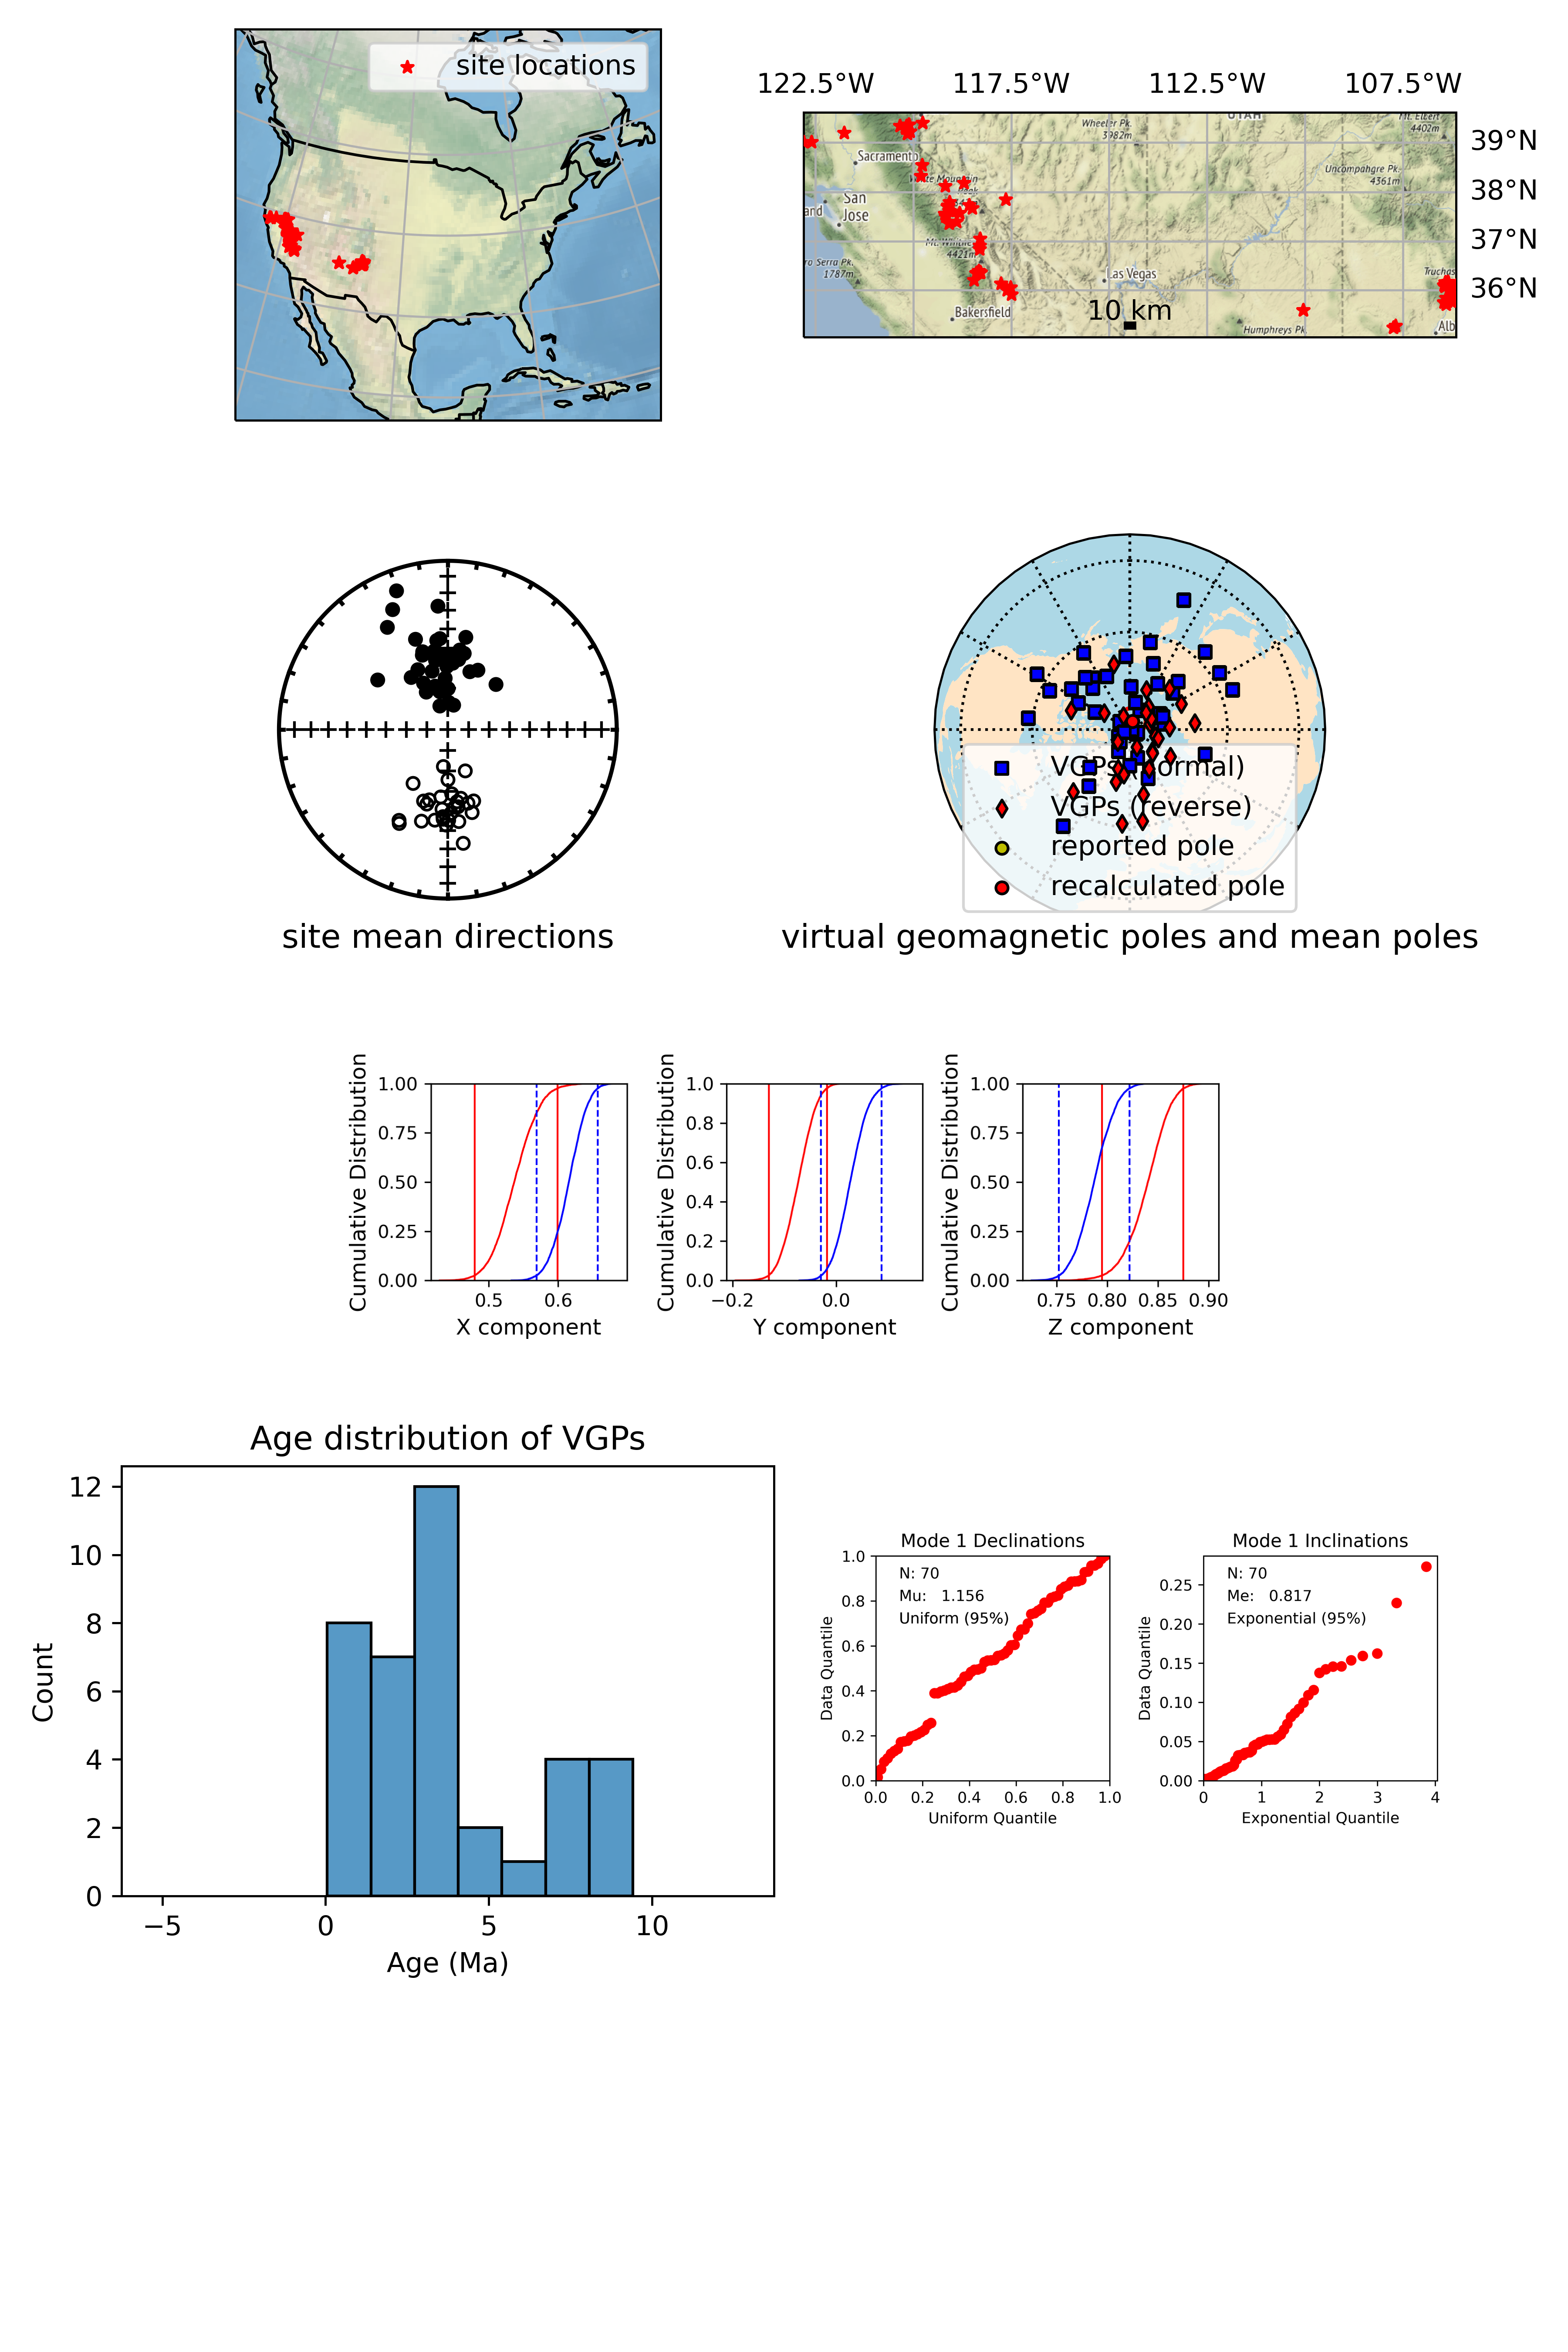
\includegraphics[width=5 in]{./3/1/pole_summary.png}
\caption{Summary of data from locality 3 (SW USA composite) pole 1 (Mankinen (2008)).}
\end{figure}

\section{N Montana intrusions}
\subsection{Pole 1}
\begin{tabular}{lllll}
\toprule
{} &   N &  Plat &   Plon &  A95 \\
\midrule
Reported mean pole                                 &  33 &  88.0 &  265.5 &  5.0 \\
Mean pole (calculated from VGPs)                   &  33 &  87.9 &  270.8 &  5.1 \\
Mean pole (calculated from transformed directions) &  33 &  87.9 &  270.6 &  5.1 \\
\bottomrule
\end{tabular}

\begin{tabular}{ll}
\toprule
{} &                                                          result \\
\midrule
Bootstrap reversal test  &                                                            Pass \\
Parametric reversal test &  Pass (angle 3.1º below 11.5º critical angle); C classification \\
Bayesian reversal test   &                                   Common mean: positive support \\
Fisher Q-Q test          &                             Consistent with Fisher distribution \\
\bottomrule
\end{tabular}

\begin{figure}[H]
\centering
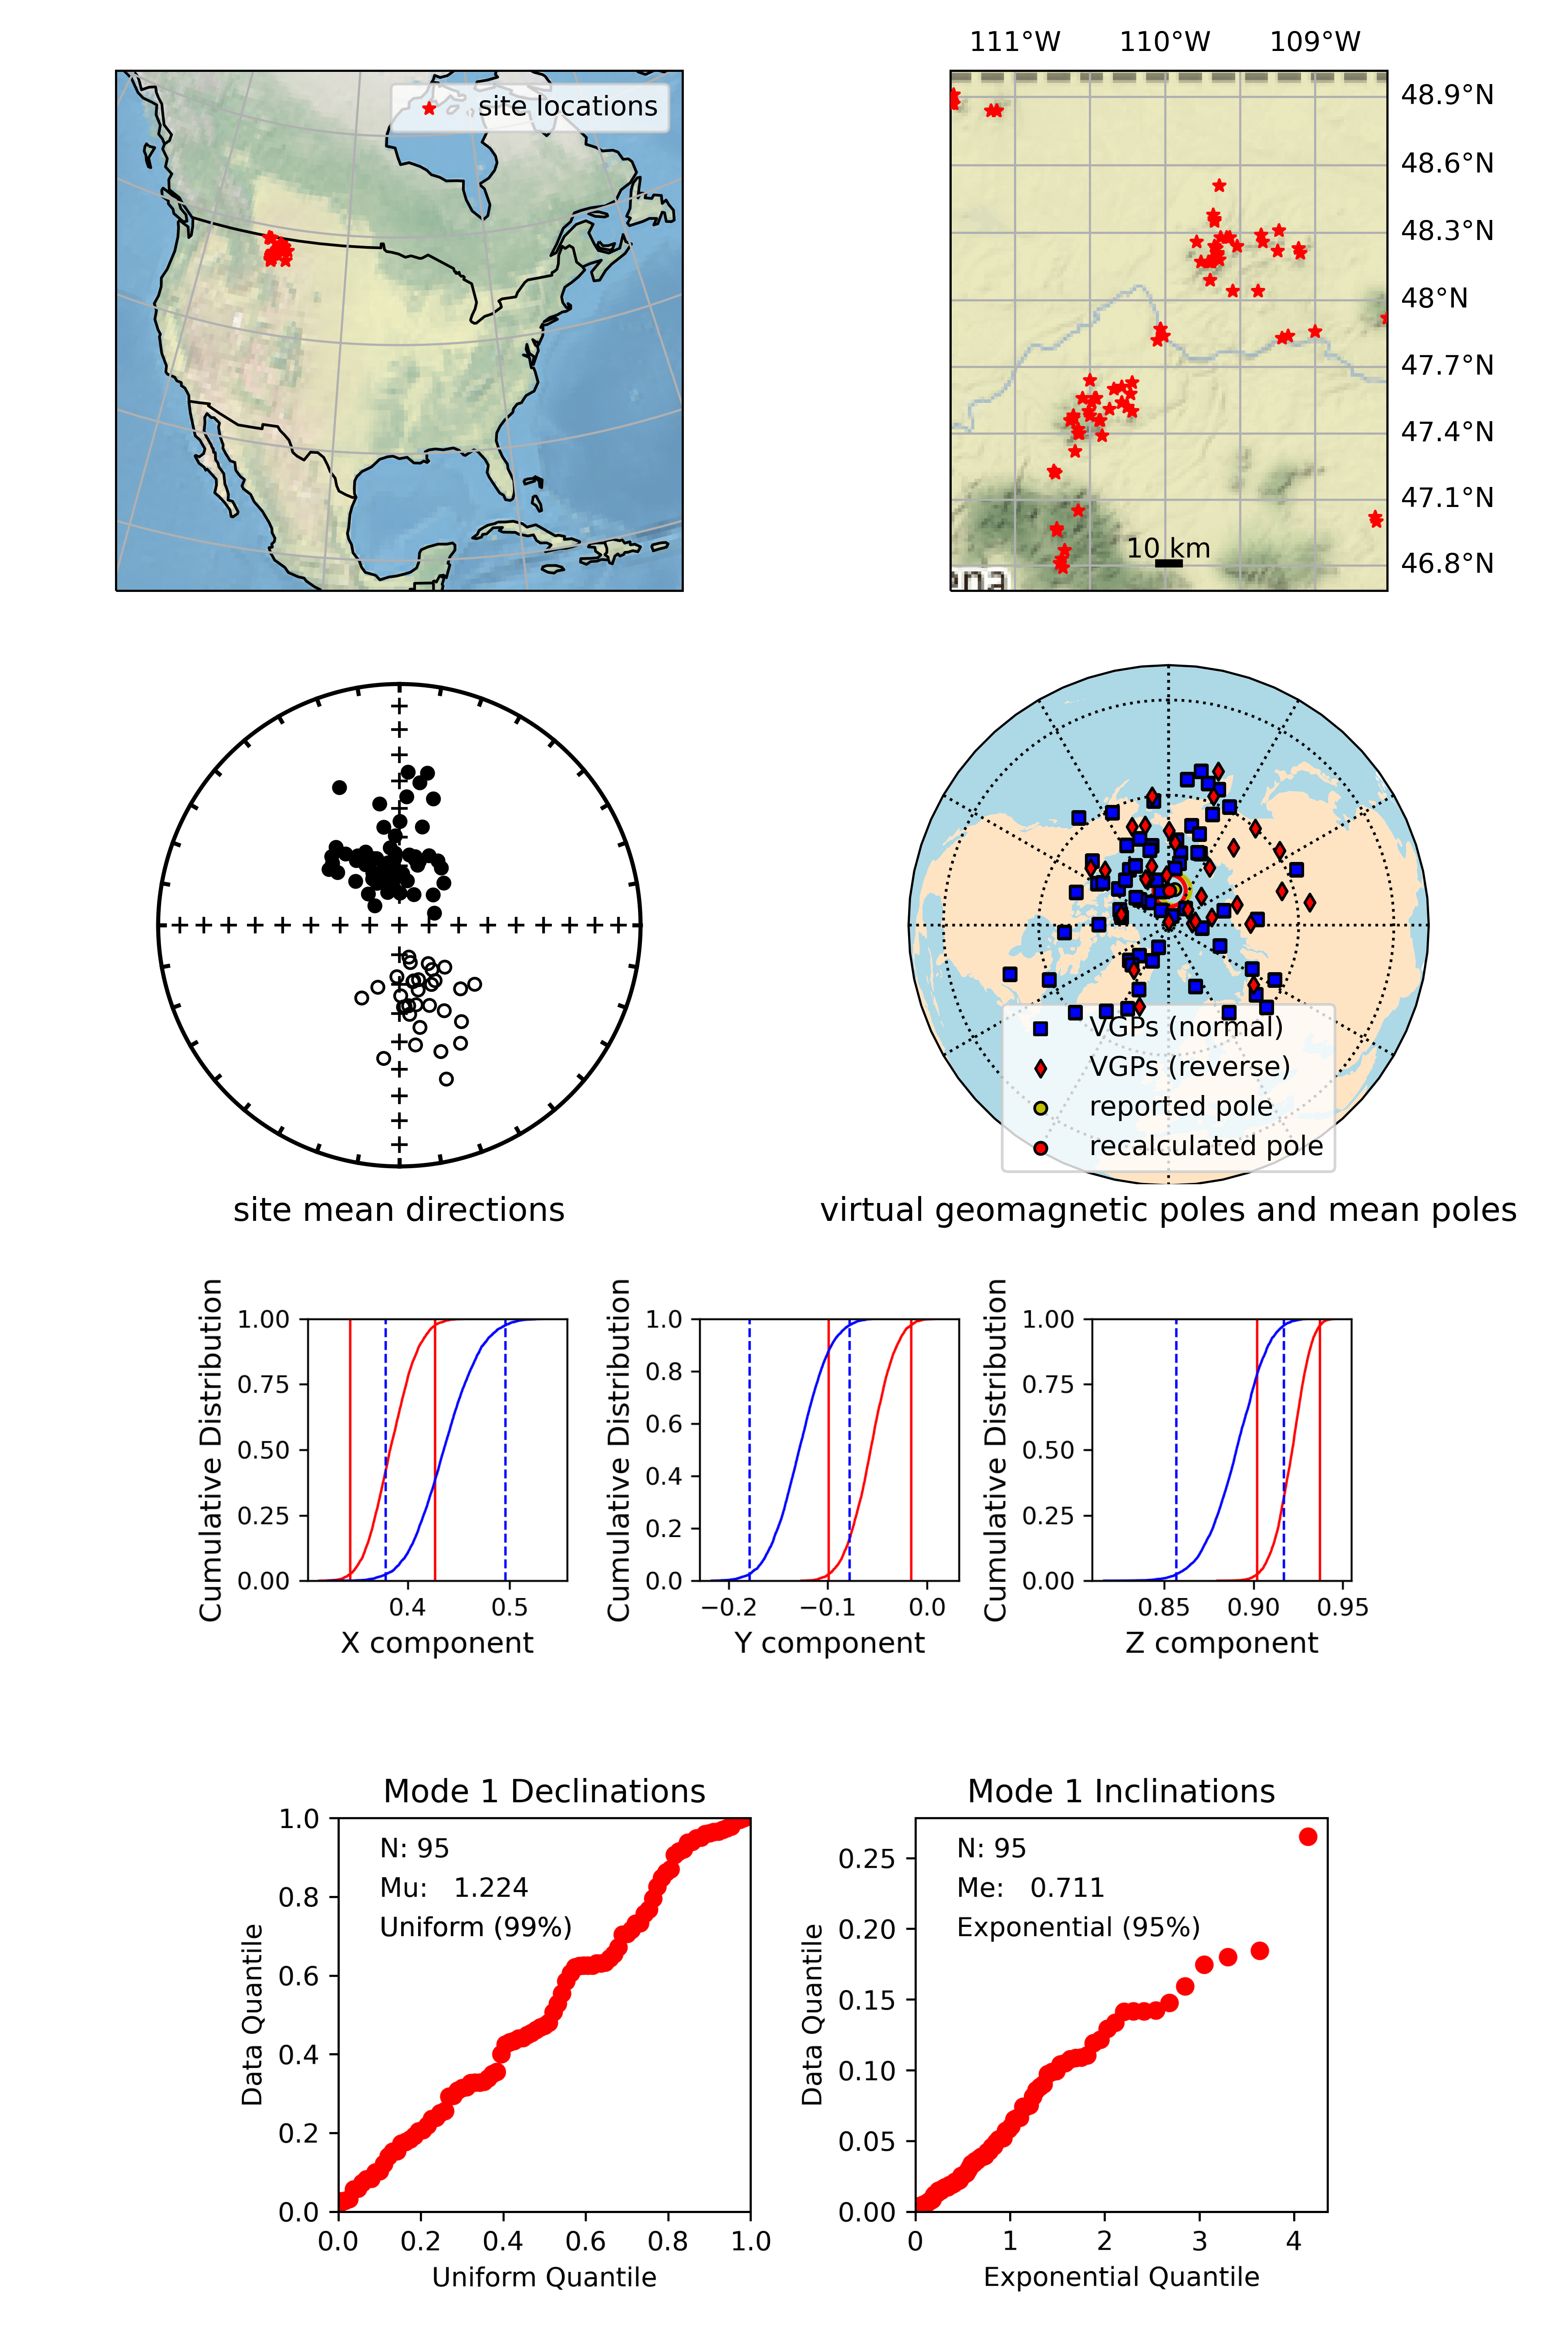
\includegraphics[width=5 in]{./4/1/pole_summary.png}
\caption{Summary of data from locality 4 (N Montana intrusions) pole 1 (Diehl et al. (1983)).}
\end{figure}

\section{Long Valley Caldera volcanics}
\subsection{Pole 1}
\begin{tabular}{lllll}
\toprule
{} &   N &  Plat &   Plon &  A95 \\
\midrule
Reported mean pole                                 &  33 &  88.0 &  265.5 &  5.0 \\
Mean pole (calculated from VGPs)                   &  33 &  87.9 &  270.8 &  5.1 \\
Mean pole (calculated from transformed directions) &  33 &  87.9 &  270.6 &  5.1 \\
\bottomrule
\end{tabular}

\begin{tabular}{ll}
\toprule
{} &                                                          result \\
\midrule
Bootstrap reversal test  &                                                            Pass \\
Parametric reversal test &  Pass (angle 3.1º below 11.5º critical angle); C classification \\
Bayesian reversal test   &                                   Common mean: positive support \\
Fisher Q-Q test          &                             Consistent with Fisher distribution \\
\bottomrule
\end{tabular}

\begin{figure}[H]
\centering
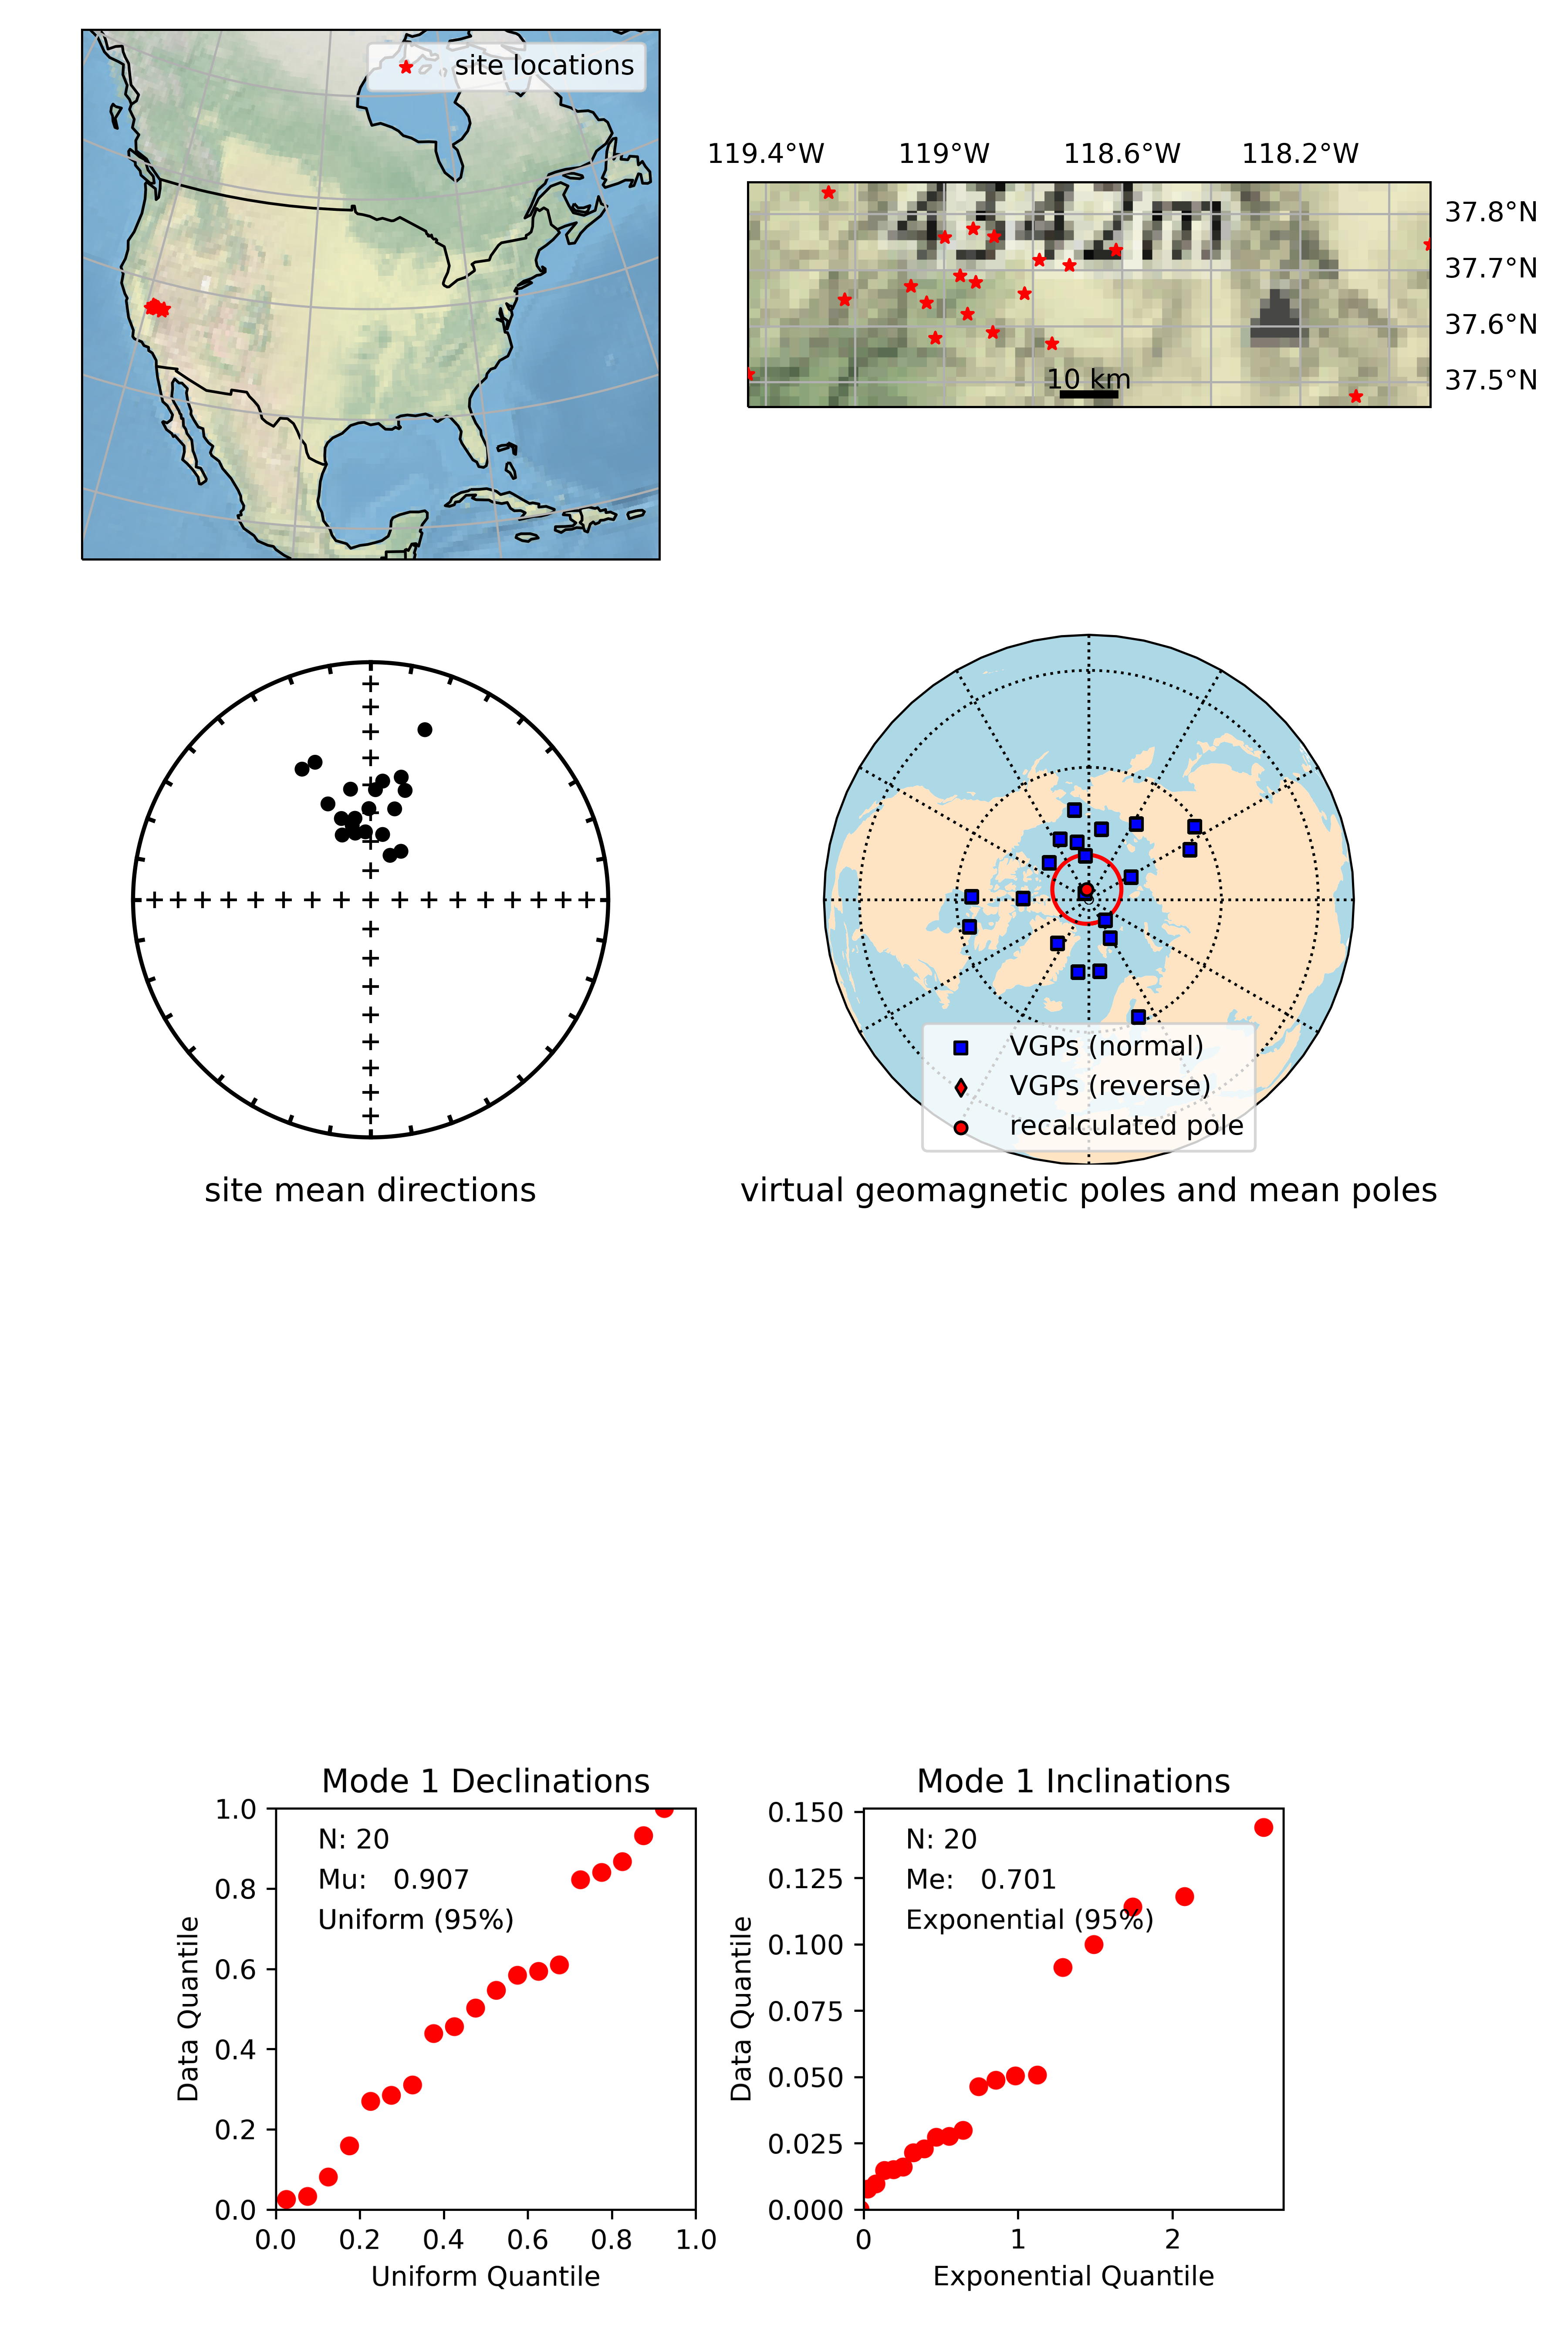
\includegraphics[width=5 in]{./5/1/pole_summary.png}
\caption{Summary of data from locality 5 (Long Valley Caldera volcanics) pole 1 (Mankinen et al. (1986)).}
\end{figure}

\section{Robinson Antincline intrusions}
\subsection{Pole 1}
\begin{tabular}{lllll}
\toprule
{} &   N &  Plat &   Plon &  A95 \\
\midrule
Reported mean pole                                 &  33 &  88.0 &  265.5 &  5.0 \\
Mean pole (calculated from VGPs)                   &  33 &  87.9 &  270.8 &  5.1 \\
Mean pole (calculated from transformed directions) &  33 &  87.9 &  270.6 &  5.1 \\
\bottomrule
\end{tabular}

\begin{tabular}{ll}
\toprule
{} &                                                          result \\
\midrule
Bootstrap reversal test  &                                                            Pass \\
Parametric reversal test &  Pass (angle 3.1º below 11.5º critical angle); C classification \\
Bayesian reversal test   &                                   Common mean: positive support \\
Fisher Q-Q test          &                             Consistent with Fisher distribution \\
\bottomrule
\end{tabular}

\begin{figure}[H]
\centering
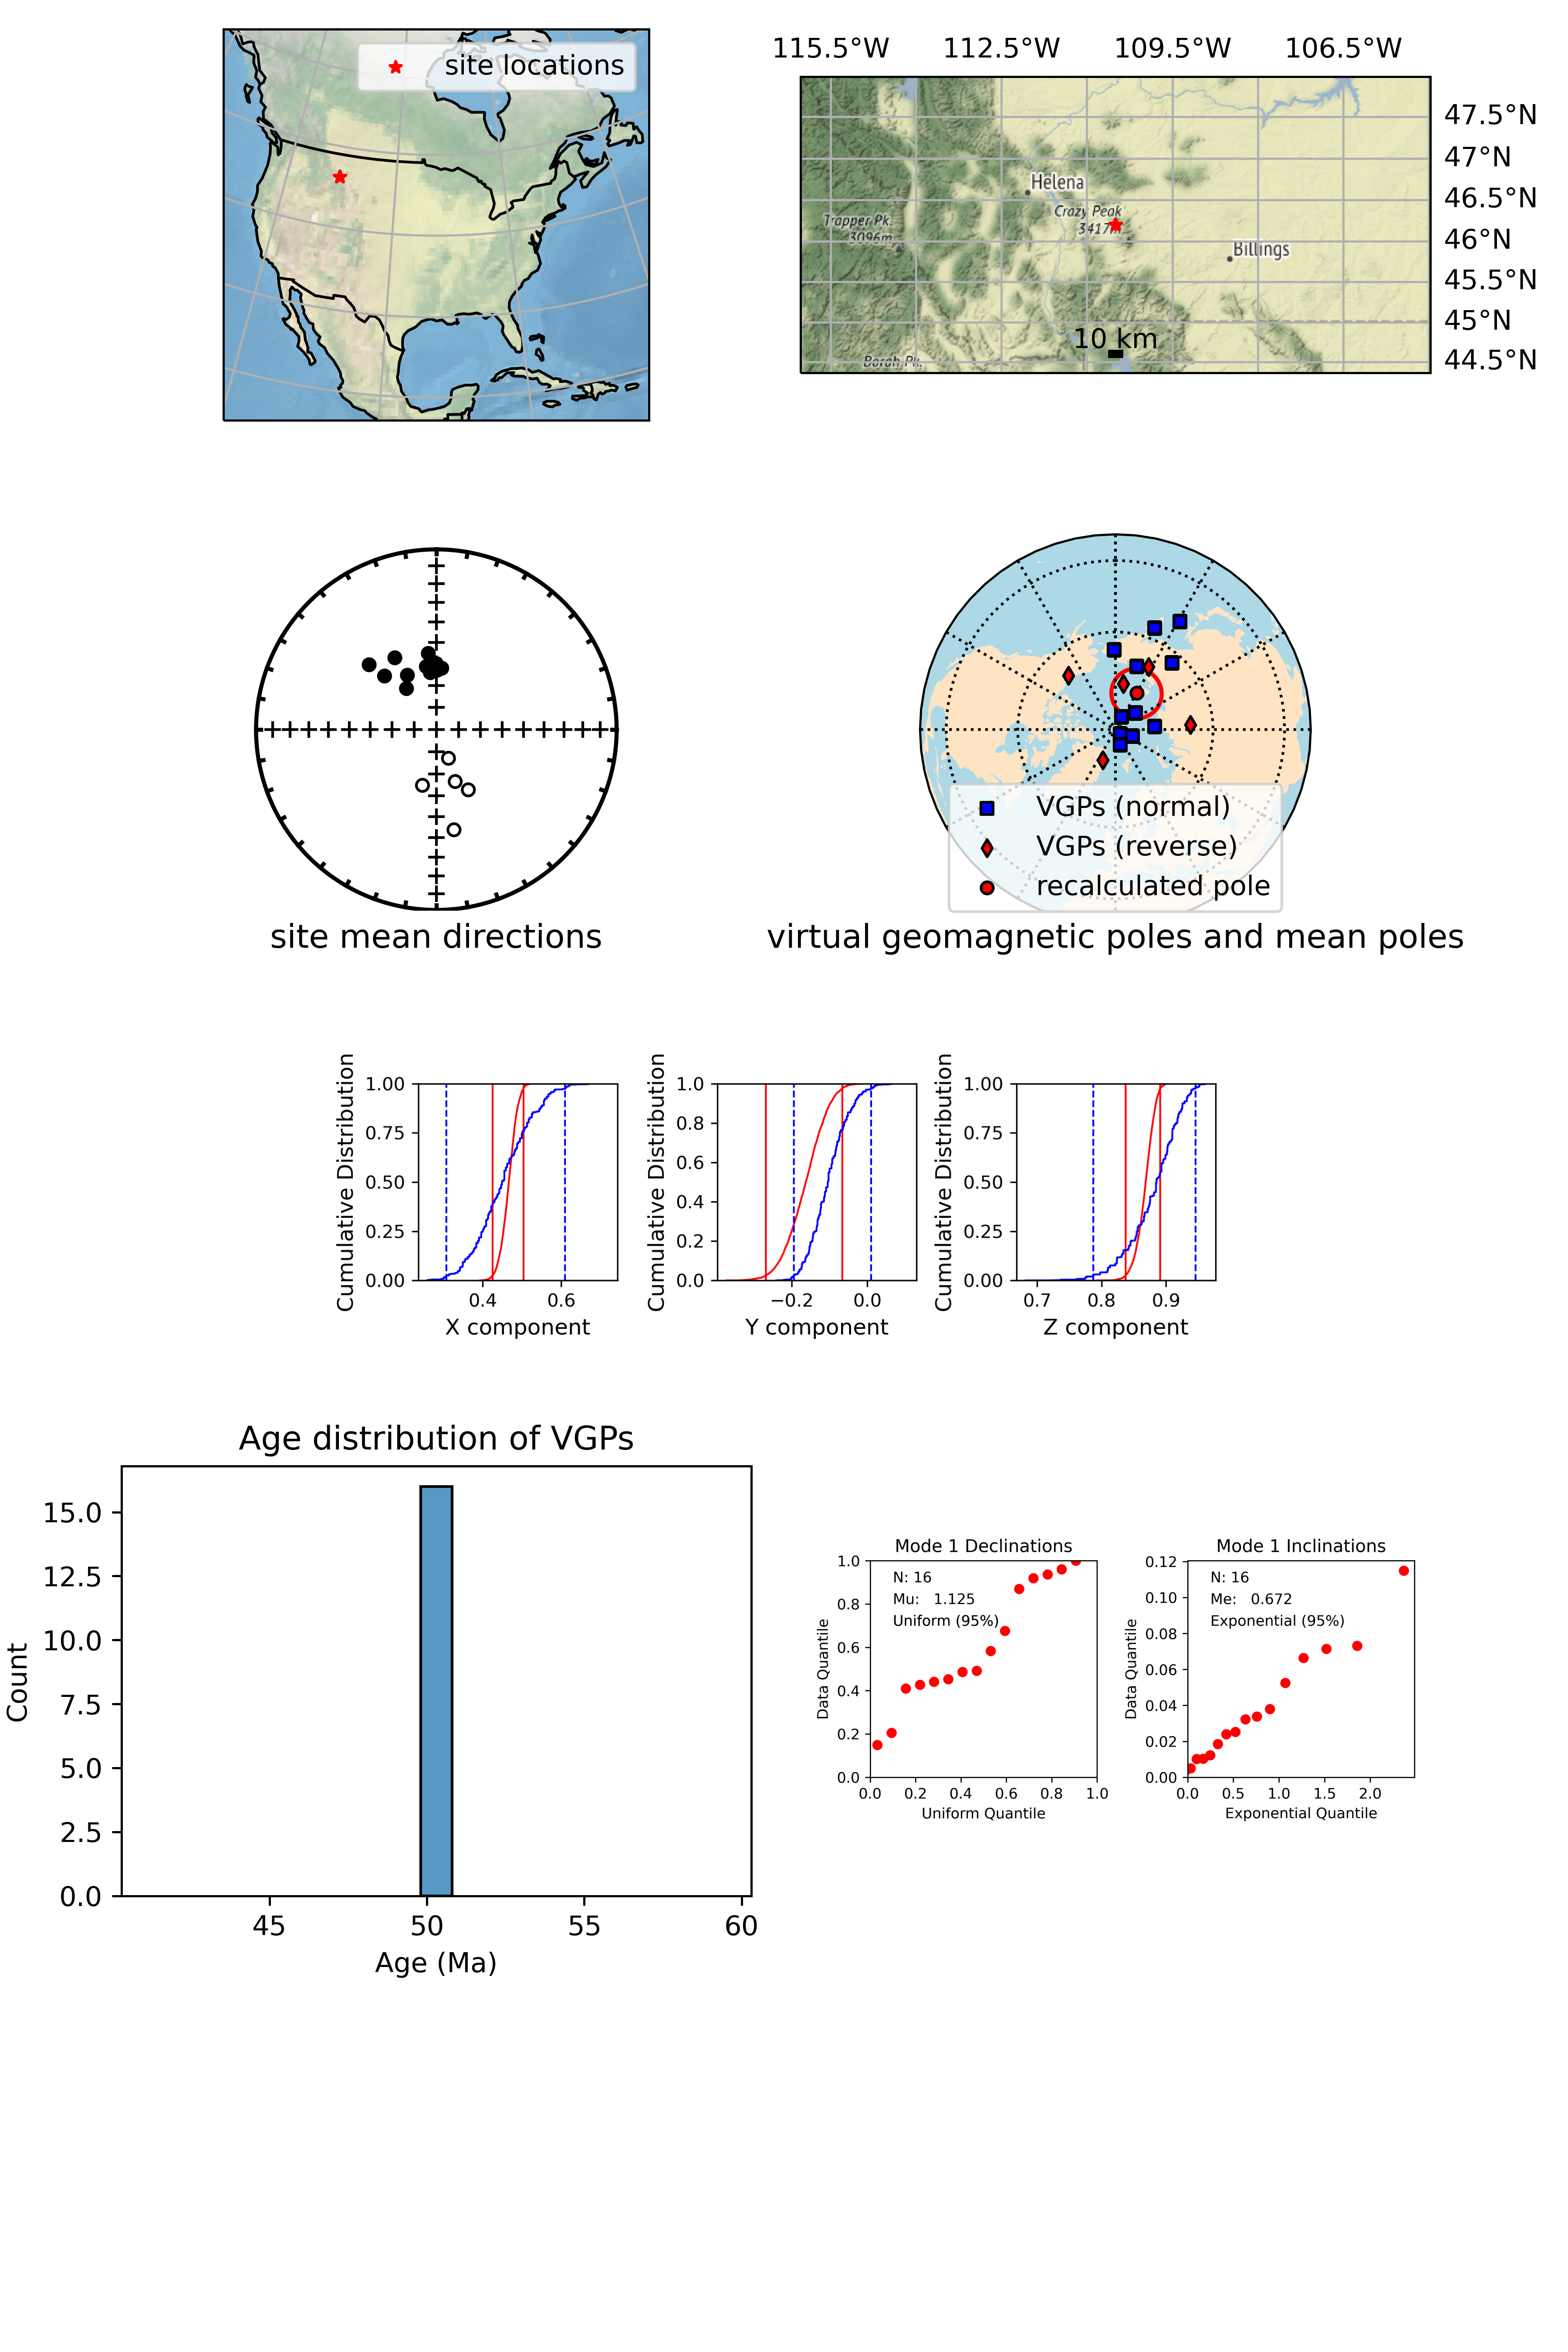
\includegraphics[width=5 in]{./6/1/pole_summary.png}
\caption{Summary of data from locality 6 (Robinson Antincline intrusions) pole 1 (Recalculated after data provided in Harlan et al. (1988).).}
\end{figure}

\section{Central Mexico Plio-Pleistocene}
\subsection{Pole 1}
\begin{tabular}{lllll}
\toprule
{} &   N &  Plat &   Plon &  A95 \\
\midrule
Reported mean pole                                 &  33 &  88.0 &  265.5 &  5.0 \\
Mean pole (calculated from VGPs)                   &  33 &  87.9 &  270.8 &  5.1 \\
Mean pole (calculated from transformed directions) &  33 &  87.9 &  270.6 &  5.1 \\
\bottomrule
\end{tabular}

\begin{tabular}{ll}
\toprule
{} &                                                          result \\
\midrule
Bootstrap reversal test  &                                                            Pass \\
Parametric reversal test &  Pass (angle 3.1º below 11.5º critical angle); C classification \\
Bayesian reversal test   &                                   Common mean: positive support \\
Fisher Q-Q test          &                             Consistent with Fisher distribution \\
\bottomrule
\end{tabular}

\begin{figure}[H]
\centering
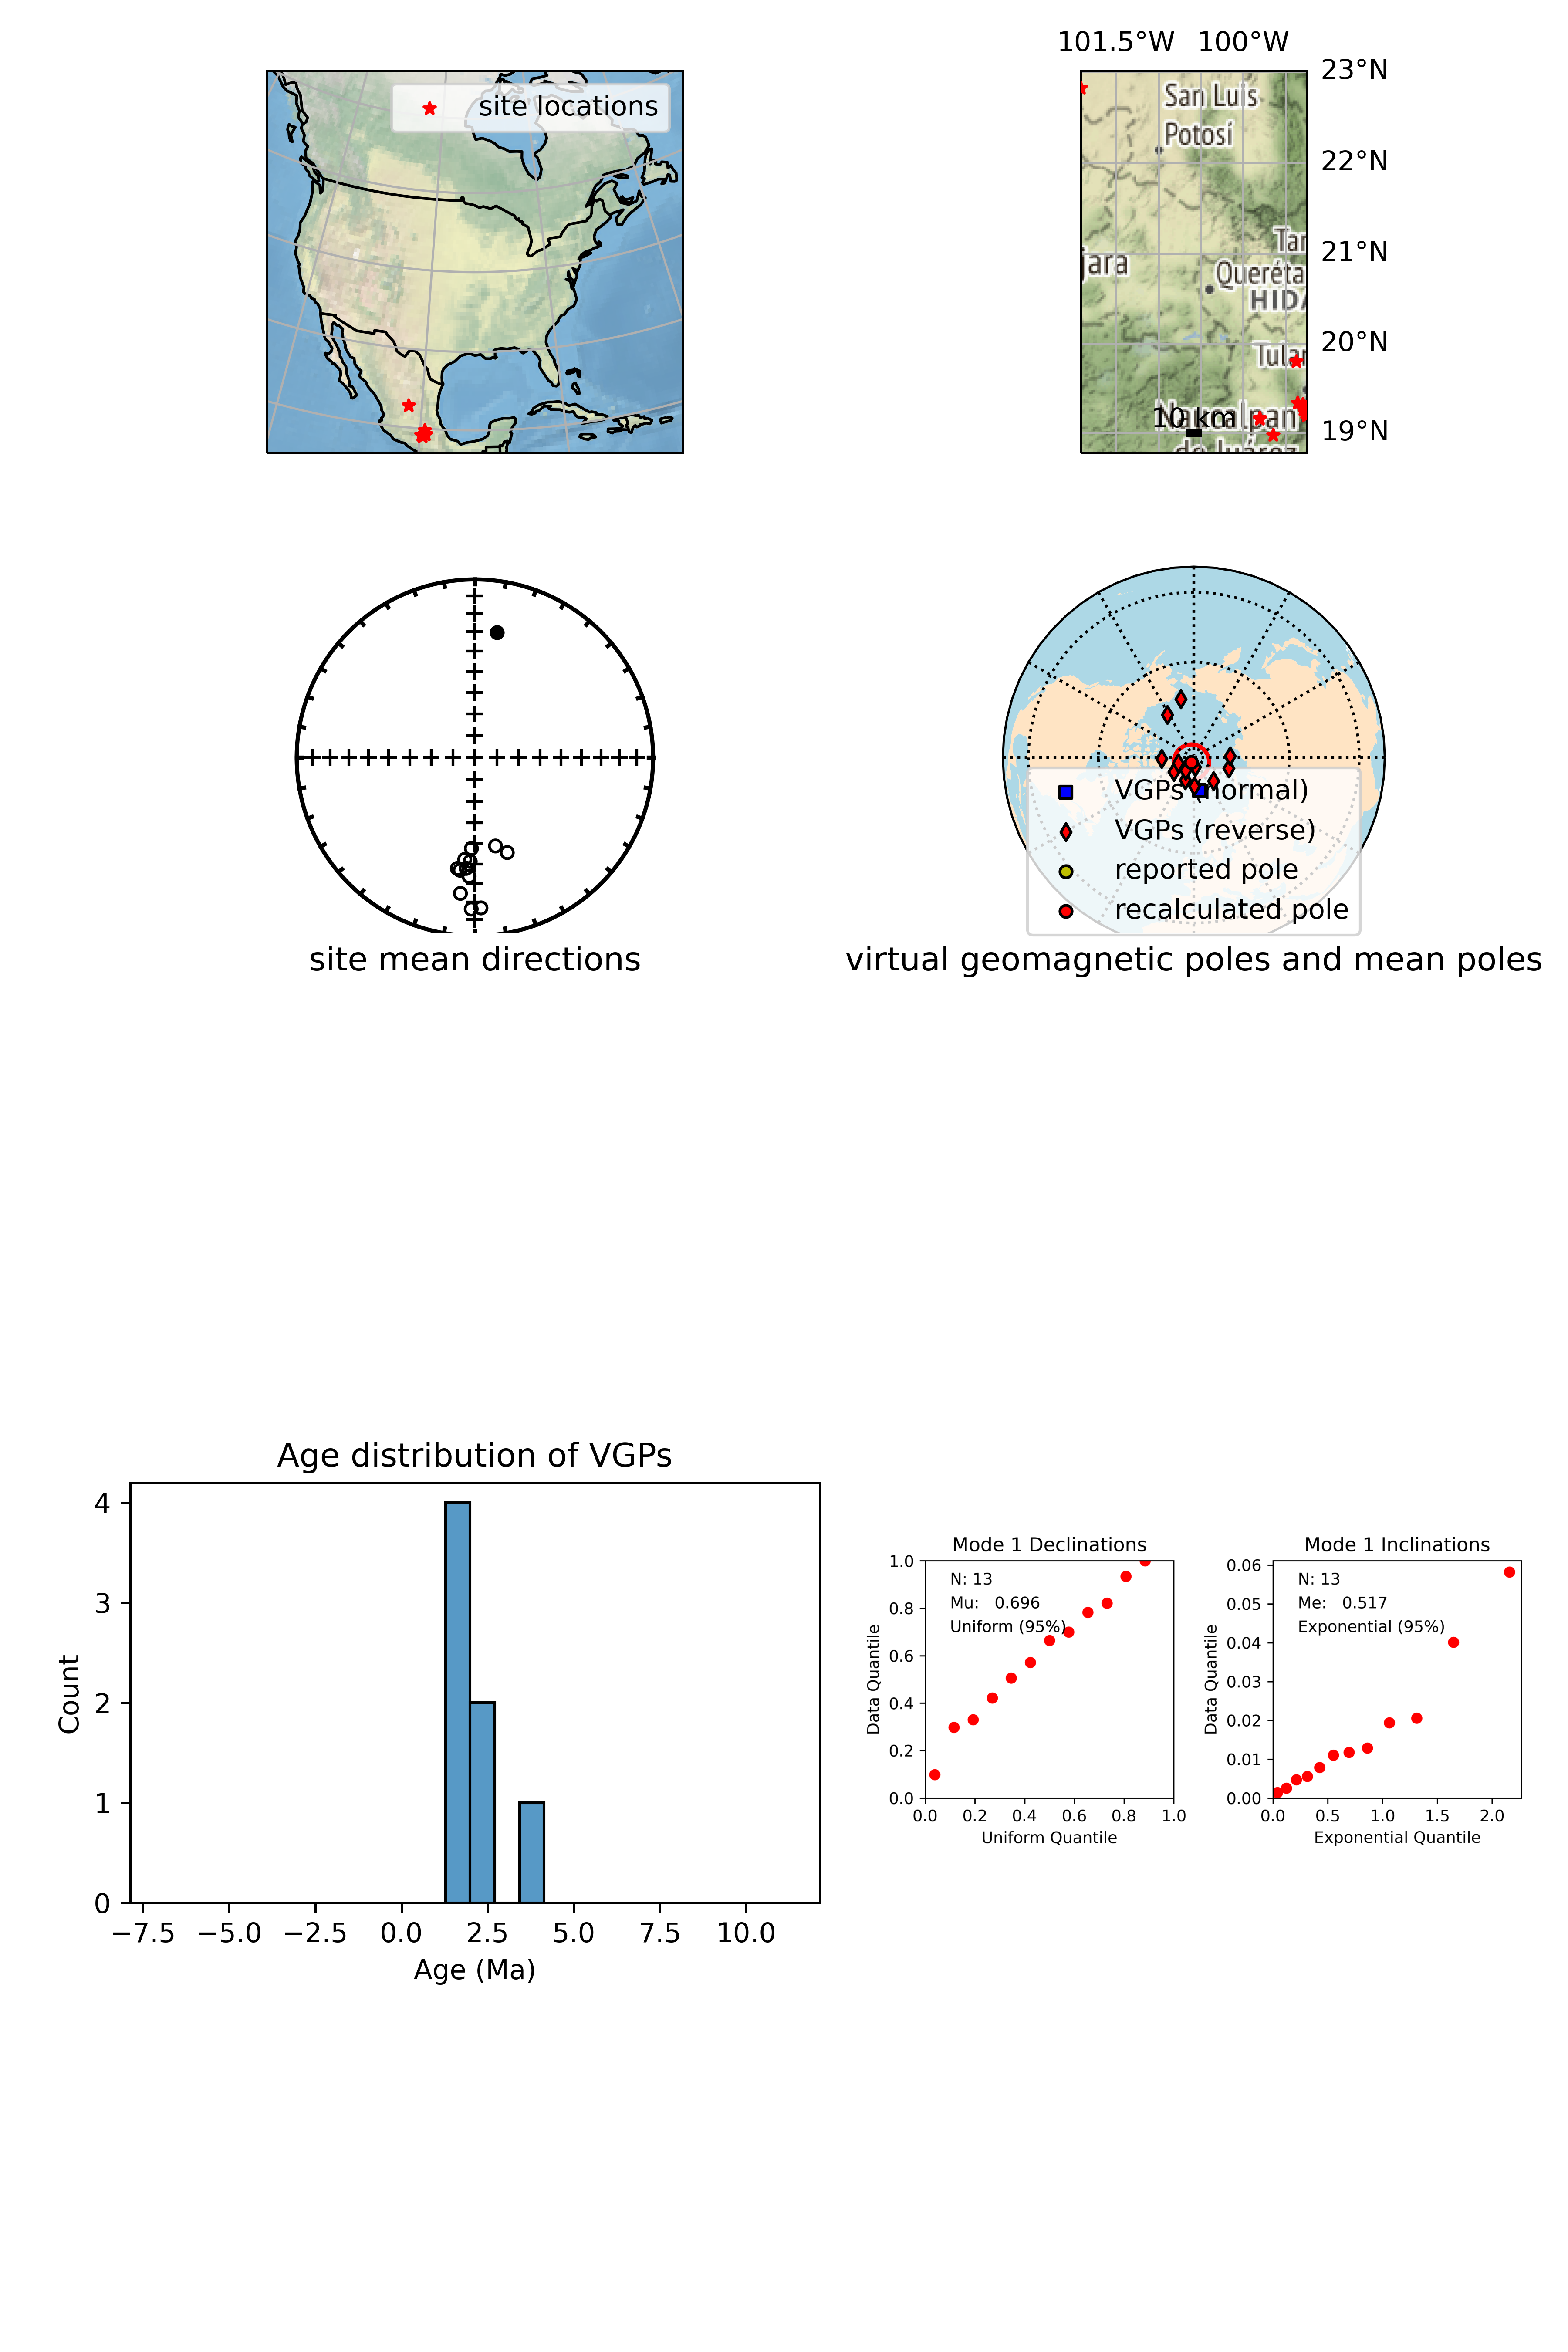
\includegraphics[width=5 in]{./7/1/pole_summary.png}
\caption{Summary of data from locality 7 (Central Mexico Plio-Pleistocene) pole 1 (Mejia et al. (2005)).}
\end{figure}

\section{Rattlesnake Hills volcanics}
\subsection{Pole 1}
\begin{tabular}{lllll}
\toprule
{} &   N &  Plat &   Plon &  A95 \\
\midrule
Reported mean pole                                 &  33 &  88.0 &  265.5 &  5.0 \\
Mean pole (calculated from VGPs)                   &  33 &  87.9 &  270.8 &  5.1 \\
Mean pole (calculated from transformed directions) &  33 &  87.9 &  270.6 &  5.1 \\
\bottomrule
\end{tabular}

\begin{tabular}{ll}
\toprule
{} &                                                          result \\
\midrule
Bootstrap reversal test  &                                                            Pass \\
Parametric reversal test &  Pass (angle 3.1º below 11.5º critical angle); C classification \\
Bayesian reversal test   &                                   Common mean: positive support \\
Fisher Q-Q test          &                             Consistent with Fisher distribution \\
\bottomrule
\end{tabular}

\begin{figure}[H]
\centering
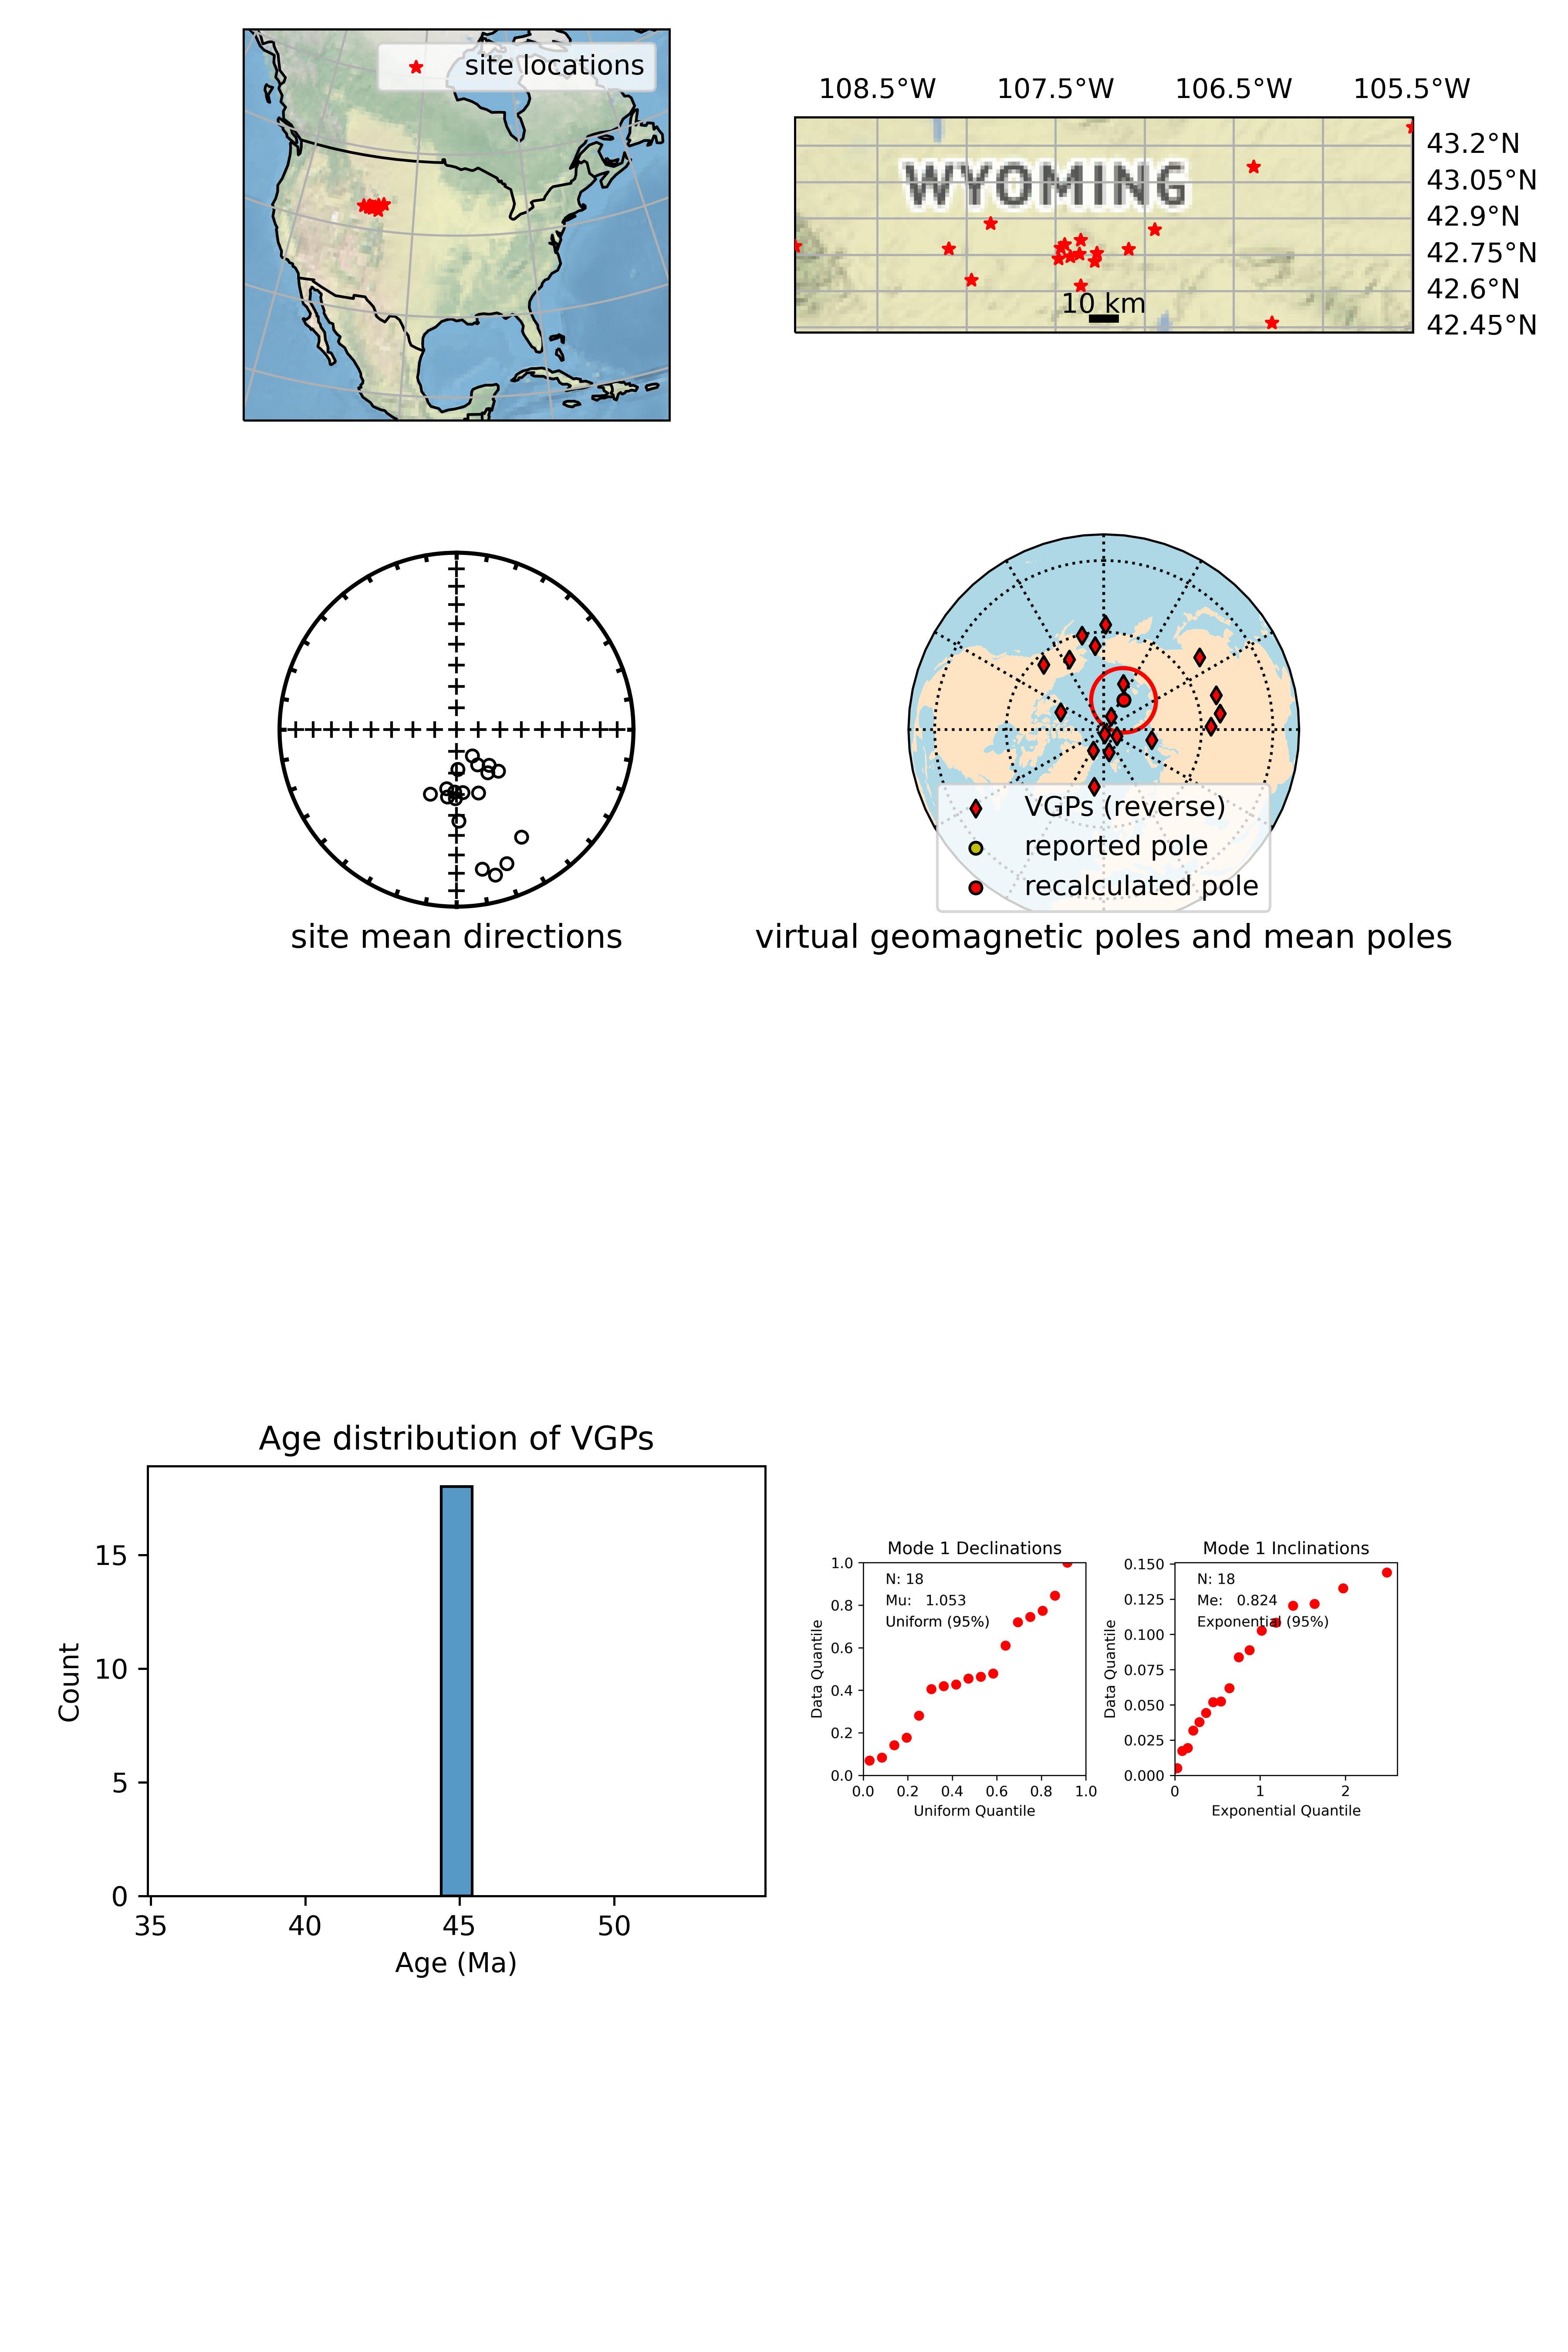
\includegraphics[width=5 in]{./8/1/pole_summary.png}
\caption{Summary of data from locality 8 (Rattlesnake Hills volcanics) pole 1 (Sheriff and Shive (1980)).}
\end{figure}

\section{Ramsay Island lavas}
\subsection{Pole 1}
\begin{tabular}{lllll}
\toprule
{} &   N &  Plat &   Plon &  A95 \\
\midrule
Reported mean pole                                 &  33 &  88.0 &  265.5 &  5.0 \\
Mean pole (calculated from VGPs)                   &  33 &  87.9 &  270.8 &  5.1 \\
Mean pole (calculated from transformed directions) &  33 &  87.9 &  270.6 &  5.1 \\
\bottomrule
\end{tabular}

\begin{tabular}{ll}
\toprule
{} &                                                          result \\
\midrule
Bootstrap reversal test  &                                                            Pass \\
Parametric reversal test &  Pass (angle 3.1º below 11.5º critical angle); C classification \\
Bayesian reversal test   &                                   Common mean: positive support \\
Fisher Q-Q test          &                             Consistent with Fisher distribution \\
\bottomrule
\end{tabular}

\begin{figure}[H]
\centering
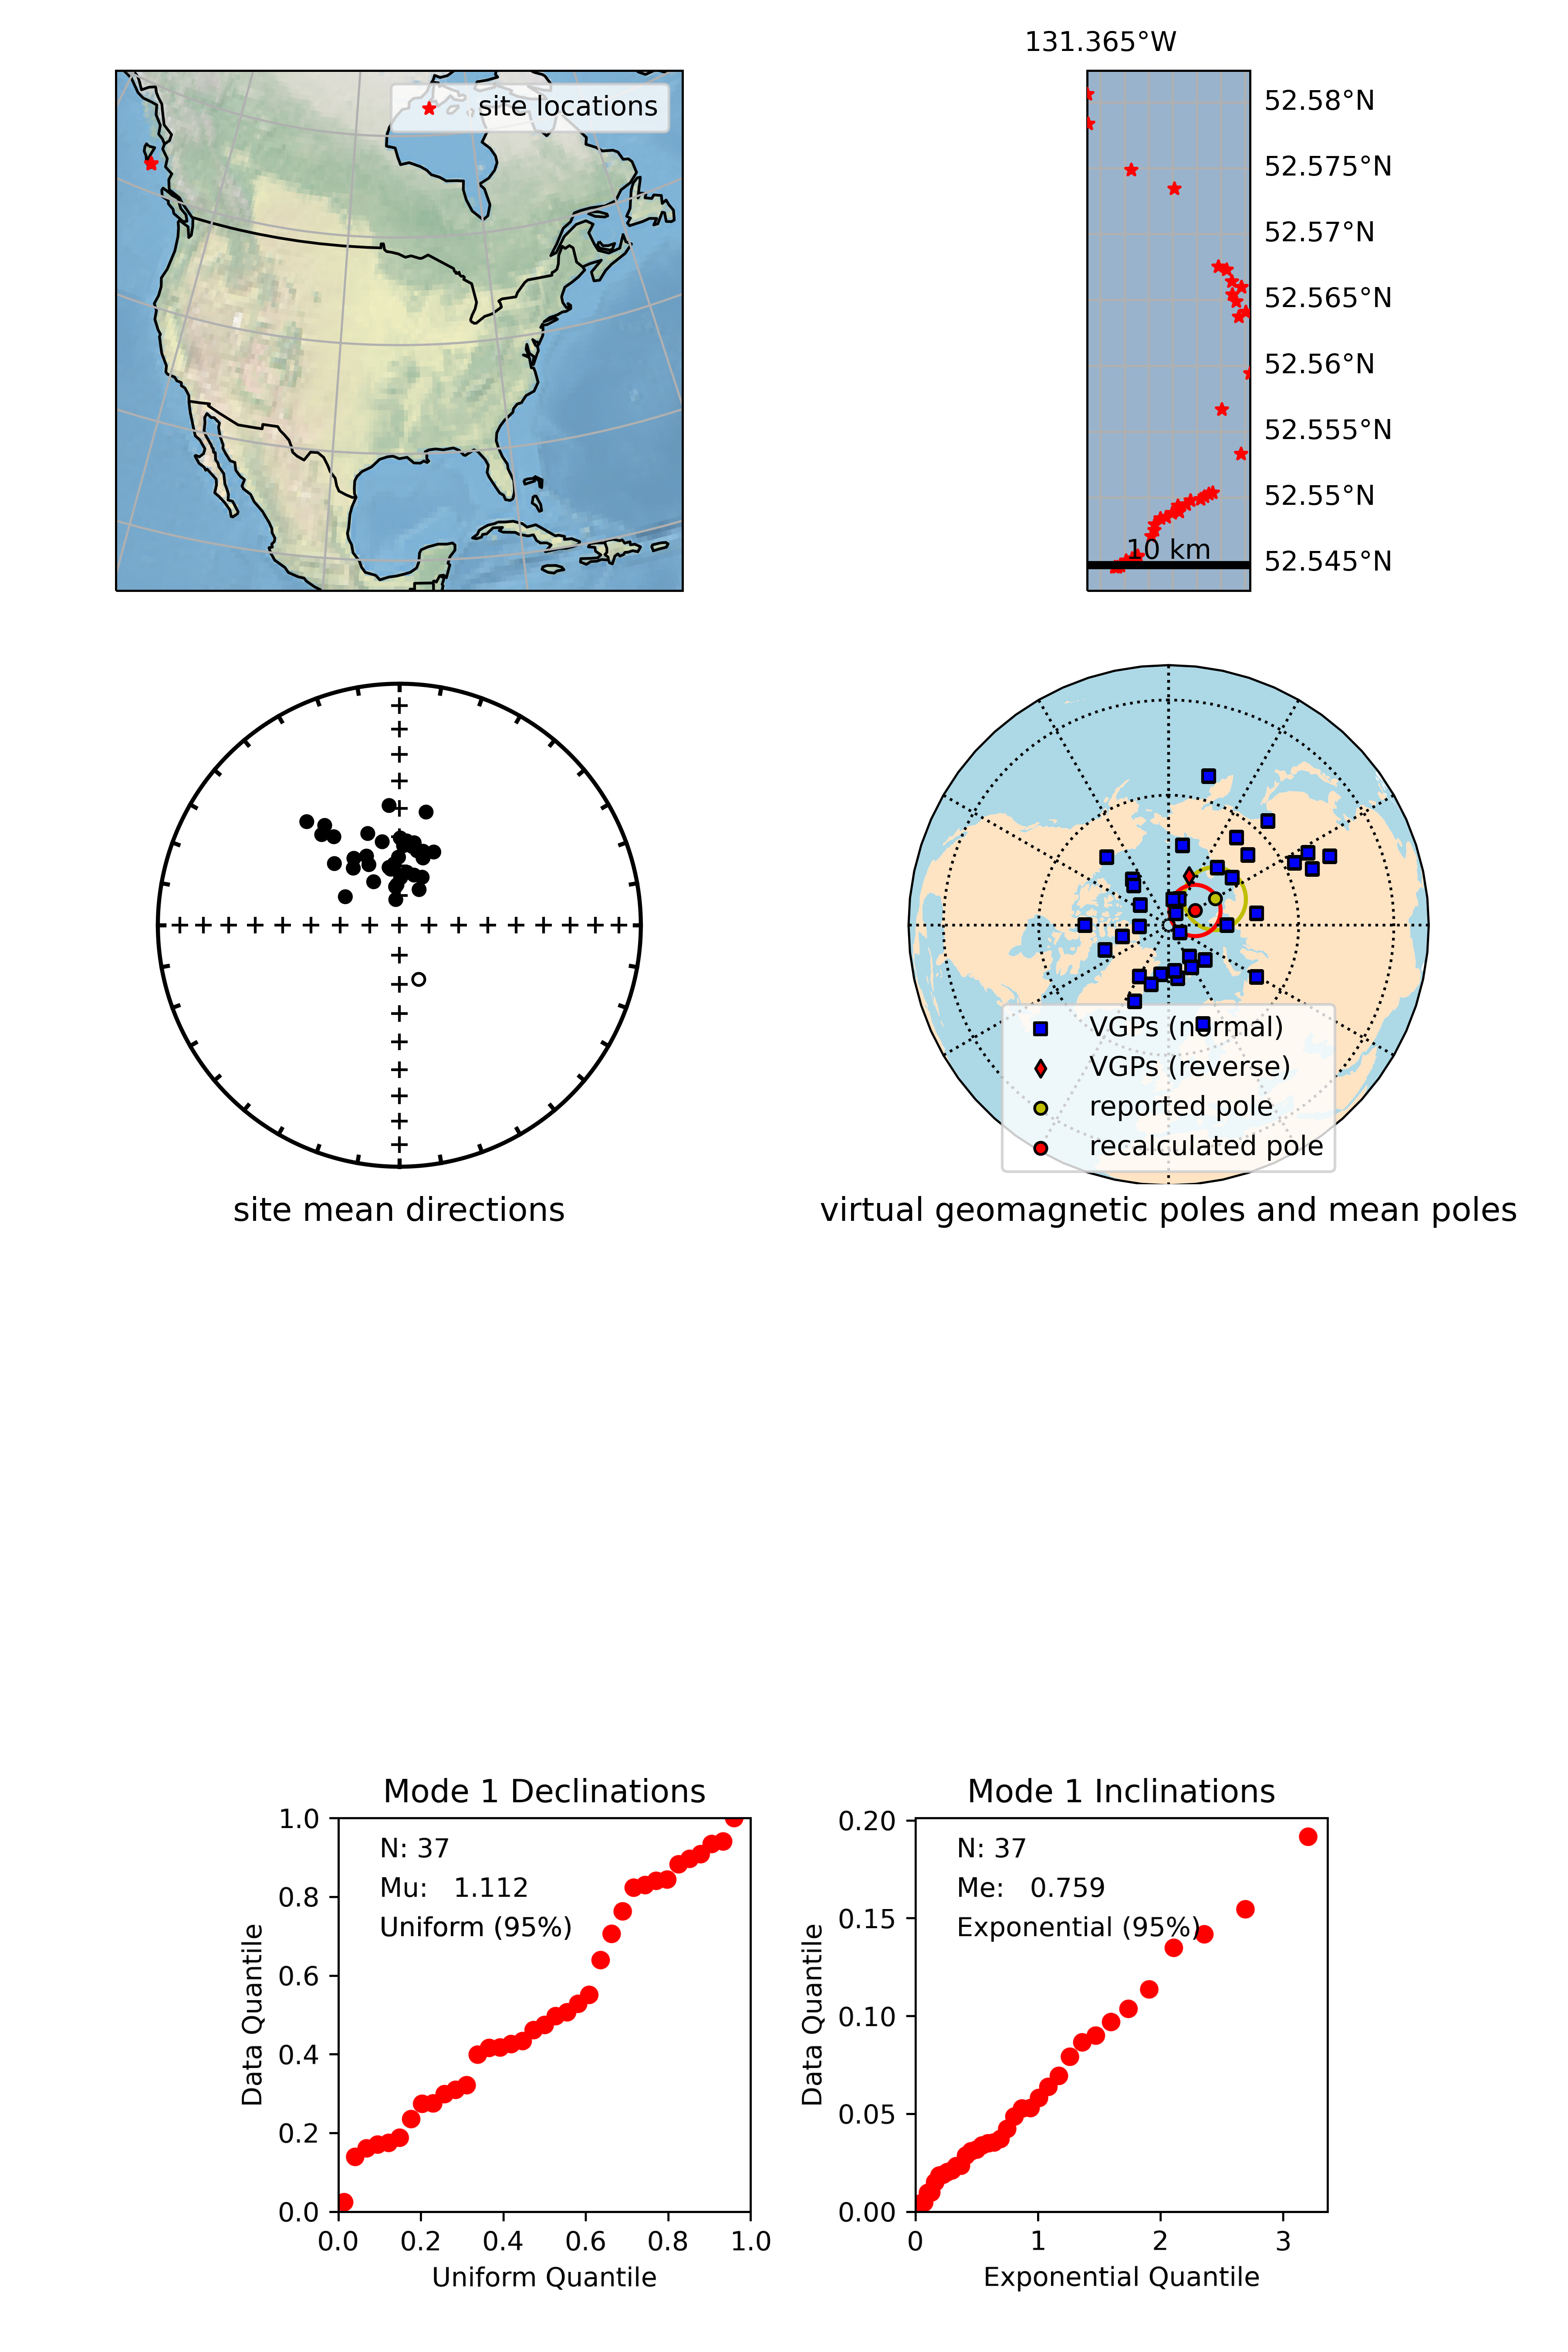
\includegraphics[width=5 in]{./9/1/pole_summary.png}
\caption{Summary of data from locality 9 (Ramsay Island lavas) pole 1 (Irving et al. (2000)).}
\end{figure}

\section{Sierra de Las Cruces}
\subsection{Pole 1}
\begin{tabular}{lllll}
\toprule
{} &   N &  Plat &   Plon &  A95 \\
\midrule
Reported mean pole                                 &  33 &  88.0 &  265.5 &  5.0 \\
Mean pole (calculated from VGPs)                   &  33 &  87.9 &  270.8 &  5.1 \\
Mean pole (calculated from transformed directions) &  33 &  87.9 &  270.6 &  5.1 \\
\bottomrule
\end{tabular}

\begin{tabular}{ll}
\toprule
{} &                                                          result \\
\midrule
Bootstrap reversal test  &                                                            Pass \\
Parametric reversal test &  Pass (angle 3.1º below 11.5º critical angle); C classification \\
Bayesian reversal test   &                                   Common mean: positive support \\
Fisher Q-Q test          &                             Consistent with Fisher distribution \\
\bottomrule
\end{tabular}

\begin{figure}[H]
\centering
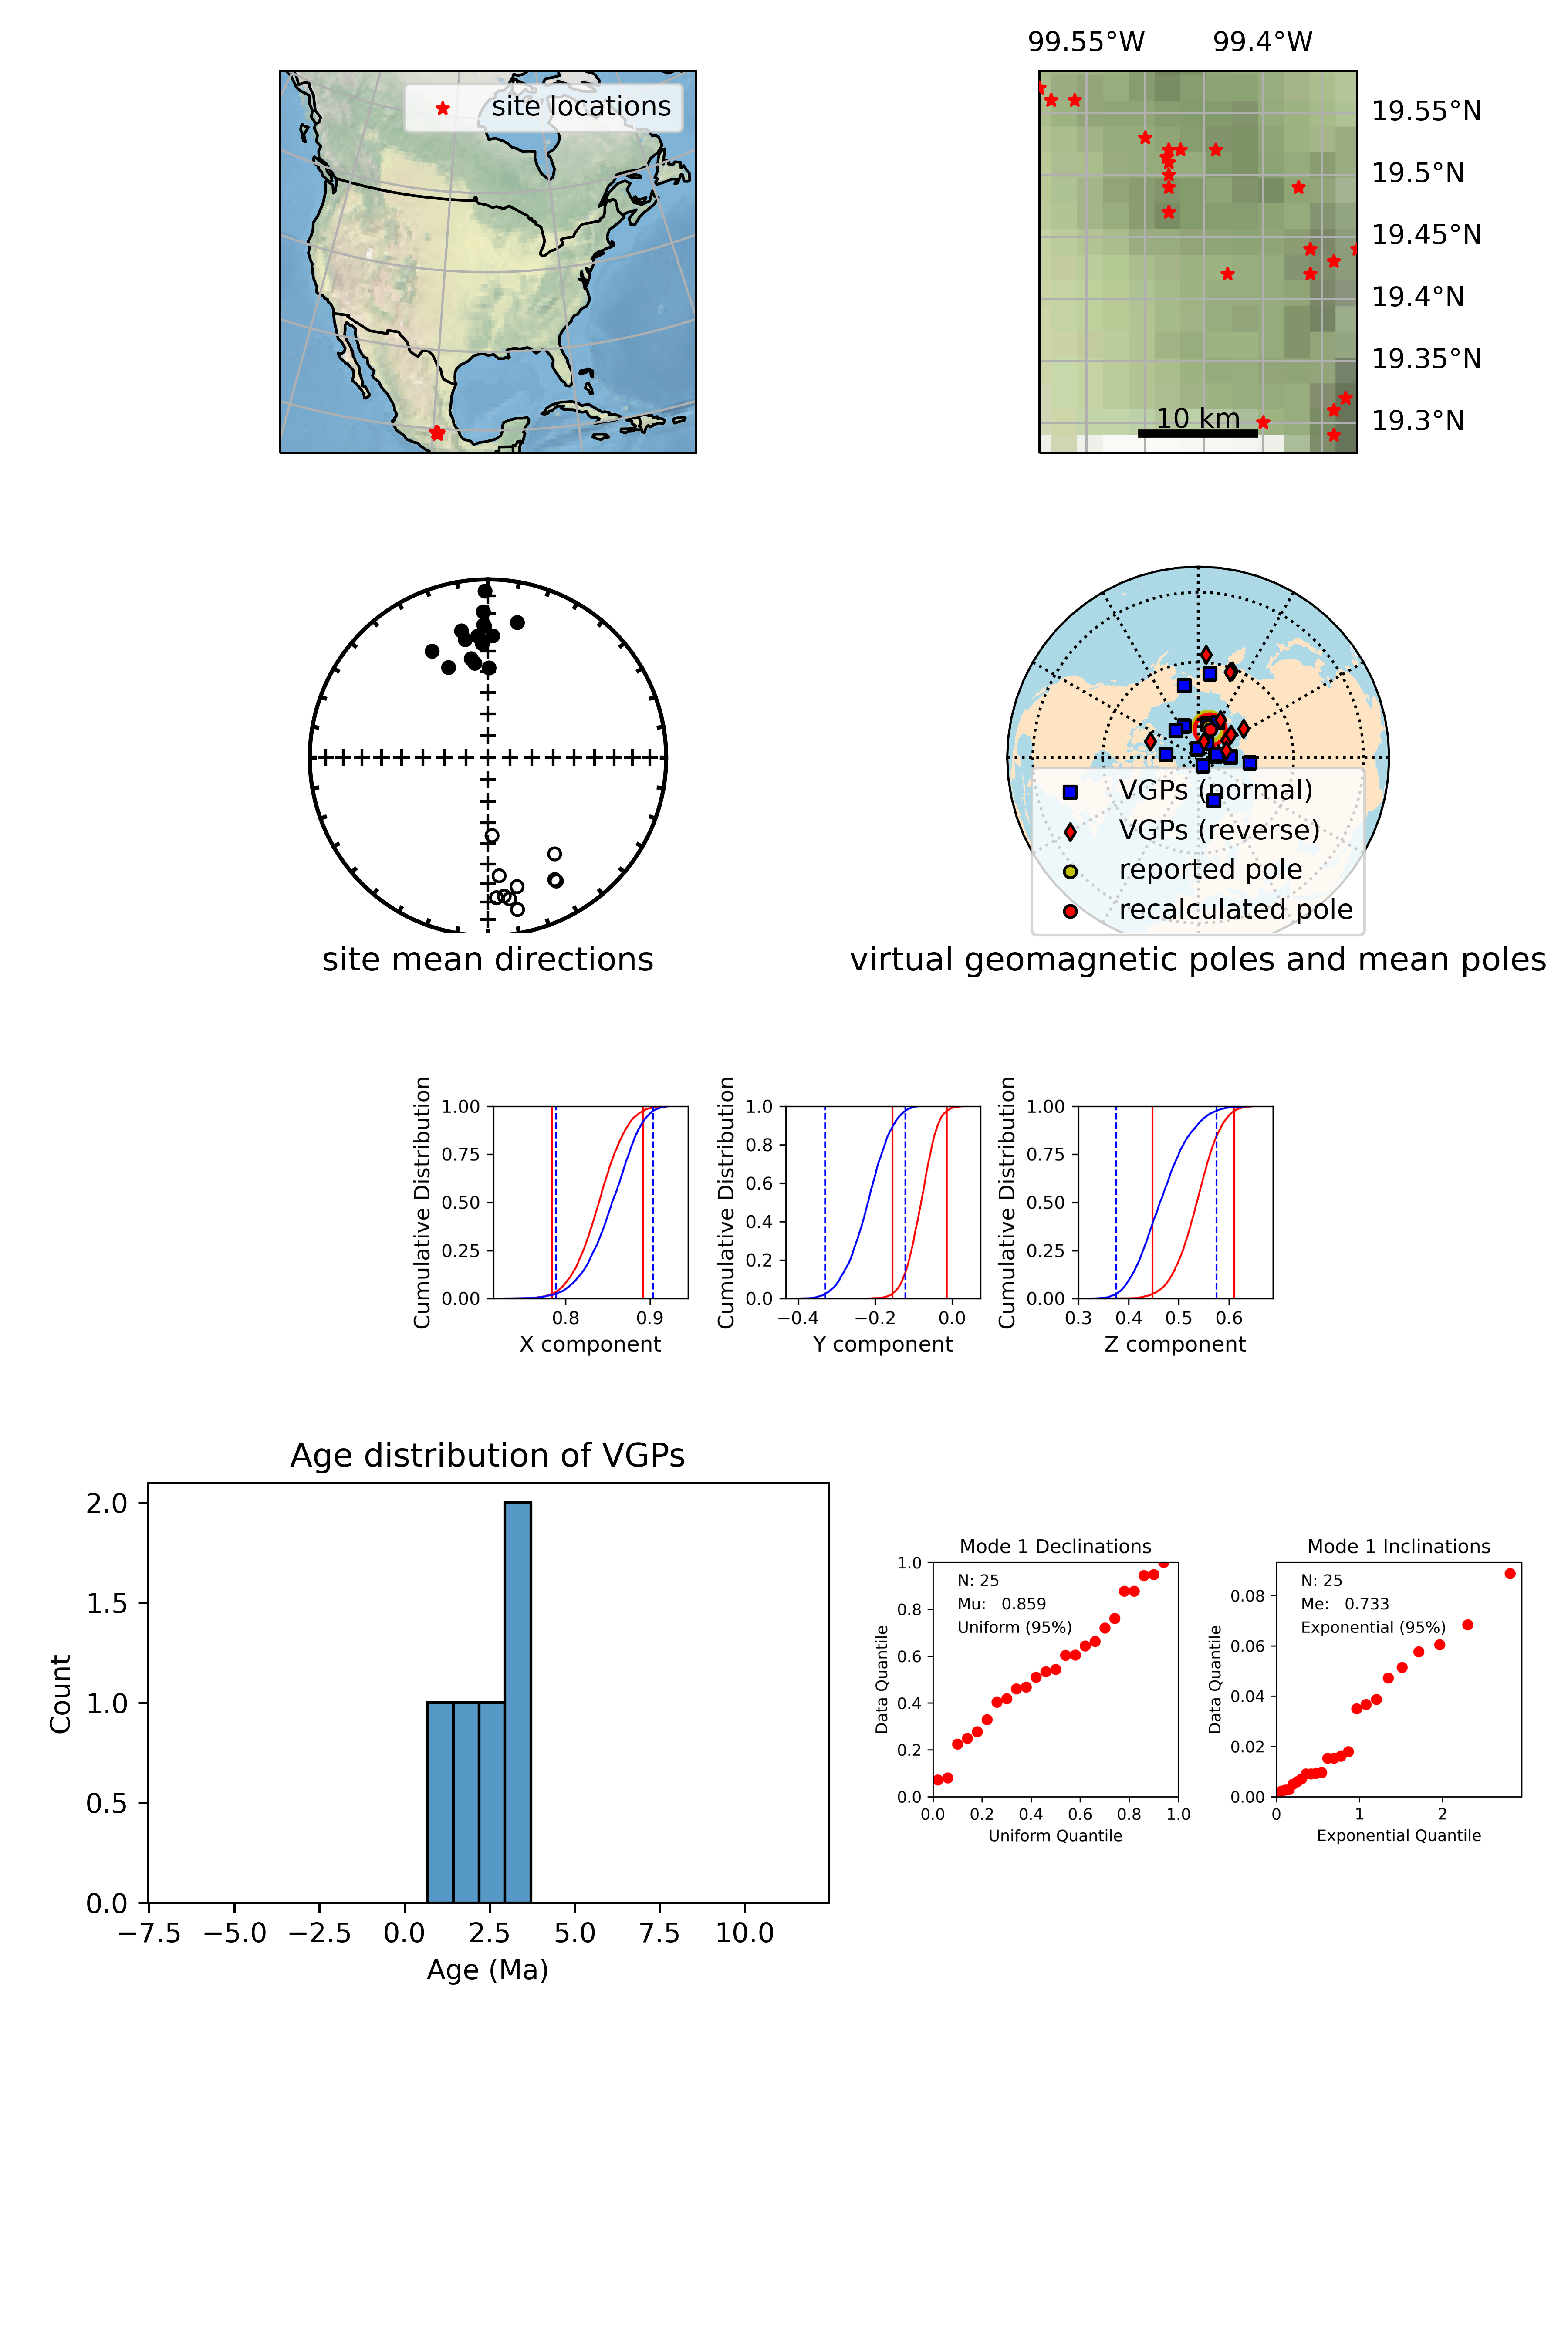
\includegraphics[width=5 in]{./10/1/pole_summary.png}
\caption{Summary of data from locality 10 (Sierra de Las Cruces) pole 1 (Osete et al. (2000)).}
\end{figure}

\section{Snake River Plain}
\subsection{Pole 1}
\begin{tabular}{lllll}
\toprule
{} &   N &  Plat &   Plon &  A95 \\
\midrule
Reported mean pole                                 &  33 &  88.0 &  265.5 &  5.0 \\
Mean pole (calculated from VGPs)                   &  33 &  87.9 &  270.8 &  5.1 \\
Mean pole (calculated from transformed directions) &  33 &  87.9 &  270.6 &  5.1 \\
\bottomrule
\end{tabular}

\begin{tabular}{ll}
\toprule
{} &                                                          result \\
\midrule
Bootstrap reversal test  &                                                            Pass \\
Parametric reversal test &  Pass (angle 3.1º below 11.5º critical angle); C classification \\
Bayesian reversal test   &                                   Common mean: positive support \\
Fisher Q-Q test          &                             Consistent with Fisher distribution \\
\bottomrule
\end{tabular}

\begin{figure}[H]
\centering
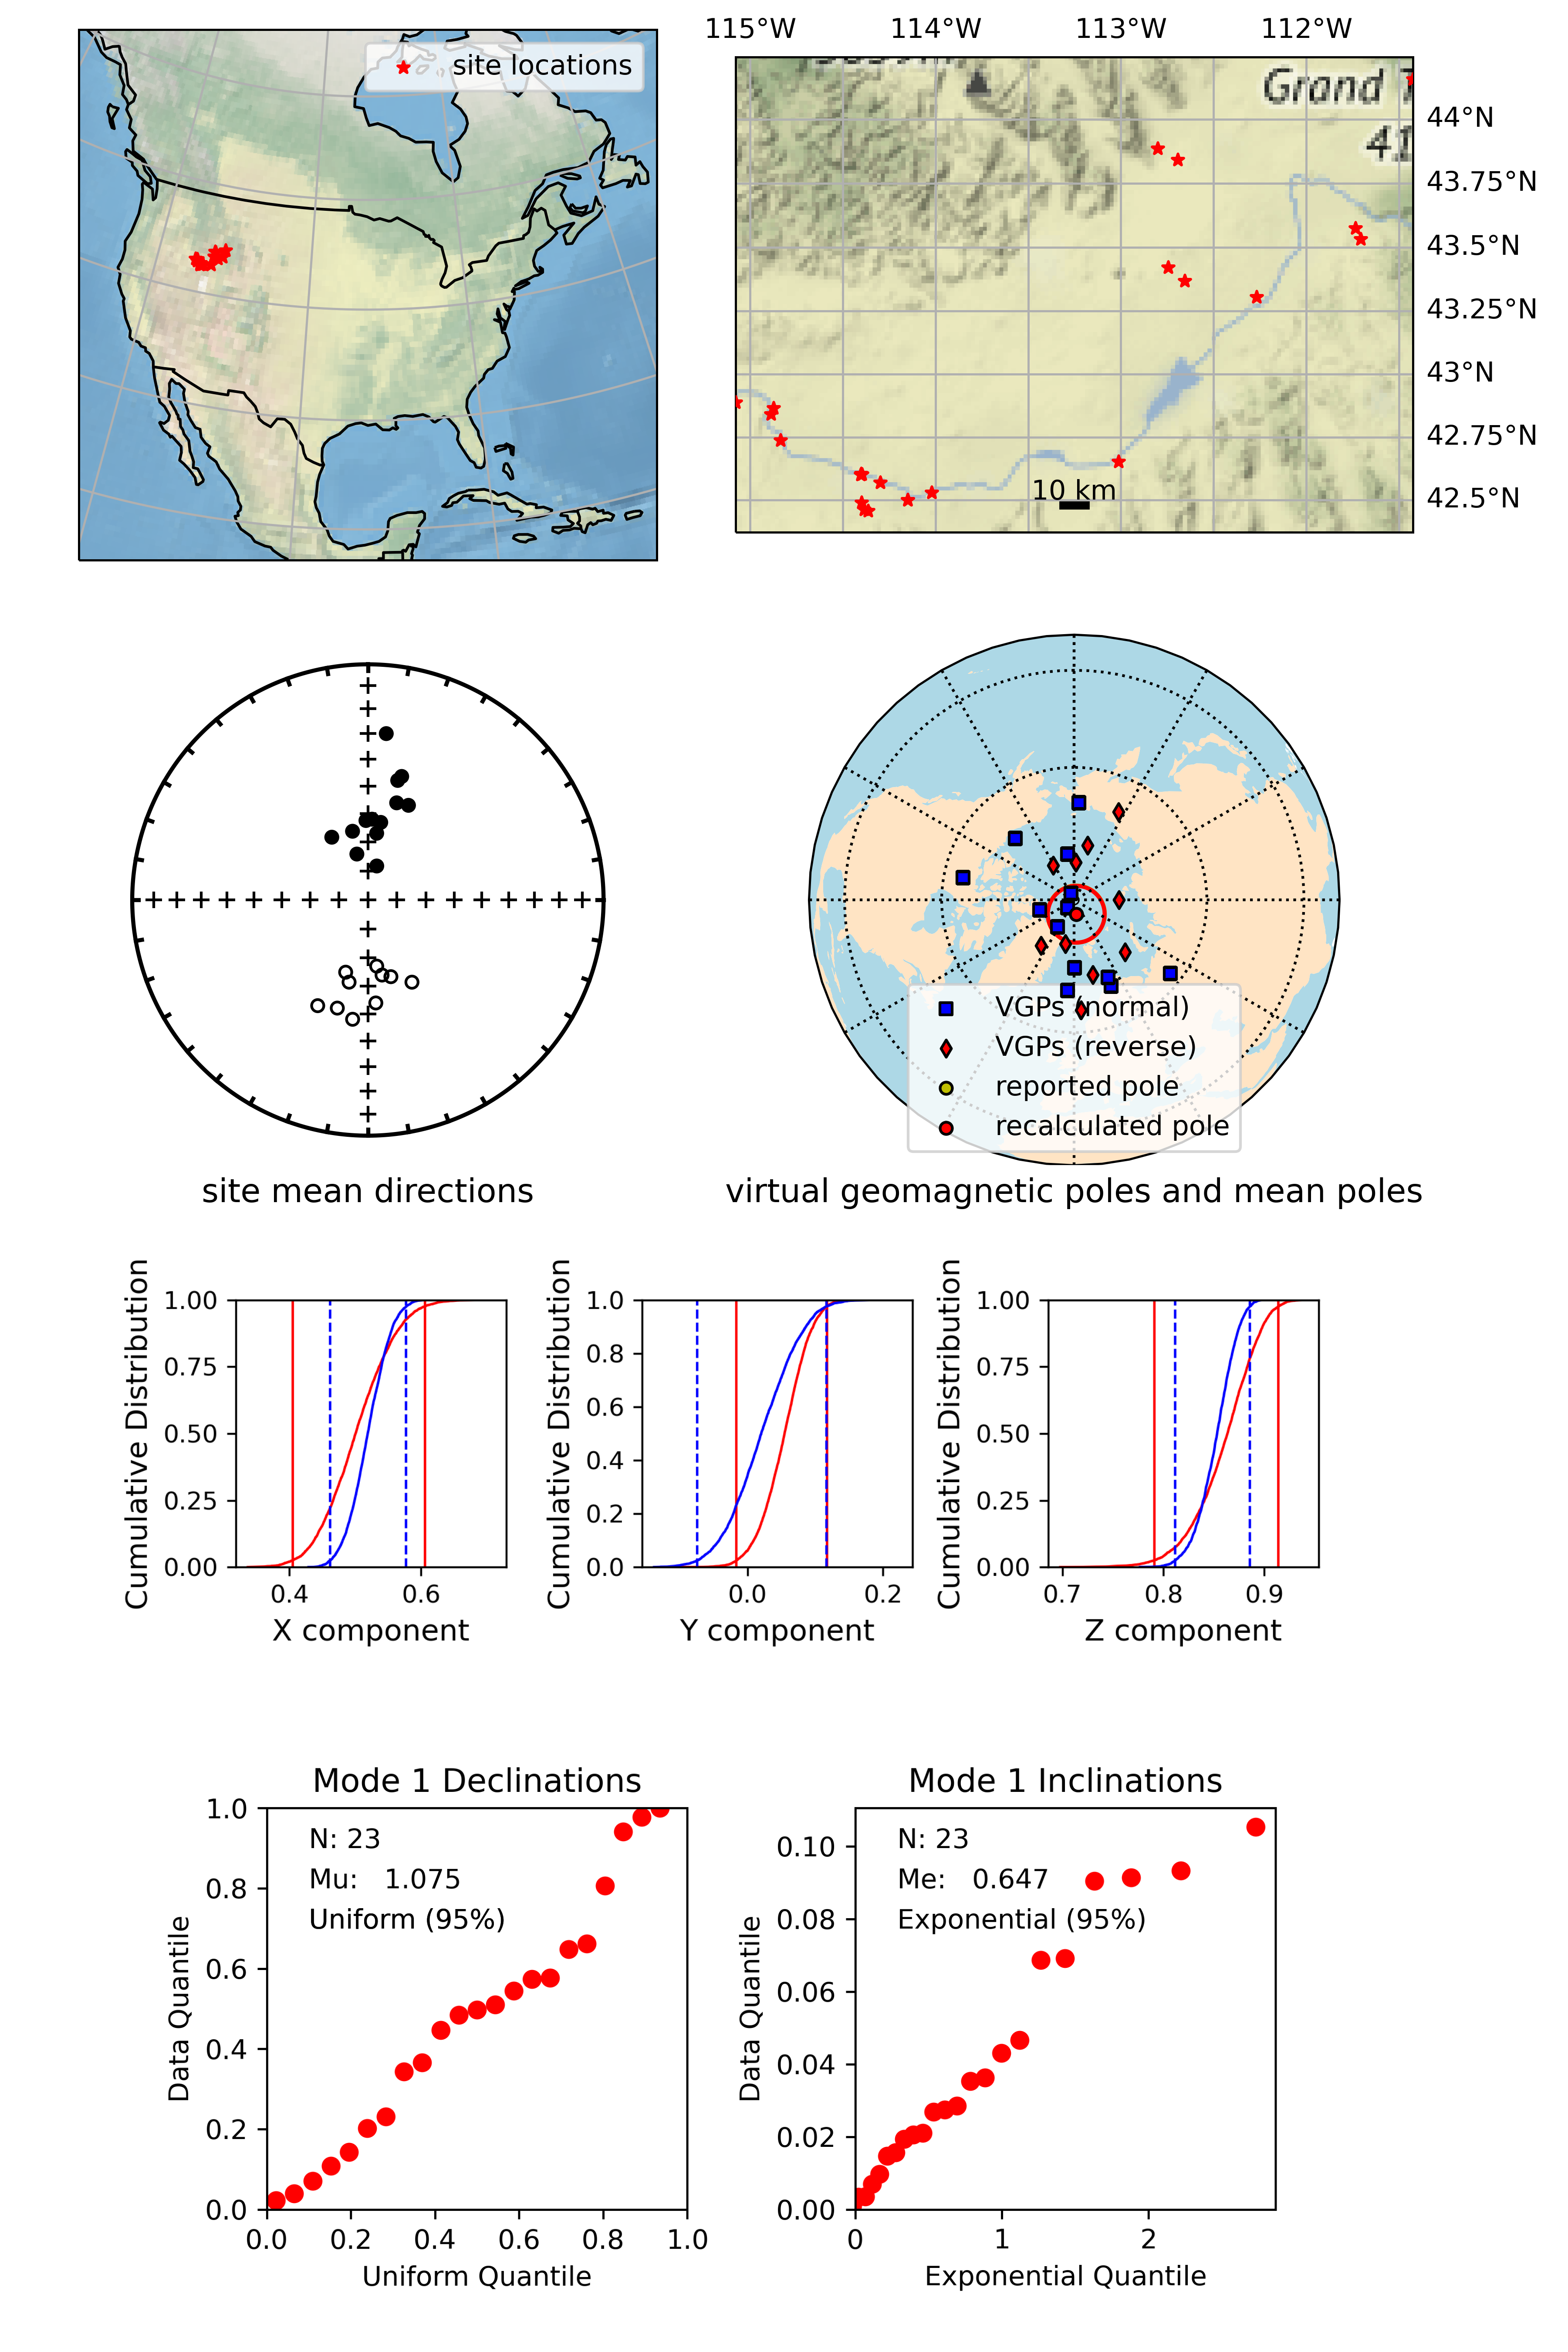
\includegraphics[width=5 in]{./11/1/pole_summary.png}
\caption{Summary of data from locality 11 (Snake River Plain) pole 1 (Tauxe et al. (2004)).}
\end{figure}

\section{Sonoma volcanics}
\subsection{Pole 1}
\begin{tabular}{lllll}
\toprule
{} &   N &  Plat &   Plon &  A95 \\
\midrule
Reported mean pole                                 &  33 &  88.0 &  265.5 &  5.0 \\
Mean pole (calculated from VGPs)                   &  33 &  87.9 &  270.8 &  5.1 \\
Mean pole (calculated from transformed directions) &  33 &  87.9 &  270.6 &  5.1 \\
\bottomrule
\end{tabular}

\begin{tabular}{ll}
\toprule
{} &                                                          result \\
\midrule
Bootstrap reversal test  &                                                            Pass \\
Parametric reversal test &  Pass (angle 3.1º below 11.5º critical angle); C classification \\
Bayesian reversal test   &                                   Common mean: positive support \\
Fisher Q-Q test          &                             Consistent with Fisher distribution \\
\bottomrule
\end{tabular}

\begin{figure}[H]
\centering
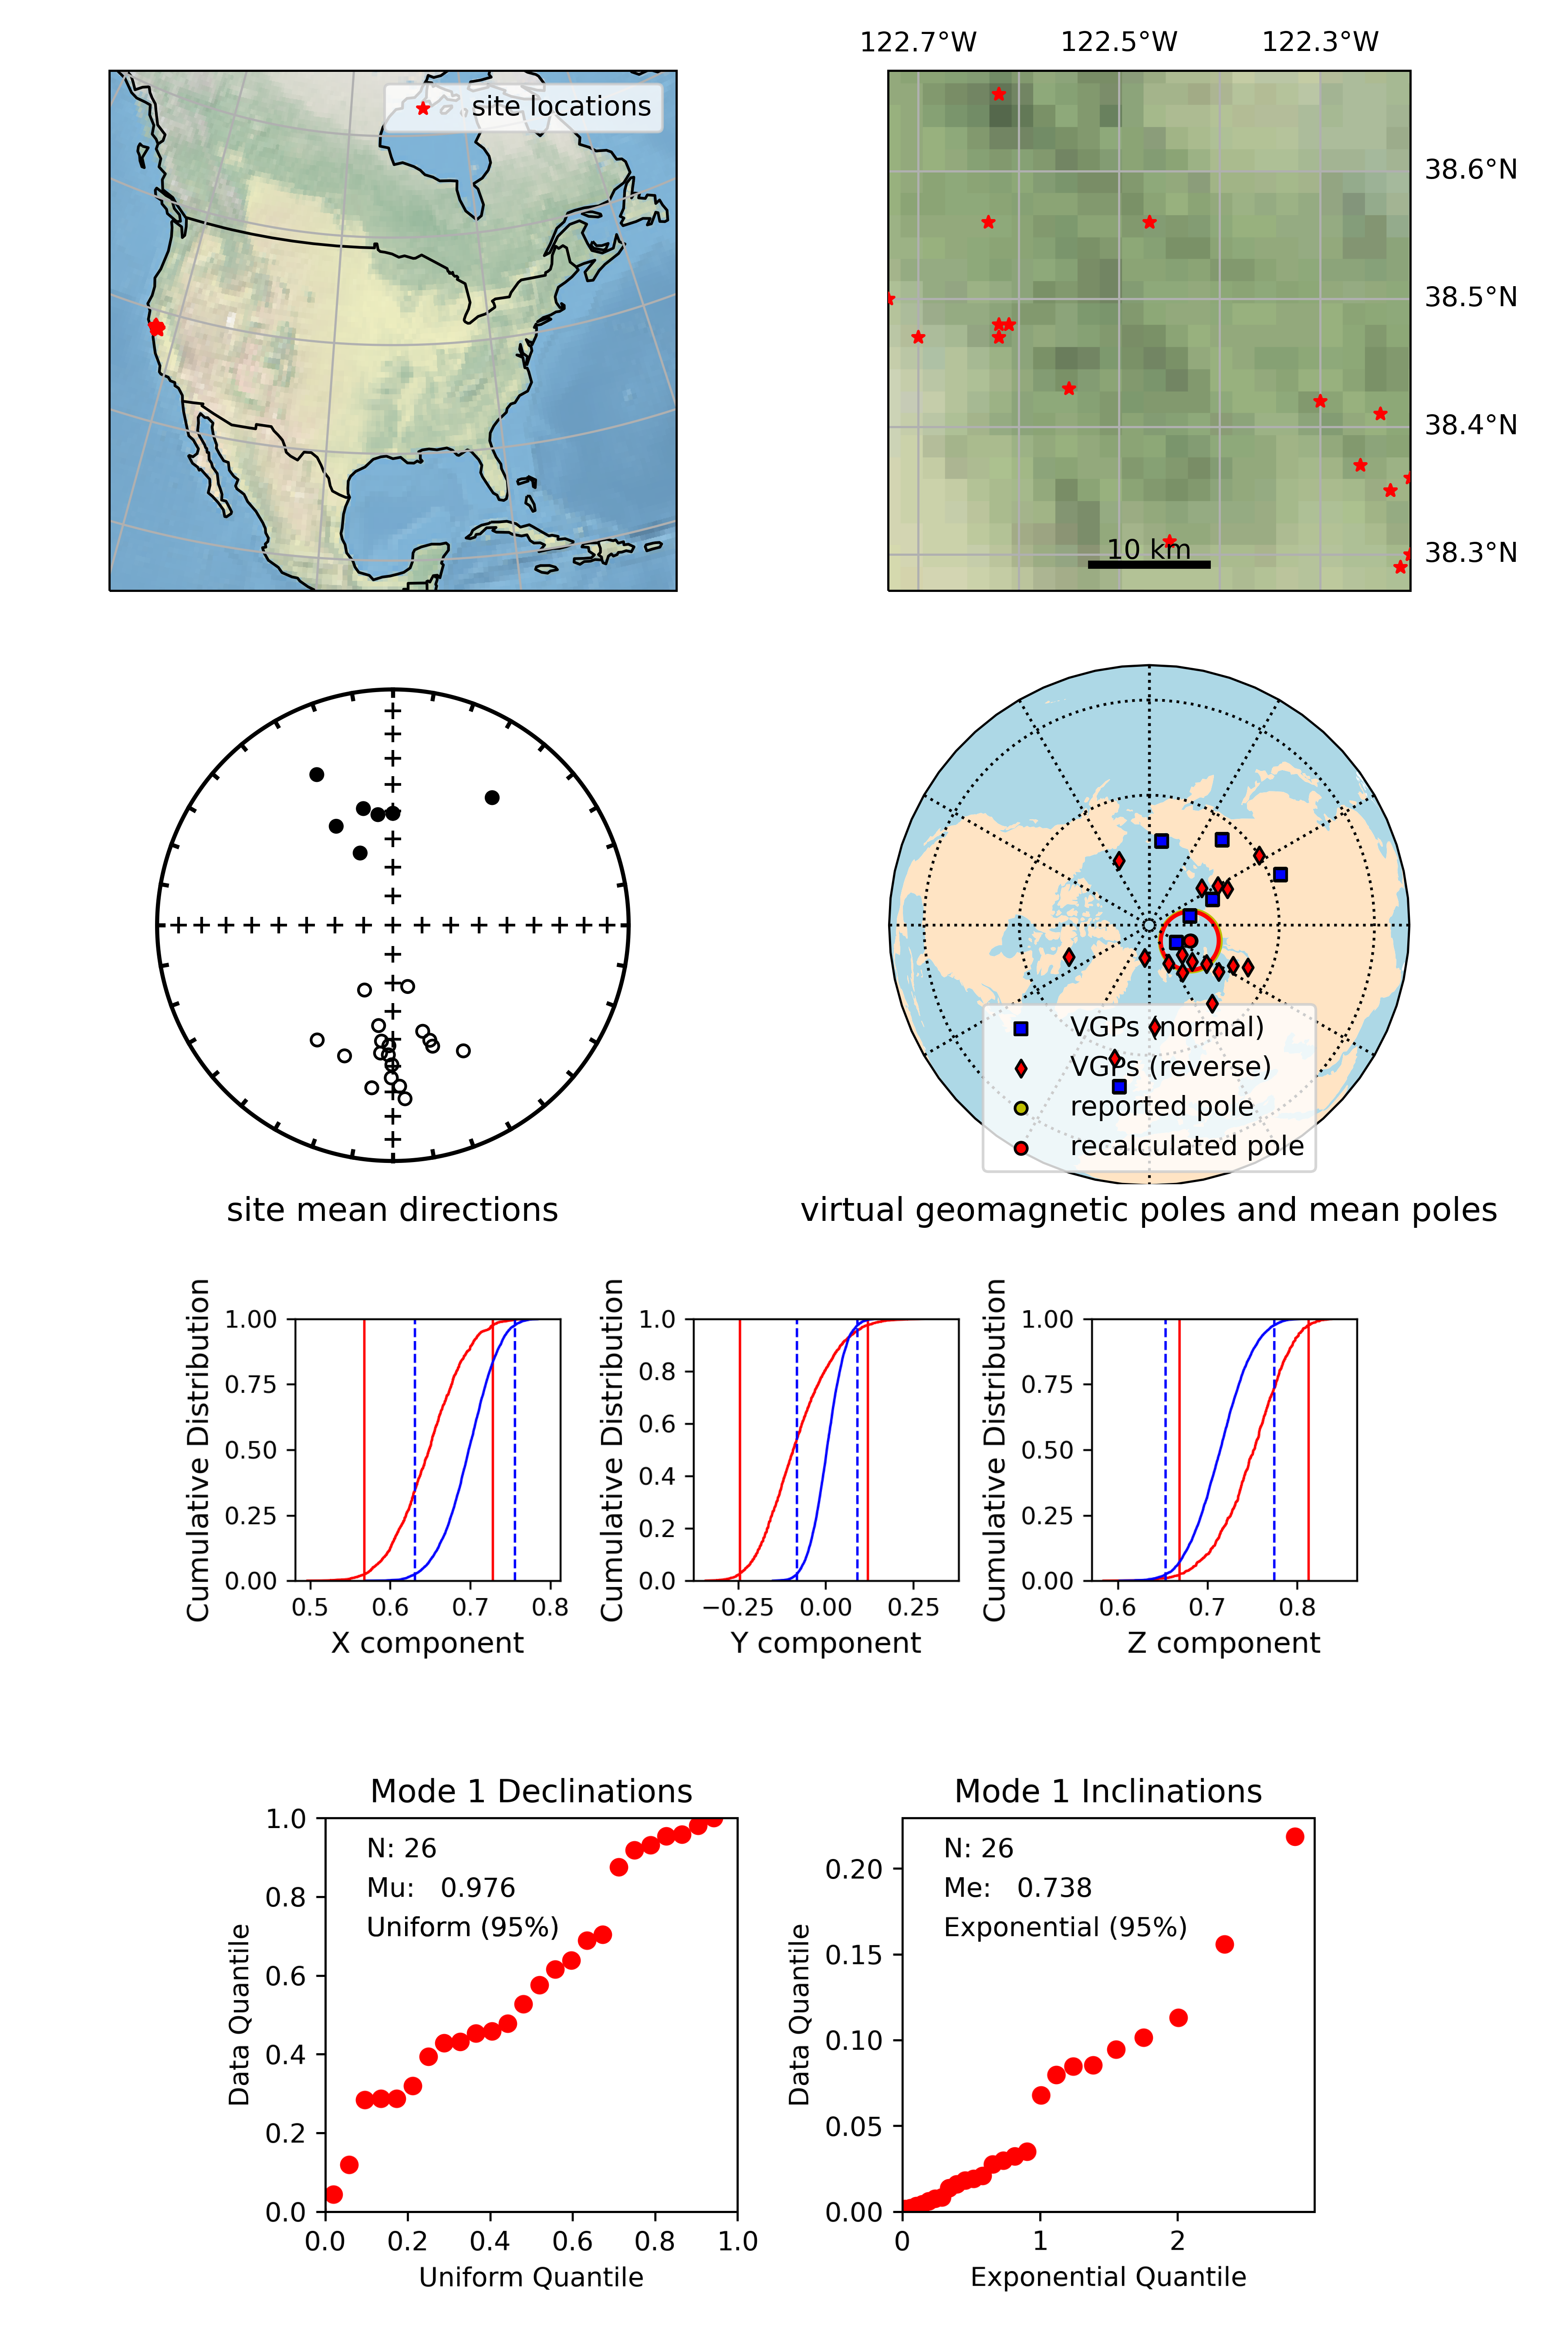
\includegraphics[width=5 in]{./12/1/pole_summary.png}
\caption{Summary of data from locality 12 (Sonoma volcanics) pole 1 (Mankinen (1989); Mankinen (1972)).}
\end{figure}

\section{Mistastin Lake impact}
\subsection{Pole 1}
\begin{tabular}{lllll}
\toprule
{} &   N &  Plat &   Plon &  A95 \\
\midrule
Reported mean pole                                 &  33 &  88.0 &  265.5 &  5.0 \\
Mean pole (calculated from VGPs)                   &  33 &  87.9 &  270.8 &  5.1 \\
Mean pole (calculated from transformed directions) &  33 &  87.9 &  270.6 &  5.1 \\
\bottomrule
\end{tabular}

\begin{tabular}{ll}
\toprule
{} &                                                          result \\
\midrule
Bootstrap reversal test  &                                                            Pass \\
Parametric reversal test &  Pass (angle 3.1º below 11.5º critical angle); C classification \\
Bayesian reversal test   &                                   Common mean: positive support \\
Fisher Q-Q test          &                             Consistent with Fisher distribution \\
\bottomrule
\end{tabular}

\begin{figure}[H]
\centering
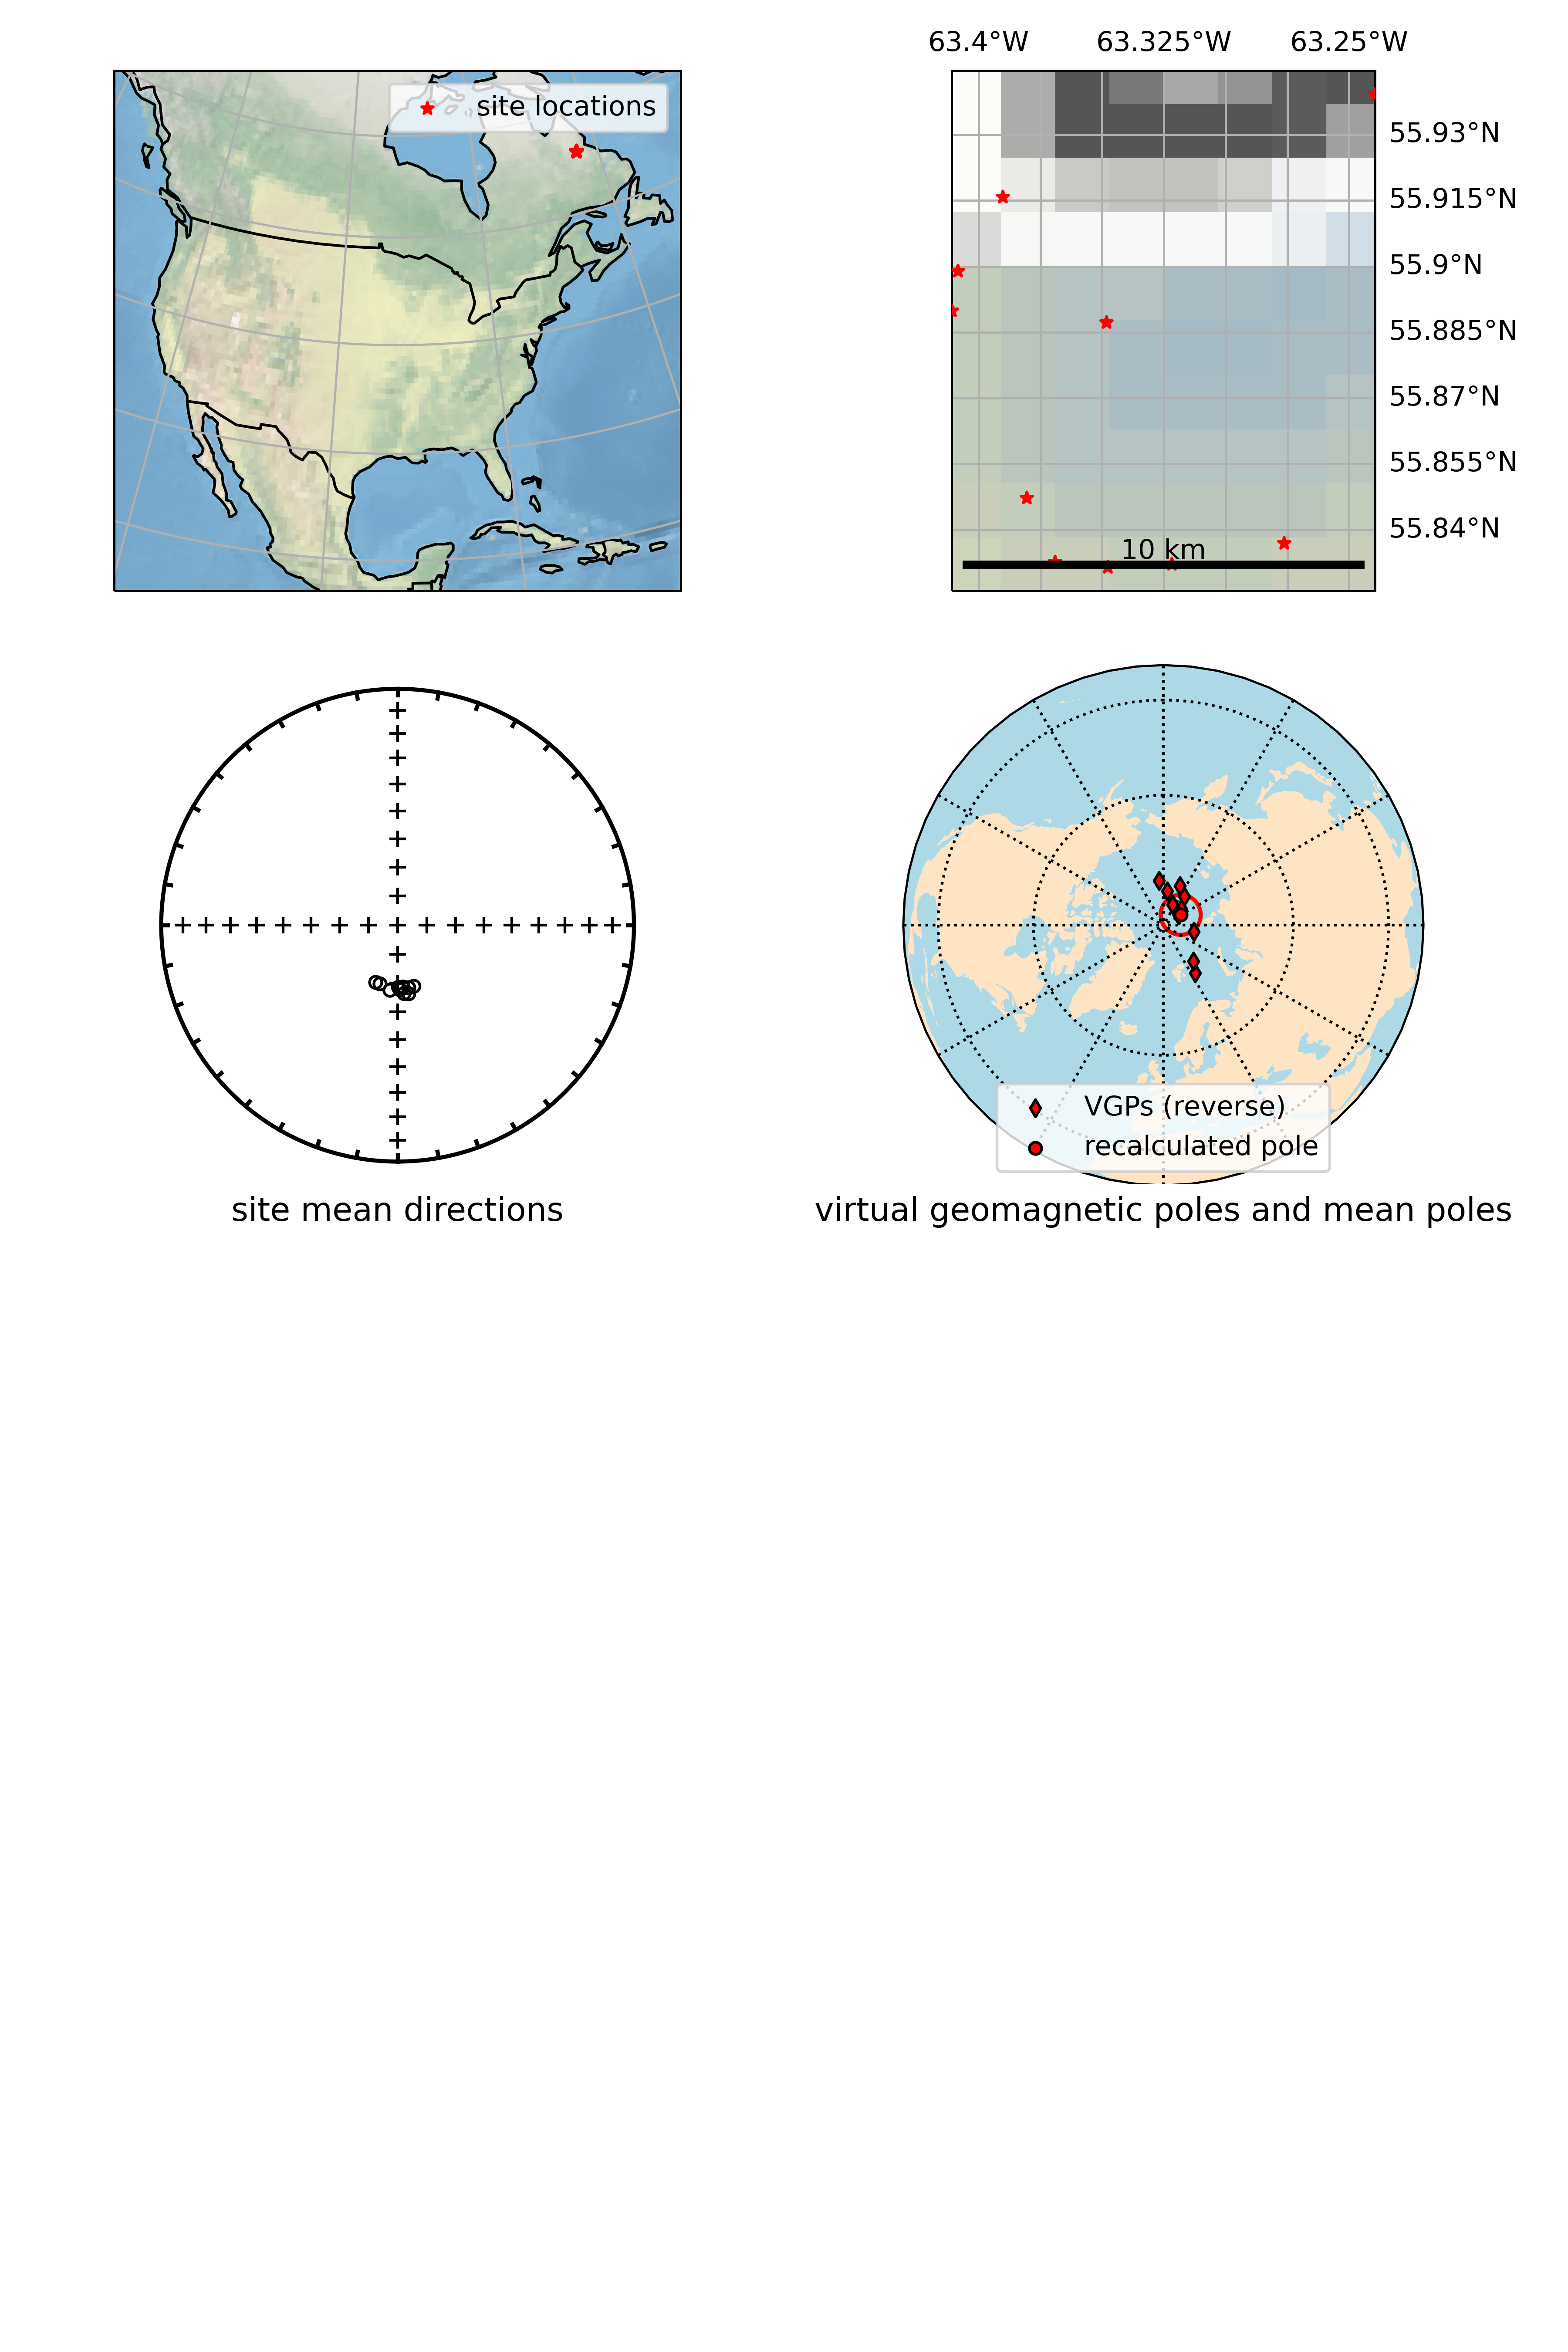
\includegraphics[width=5 in]{./13/1/pole_summary.png}
\caption{Summary of data from locality 13 (Mistastin Lake impact) pole 1 (Currie and Larochelle (1969)).}
\end{figure}

\subsection{Pole 2}
\begin{tabular}{lllll}
\toprule
{} &   N &  Plat &   Plon &  A95 \\
\midrule
Reported mean pole                                 &  33 &  88.0 &  265.5 &  5.0 \\
Mean pole (calculated from VGPs)                   &  33 &  87.9 &  270.8 &  5.1 \\
Mean pole (calculated from transformed directions) &  33 &  87.9 &  270.6 &  5.1 \\
\bottomrule
\end{tabular}

\begin{tabular}{ll}
\toprule
{} &                                                          result \\
\midrule
Bootstrap reversal test  &                                                            Pass \\
Parametric reversal test &  Pass (angle 3.1º below 11.5º critical angle); C classification \\
Bayesian reversal test   &                                   Common mean: positive support \\
Fisher Q-Q test          &                             Consistent with Fisher distribution \\
\bottomrule
\end{tabular}

\begin{figure}[H]
\centering
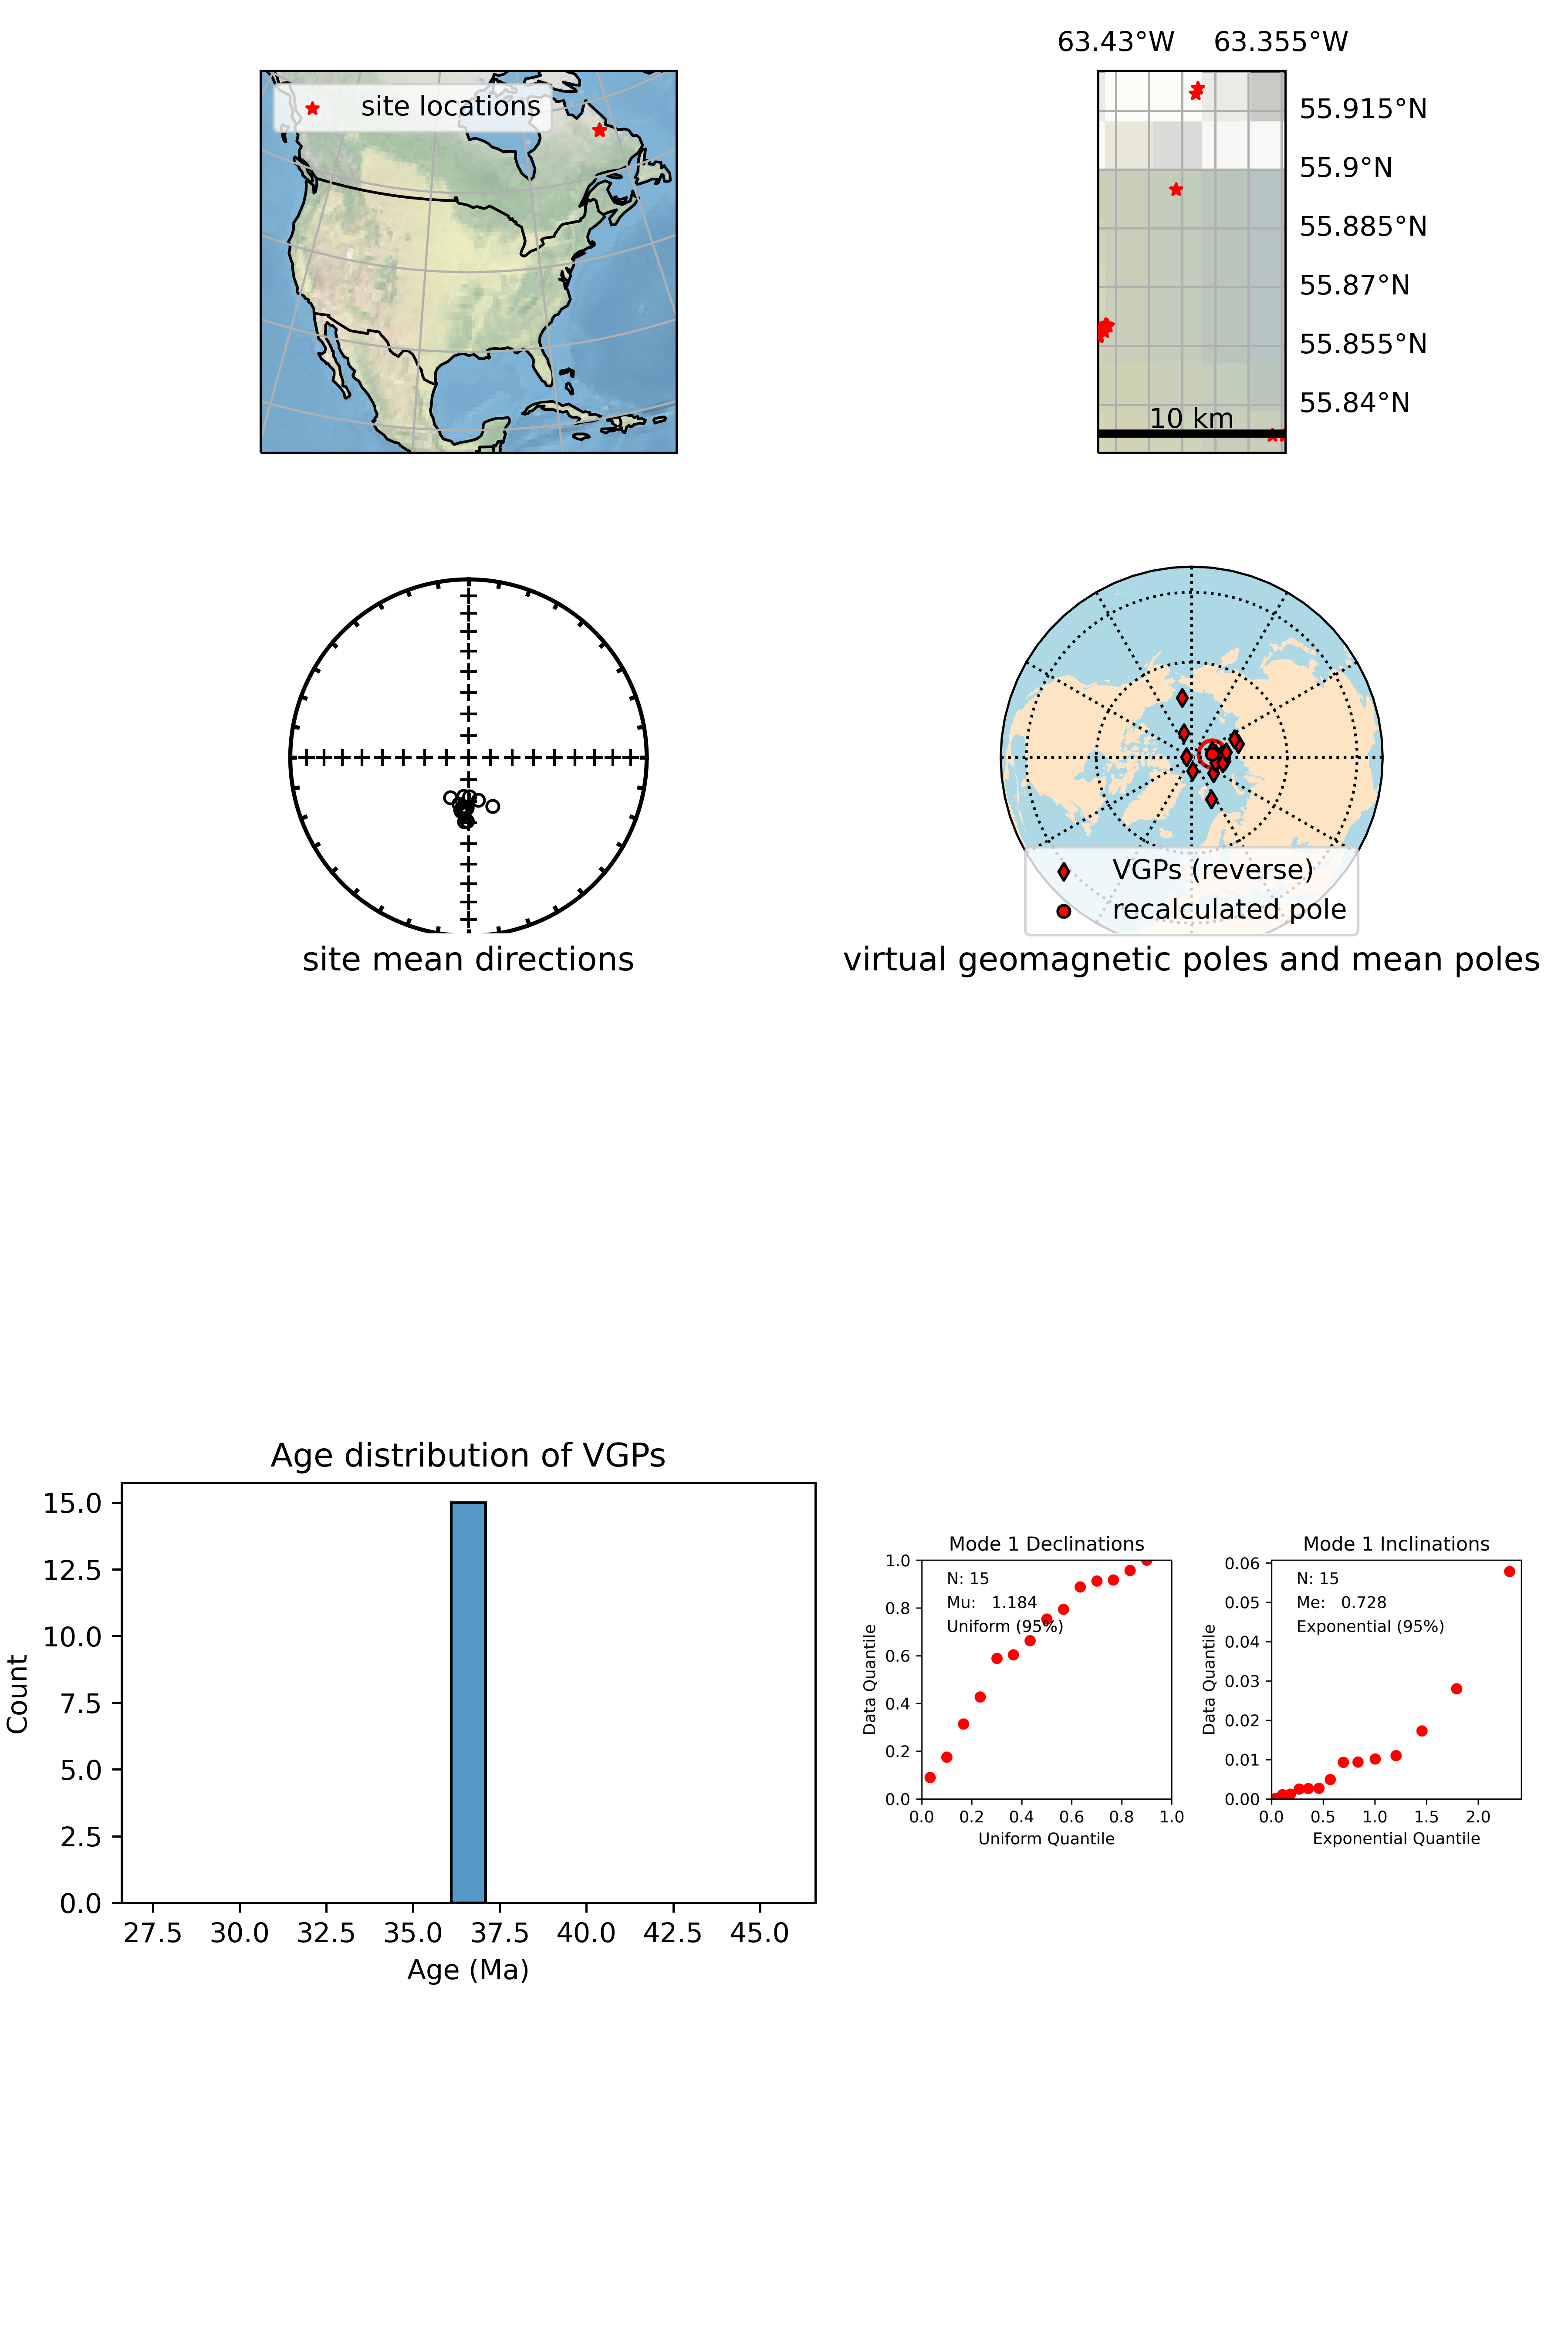
\includegraphics[width=5 in]{./13/2/pole_summary.png}
\caption{Summary of data from locality 13 (Mistastin Lake impact) pole 2 (Herve et al. (2015)).}
\end{figure}

\section{Bighorn Basin sediments}
\subsection{Pole 1}
\begin{tabular}{lllll}
\toprule
{} &   N &  Plat &   Plon &  A95 \\
\midrule
Reported mean pole                                 &  33 &  88.0 &  265.5 &  5.0 \\
Mean pole (calculated from VGPs)                   &  33 &  87.9 &  270.8 &  5.1 \\
Mean pole (calculated from transformed directions) &  33 &  87.9 &  270.6 &  5.1 \\
\bottomrule
\end{tabular}

\begin{tabular}{ll}
\toprule
{} &                                                          result \\
\midrule
Bootstrap reversal test  &                                                            Pass \\
Parametric reversal test &  Pass (angle 3.1º below 11.5º critical angle); C classification \\
Bayesian reversal test   &                                   Common mean: positive support \\
Fisher Q-Q test          &                             Consistent with Fisher distribution \\
\bottomrule
\end{tabular}

\begin{figure}[H]
\centering
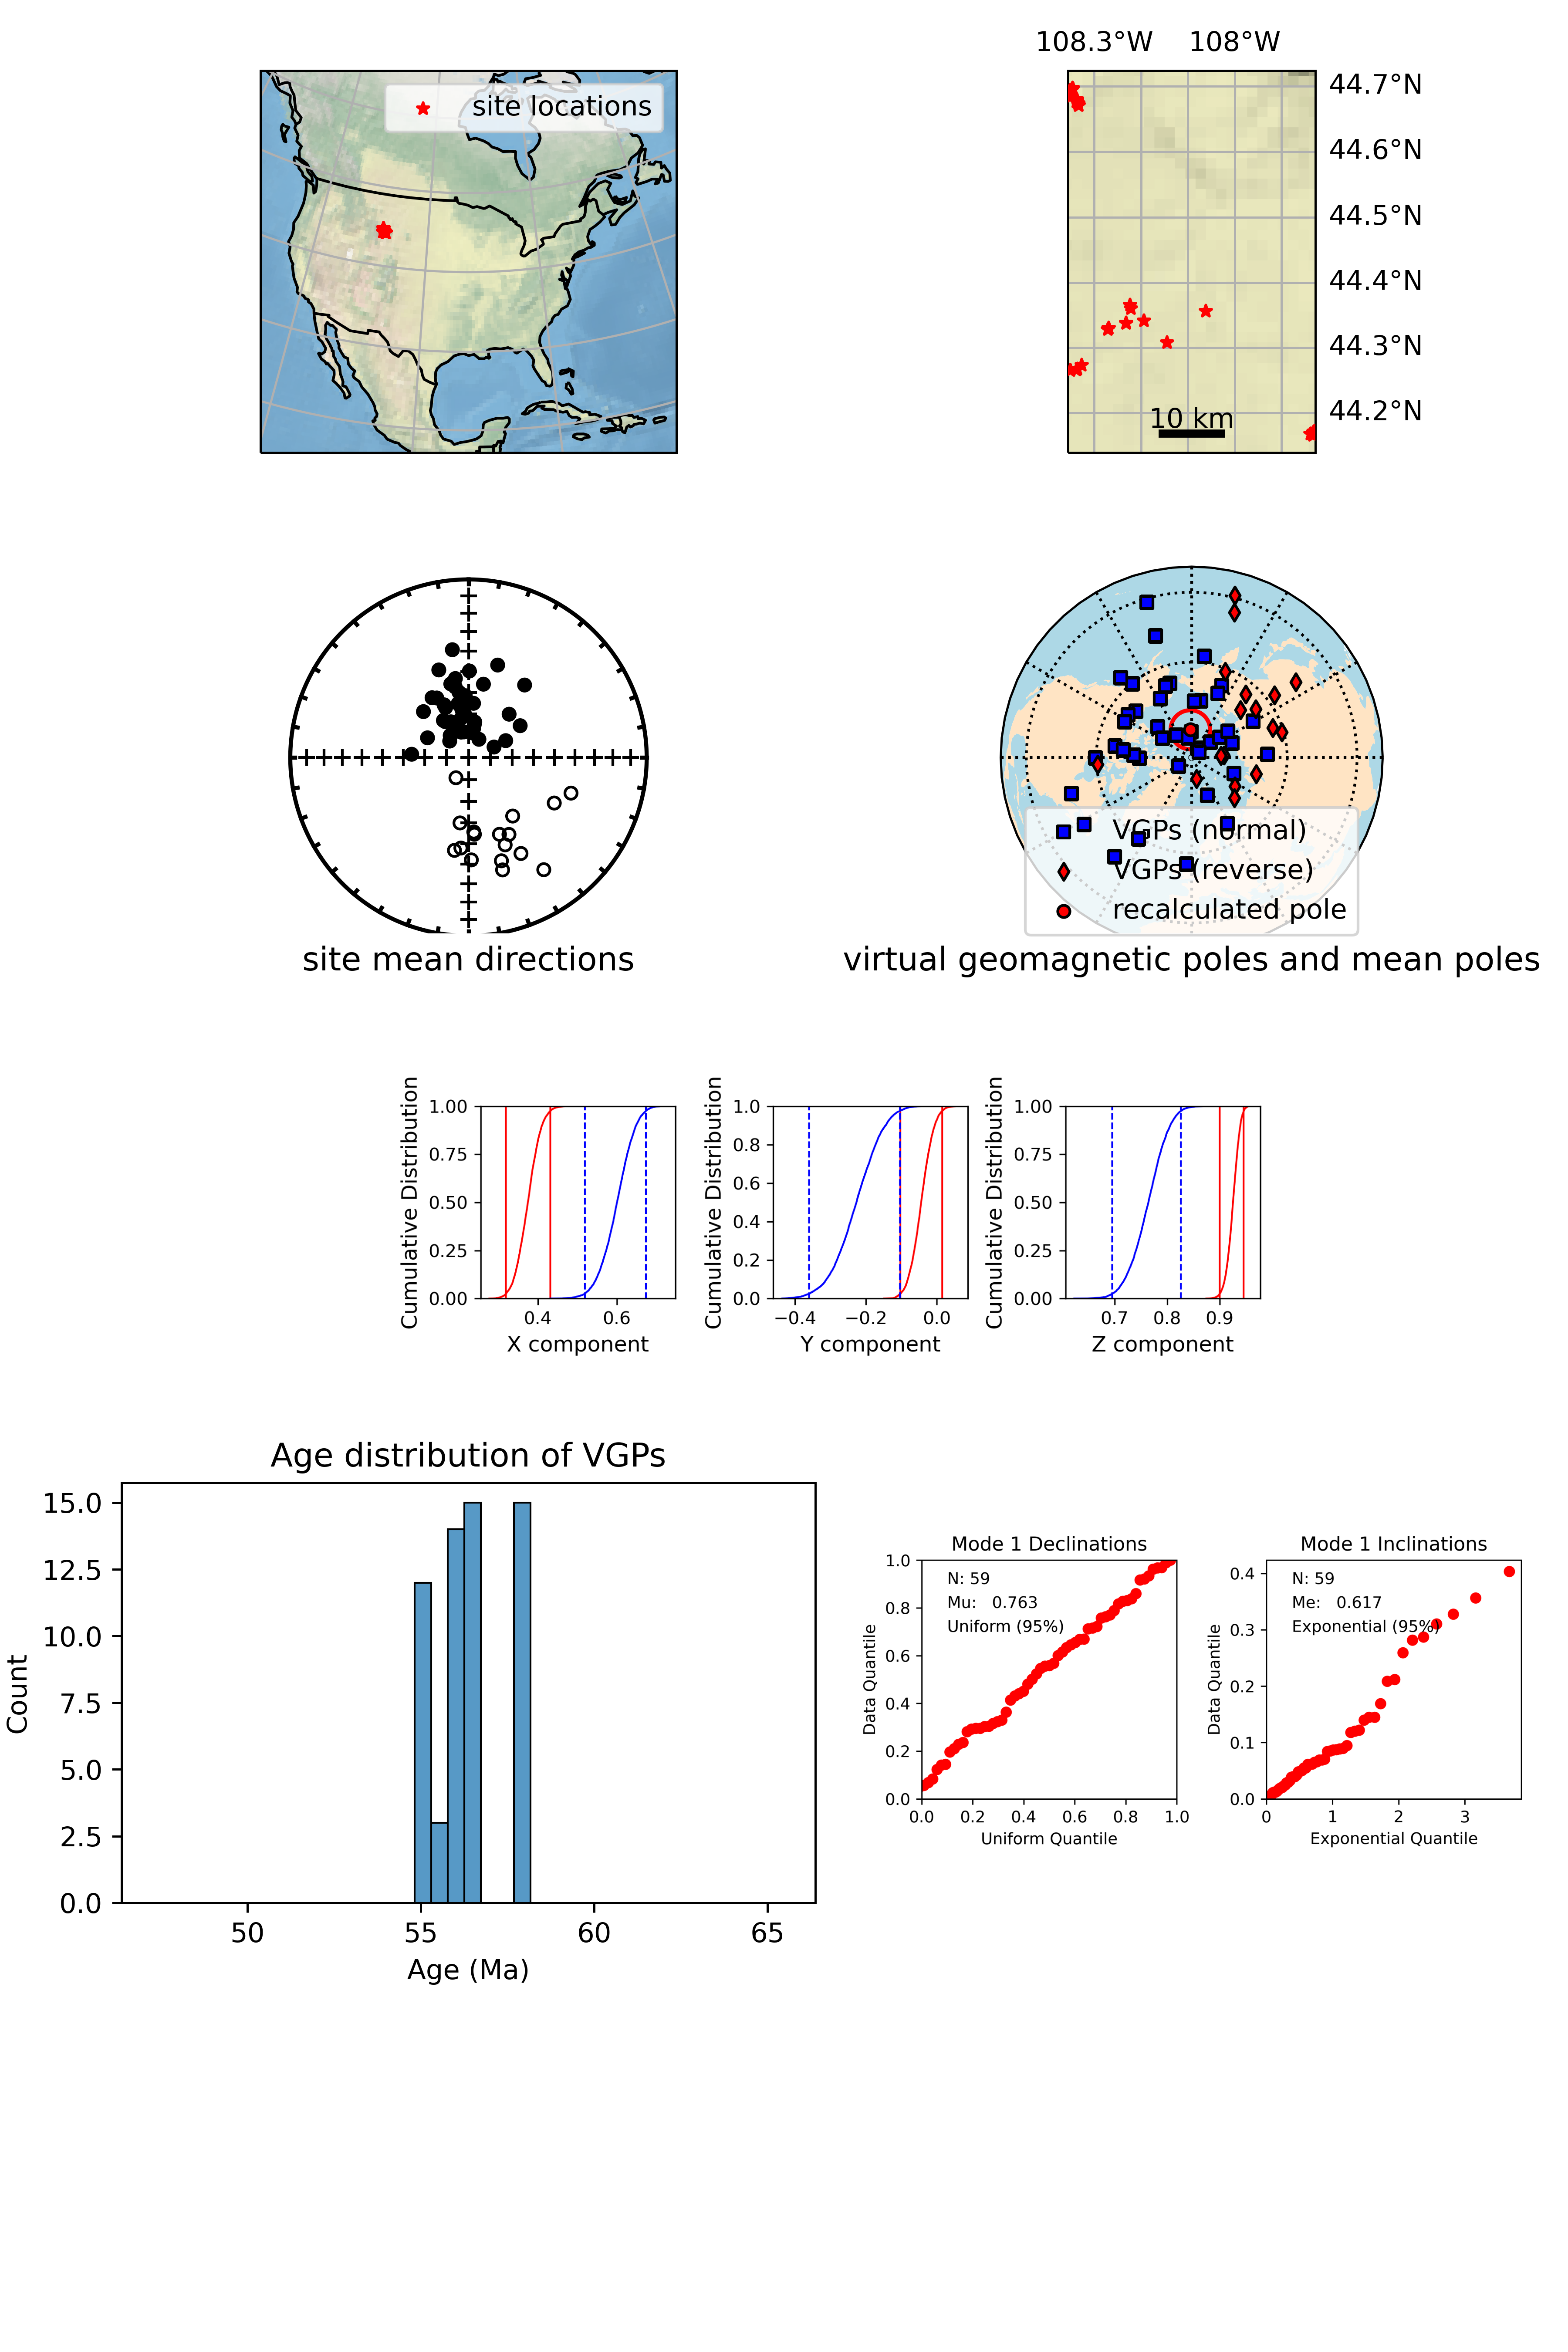
\includegraphics[width=5 in]{./14/1/pole_summary.png}
\caption{Summary of data from locality 14 (Bighorn Basin sediments) pole 1 (Clyde et al. (2007)).}
\end{figure}

\section{Absaroka volcanics}
\subsection{Pole 1}
\begin{tabular}{lllll}
\toprule
{} &   N &  Plat &   Plon &  A95 \\
\midrule
Reported mean pole                                 &  33 &  88.0 &  265.5 &  5.0 \\
Mean pole (calculated from VGPs)                   &  33 &  87.9 &  270.8 &  5.1 \\
Mean pole (calculated from transformed directions) &  33 &  87.9 &  270.6 &  5.1 \\
\bottomrule
\end{tabular}

\begin{tabular}{ll}
\toprule
{} &                                                          result \\
\midrule
Bootstrap reversal test  &                                                            Pass \\
Parametric reversal test &  Pass (angle 3.1º below 11.5º critical angle); C classification \\
Bayesian reversal test   &                                   Common mean: positive support \\
Fisher Q-Q test          &                             Consistent with Fisher distribution \\
\bottomrule
\end{tabular}

\begin{figure}[H]
\centering
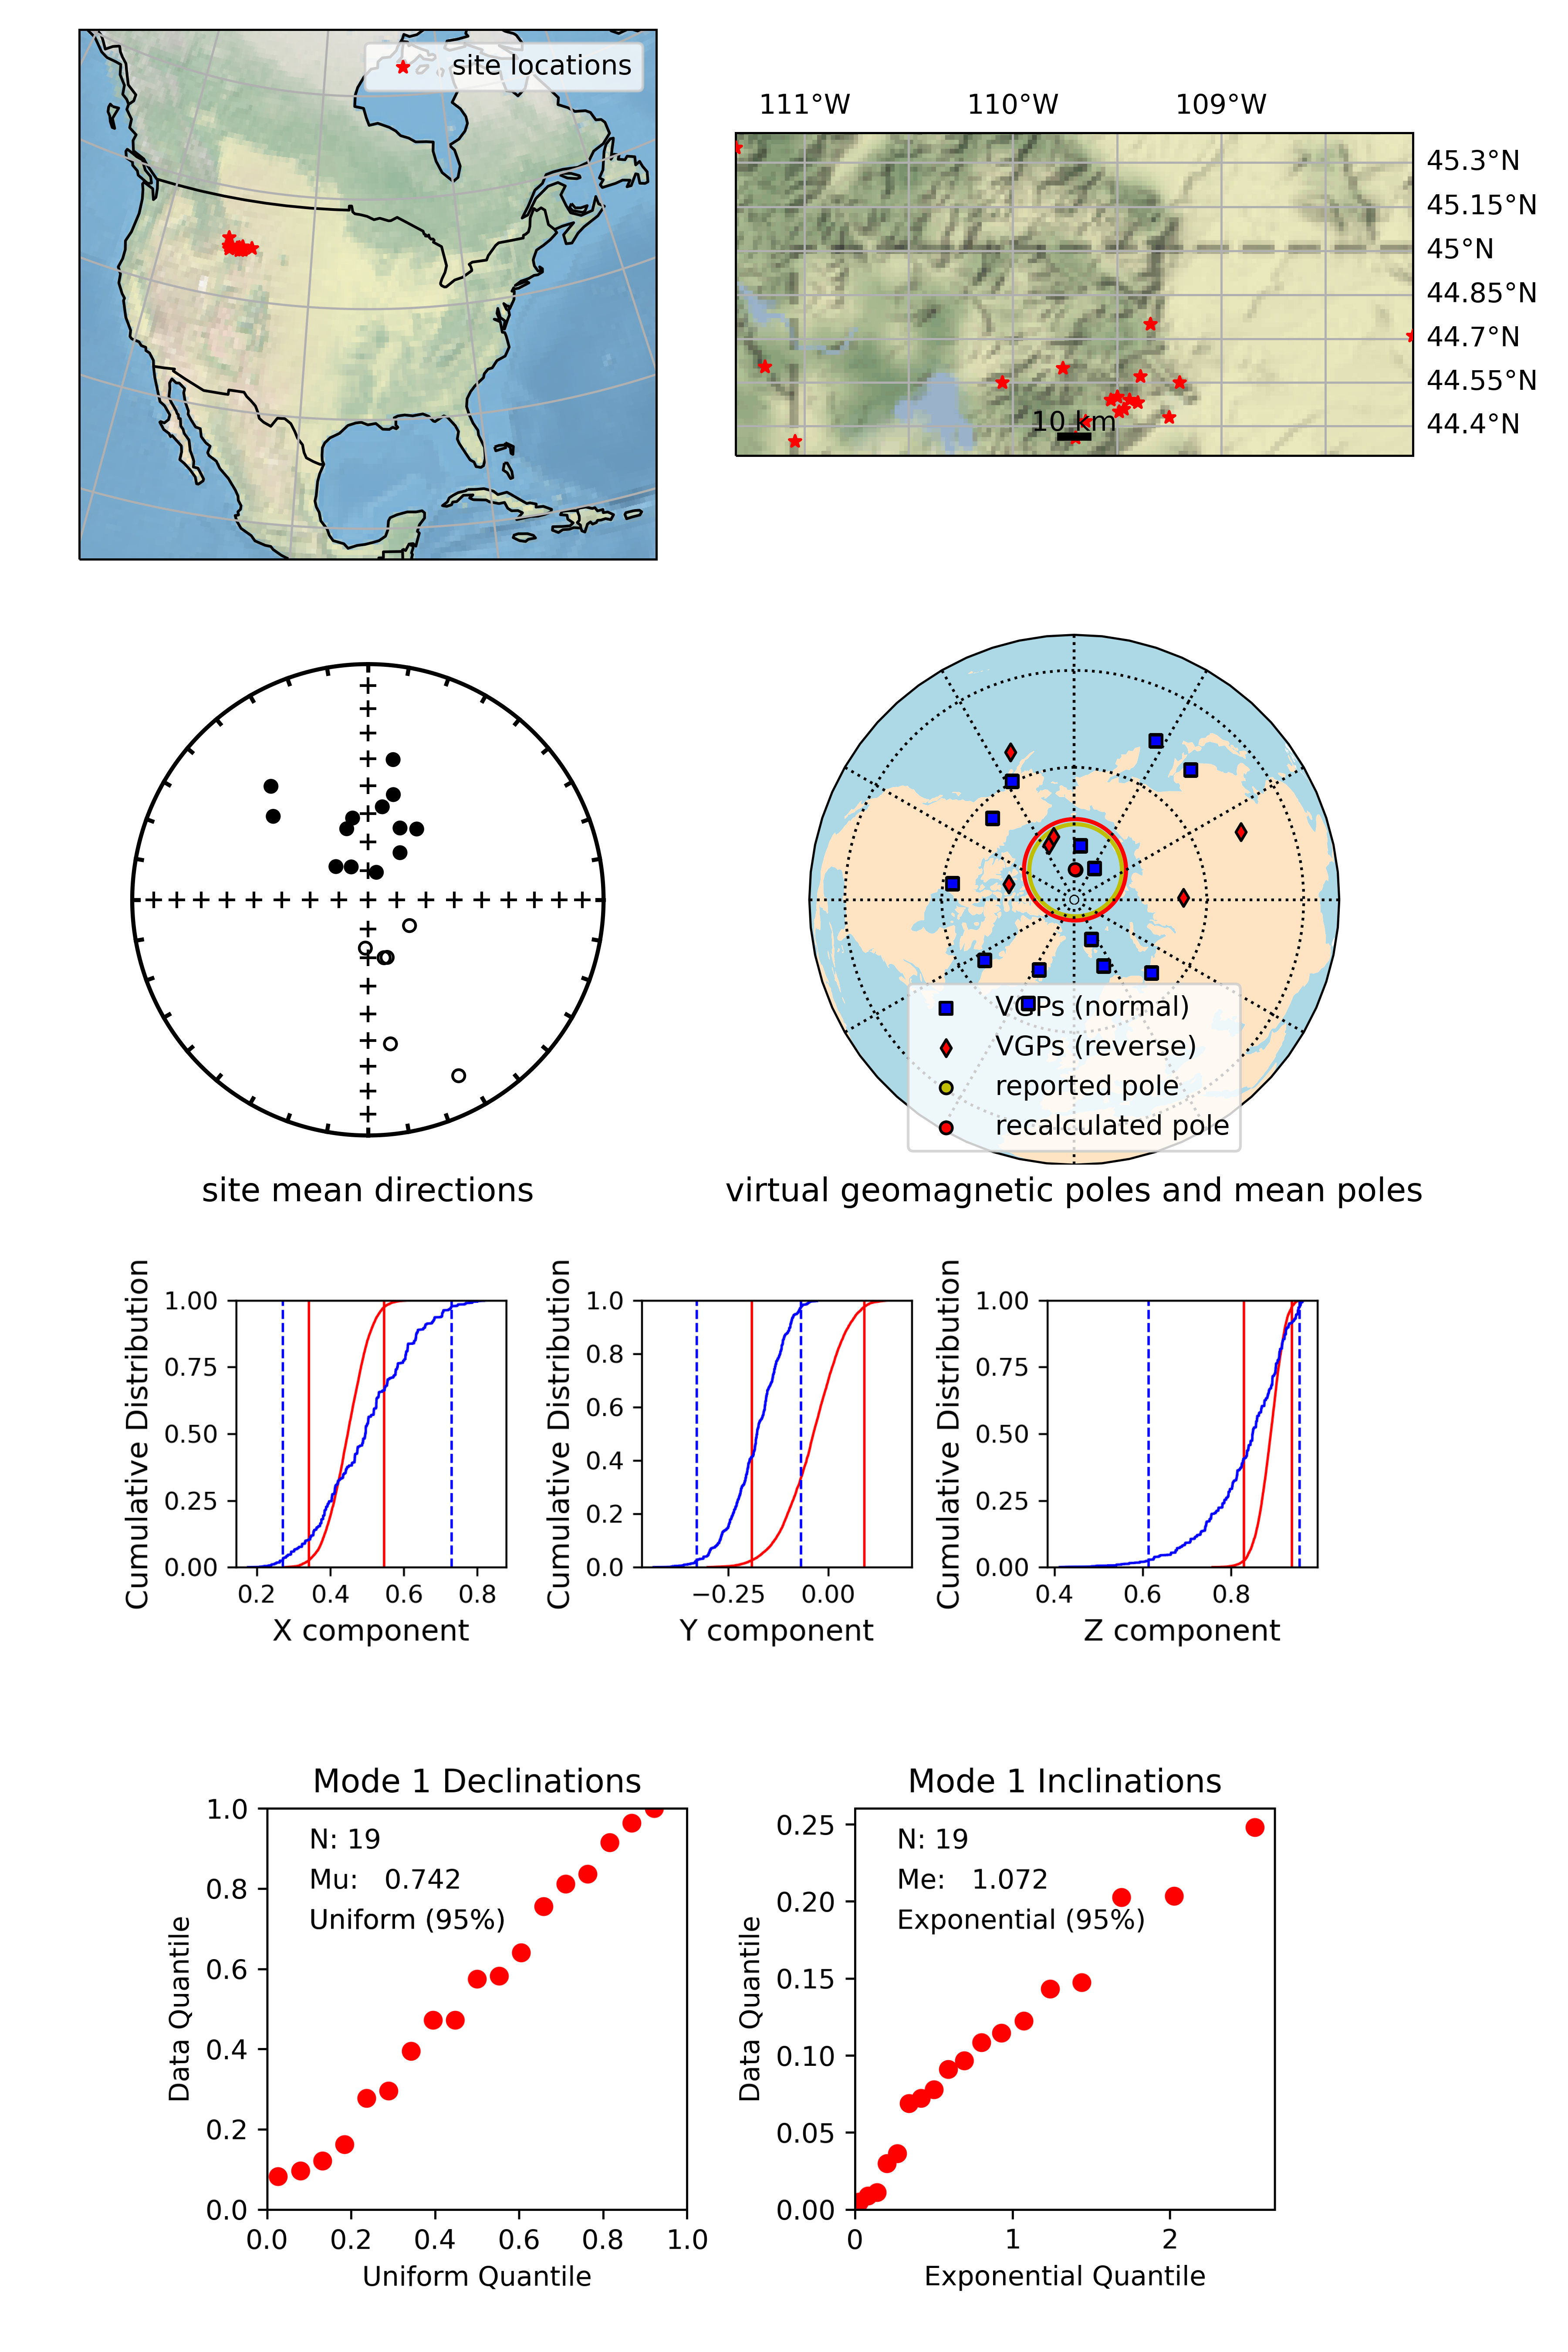
\includegraphics[width=5 in]{./15/1/pole_summary.png}
\caption{Summary of data from locality 15 (Absaroka volcanics) pole 1 (Shive and Pruss (1977)).}
\end{figure}

\subsection{Pole 2}
\begin{tabular}{lllll}
\toprule
{} &   N &  Plat &   Plon &  A95 \\
\midrule
Reported mean pole                                 &  33 &  88.0 &  265.5 &  5.0 \\
Mean pole (calculated from VGPs)                   &  33 &  87.9 &  270.8 &  5.1 \\
Mean pole (calculated from transformed directions) &  33 &  87.9 &  270.6 &  5.1 \\
\bottomrule
\end{tabular}

\begin{tabular}{ll}
\toprule
{} &                                                          result \\
\midrule
Bootstrap reversal test  &                                                            Pass \\
Parametric reversal test &  Pass (angle 3.1º below 11.5º critical angle); C classification \\
Bayesian reversal test   &                                   Common mean: positive support \\
Fisher Q-Q test          &                             Consistent with Fisher distribution \\
\bottomrule
\end{tabular}

\begin{figure}[H]
\centering
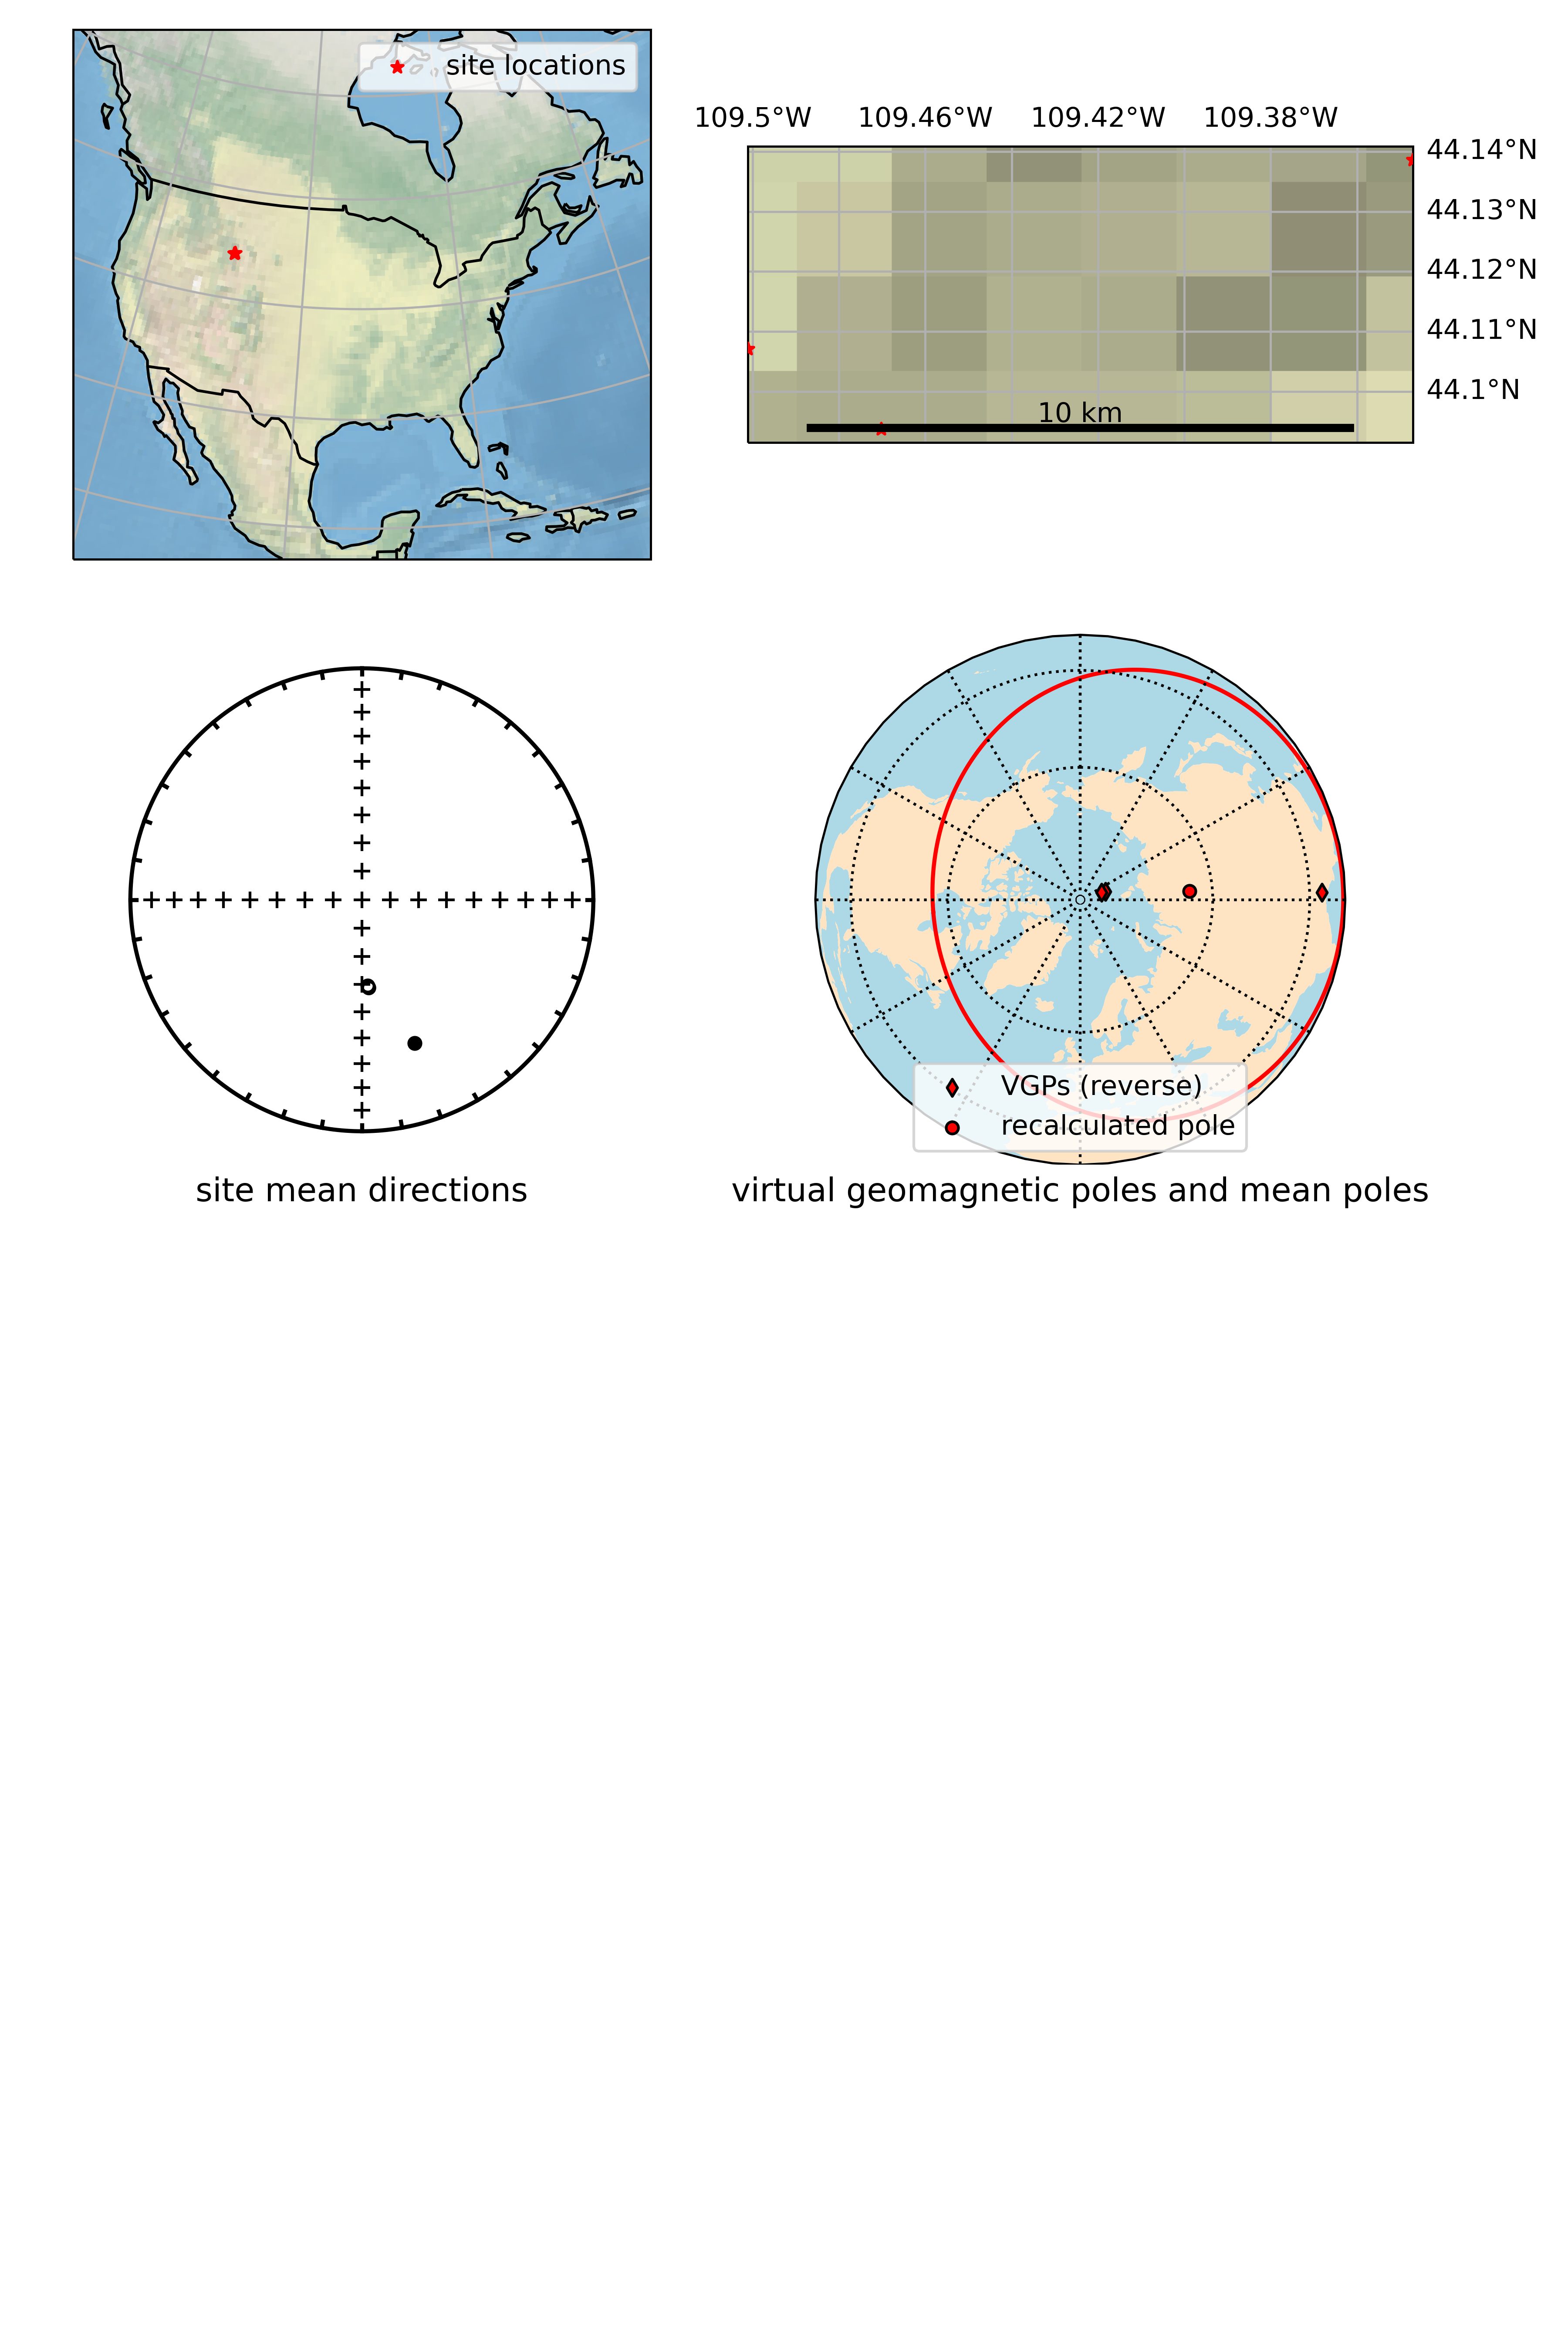
\includegraphics[width=5 in]{./15/2/pole_summary.png}
\caption{Summary of data from locality 15 (Absaroka volcanics) pole 2 (Re-calculated from Nyblade et al. (1986) [who didn't calculate a pole position]).}
\end{figure}

\subsection{Pole 3}
\begin{tabular}{lllll}
\toprule
{} &   N &  Plat &   Plon &  A95 \\
\midrule
Reported mean pole                                 &  33 &  88.0 &  265.5 &  5.0 \\
Mean pole (calculated from VGPs)                   &  33 &  87.9 &  270.8 &  5.1 \\
Mean pole (calculated from transformed directions) &  33 &  87.9 &  270.6 &  5.1 \\
\bottomrule
\end{tabular}

\begin{tabular}{ll}
\toprule
{} &                                                          result \\
\midrule
Bootstrap reversal test  &                                                            Pass \\
Parametric reversal test &  Pass (angle 3.1º below 11.5º critical angle); C classification \\
Bayesian reversal test   &                                   Common mean: positive support \\
Fisher Q-Q test          &                             Consistent with Fisher distribution \\
\bottomrule
\end{tabular}

\begin{figure}[H]
\centering
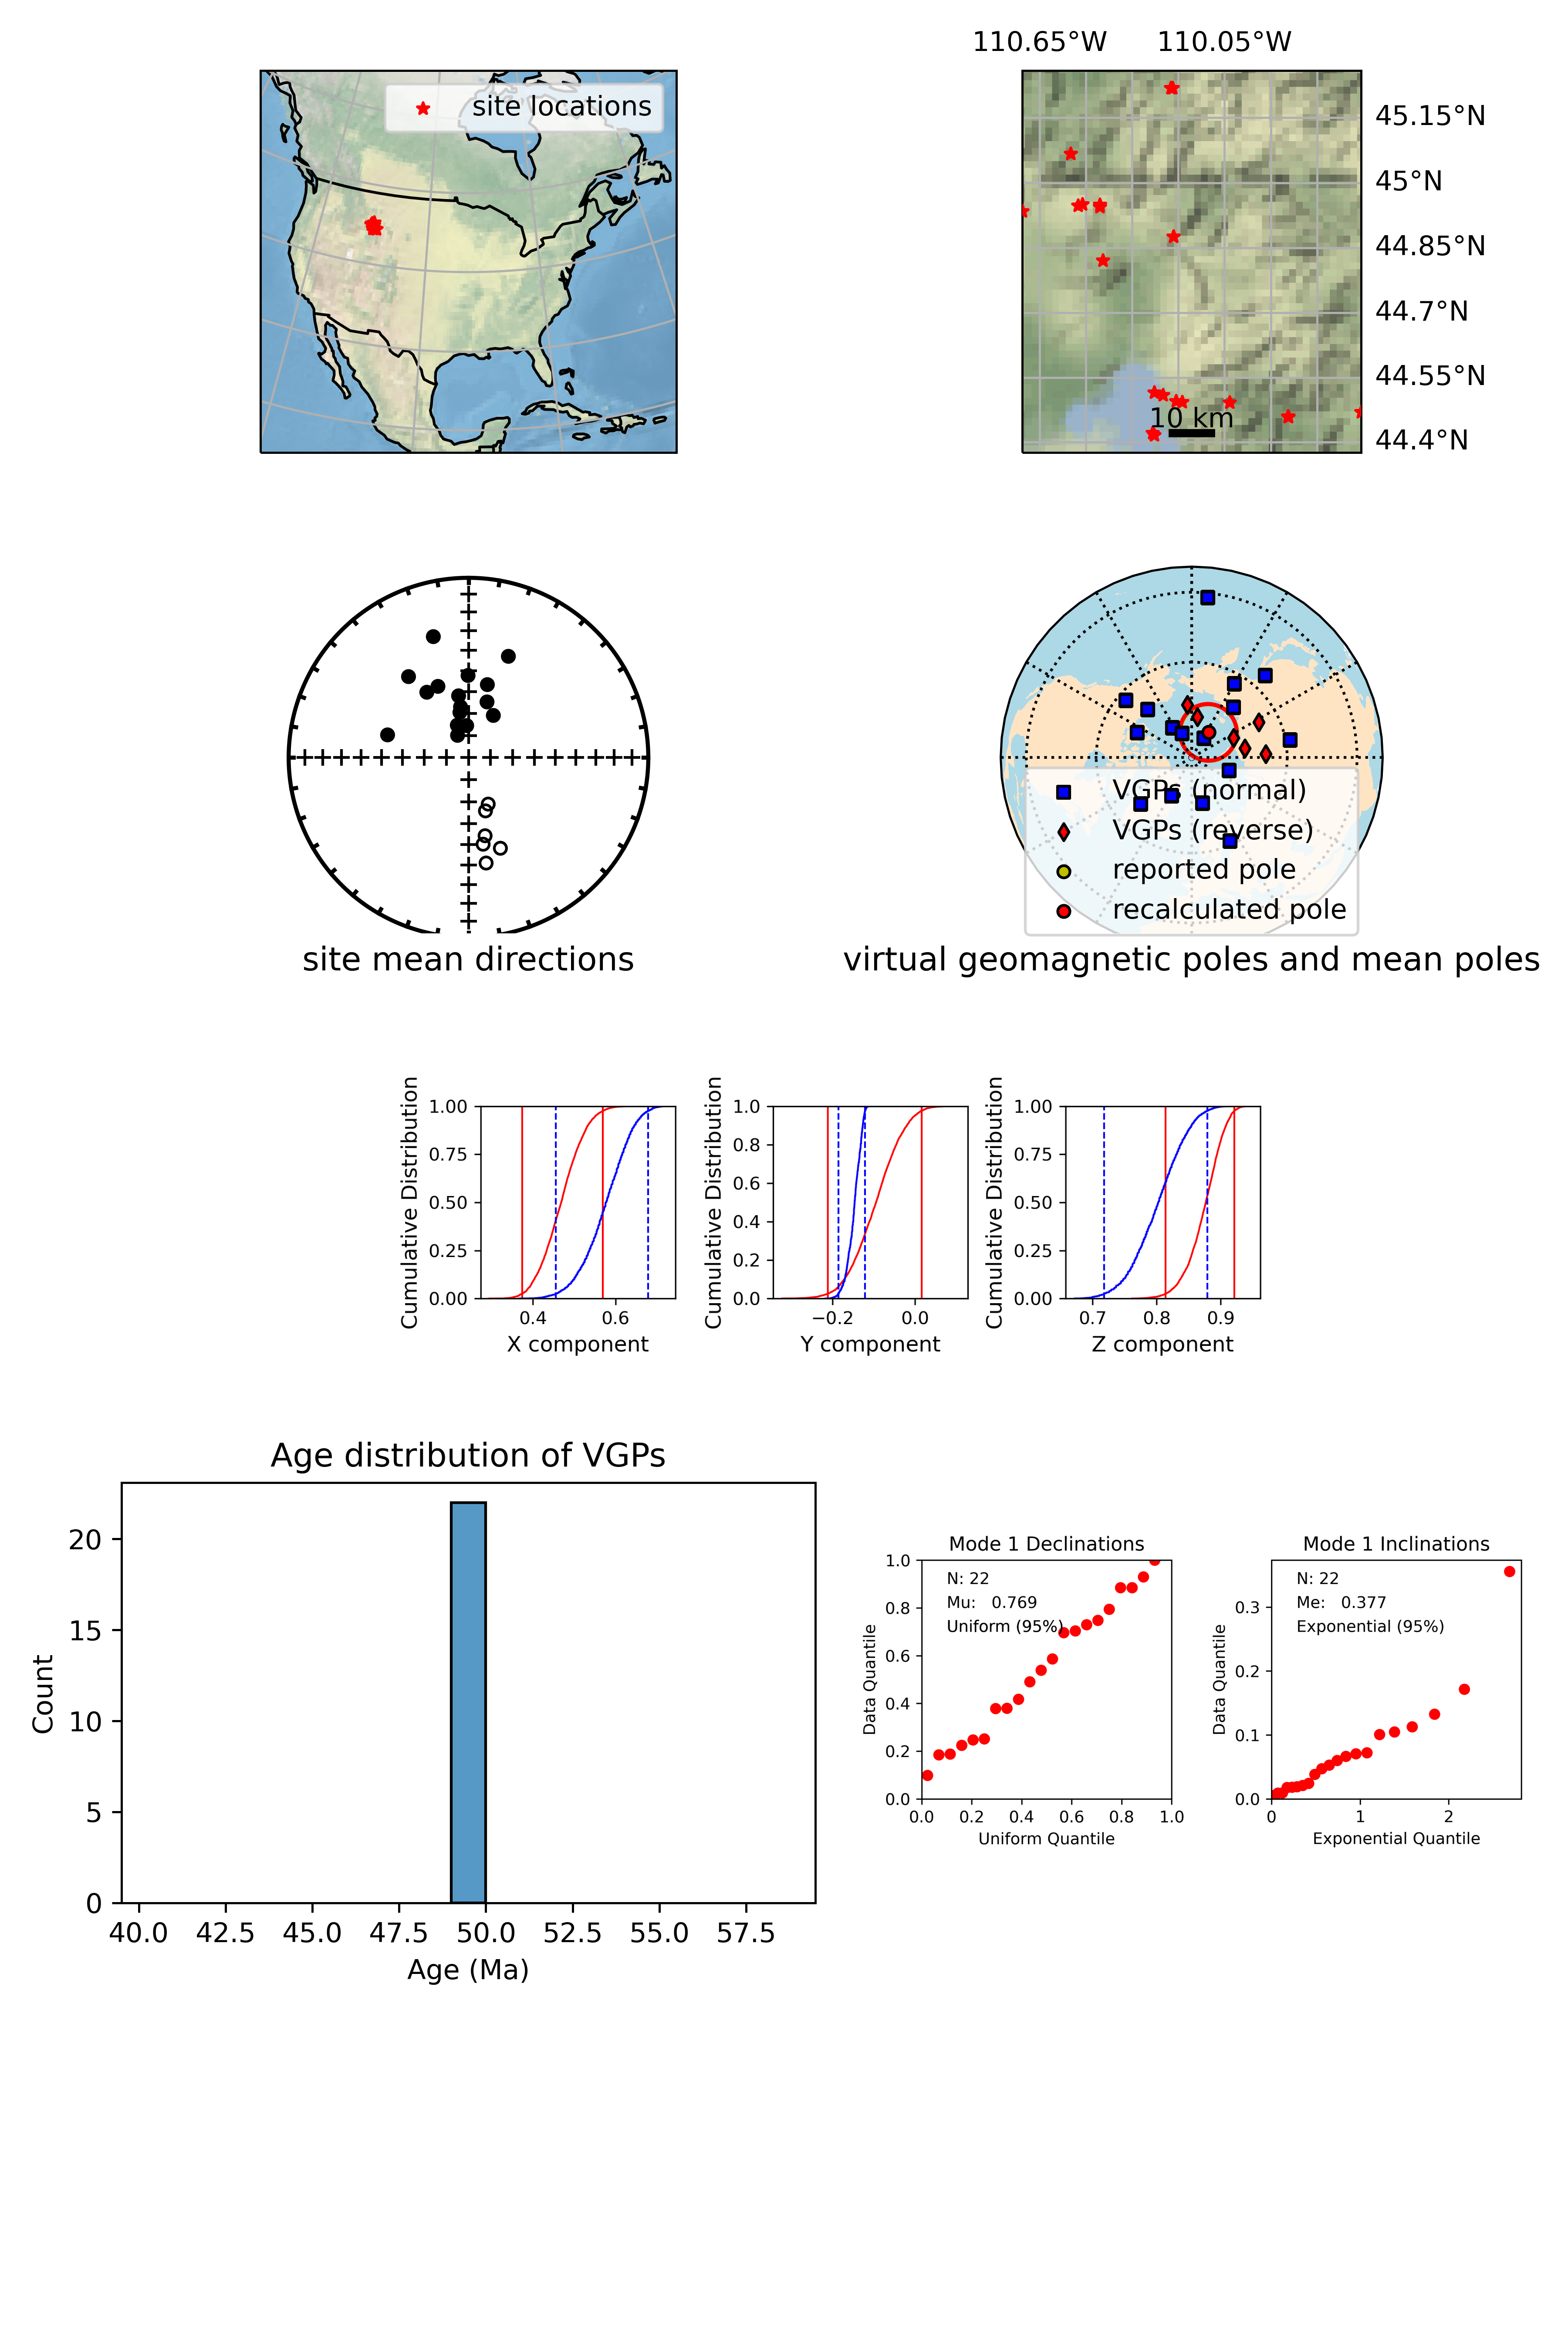
\includegraphics[width=5 in]{./15/3/pole_summary.png}
\caption{Summary of data from locality 15 (Absaroka volcanics) pole 3 (Harlan and Morgan (2010)).}
\end{figure}

\section{Eastern TMVB}
\subsection{Pole 1}
\begin{tabular}{lllll}
\toprule
{} &   N &  Plat &   Plon &  A95 \\
\midrule
Reported mean pole                                 &  33 &  88.0 &  265.5 &  5.0 \\
Mean pole (calculated from VGPs)                   &  33 &  87.9 &  270.8 &  5.1 \\
Mean pole (calculated from transformed directions) &  33 &  87.9 &  270.6 &  5.1 \\
\bottomrule
\end{tabular}

\begin{tabular}{ll}
\toprule
{} &                                                          result \\
\midrule
Bootstrap reversal test  &                                                            Pass \\
Parametric reversal test &  Pass (angle 3.1º below 11.5º critical angle); C classification \\
Bayesian reversal test   &                                   Common mean: positive support \\
Fisher Q-Q test          &                             Consistent with Fisher distribution \\
\bottomrule
\end{tabular}

\begin{figure}[H]
\centering
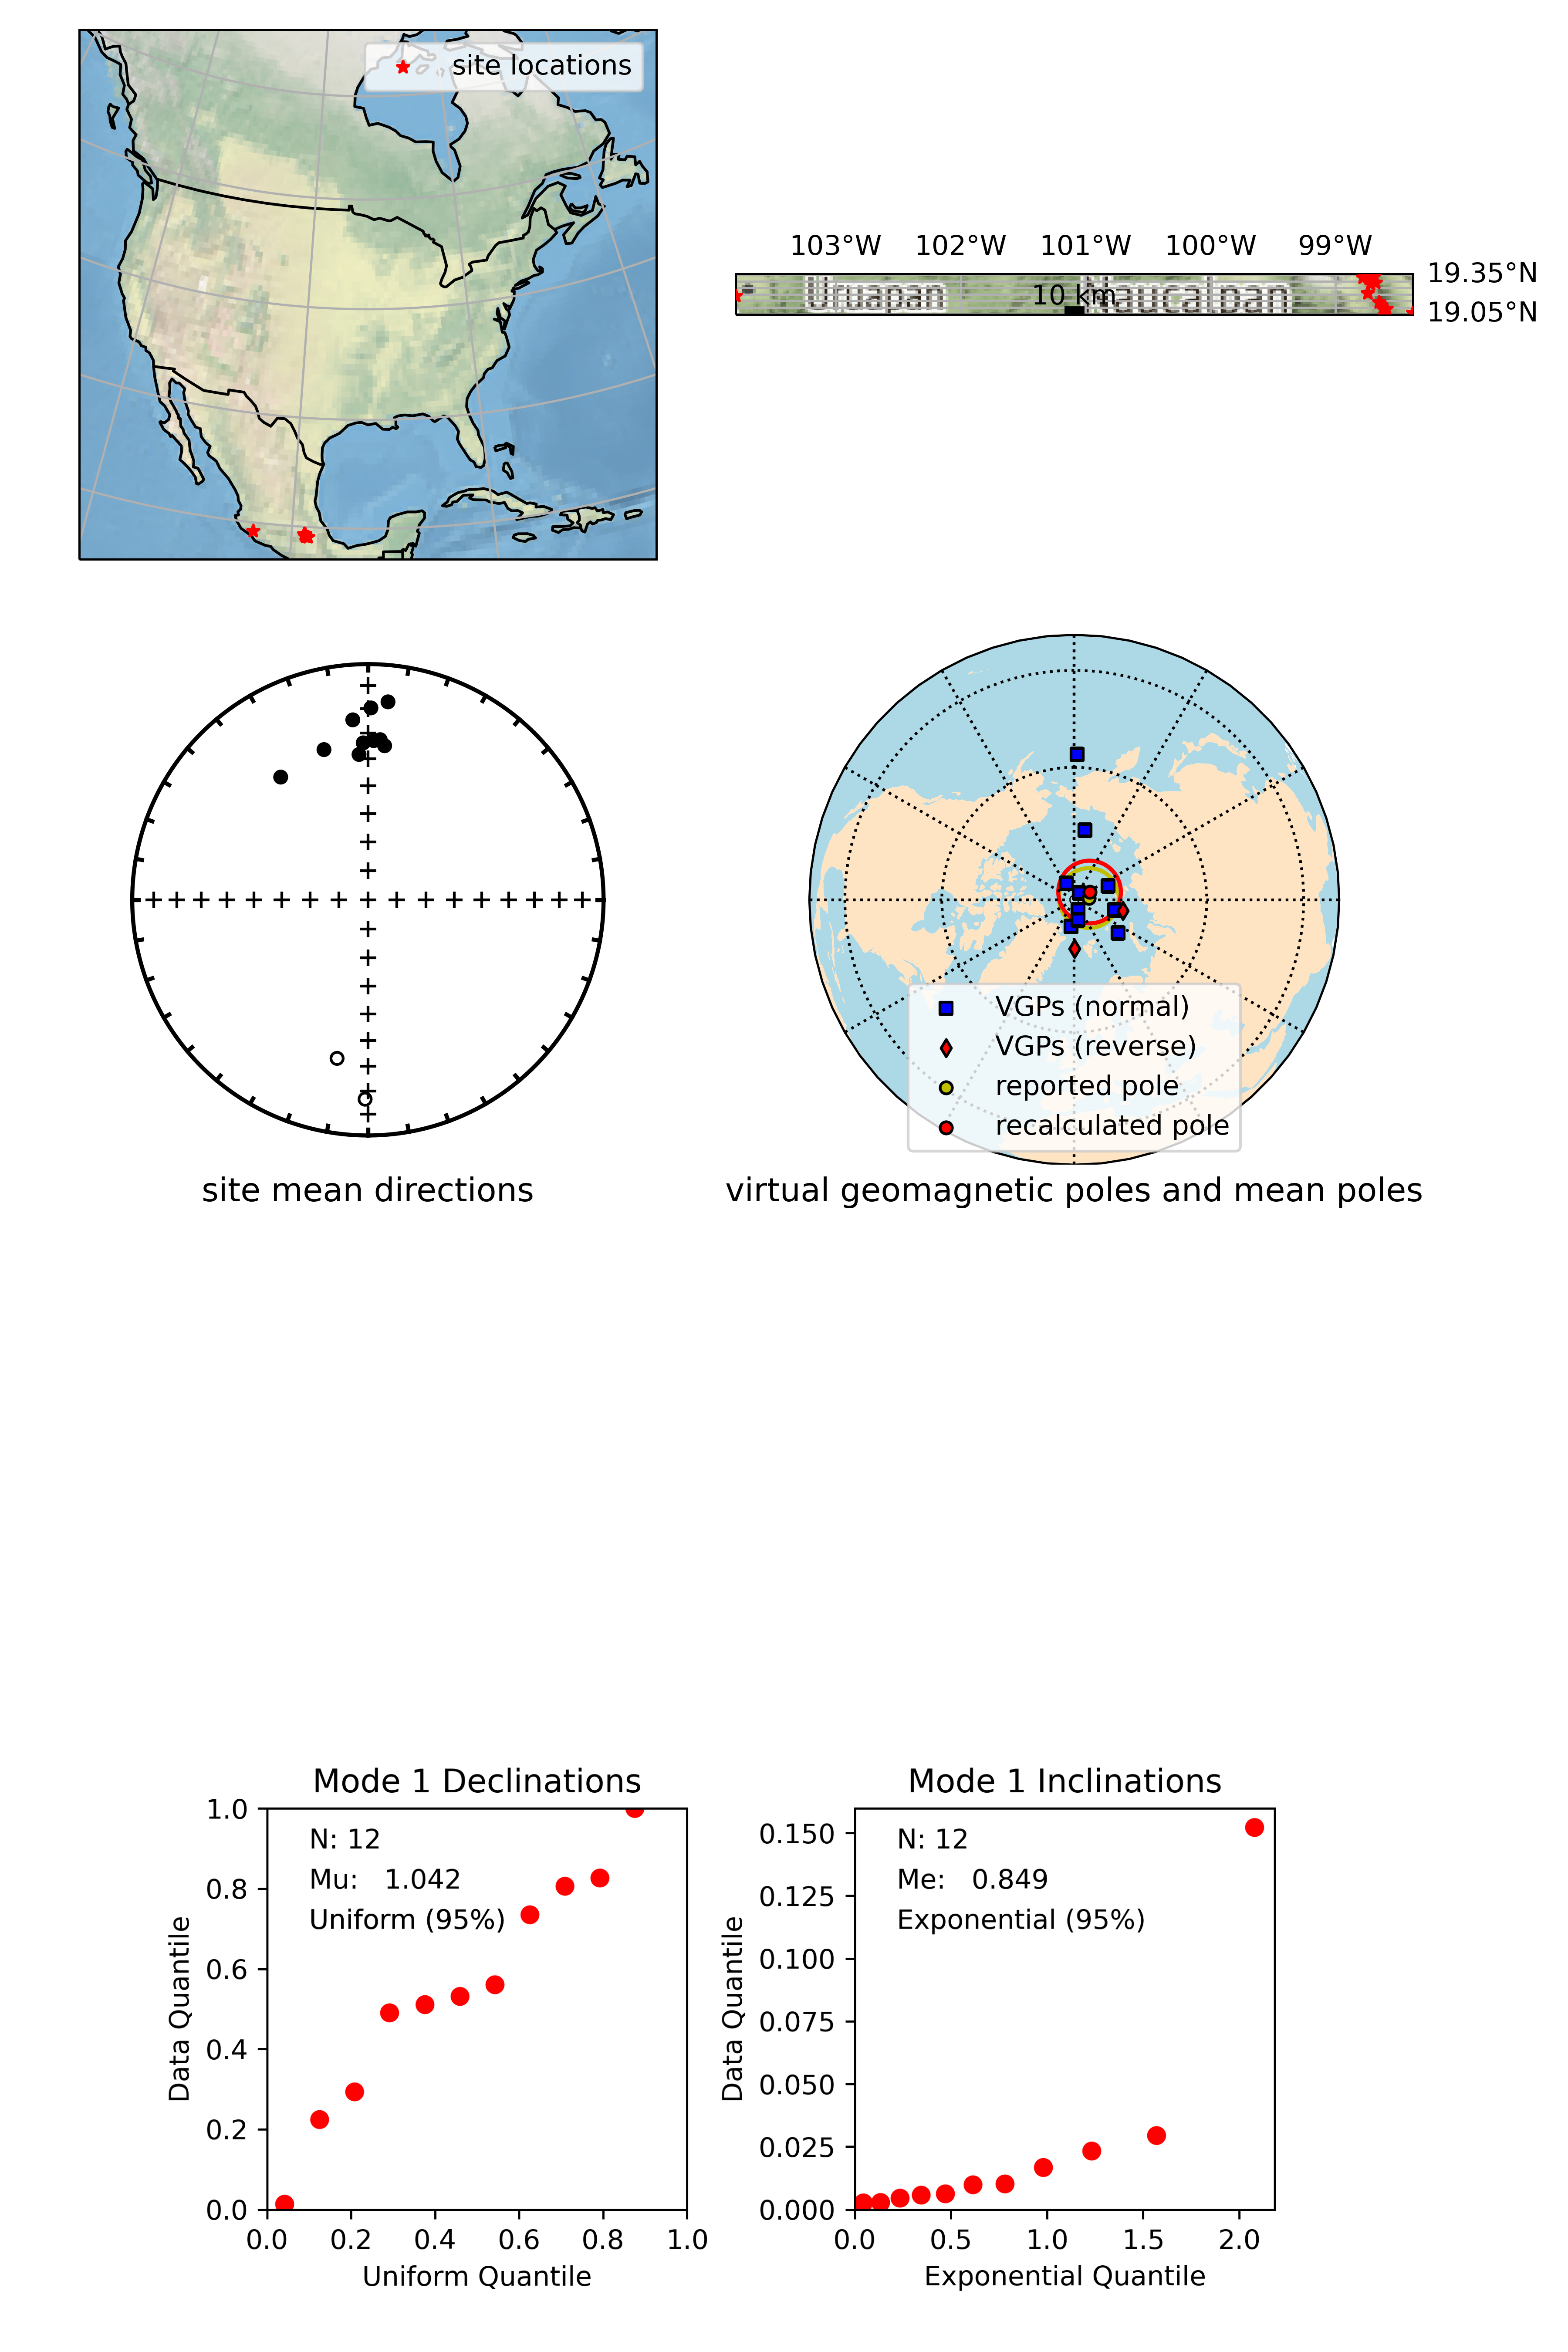
\includegraphics[width=5 in]{./16/1/pole_summary.png}
\caption{Summary of data from locality 16 (Eastern TMVB) pole 1 (Ruiz-Martínez et al. (2000)).}
\end{figure}

\subsection{Pole 2}
\begin{tabular}{lllll}
\toprule
{} &   N &  Plat &   Plon &  A95 \\
\midrule
Reported mean pole                                 &  33 &  88.0 &  265.5 &  5.0 \\
Mean pole (calculated from VGPs)                   &  33 &  87.9 &  270.8 &  5.1 \\
Mean pole (calculated from transformed directions) &  33 &  87.9 &  270.6 &  5.1 \\
\bottomrule
\end{tabular}

\begin{tabular}{ll}
\toprule
{} &                                                          result \\
\midrule
Bootstrap reversal test  &                                                            Pass \\
Parametric reversal test &  Pass (angle 3.1º below 11.5º critical angle); C classification \\
Bayesian reversal test   &                                   Common mean: positive support \\
Fisher Q-Q test          &                             Consistent with Fisher distribution \\
\bottomrule
\end{tabular}

\begin{figure}[H]
\centering
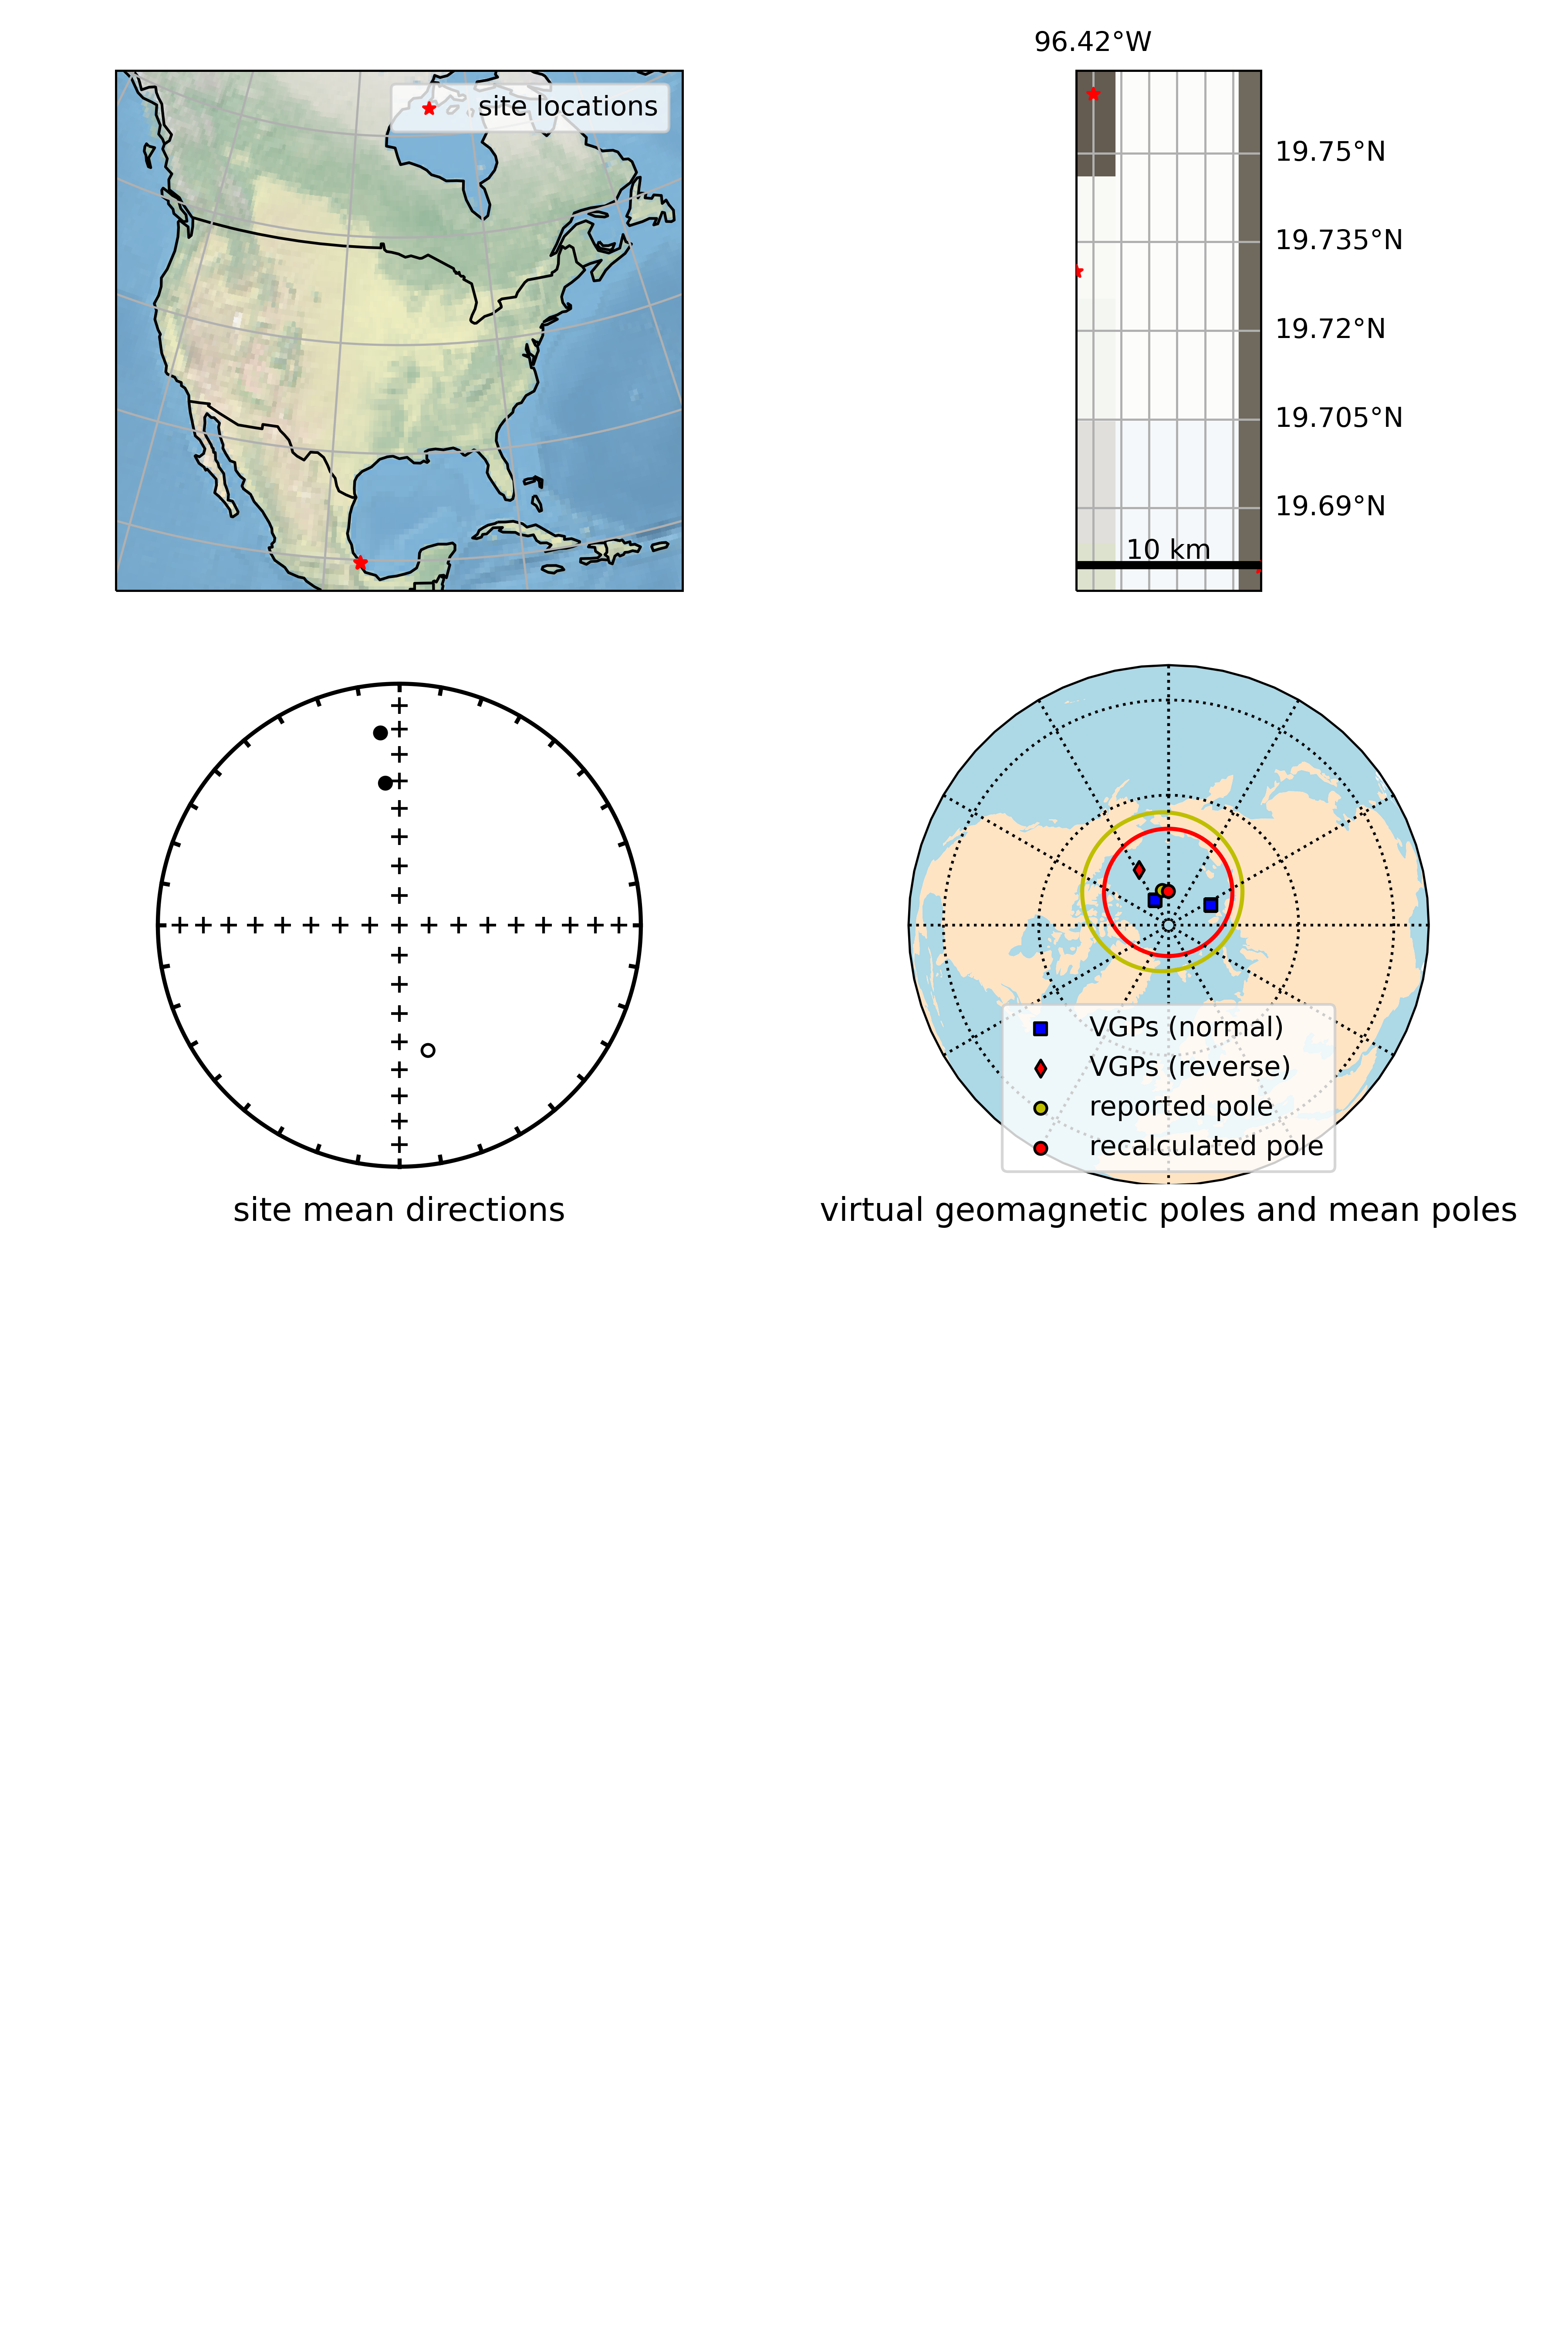
\includegraphics[width=5 in]{./16/2/pole_summary.png}
\caption{Summary of data from locality 16 (Eastern TMVB) pole 2 (Ruiz-Martínez et al. (2000)).}
\end{figure}

\subsection{Pole 3}
\begin{tabular}{lllll}
\toprule
{} &   N &  Plat &   Plon &  A95 \\
\midrule
Reported mean pole                                 &  33 &  88.0 &  265.5 &  5.0 \\
Mean pole (calculated from VGPs)                   &  33 &  87.9 &  270.8 &  5.1 \\
Mean pole (calculated from transformed directions) &  33 &  87.9 &  270.6 &  5.1 \\
\bottomrule
\end{tabular}

\begin{tabular}{ll}
\toprule
{} &                                                          result \\
\midrule
Bootstrap reversal test  &                                                            Pass \\
Parametric reversal test &  Pass (angle 3.1º below 11.5º critical angle); C classification \\
Bayesian reversal test   &                                   Common mean: positive support \\
Fisher Q-Q test          &                             Consistent with Fisher distribution \\
\bottomrule
\end{tabular}

\begin{figure}[H]
\centering
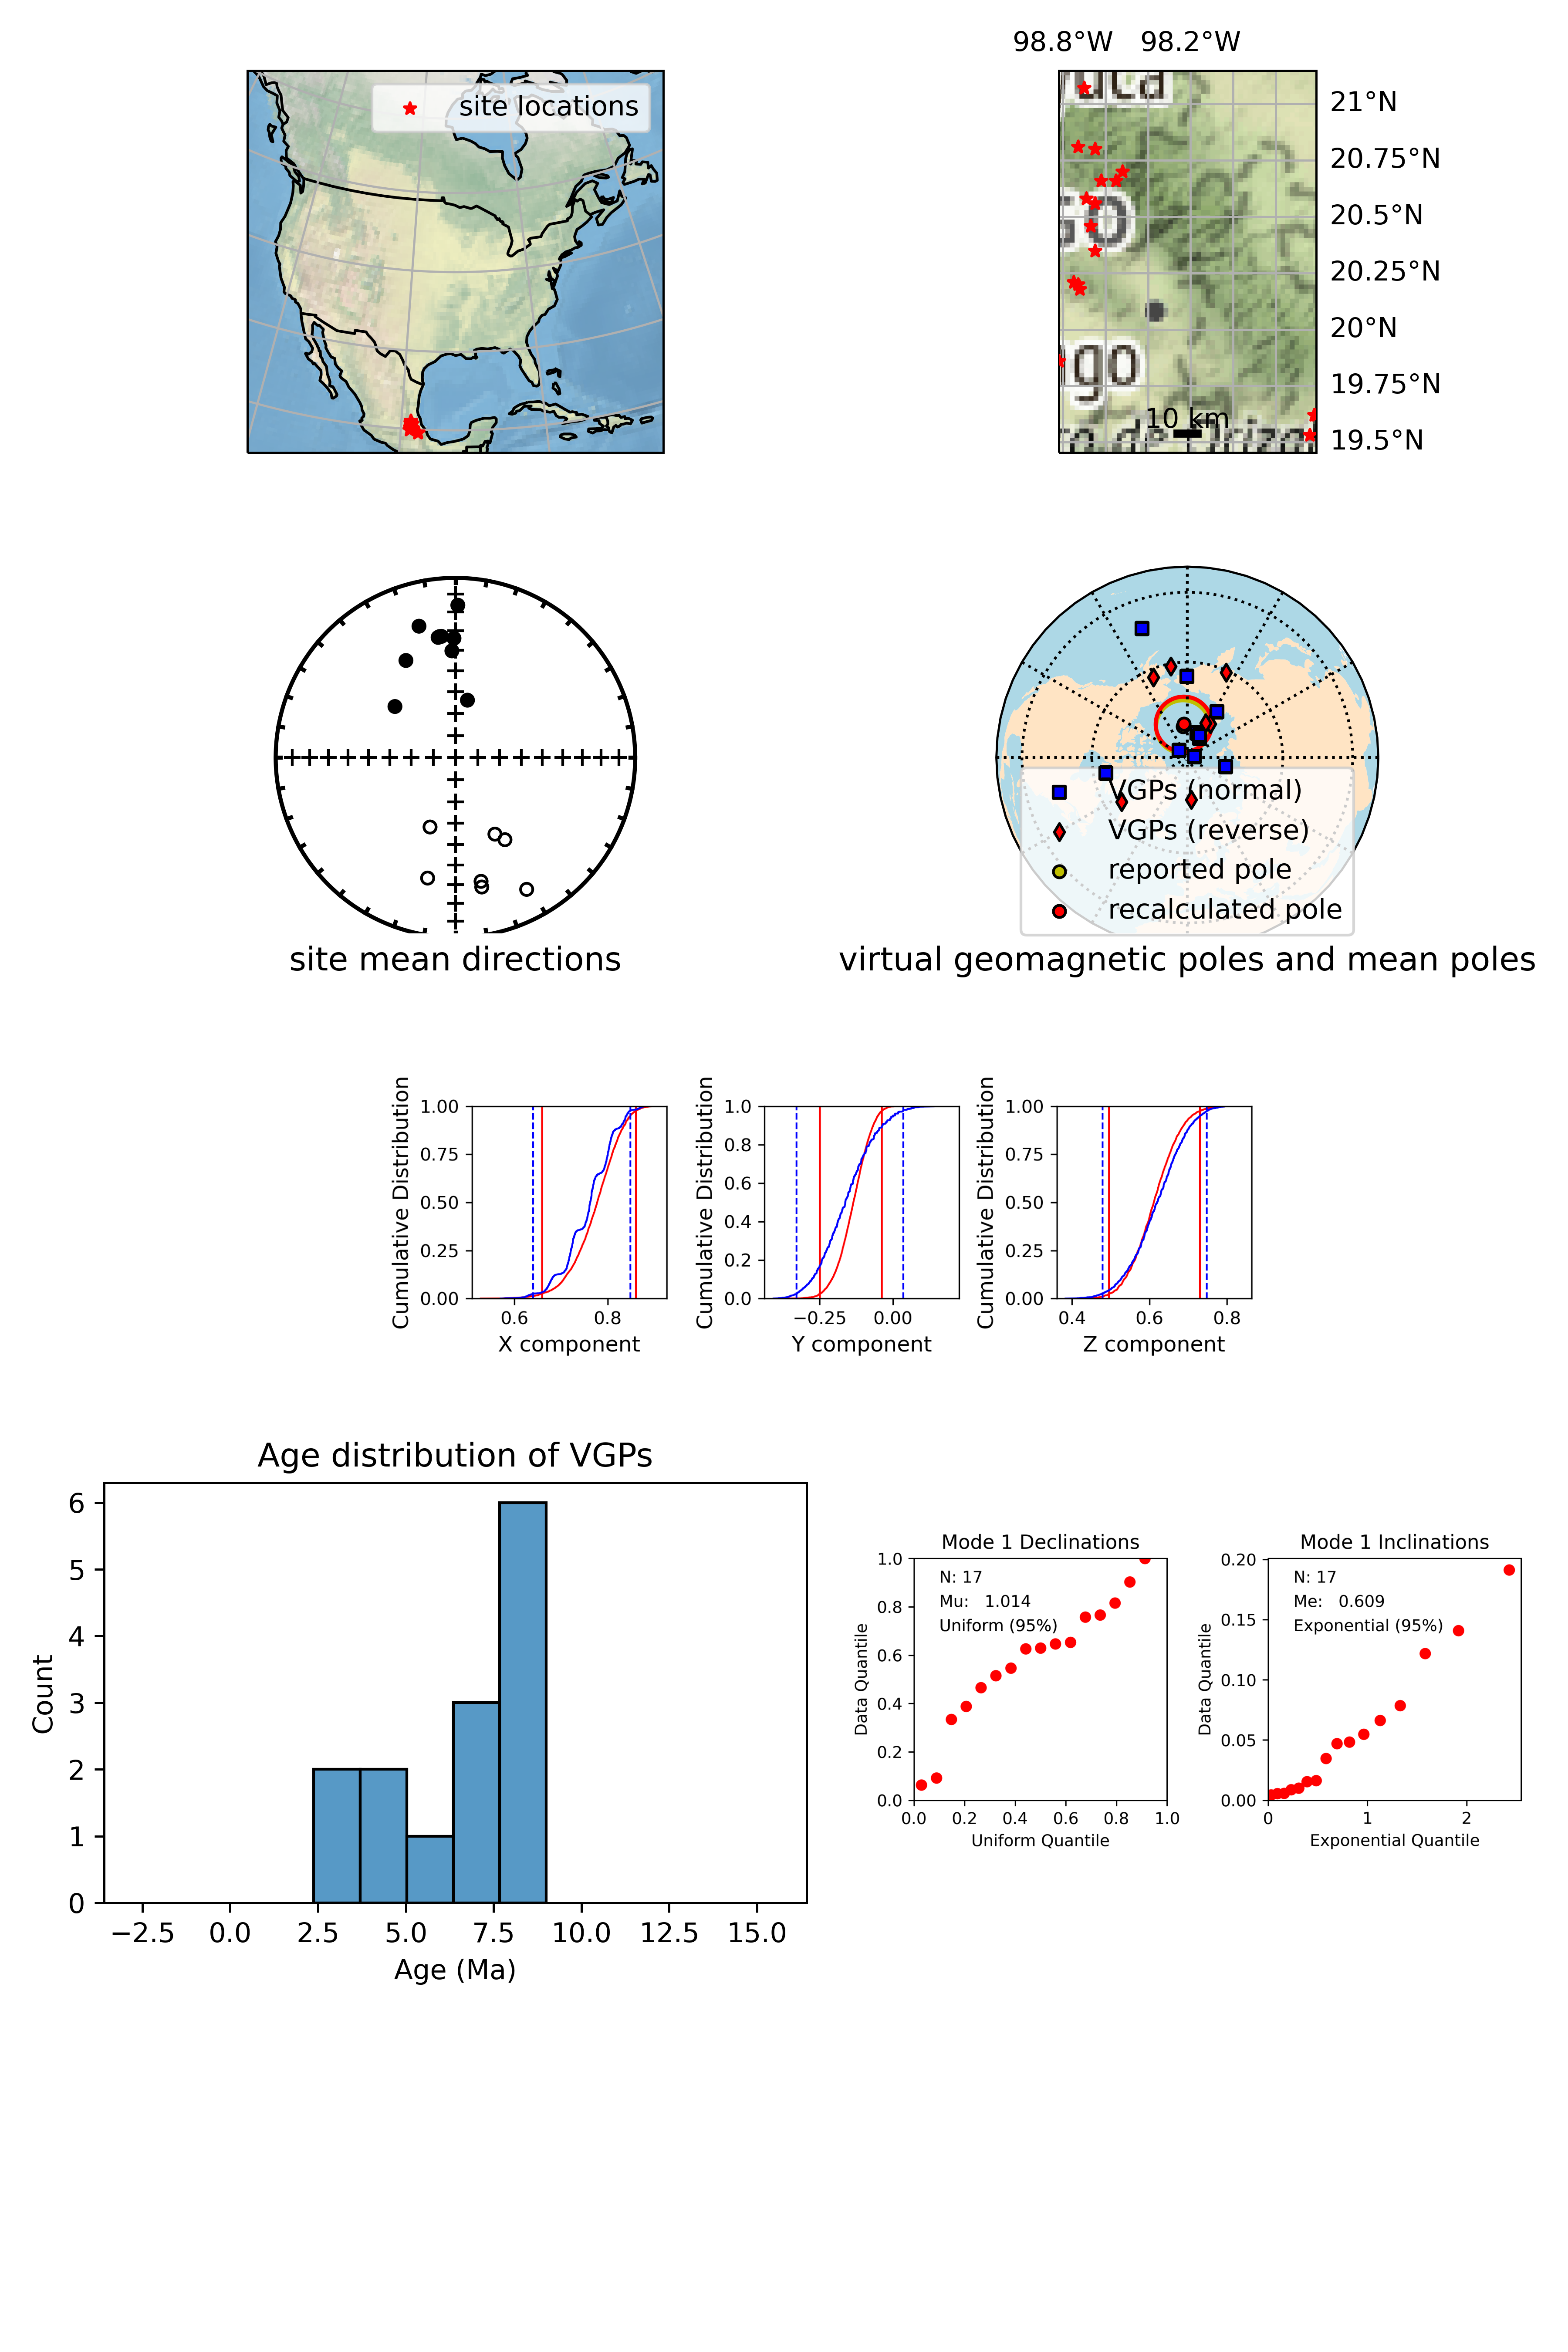
\includegraphics[width=5 in]{./16/3/pole_summary.png}
\caption{Summary of data from locality 16 (Eastern TMVB) pole 3 (Ruiz-Martínez et al. (2000)).}
\end{figure}

\section{Bishop tuff}
\subsection{Pole 1}
\begin{tabular}{lllll}
\toprule
{} &   N &  Plat &   Plon &  A95 \\
\midrule
Reported mean pole                                 &  33 &  88.0 &  265.5 &  5.0 \\
Mean pole (calculated from VGPs)                   &  33 &  87.9 &  270.8 &  5.1 \\
Mean pole (calculated from transformed directions) &  33 &  87.9 &  270.6 &  5.1 \\
\bottomrule
\end{tabular}

\begin{tabular}{ll}
\toprule
{} &                                                          result \\
\midrule
Bootstrap reversal test  &                                                            Pass \\
Parametric reversal test &  Pass (angle 3.1º below 11.5º critical angle); C classification \\
Bayesian reversal test   &                                   Common mean: positive support \\
Fisher Q-Q test          &                             Consistent with Fisher distribution \\
\bottomrule
\end{tabular}

\begin{figure}[H]
\centering
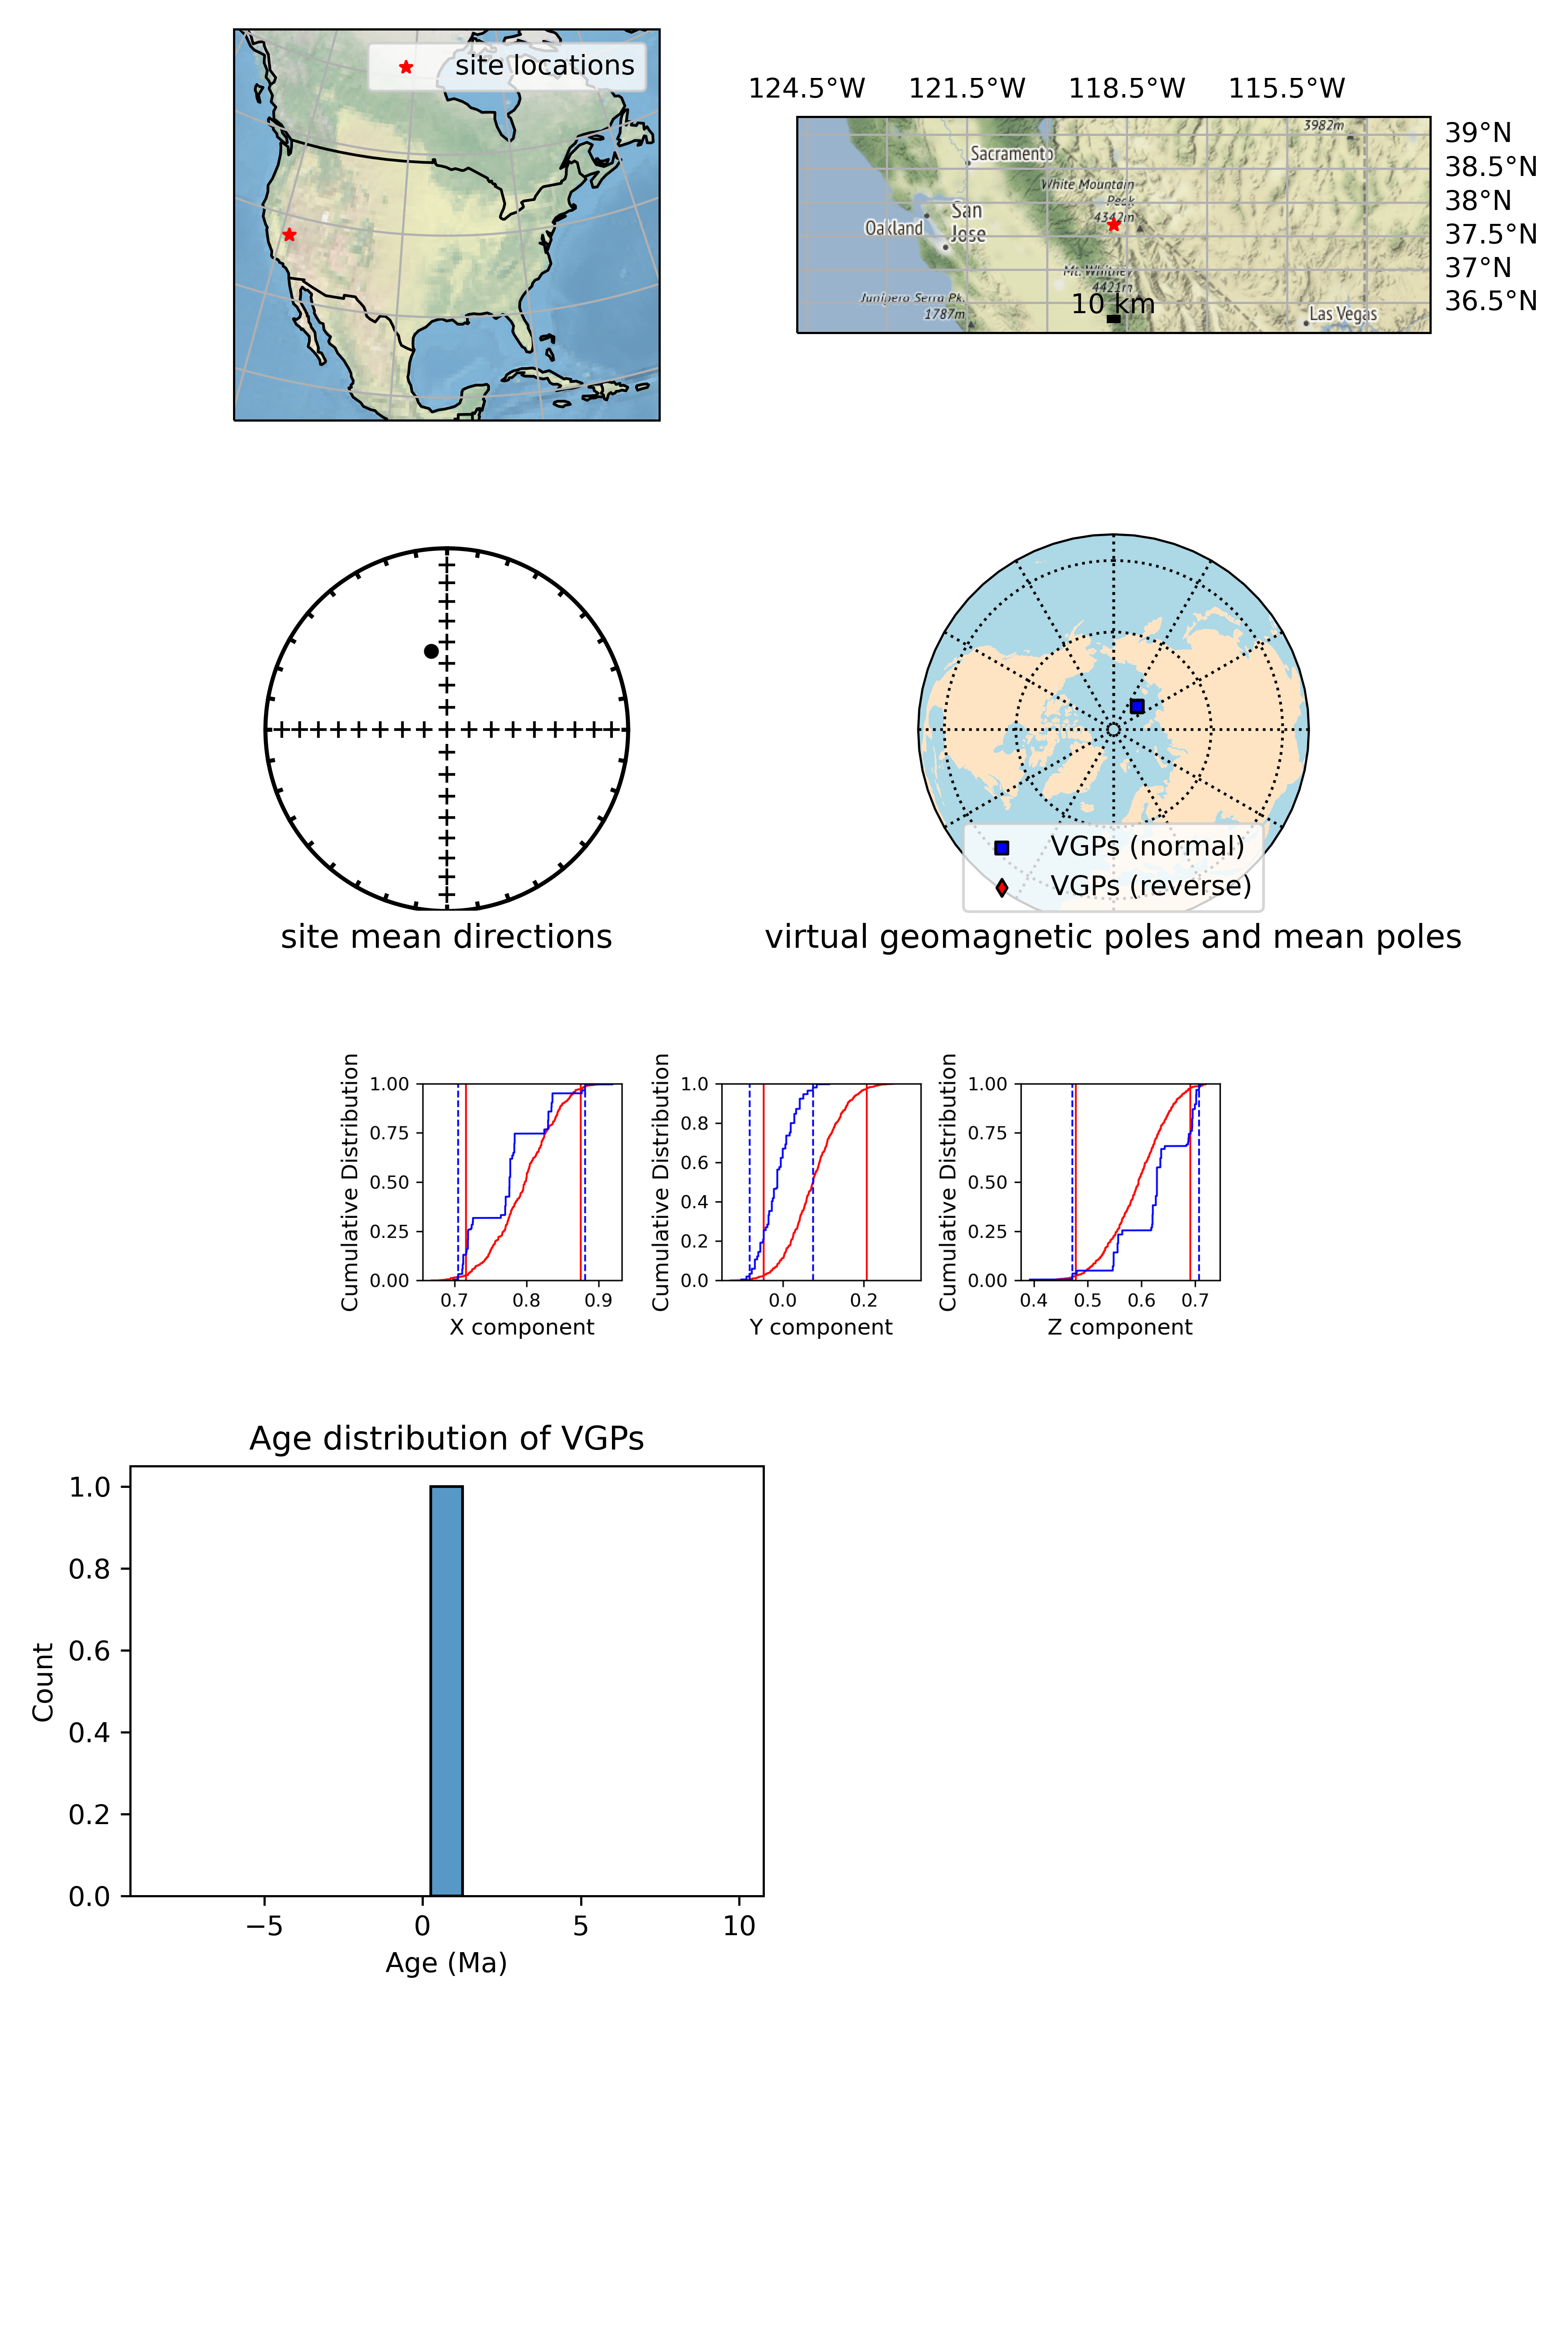
\includegraphics[width=5 in]{./17/1/pole_summary.png}
\caption{Summary of data from locality 17 (Bishop tuff) pole 1 (Palmer et al. (1996)).}
\end{figure}

\section{Western Central TMVB}
\subsection{Pole 1}
\begin{tabular}{lllll}
\toprule
{} &   N &  Plat &   Plon &  A95 \\
\midrule
Reported mean pole                                 &  33 &  88.0 &  265.5 &  5.0 \\
Mean pole (calculated from VGPs)                   &  33 &  87.9 &  270.8 &  5.1 \\
Mean pole (calculated from transformed directions) &  33 &  87.9 &  270.6 &  5.1 \\
\bottomrule
\end{tabular}

\begin{tabular}{ll}
\toprule
{} &                                                          result \\
\midrule
Bootstrap reversal test  &                                                            Pass \\
Parametric reversal test &  Pass (angle 3.1º below 11.5º critical angle); C classification \\
Bayesian reversal test   &                                   Common mean: positive support \\
Fisher Q-Q test          &                             Consistent with Fisher distribution \\
\bottomrule
\end{tabular}

\begin{figure}[H]
\centering
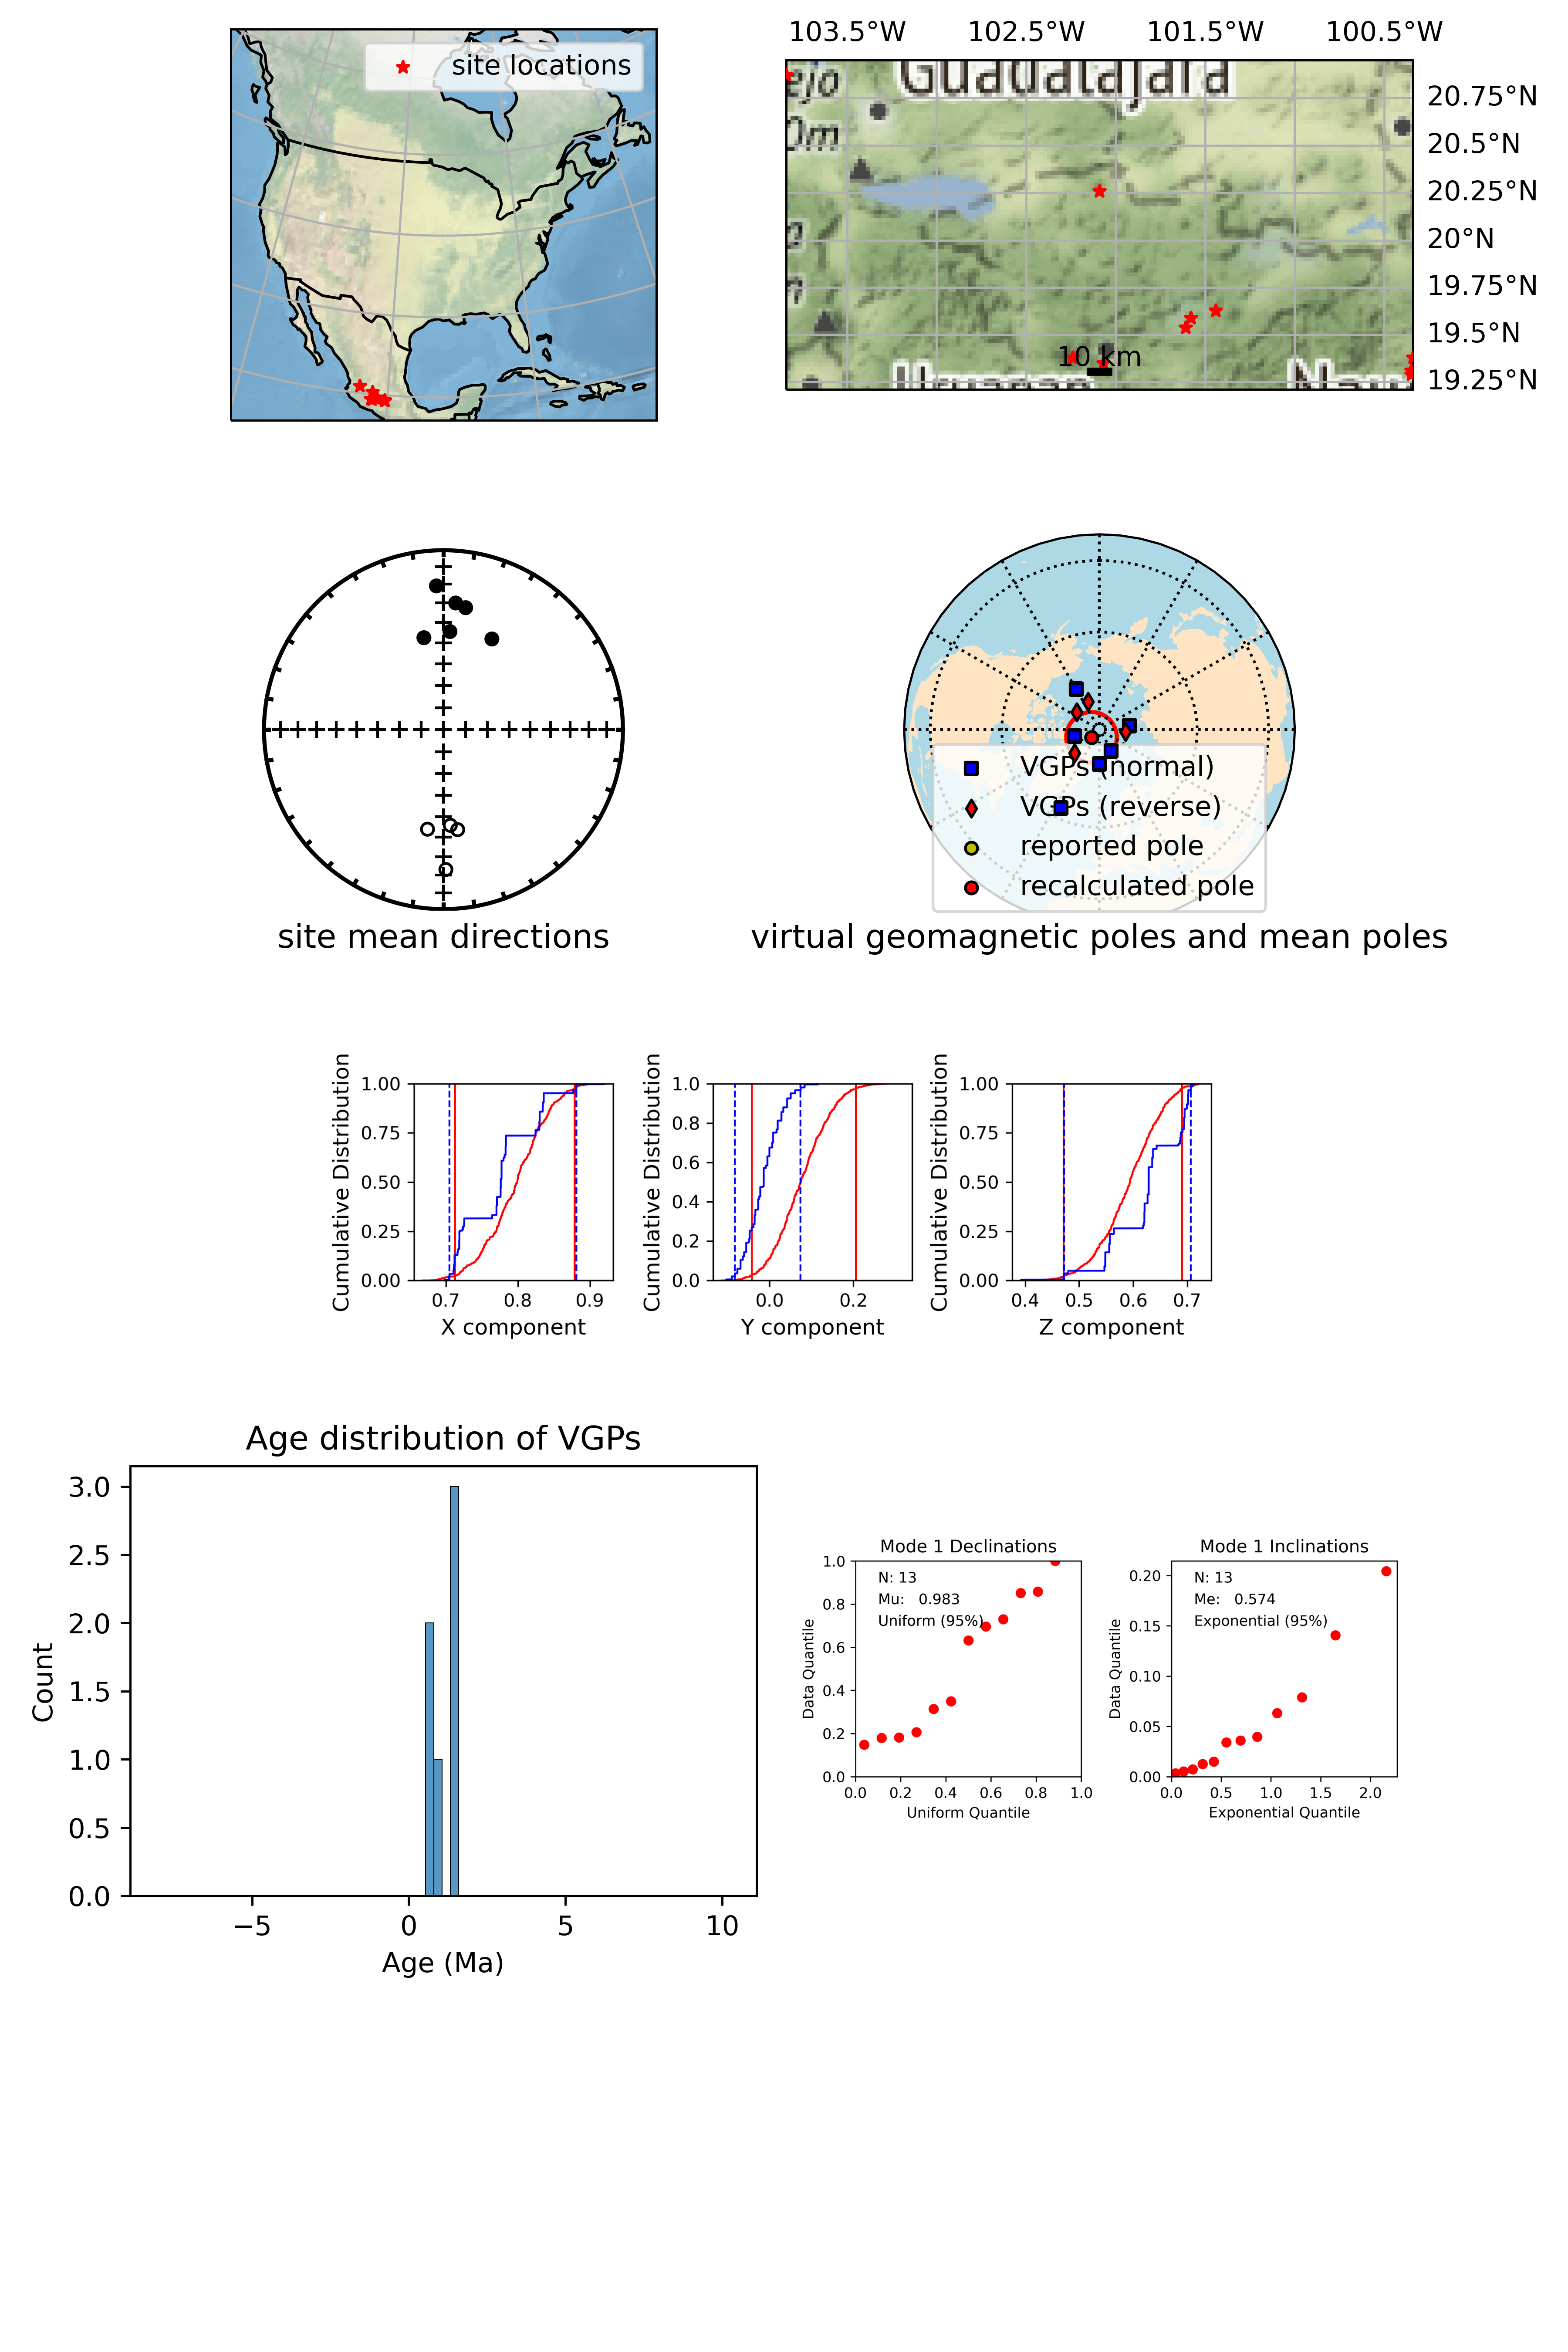
\includegraphics[width=5 in]{./18/1/pole_summary.png}
\caption{Summary of data from locality 18 (Western Central TMVB) pole 1 (Ruiz-Martínez et al. (2010)).}
\end{figure}

\subsection{Pole 2}
\begin{tabular}{lllll}
\toprule
{} &   N &  Plat &   Plon &  A95 \\
\midrule
Reported mean pole                                 &  33 &  88.0 &  265.5 &  5.0 \\
Mean pole (calculated from VGPs)                   &  33 &  87.9 &  270.8 &  5.1 \\
Mean pole (calculated from transformed directions) &  33 &  87.9 &  270.6 &  5.1 \\
\bottomrule
\end{tabular}

\begin{tabular}{ll}
\toprule
{} &                                                          result \\
\midrule
Bootstrap reversal test  &                                                            Pass \\
Parametric reversal test &  Pass (angle 3.1º below 11.5º critical angle); C classification \\
Bayesian reversal test   &                                   Common mean: positive support \\
Fisher Q-Q test          &                             Consistent with Fisher distribution \\
\bottomrule
\end{tabular}

\begin{figure}[H]
\centering
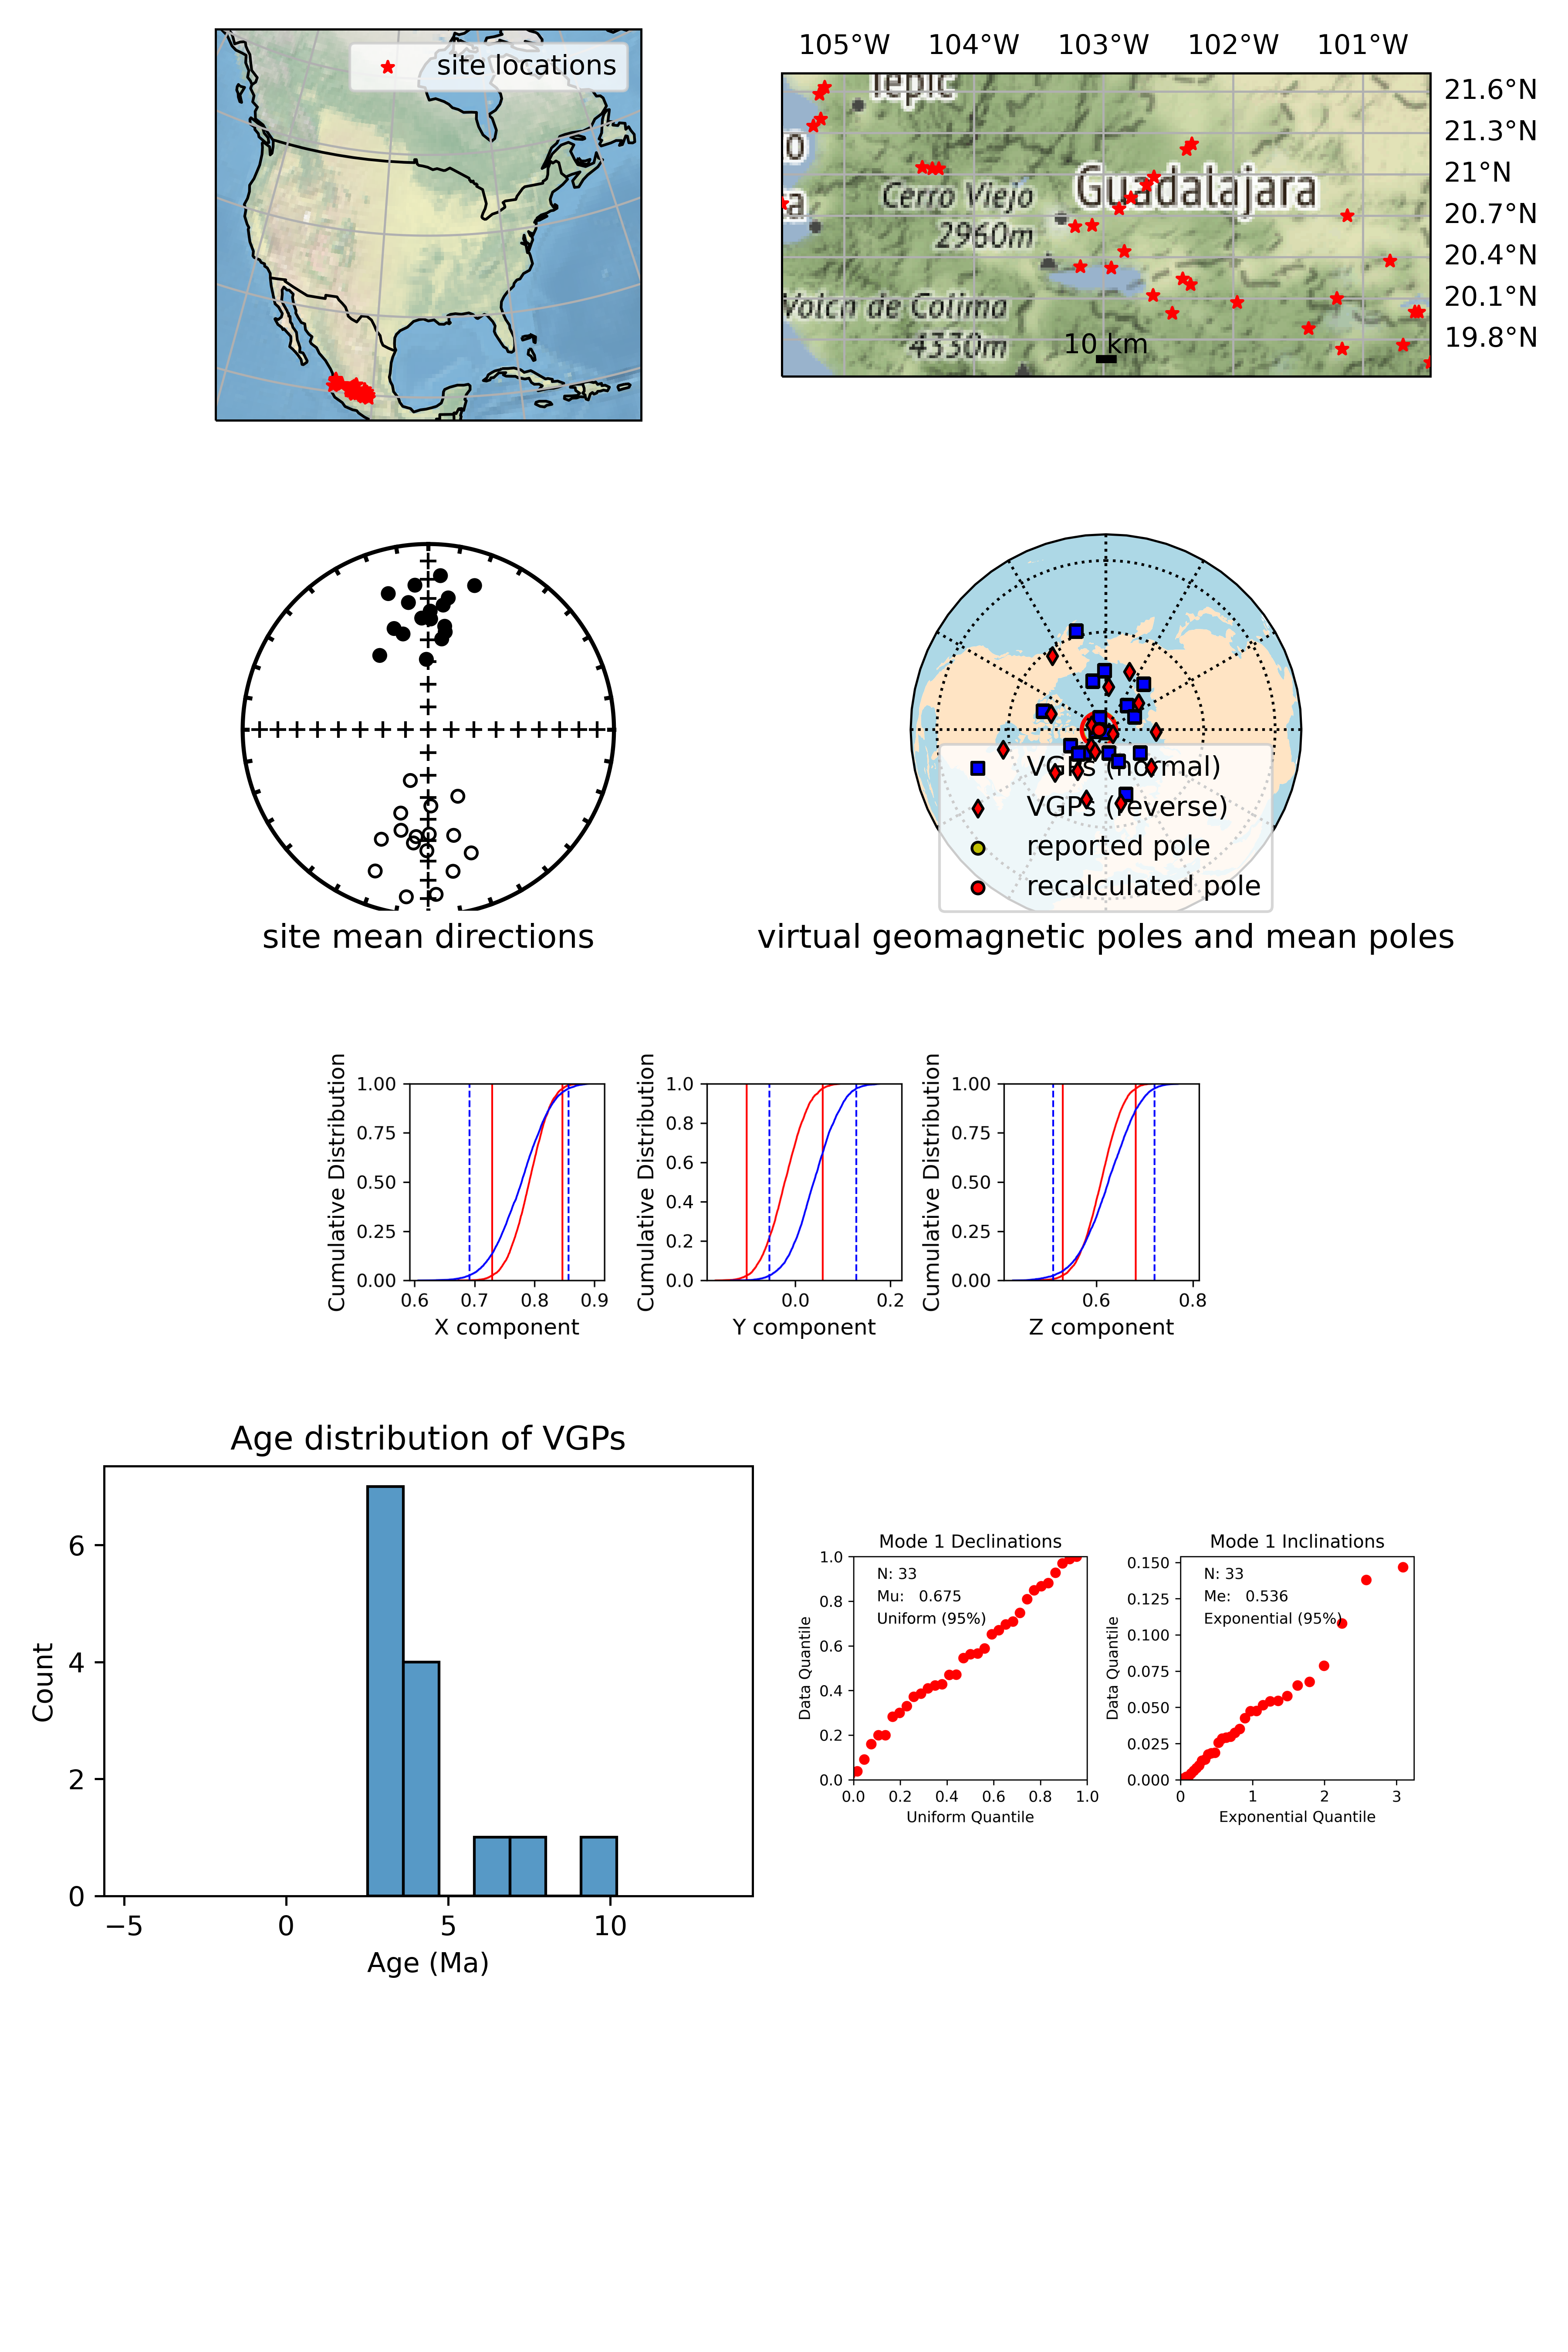
\includegraphics[width=5 in]{./18/2/pole_summary.png}
\caption{Summary of data from locality 18 (Western Central TMVB) pole 2 (Ruiz-Martínez et al. (2010)).}
\end{figure}

\section{Dinan Bay lavas}
\subsection{Pole 1}
\begin{tabular}{lllll}
\toprule
{} &   N &  Plat &   Plon &  A95 \\
\midrule
Reported mean pole                                 &  33 &  88.0 &  265.5 &  5.0 \\
Mean pole (calculated from VGPs)                   &  33 &  87.9 &  270.8 &  5.1 \\
Mean pole (calculated from transformed directions) &  33 &  87.9 &  270.6 &  5.1 \\
\bottomrule
\end{tabular}

\begin{tabular}{ll}
\toprule
{} &                                                          result \\
\midrule
Bootstrap reversal test  &                                                            Pass \\
Parametric reversal test &  Pass (angle 3.1º below 11.5º critical angle); C classification \\
Bayesian reversal test   &                                   Common mean: positive support \\
Fisher Q-Q test          &                             Consistent with Fisher distribution \\
\bottomrule
\end{tabular}

\begin{figure}[H]
\centering
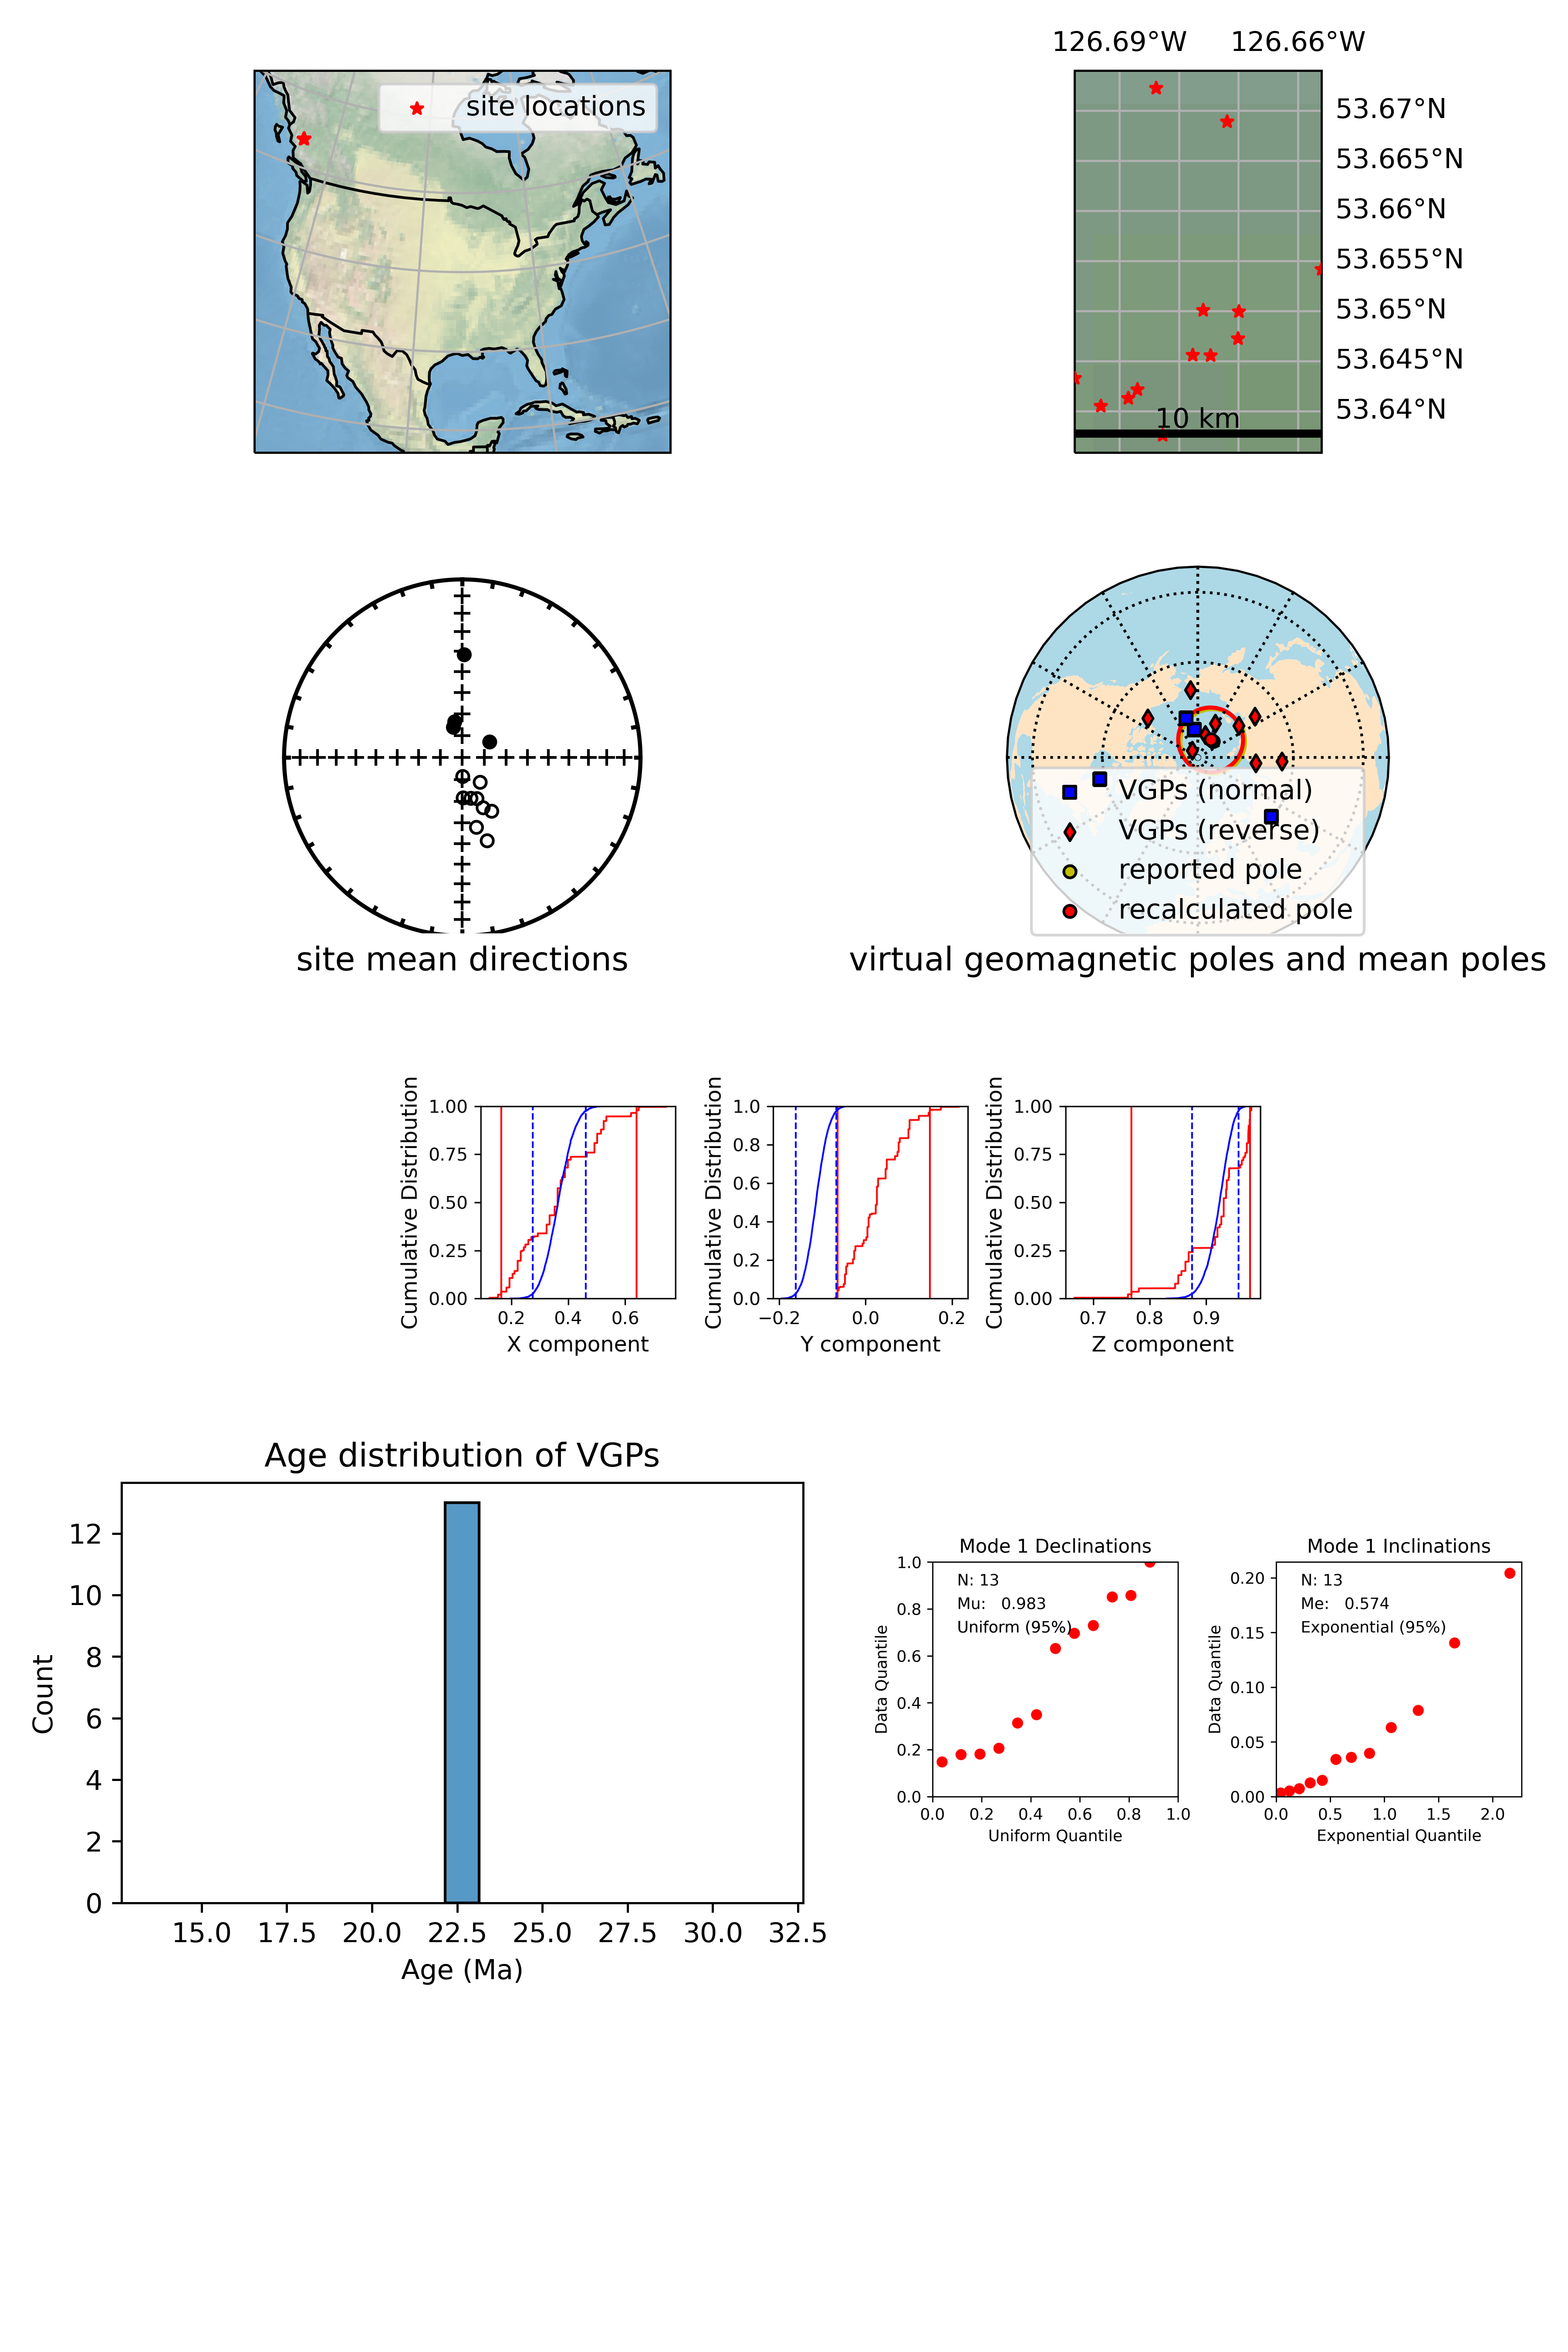
\includegraphics[width=5 in]{./19/1/pole_summary.png}
\caption{Summary of data from locality 19 (Dinan Bay lavas) pole 1 (Irving et al. (2000)).}
\end{figure}

\section{Valles Caldera volcanics}
\subsection{Pole 1}
\begin{tabular}{lllll}
\toprule
{} &   N &  Plat &   Plon &  A95 \\
\midrule
Reported mean pole                                 &  33 &  88.0 &  265.5 &  5.0 \\
Mean pole (calculated from VGPs)                   &  33 &  87.9 &  270.8 &  5.1 \\
Mean pole (calculated from transformed directions) &  33 &  87.9 &  270.6 &  5.1 \\
\bottomrule
\end{tabular}

\begin{tabular}{ll}
\toprule
{} &                                                          result \\
\midrule
Bootstrap reversal test  &                                                            Pass \\
Parametric reversal test &  Pass (angle 3.1º below 11.5º critical angle); C classification \\
Bayesian reversal test   &                                   Common mean: positive support \\
Fisher Q-Q test          &                             Consistent with Fisher distribution \\
\bottomrule
\end{tabular}

\begin{figure}[H]
\centering
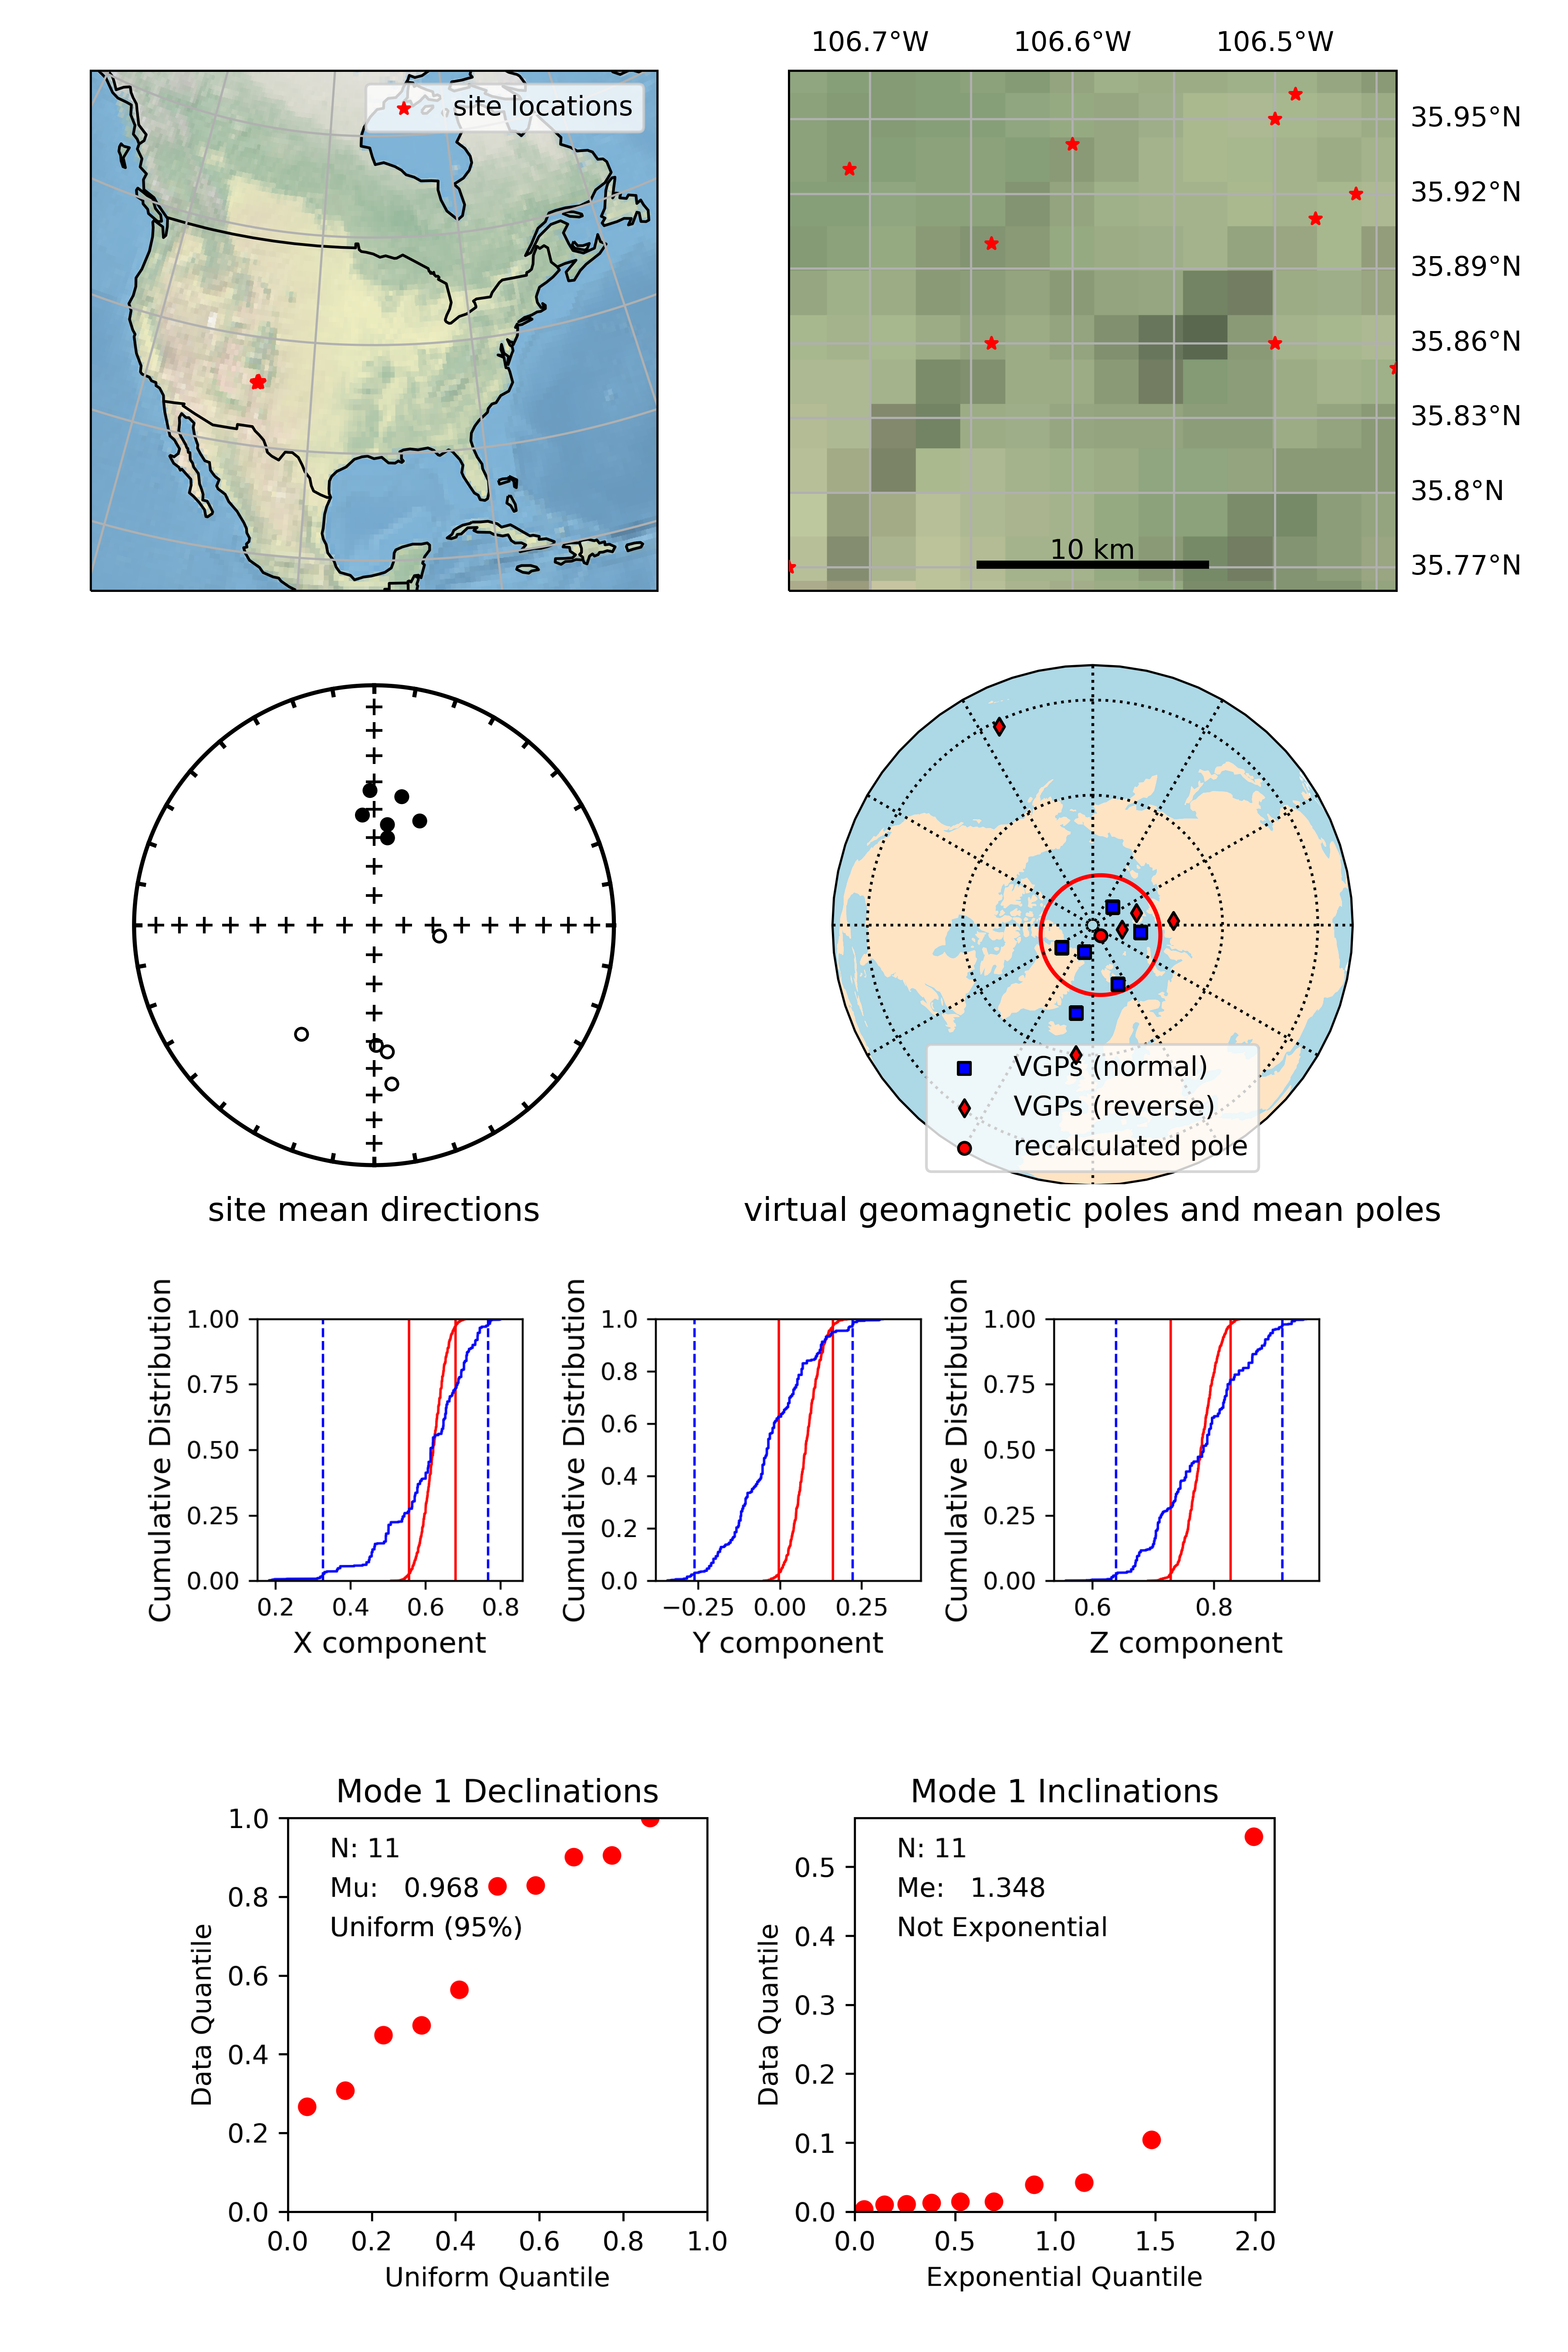
\includegraphics[width=5 in]{./20/1/pole_summary.png}
\caption{Summary of data from locality 20 (Valles Caldera volcanics) pole 1 (Doell et al. (1968)).}
\end{figure}

\section{Bitterroot Dome intrusions}
\subsection{Pole 1}
\begin{tabular}{lllll}
\toprule
{} &   N &  Plat &   Plon &  A95 \\
\midrule
Reported mean pole                                 &  33 &  88.0 &  265.5 &  5.0 \\
Mean pole (calculated from VGPs)                   &  33 &  87.9 &  270.8 &  5.1 \\
Mean pole (calculated from transformed directions) &  33 &  87.9 &  270.6 &  5.1 \\
\bottomrule
\end{tabular}

\begin{tabular}{ll}
\toprule
{} &                                                          result \\
\midrule
Bootstrap reversal test  &                                                            Pass \\
Parametric reversal test &  Pass (angle 3.1º below 11.5º critical angle); C classification \\
Bayesian reversal test   &                                   Common mean: positive support \\
Fisher Q-Q test          &                             Consistent with Fisher distribution \\
\bottomrule
\end{tabular}

\begin{figure}[H]
\centering
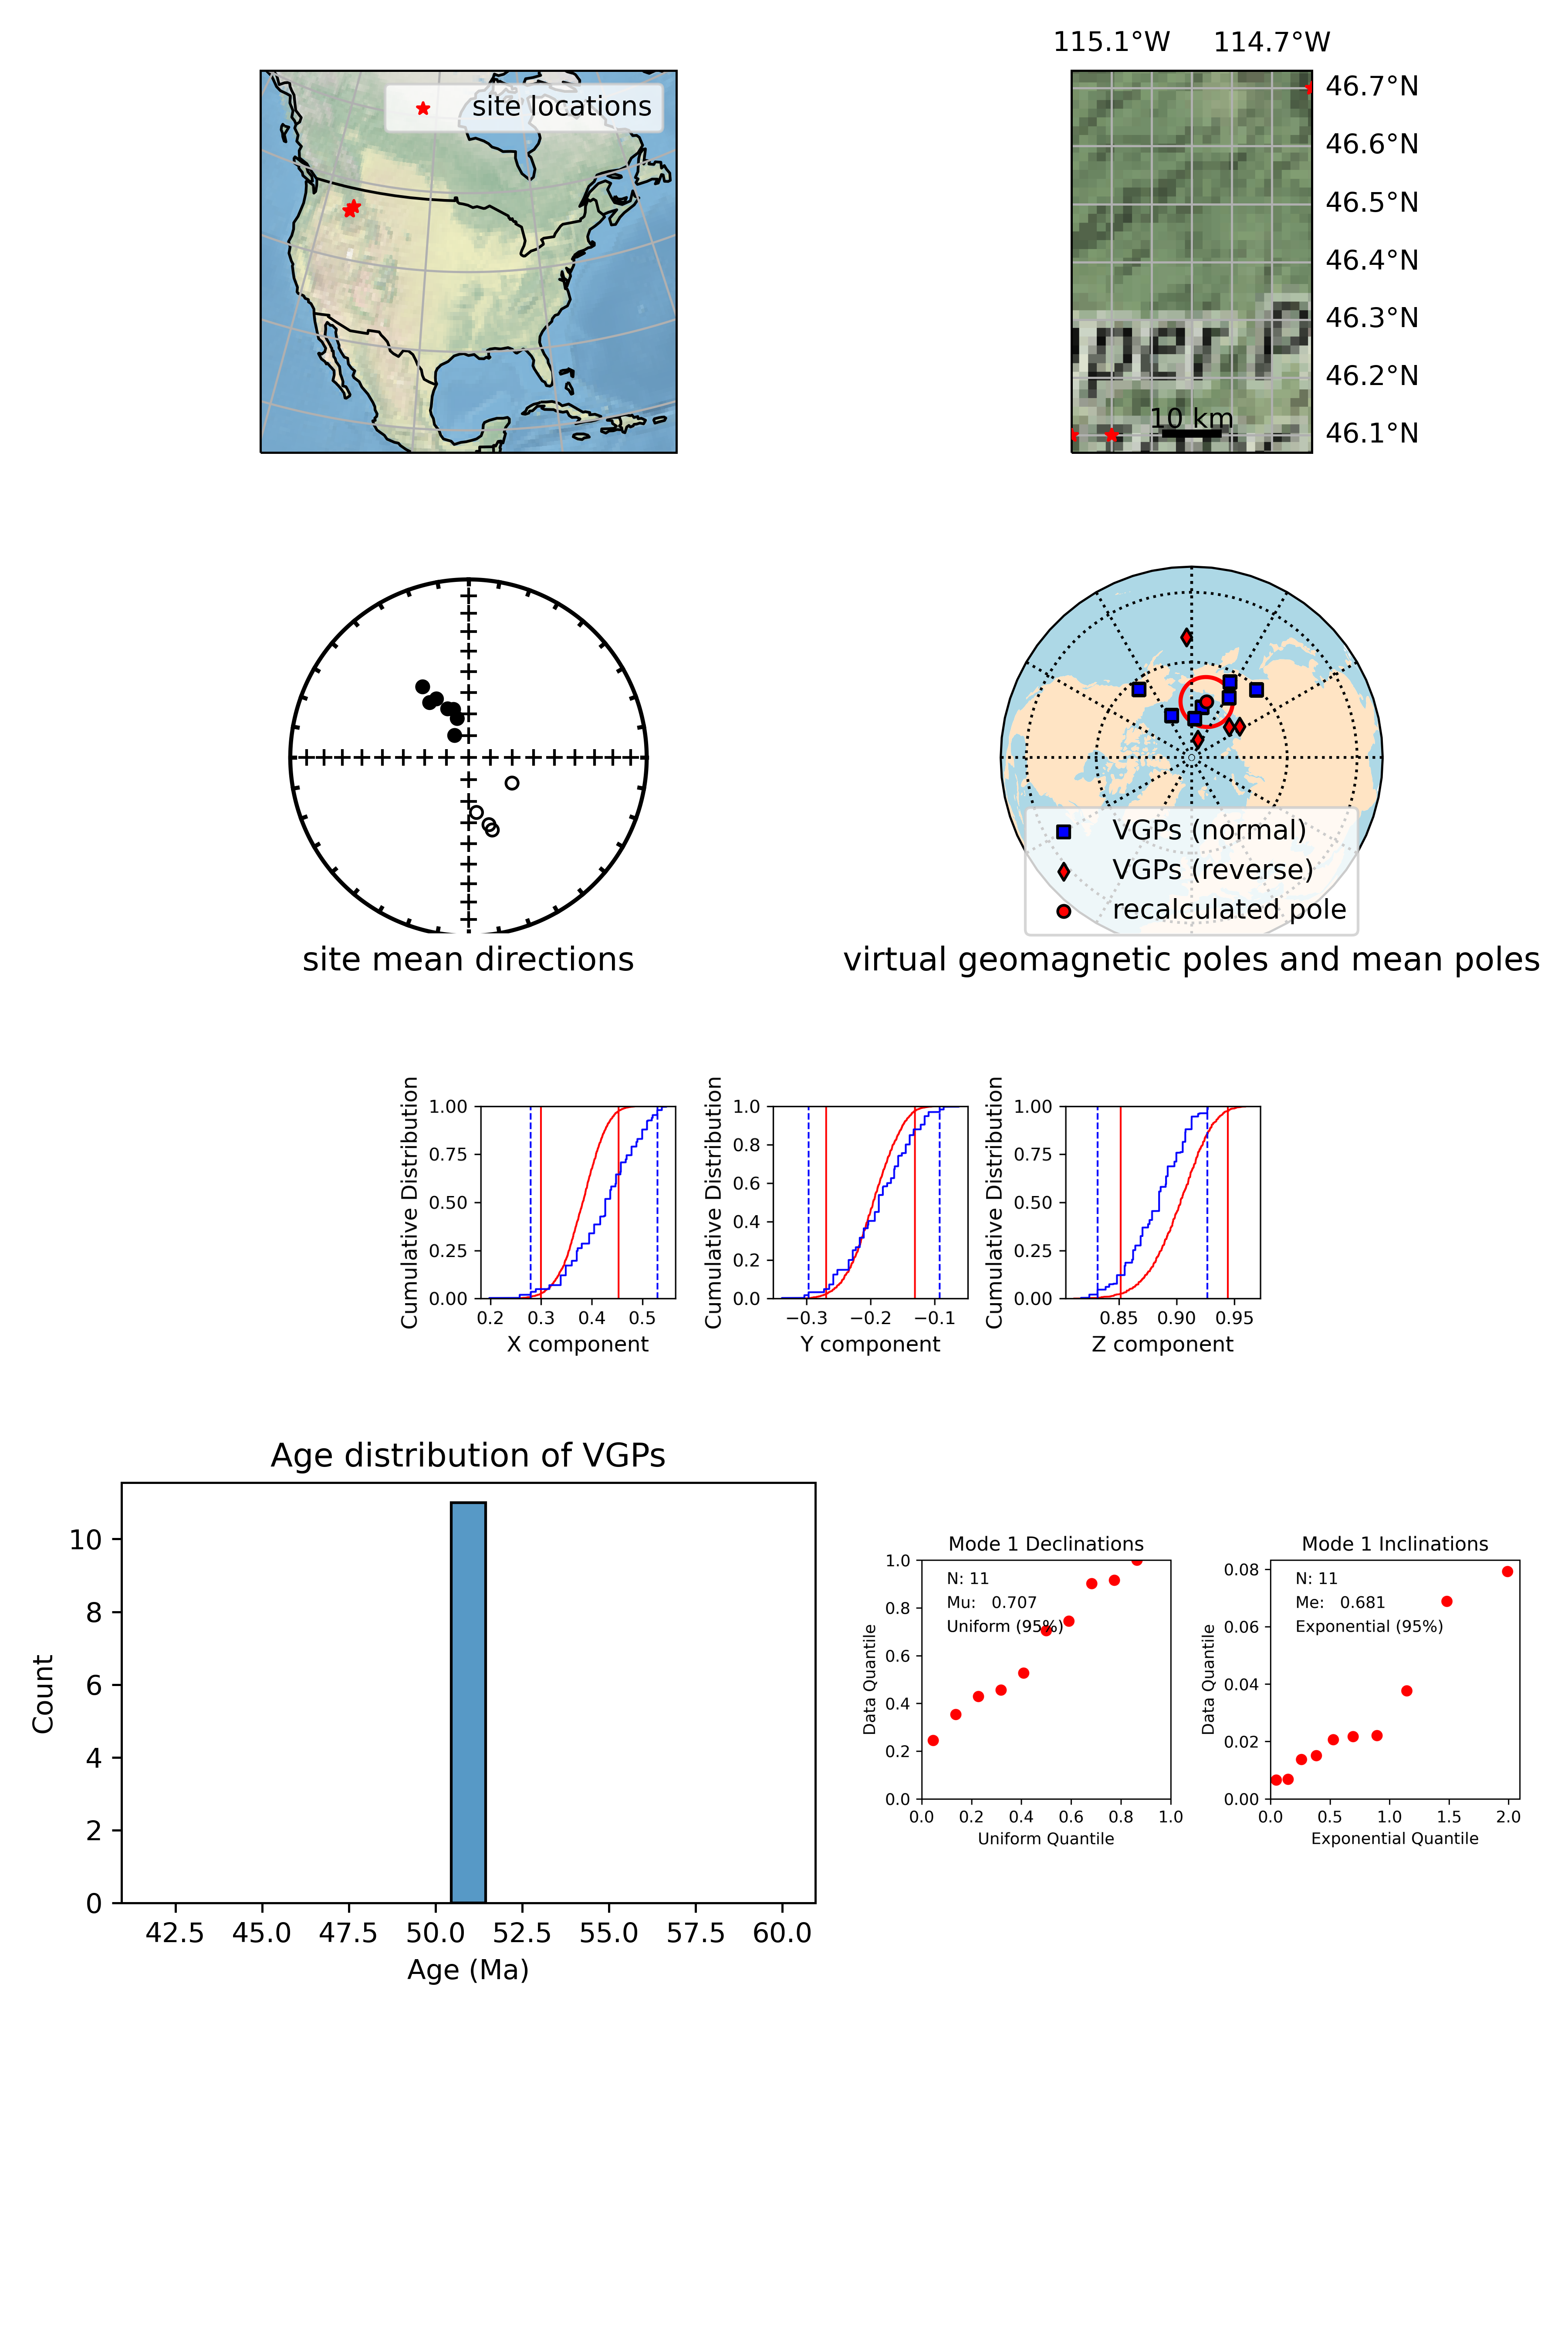
\includegraphics[width=5 in]{./21/1/pole_summary.png}
\caption{Summary of data from locality 21 (Bitterroot Dome intrusions) pole 1 (Doughty and Sheriff (1992)).}
\end{figure}

\section{Stoddard Mountain laccolith}
\subsection{Pole 1}
\begin{tabular}{lllll}
\toprule
{} &   N &  Plat &   Plon &  A95 \\
\midrule
Reported mean pole                                 &  33 &  88.0 &  265.5 &  5.0 \\
Mean pole (calculated from VGPs)                   &  33 &  87.9 &  270.8 &  5.1 \\
Mean pole (calculated from transformed directions) &  33 &  87.9 &  270.6 &  5.1 \\
\bottomrule
\end{tabular}

\begin{tabular}{ll}
\toprule
{} &                                                          result \\
\midrule
Bootstrap reversal test  &                                                            Pass \\
Parametric reversal test &  Pass (angle 3.1º below 11.5º critical angle); C classification \\
Bayesian reversal test   &                                   Common mean: positive support \\
Fisher Q-Q test          &                             Consistent with Fisher distribution \\
\bottomrule
\end{tabular}

\begin{figure}[H]
\centering
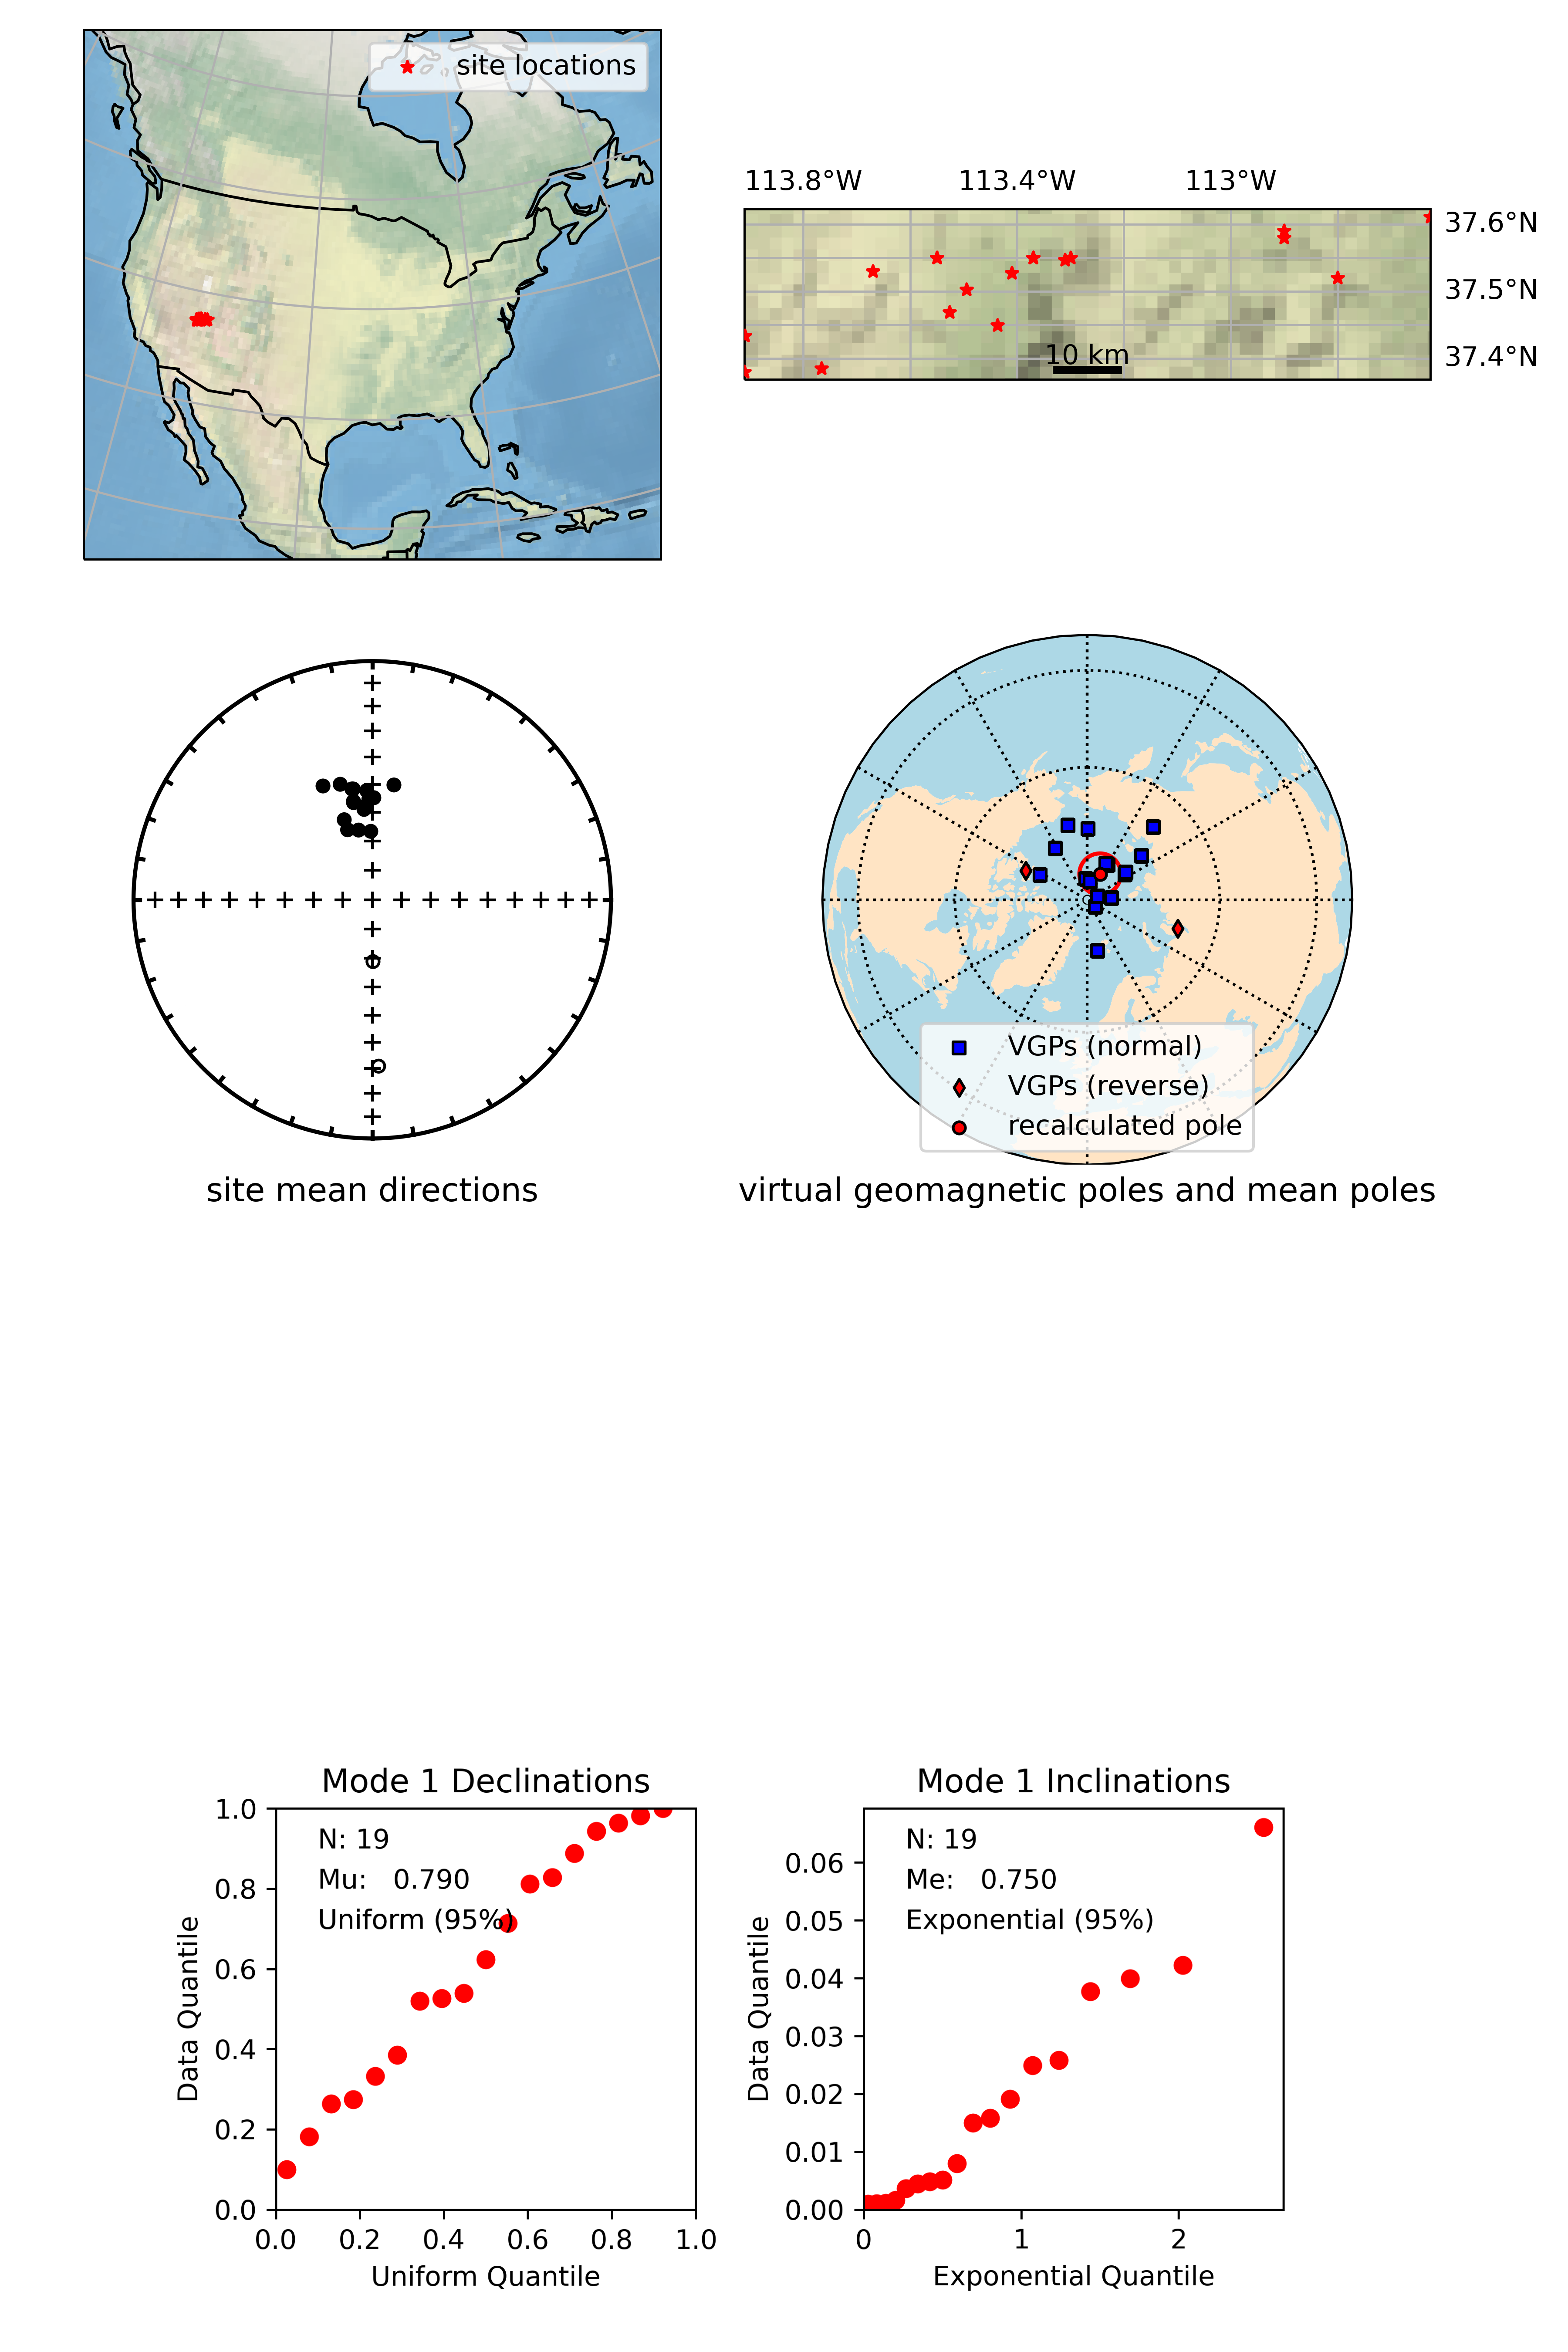
\includegraphics[width=5 in]{./22/1/pole_summary.png}
\caption{Summary of data from locality 22 (Stoddard Mountain laccolith) pole 1 (Petronis et al. (2004)).}
\end{figure}

\section{Michoacan Guanajuato volcanic field}
\subsection{Pole 1}
\begin{tabular}{lllll}
\toprule
{} &   N &  Plat &   Plon &  A95 \\
\midrule
Reported mean pole                                 &  33 &  88.0 &  265.5 &  5.0 \\
Mean pole (calculated from VGPs)                   &  33 &  87.9 &  270.8 &  5.1 \\
Mean pole (calculated from transformed directions) &  33 &  87.9 &  270.6 &  5.1 \\
\bottomrule
\end{tabular}

\begin{tabular}{ll}
\toprule
{} &                                                          result \\
\midrule
Bootstrap reversal test  &                                                            Pass \\
Parametric reversal test &  Pass (angle 3.1º below 11.5º critical angle); C classification \\
Bayesian reversal test   &                                   Common mean: positive support \\
Fisher Q-Q test          &                             Consistent with Fisher distribution \\
\bottomrule
\end{tabular}

\begin{figure}[H]
\centering
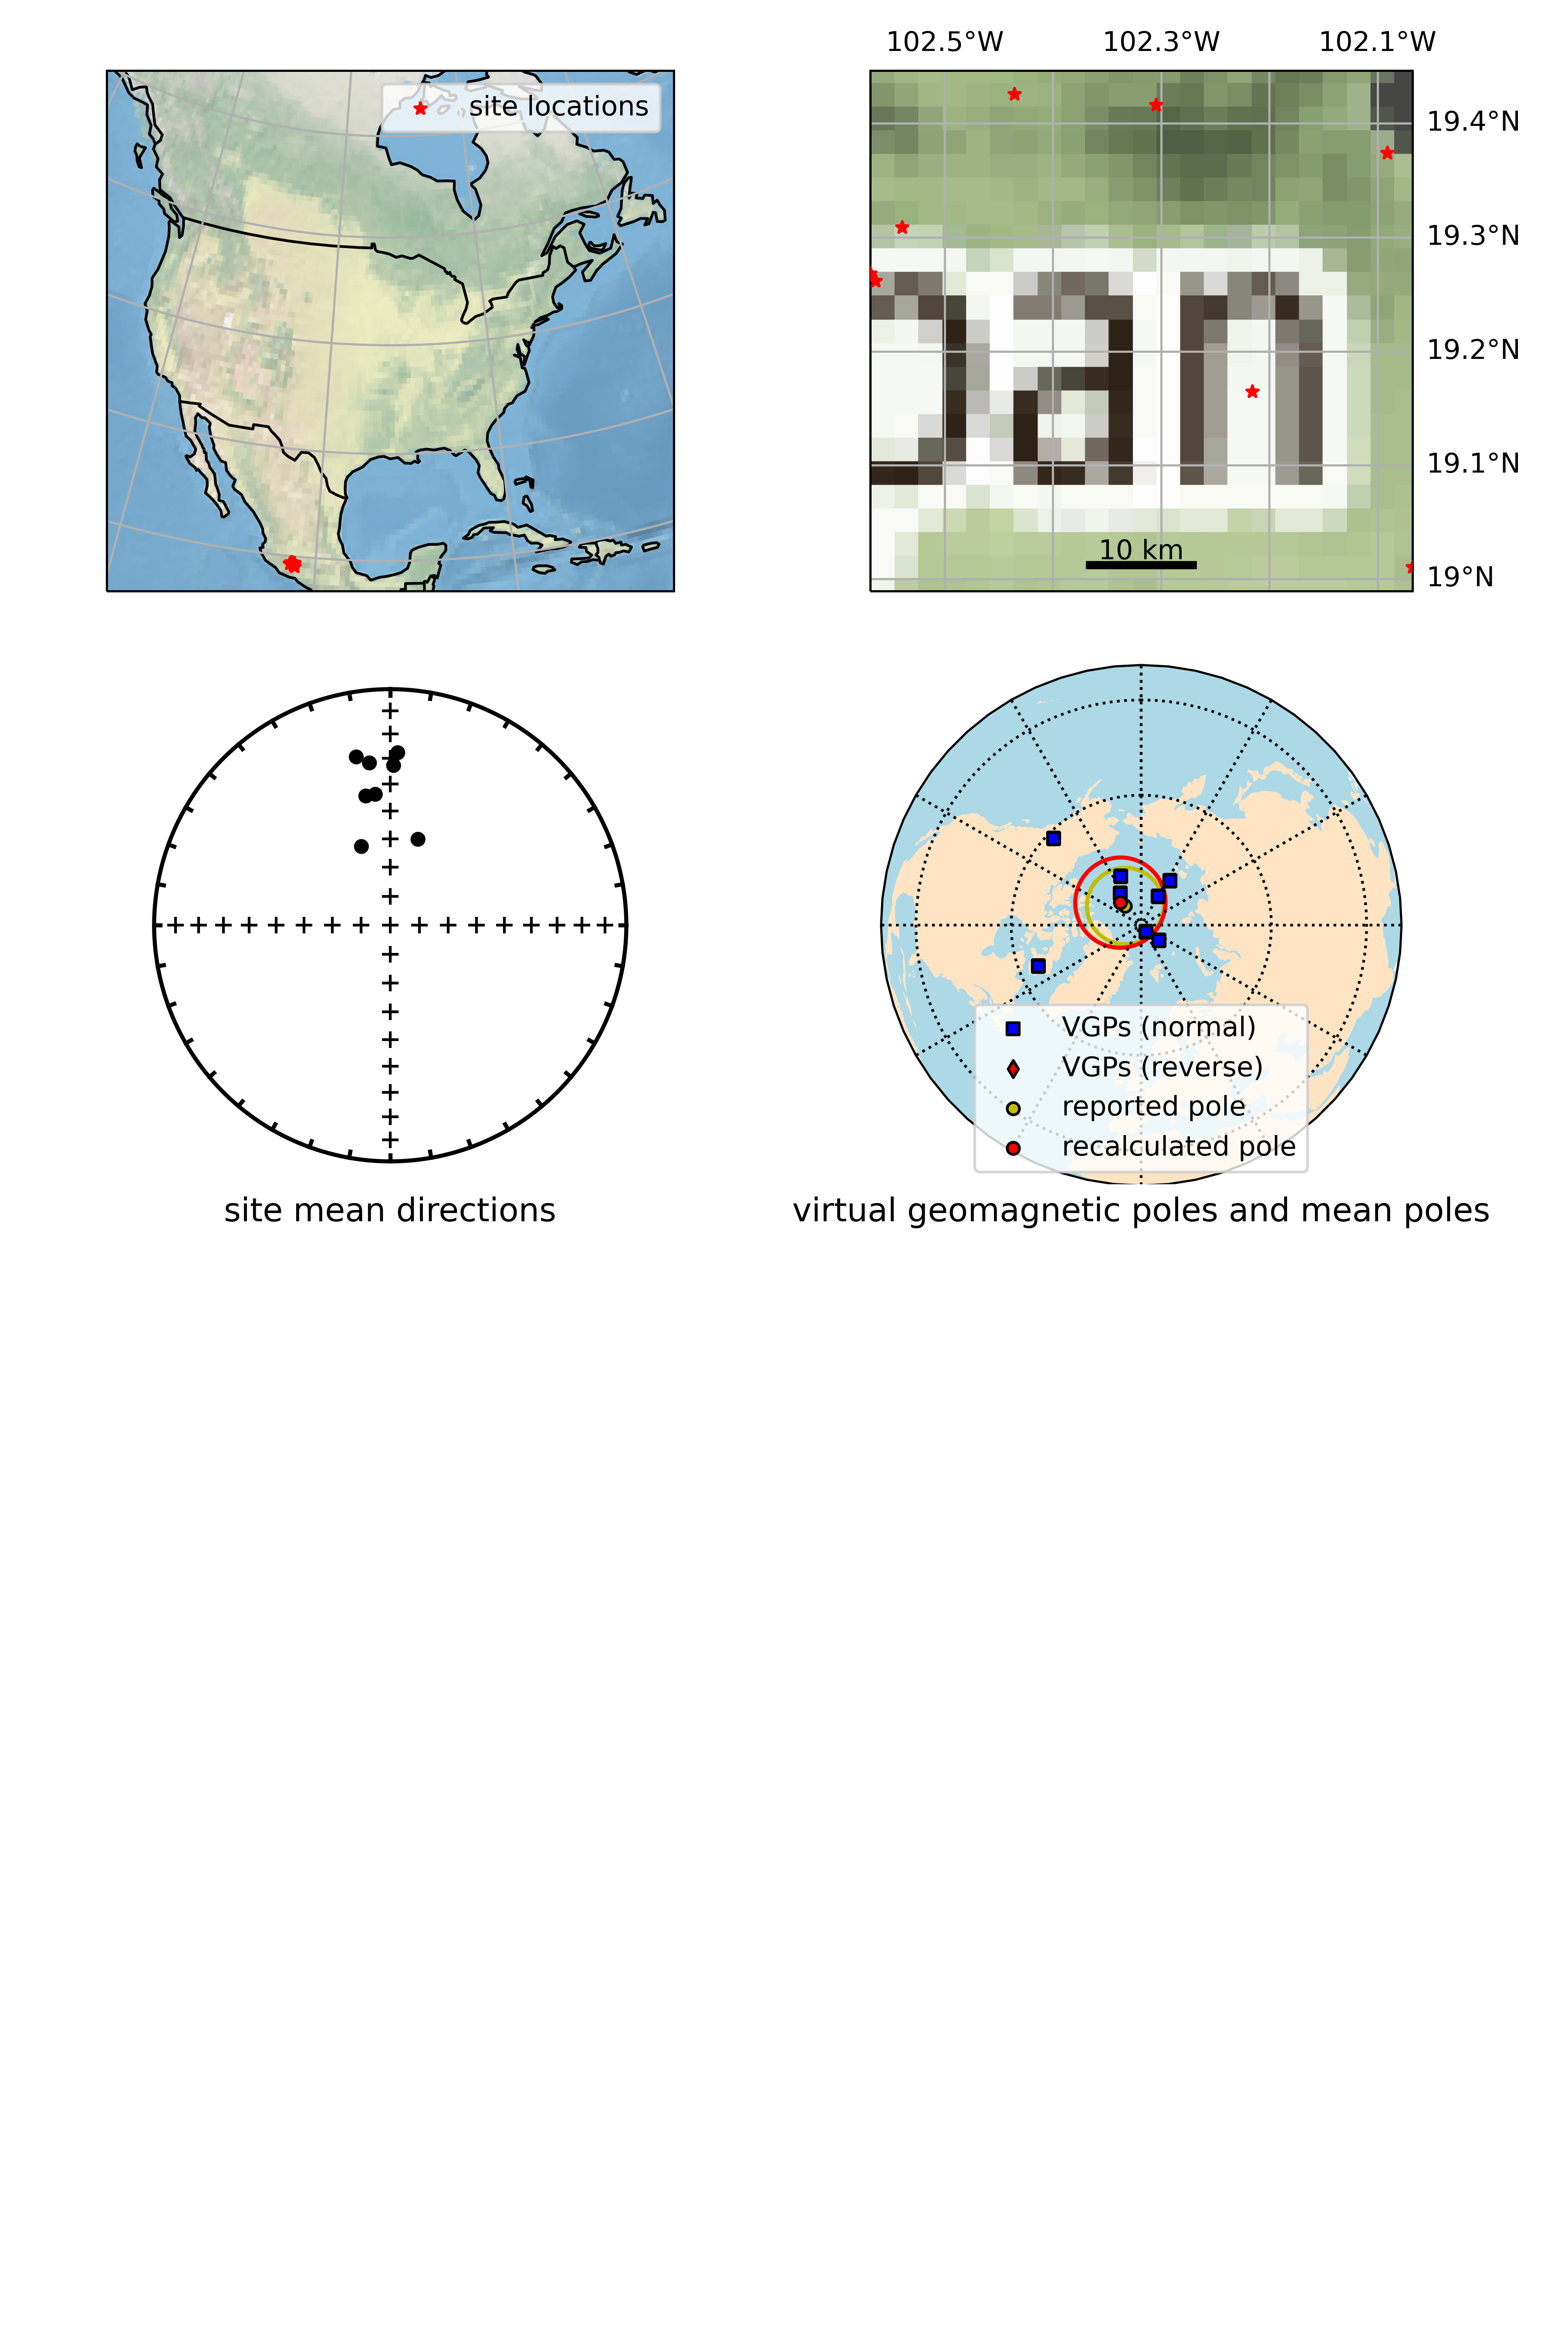
\includegraphics[width=5 in]{./23/1/pole_summary.png}
\caption{Summary of data from locality 23 (Michoacan Guanajuato volcanic field) pole 1 (Maciel Peña et al. (2009)).}
\end{figure}

\section{Clear Lake volcanic field}
\subsection{Pole 1}
\begin{tabular}{lllll}
\toprule
{} &   N &  Plat &   Plon &  A95 \\
\midrule
Reported mean pole                                 &  33 &  88.0 &  265.5 &  5.0 \\
Mean pole (calculated from VGPs)                   &  33 &  87.9 &  270.8 &  5.1 \\
Mean pole (calculated from transformed directions) &  33 &  87.9 &  270.6 &  5.1 \\
\bottomrule
\end{tabular}

\begin{tabular}{ll}
\toprule
{} &                                                          result \\
\midrule
Bootstrap reversal test  &                                                            Pass \\
Parametric reversal test &  Pass (angle 3.1º below 11.5º critical angle); C classification \\
Bayesian reversal test   &                                   Common mean: positive support \\
Fisher Q-Q test          &                             Consistent with Fisher distribution \\
\bottomrule
\end{tabular}

\begin{figure}[H]
\centering
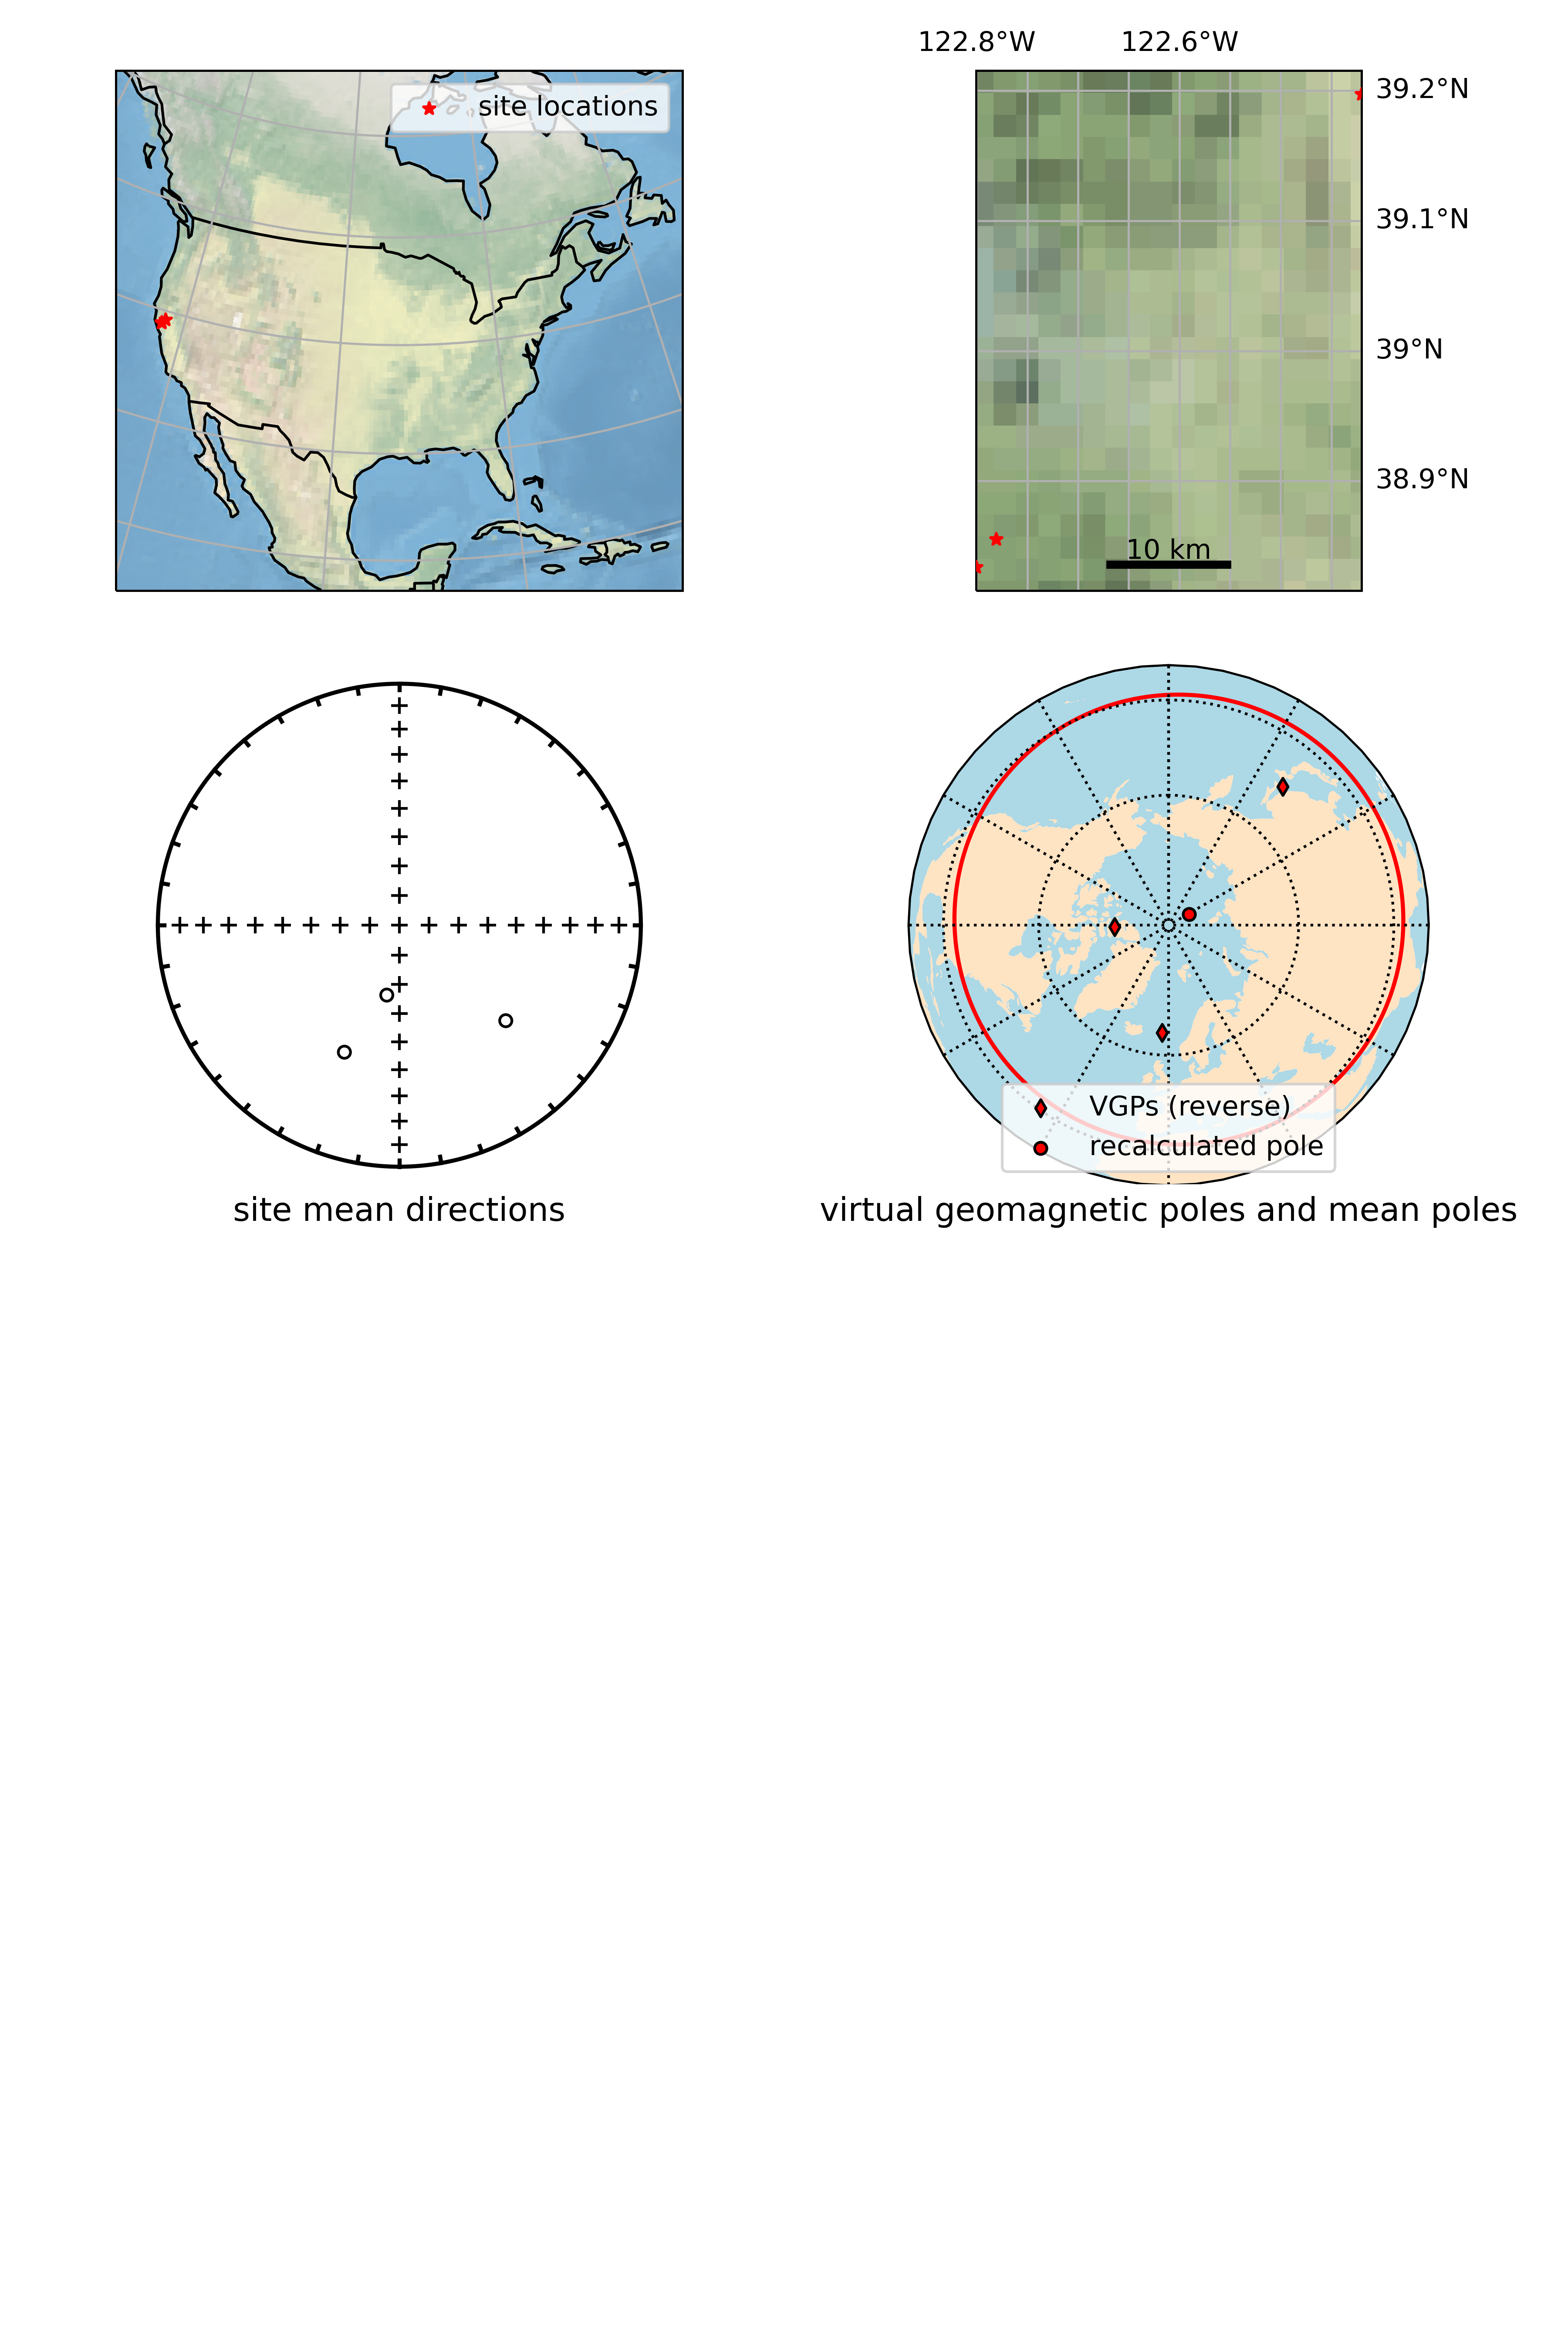
\includegraphics[width=5 in]{./24/1/pole_summary.png}
\caption{Summary of data from locality 24 (Clear Lake volcanic field) pole 1 (Mankinen et al. (1978); Mankinen et al. (1981)).}
\end{figure}

\section{San Luis Hills volcanics}
\subsection{Pole 1}
\begin{tabular}{lllll}
\toprule
{} &   N &  Plat &   Plon &  A95 \\
\midrule
Reported mean pole                                 &  33 &  88.0 &  265.5 &  5.0 \\
Mean pole (calculated from VGPs)                   &  33 &  87.9 &  270.8 &  5.1 \\
Mean pole (calculated from transformed directions) &  33 &  87.9 &  270.6 &  5.1 \\
\bottomrule
\end{tabular}

\begin{tabular}{ll}
\toprule
{} &                                                          result \\
\midrule
Bootstrap reversal test  &                                                            Pass \\
Parametric reversal test &  Pass (angle 3.1º below 11.5º critical angle); C classification \\
Bayesian reversal test   &                                   Common mean: positive support \\
Fisher Q-Q test          &                             Consistent with Fisher distribution \\
\bottomrule
\end{tabular}

\begin{figure}[H]
\centering
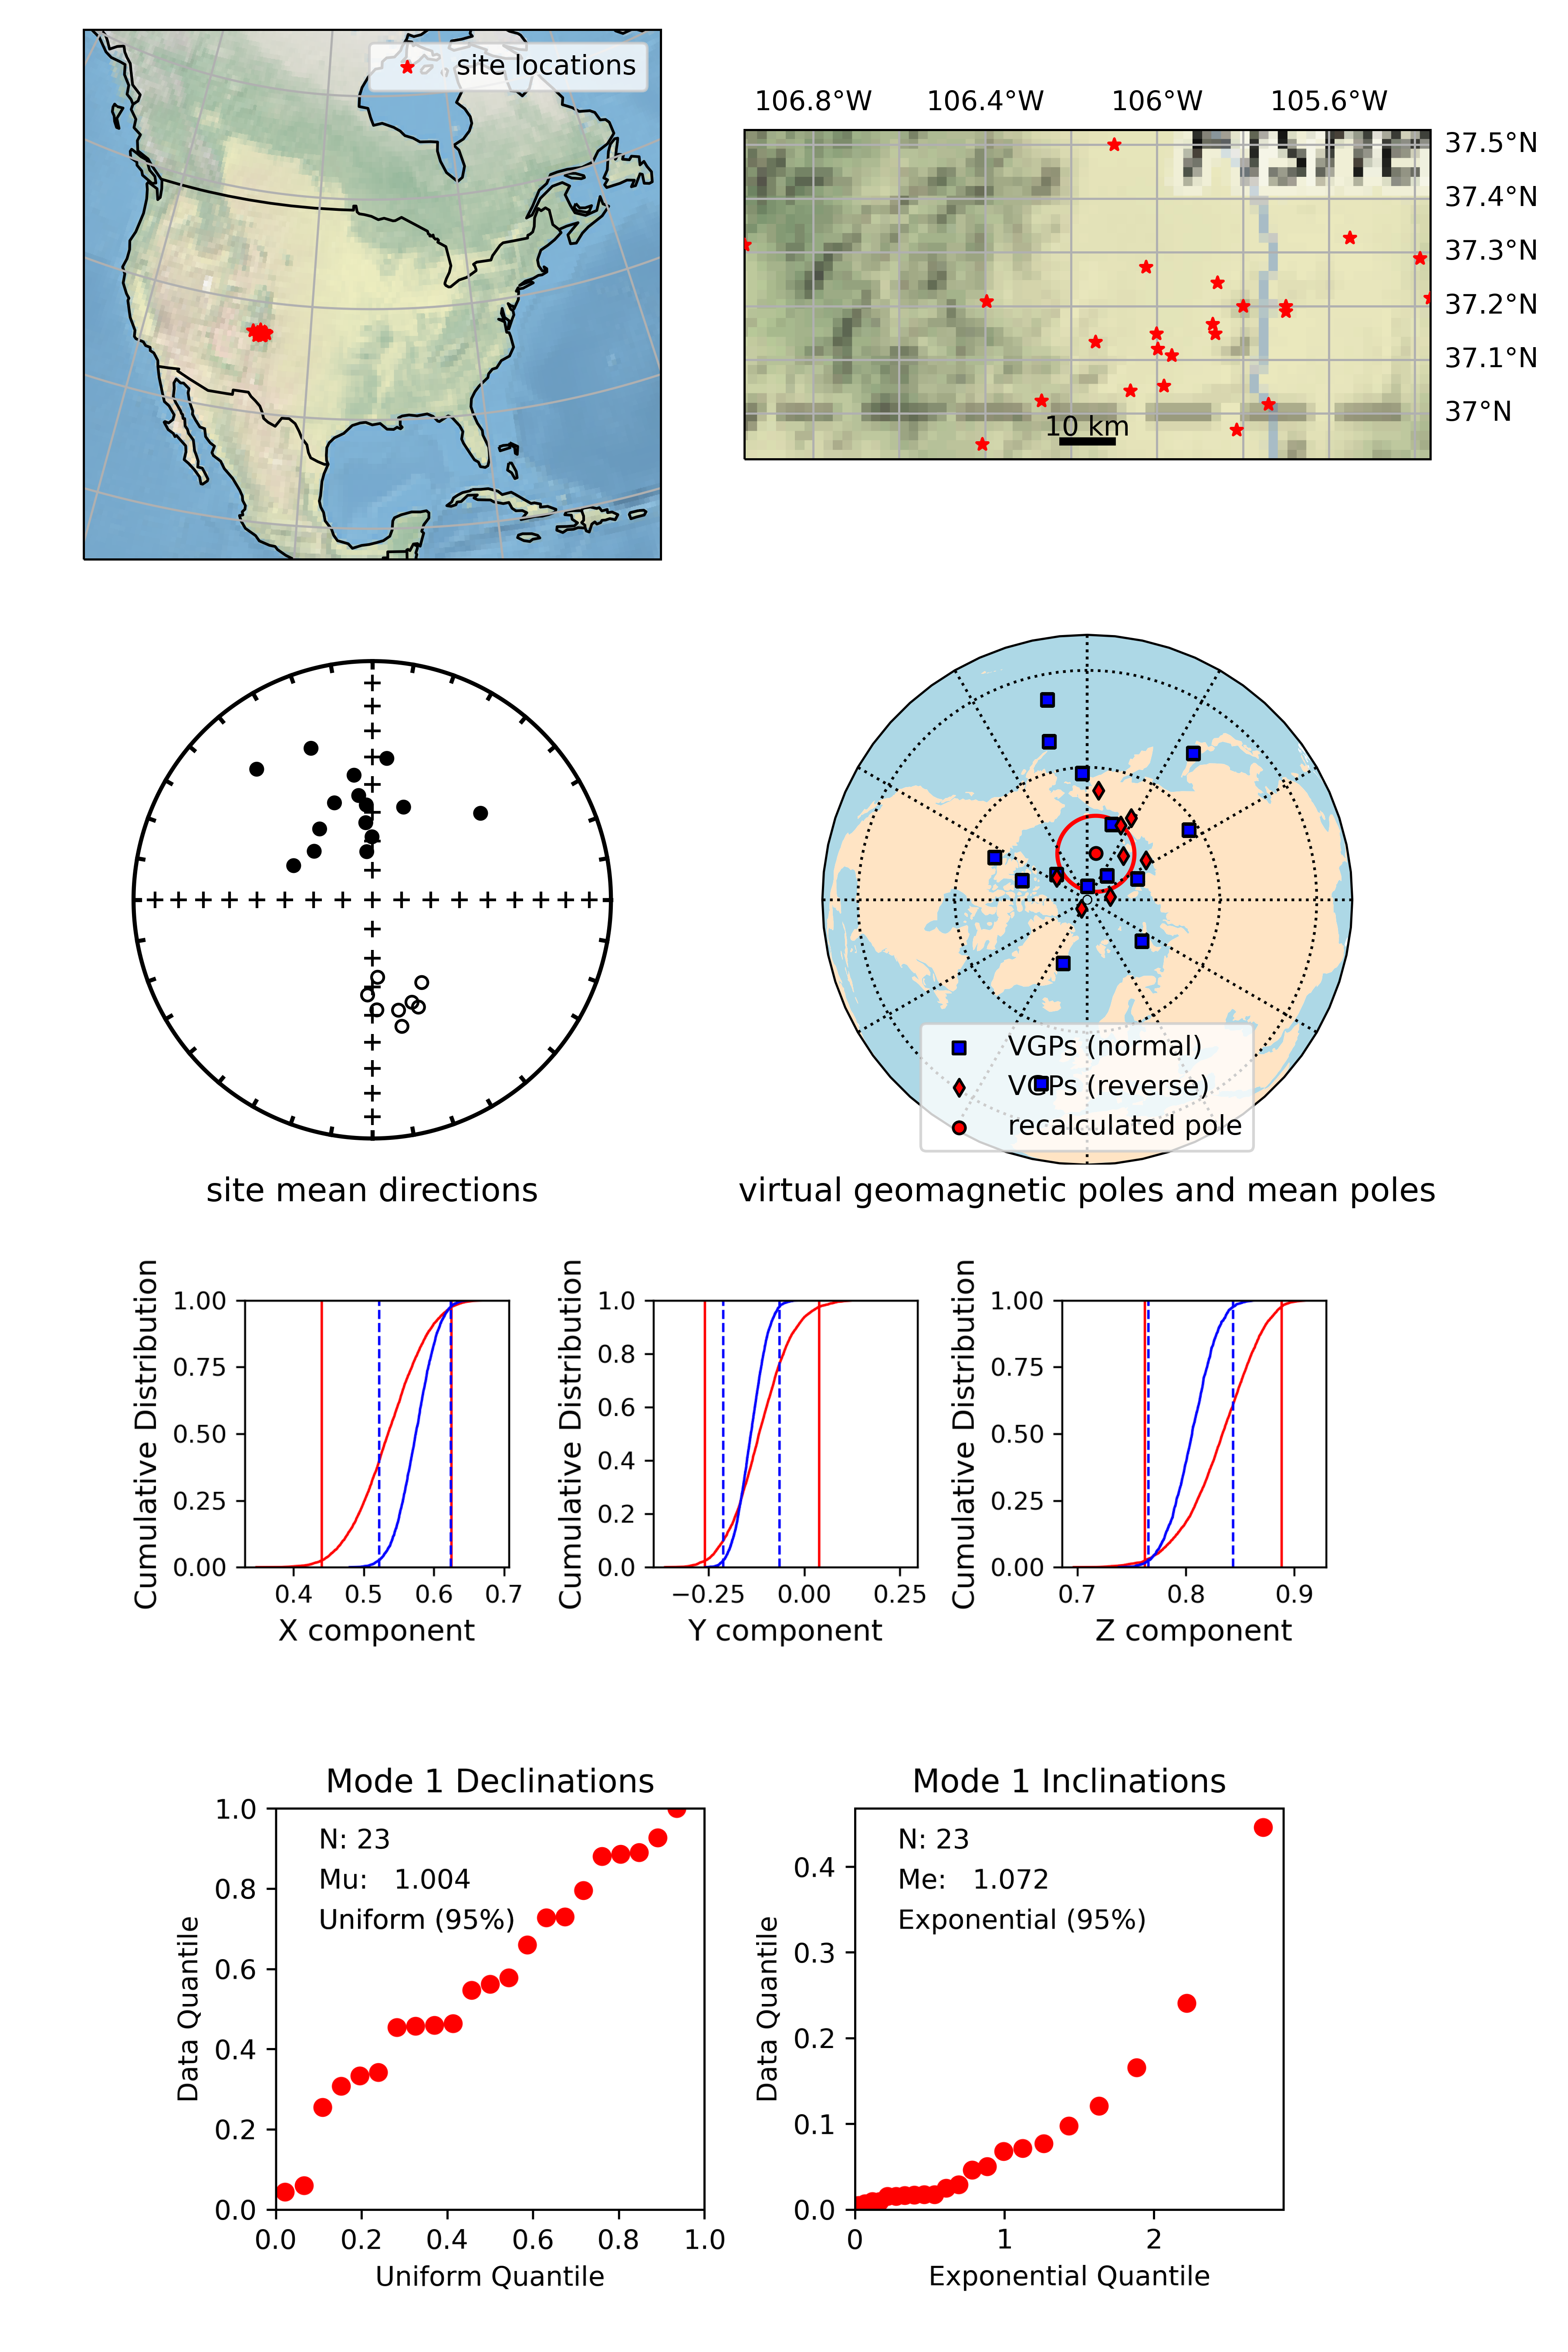
\includegraphics[width=5 in]{./25/1/pole_summary.png}
\caption{Summary of data from locality 25 (San Luis Hills volcanics) pole 1 (Brown and Golombek (1997)).}
\end{figure}

\section{Beaver River intrusions}
\subsection{Pole 1}
\begin{tabular}{lllll}
\toprule
{} &   N &  Plat &   Plon &  A95 \\
\midrule
Reported mean pole                                 &  33 &  88.0 &  265.5 &  5.0 \\
Mean pole (calculated from VGPs)                   &  33 &  87.9 &  270.8 &  5.1 \\
Mean pole (calculated from transformed directions) &  33 &  87.9 &  270.6 &  5.1 \\
\bottomrule
\end{tabular}

\begin{tabular}{ll}
\toprule
{} &                                                          result \\
\midrule
Bootstrap reversal test  &                                                            Pass \\
Parametric reversal test &  Pass (angle 3.1º below 11.5º critical angle); C classification \\
Bayesian reversal test   &                                   Common mean: positive support \\
Fisher Q-Q test          &                             Consistent with Fisher distribution \\
\bottomrule
\end{tabular}

\begin{figure}[H]
\centering
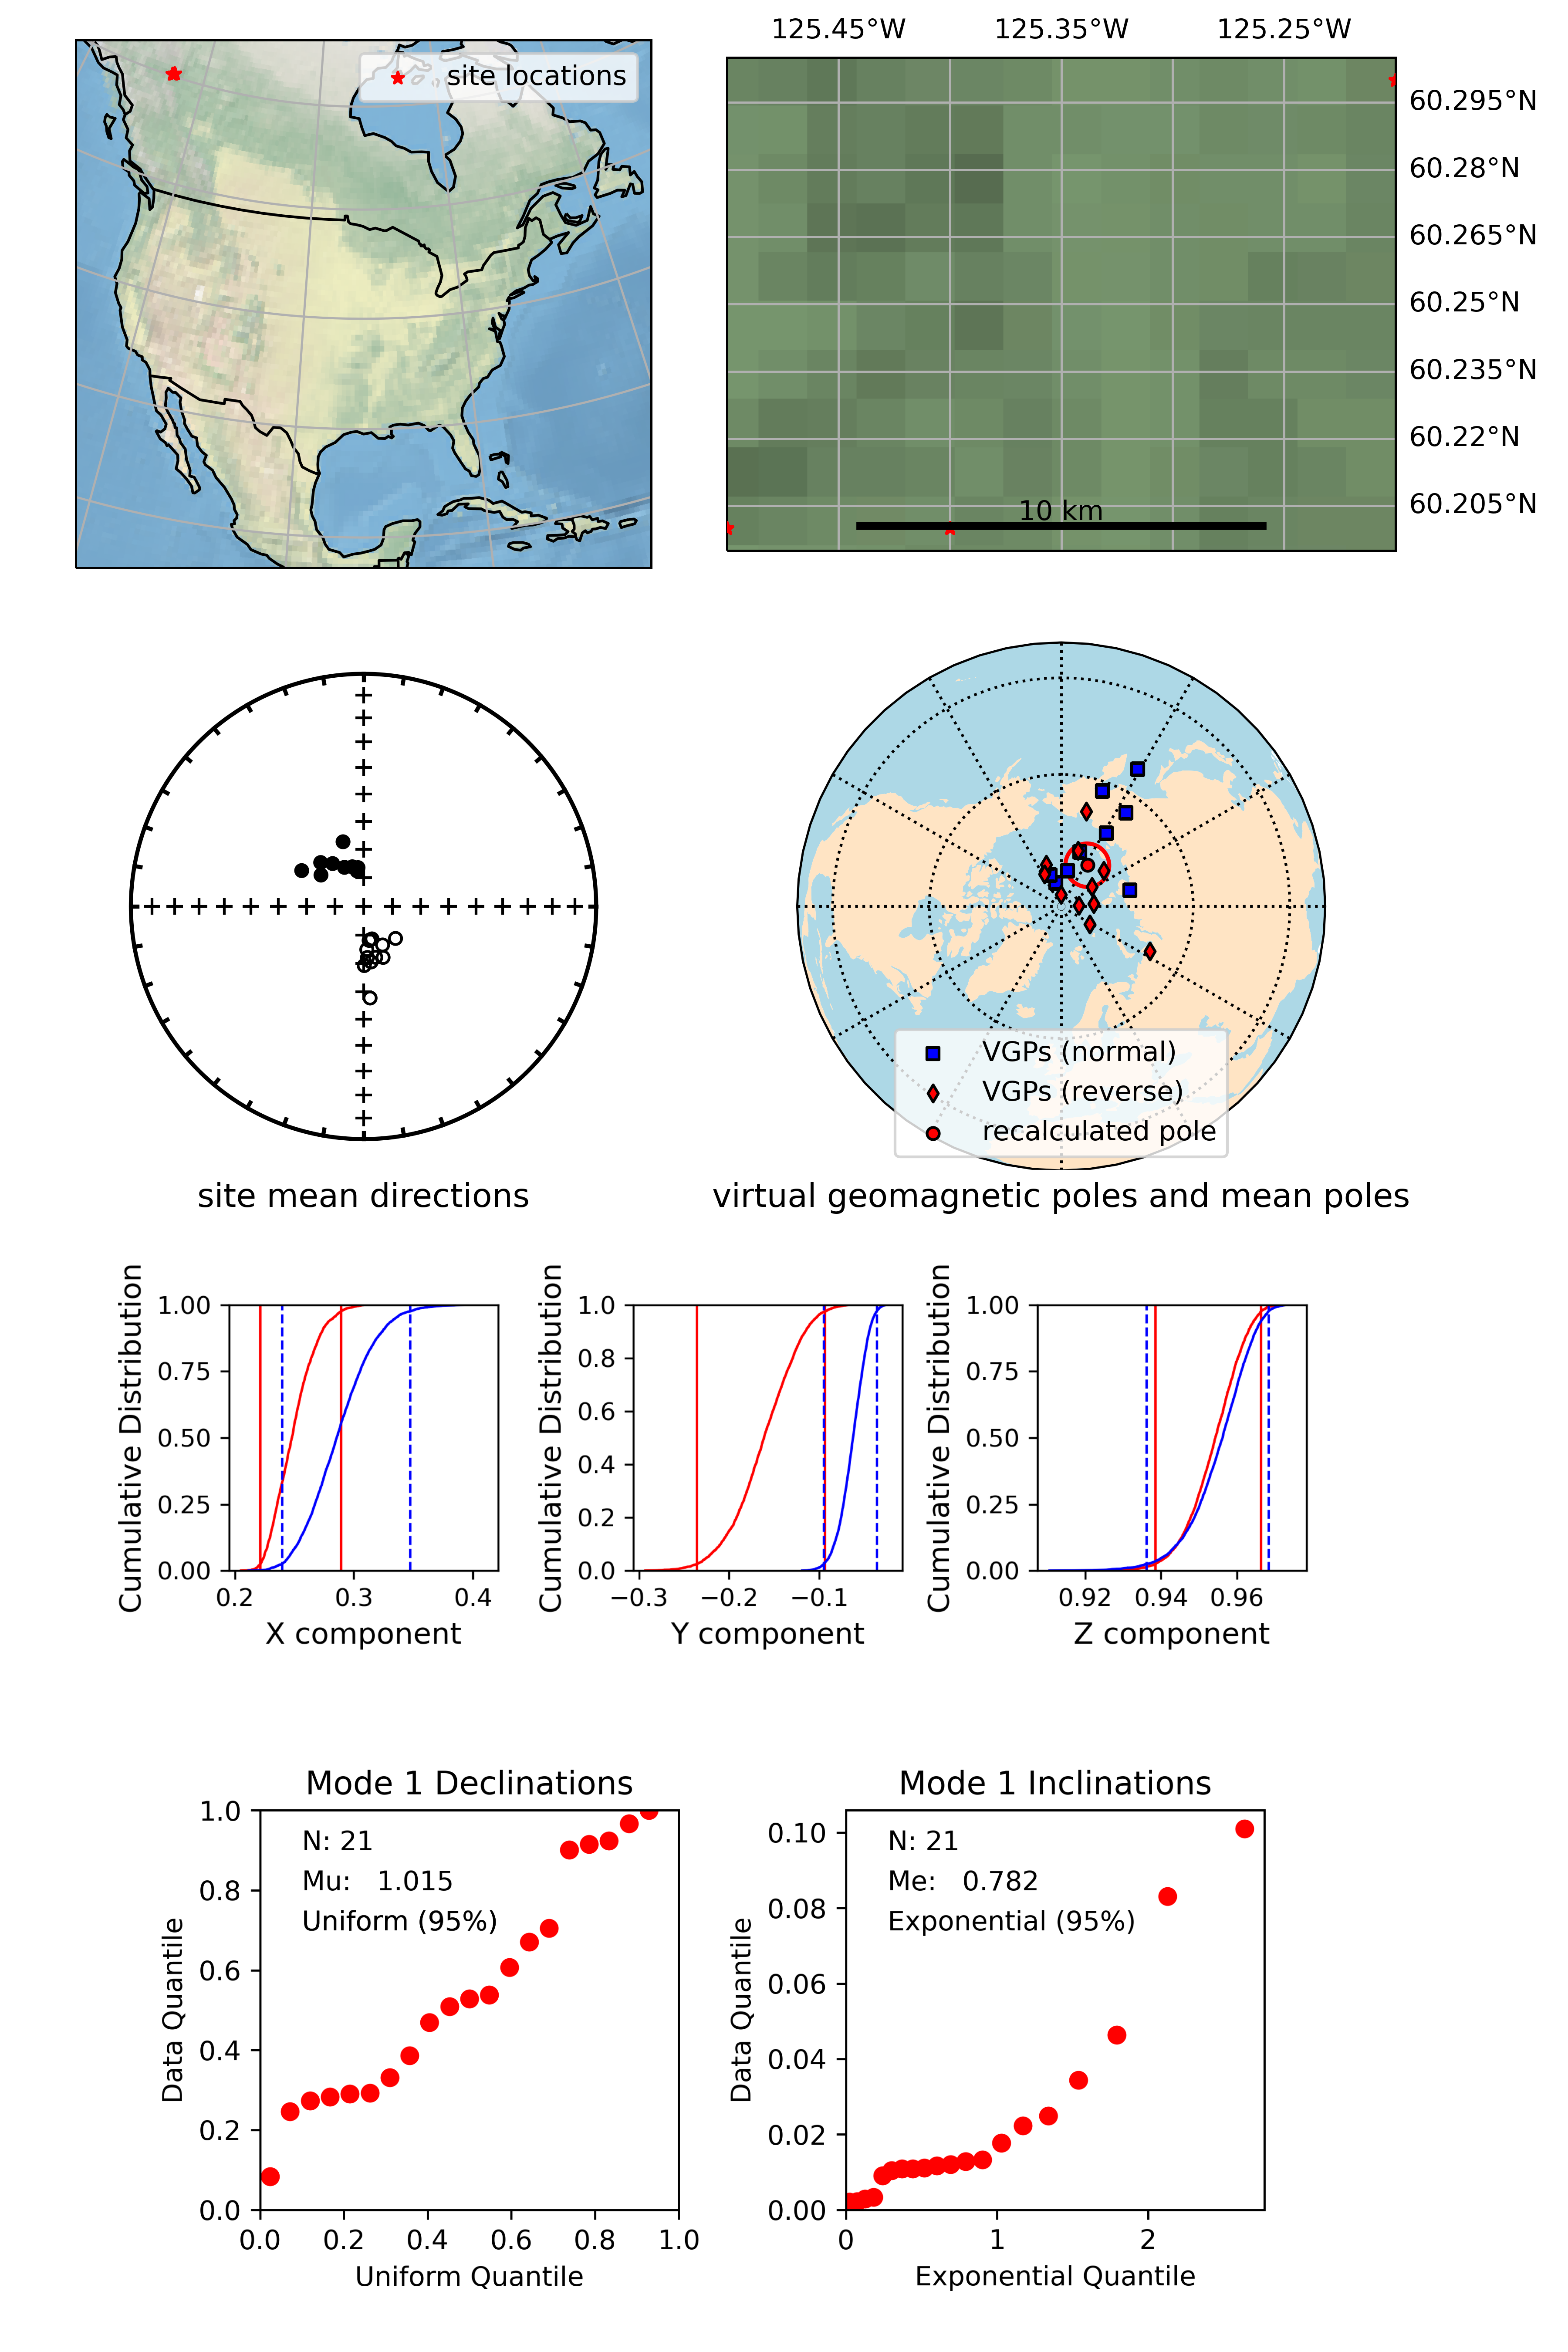
\includegraphics[width=5 in]{./26/1/pole_summary.png}
\caption{Summary of data from locality 26 (Beaver River intrusions) pole 1 (Symons et al. (2003)).}
\end{figure}

\section{Mariscal Mtn intrusions}
\subsection{Pole 1}
\begin{tabular}{lllll}
\toprule
{} &   N &  Plat &   Plon &  A95 \\
\midrule
Reported mean pole                                 &  33 &  88.0 &  265.5 &  5.0 \\
Mean pole (calculated from VGPs)                   &  33 &  87.9 &  270.8 &  5.1 \\
Mean pole (calculated from transformed directions) &  33 &  87.9 &  270.6 &  5.1 \\
\bottomrule
\end{tabular}

\begin{tabular}{ll}
\toprule
{} &                                                          result \\
\midrule
Bootstrap reversal test  &                                                            Pass \\
Parametric reversal test &  Pass (angle 3.1º below 11.5º critical angle); C classification \\
Bayesian reversal test   &                                   Common mean: positive support \\
Fisher Q-Q test          &                             Consistent with Fisher distribution \\
\bottomrule
\end{tabular}

\begin{figure}[H]
\centering
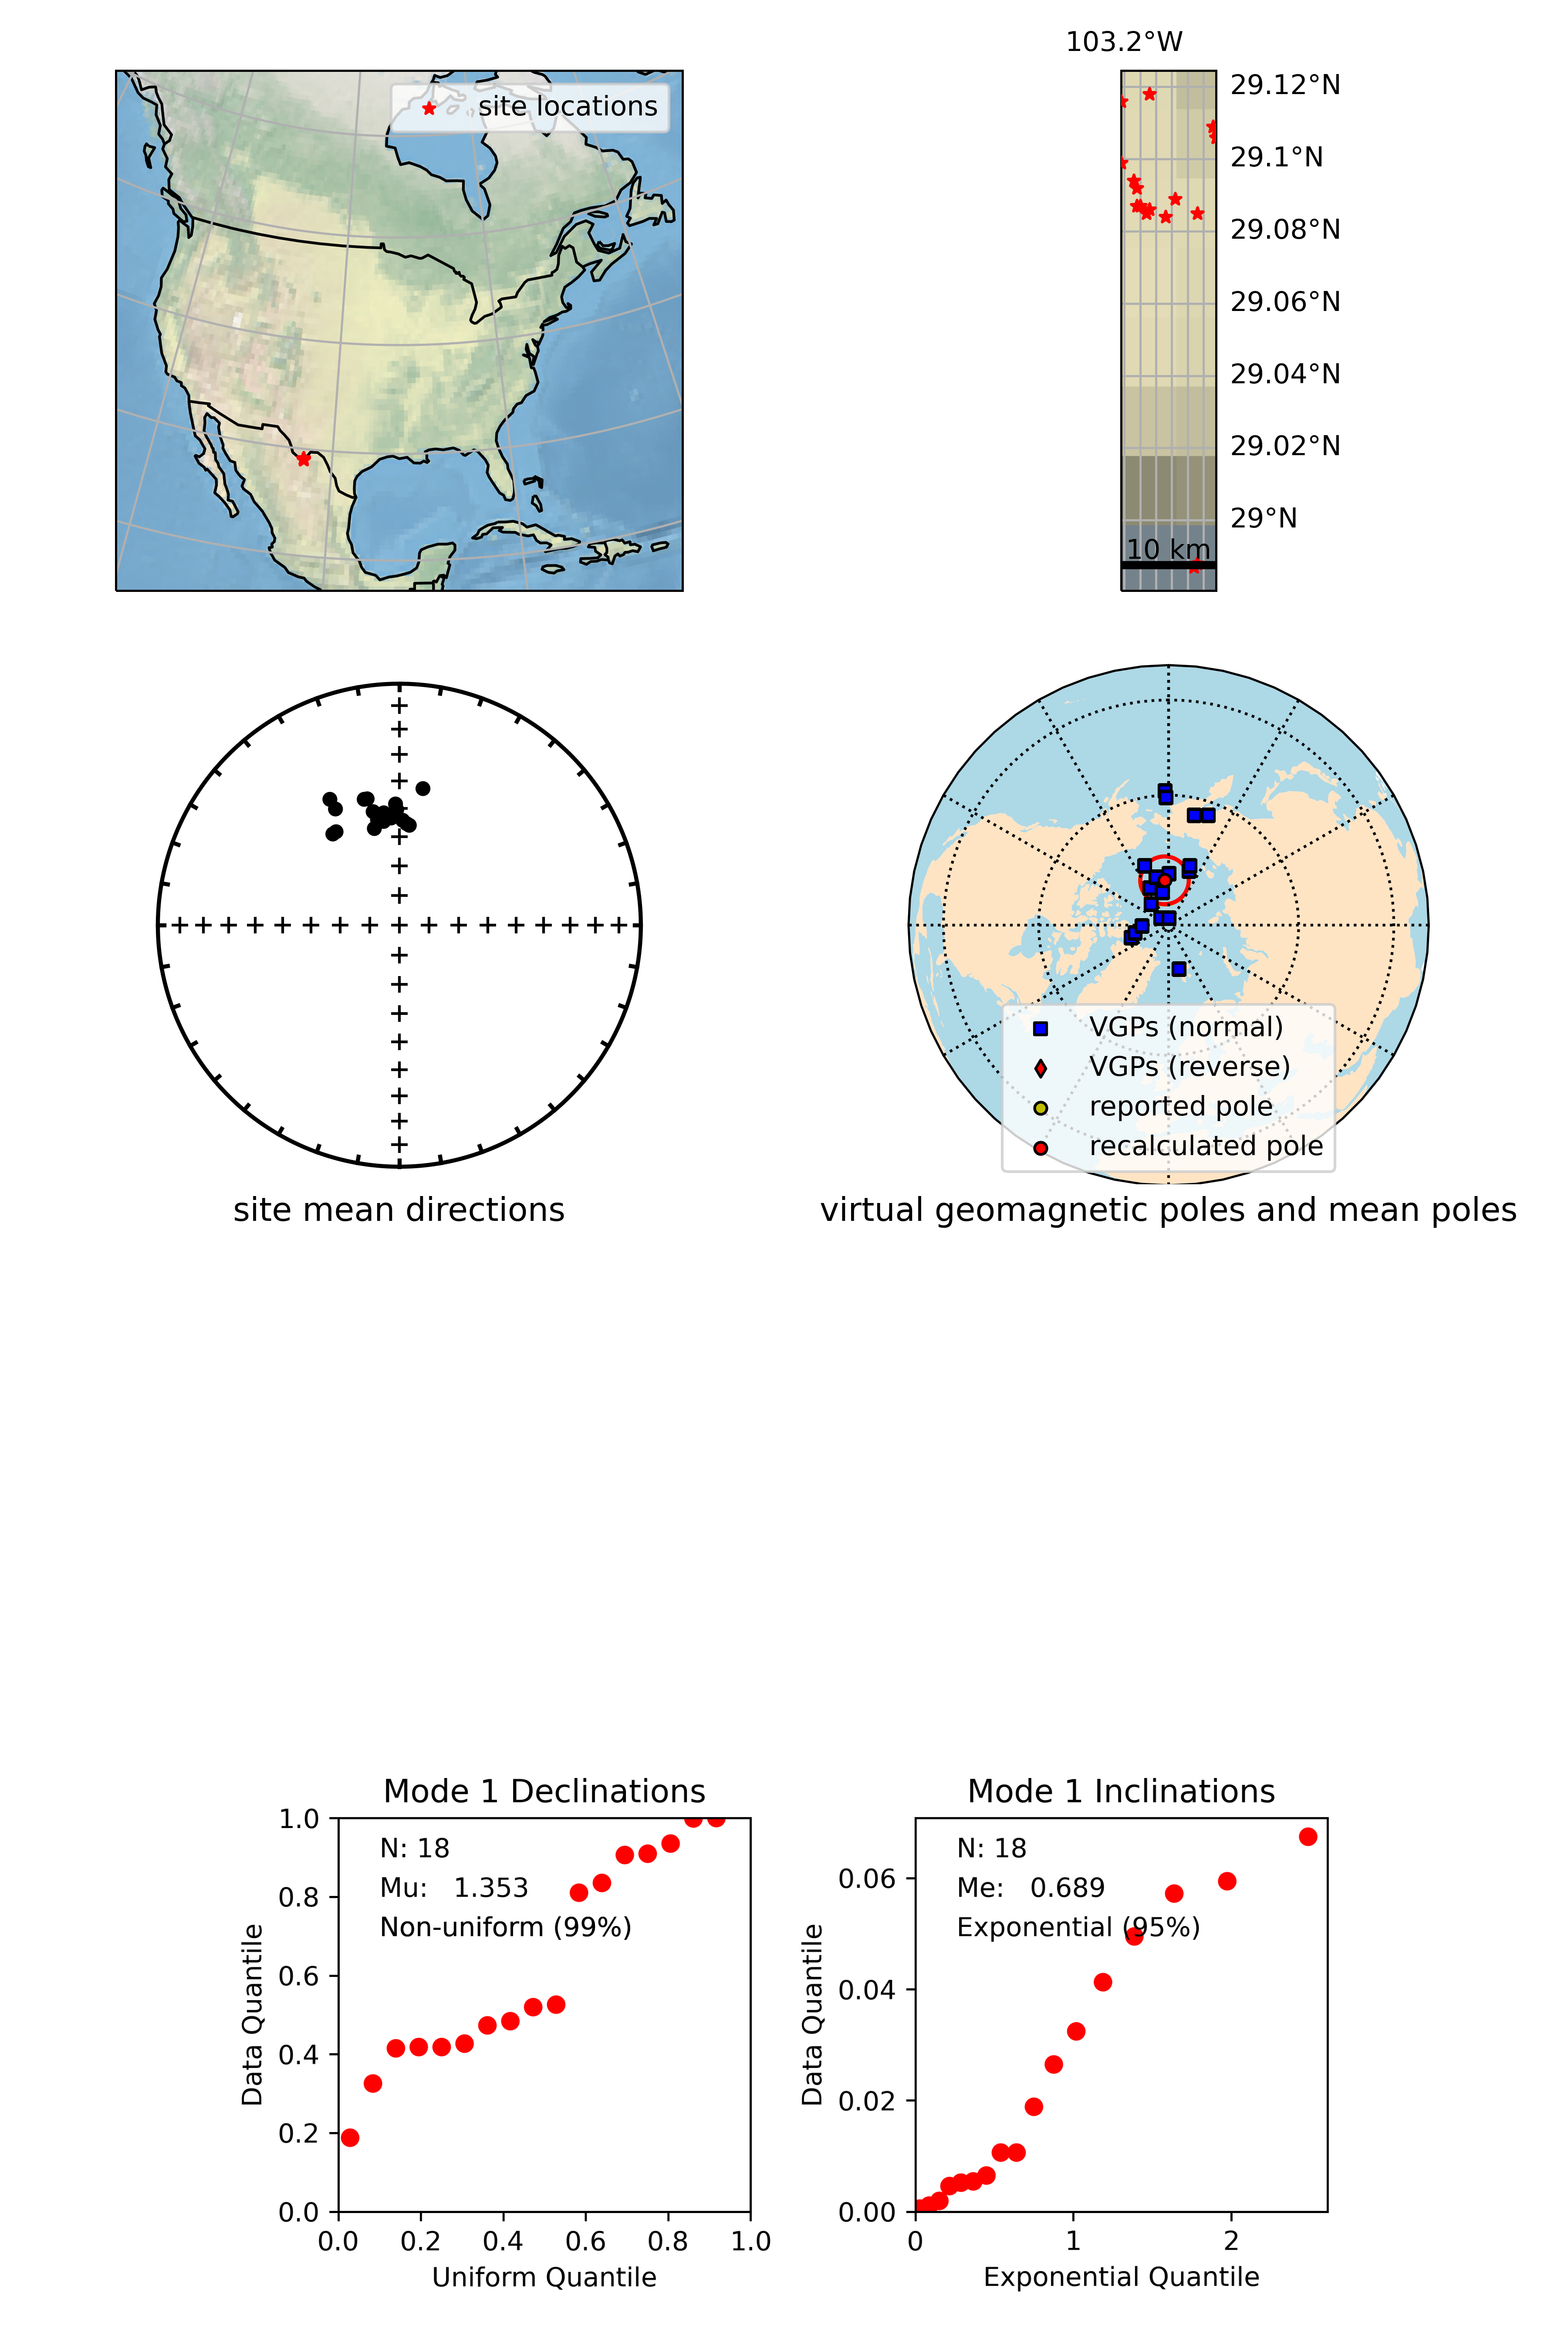
\includegraphics[width=5 in]{./27/1/pole_summary.png}
\caption{Summary of data from locality 27 (Mariscal Mtn intrusions) pole 1 (Harlan et al. (1995)).}
\end{figure}

\section{Mogollon-Datil volcanics}
\subsection{Pole 1}
\begin{tabular}{lllll}
\toprule
{} &   N &  Plat &   Plon &  A95 \\
\midrule
Reported mean pole                                 &  33 &  88.0 &  265.5 &  5.0 \\
Mean pole (calculated from VGPs)                   &  33 &  87.9 &  270.8 &  5.1 \\
Mean pole (calculated from transformed directions) &  33 &  87.9 &  270.6 &  5.1 \\
\bottomrule
\end{tabular}

\begin{tabular}{ll}
\toprule
{} &                                                          result \\
\midrule
Bootstrap reversal test  &                                                            Pass \\
Parametric reversal test &  Pass (angle 3.1º below 11.5º critical angle); C classification \\
Bayesian reversal test   &                                   Common mean: positive support \\
Fisher Q-Q test          &                             Consistent with Fisher distribution \\
\bottomrule
\end{tabular}

\begin{figure}[H]
\centering
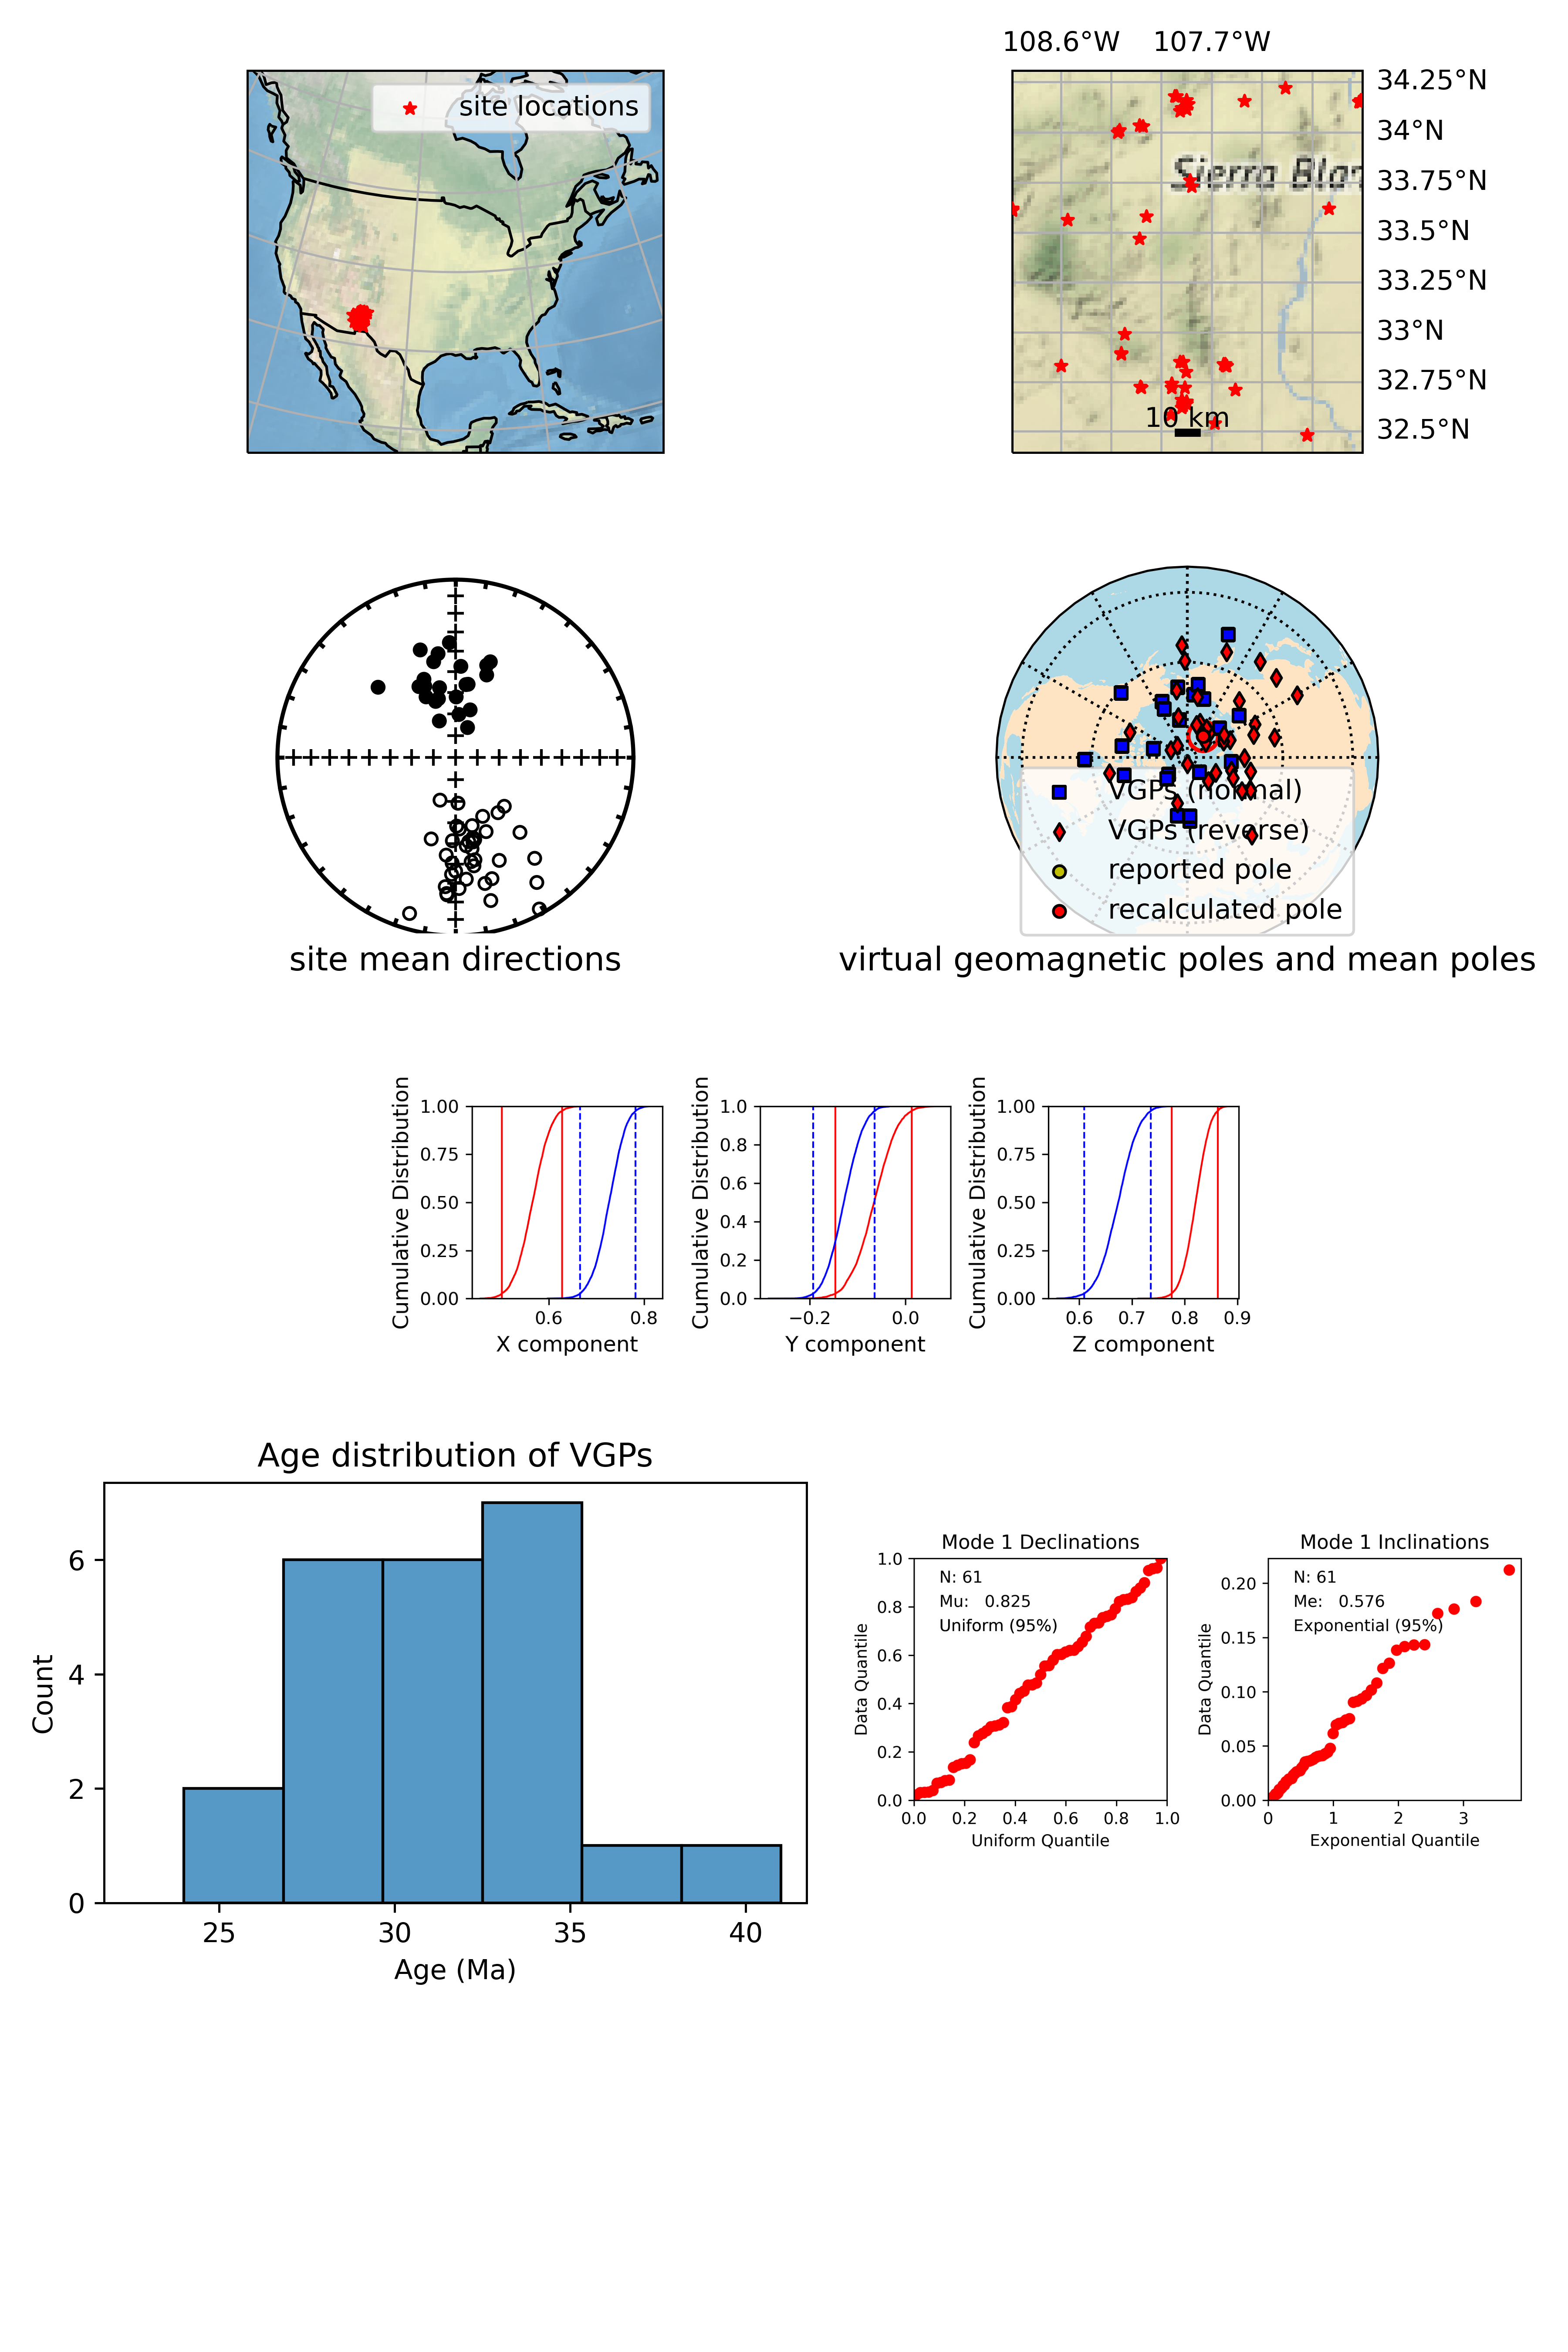
\includegraphics[width=5 in]{./28/1/pole_summary.png}
\caption{Summary of data from locality 28 (Mogollon-Datil volcanics) pole 1 (Diehl et al. (1988)).}
\end{figure}

\subsection{Pole 2}
\begin{tabular}{lllll}
\toprule
{} &   N &  Plat &   Plon &  A95 \\
\midrule
Reported mean pole                                 &  33 &  88.0 &  265.5 &  5.0 \\
Mean pole (calculated from VGPs)                   &  33 &  87.9 &  270.8 &  5.1 \\
Mean pole (calculated from transformed directions) &  33 &  87.9 &  270.6 &  5.1 \\
\bottomrule
\end{tabular}

\begin{tabular}{ll}
\toprule
{} &                                                          result \\
\midrule
Bootstrap reversal test  &                                                            Pass \\
Parametric reversal test &  Pass (angle 3.1º below 11.5º critical angle); C classification \\
Bayesian reversal test   &                                   Common mean: positive support \\
Fisher Q-Q test          &                             Consistent with Fisher distribution \\
\bottomrule
\end{tabular}

\begin{figure}[H]
\centering
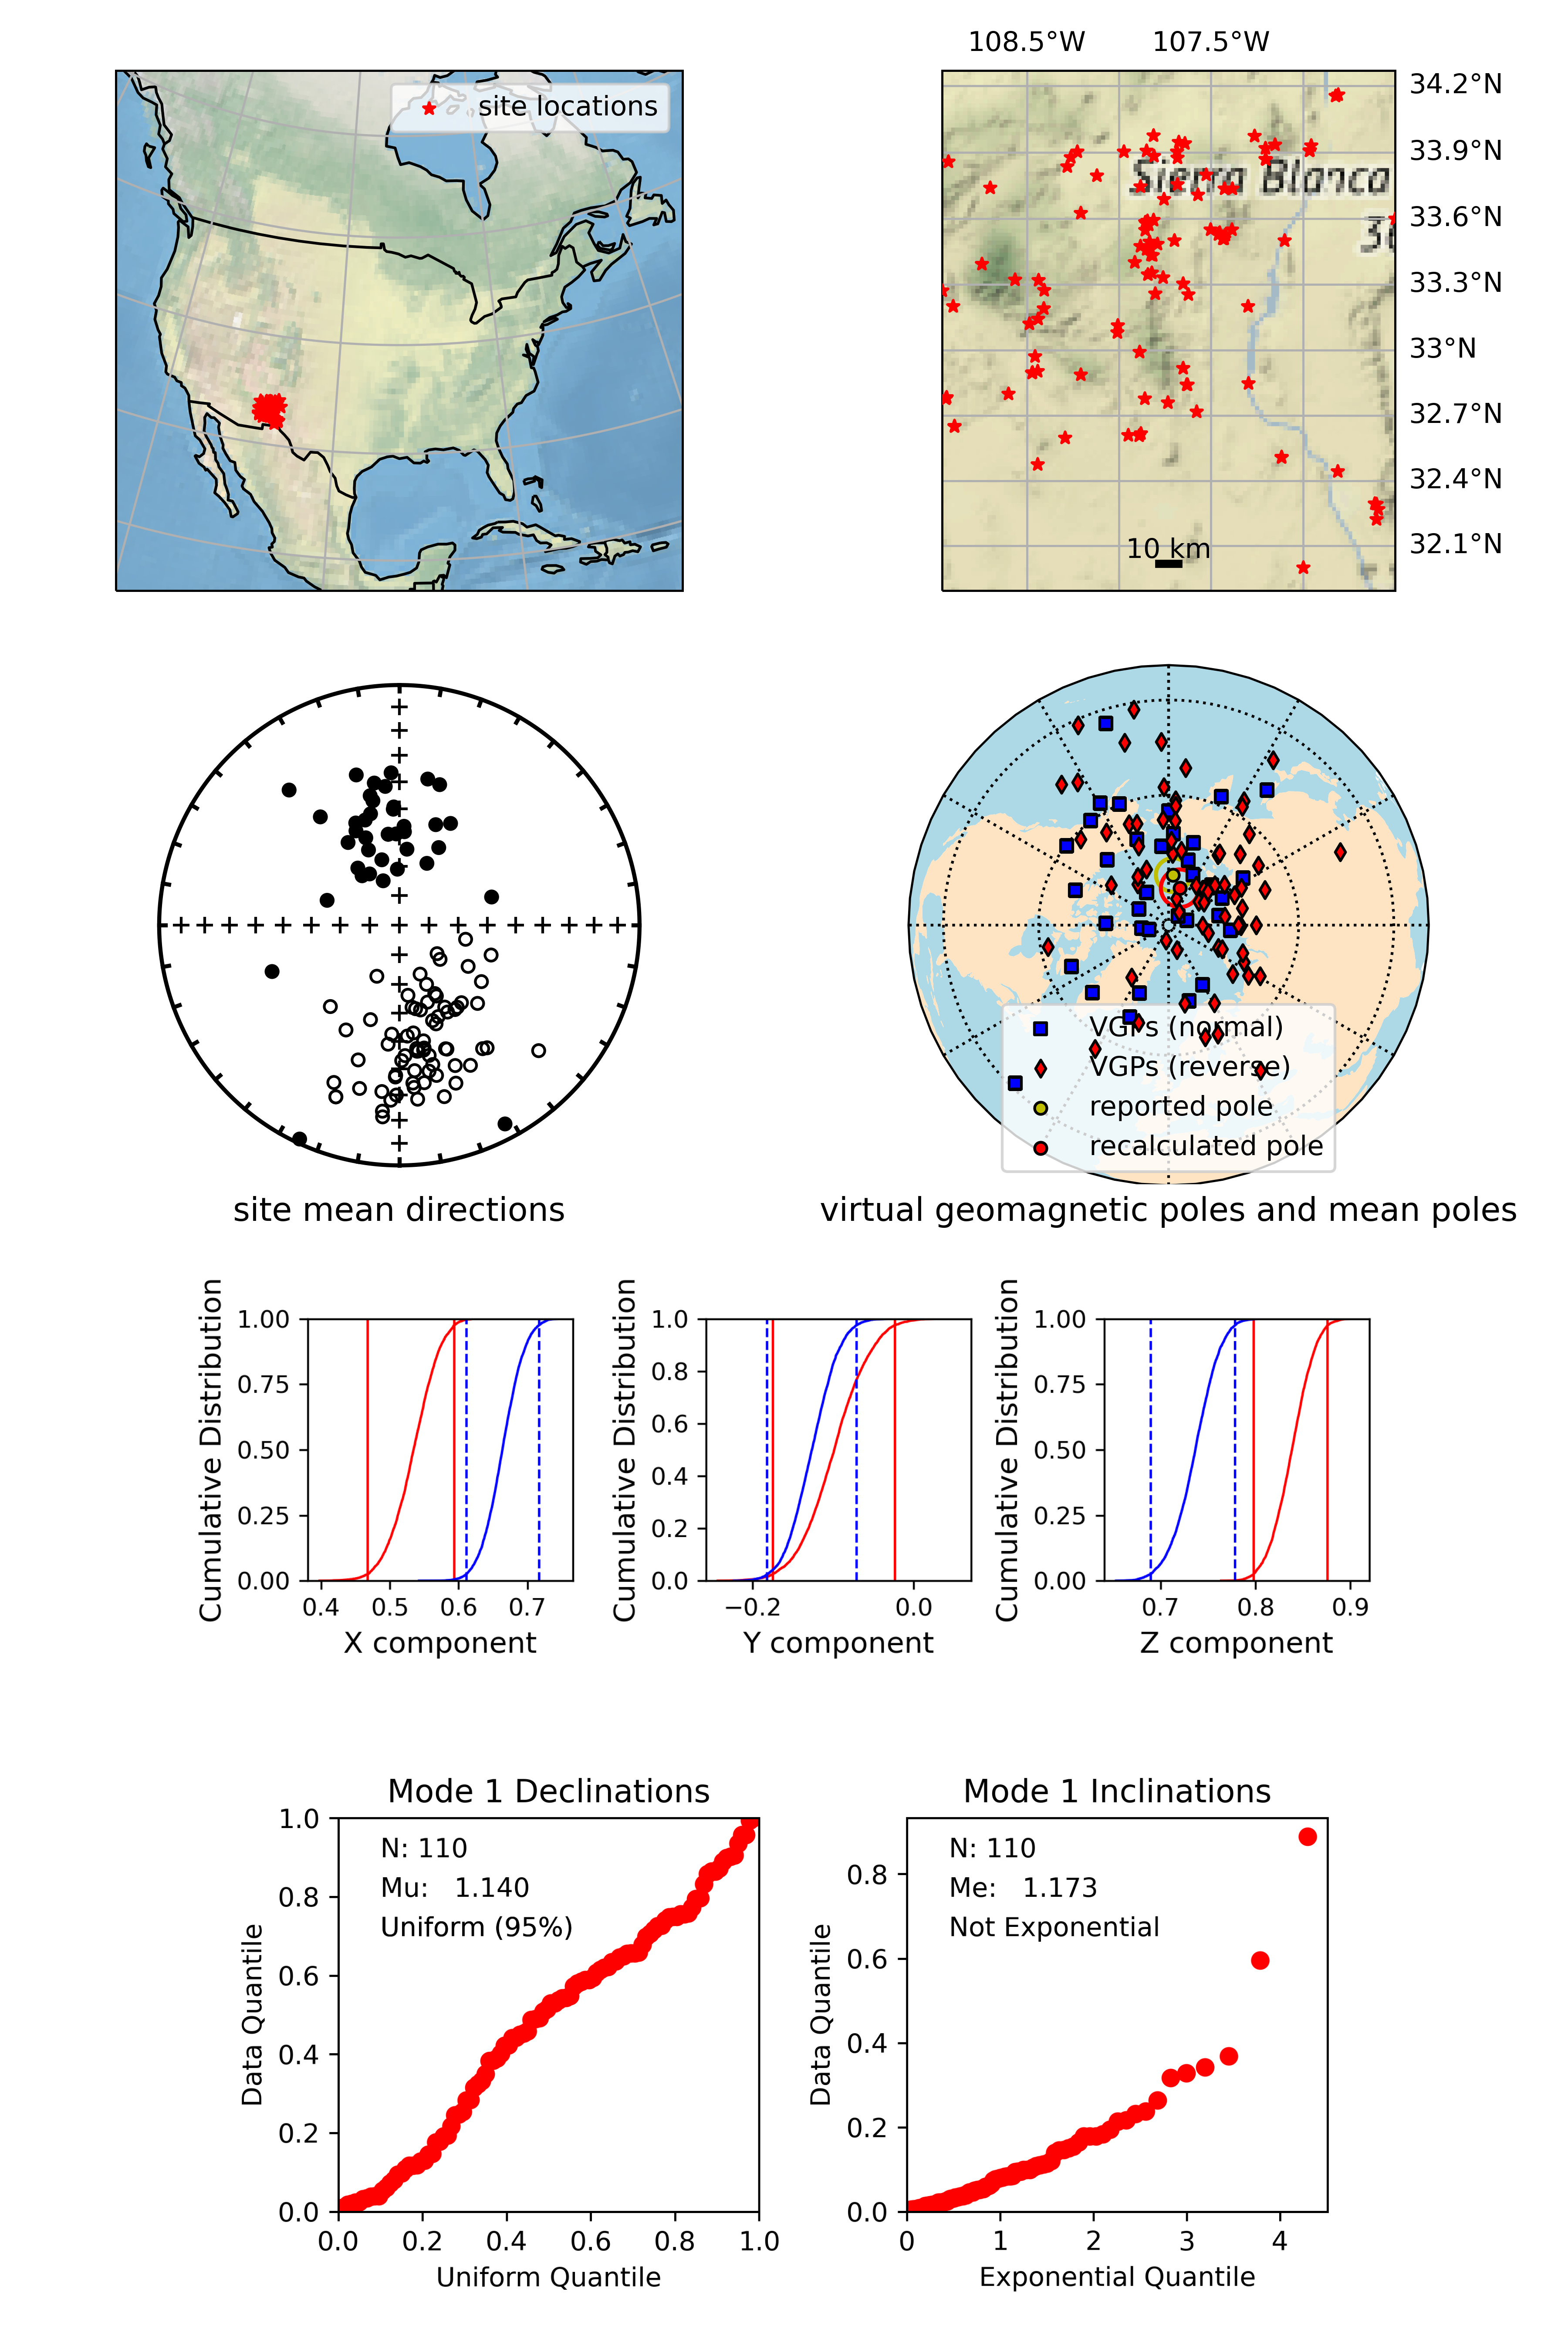
\includegraphics[width=5 in]{./28/2/pole_summary.png}
\caption{Summary of data from locality 28 (Mogollon-Datil volcanics) pole 2 (McIntosh (1991)).}
\end{figure}

\section{Monterey intrusions}
\subsection{Pole 1}
\begin{tabular}{lllll}
\toprule
{} &   N &  Plat &   Plon &  A95 \\
\midrule
Reported mean pole                                 &  33 &  88.0 &  265.5 &  5.0 \\
Mean pole (calculated from VGPs)                   &  33 &  87.9 &  270.8 &  5.1 \\
Mean pole (calculated from transformed directions) &  33 &  87.9 &  270.6 &  5.1 \\
\bottomrule
\end{tabular}

\begin{tabular}{ll}
\toprule
{} &                                                          result \\
\midrule
Bootstrap reversal test  &                                                            Pass \\
Parametric reversal test &  Pass (angle 3.1º below 11.5º critical angle); C classification \\
Bayesian reversal test   &                                   Common mean: positive support \\
Fisher Q-Q test          &                             Consistent with Fisher distribution \\
\bottomrule
\end{tabular}

\begin{figure}[H]
\centering
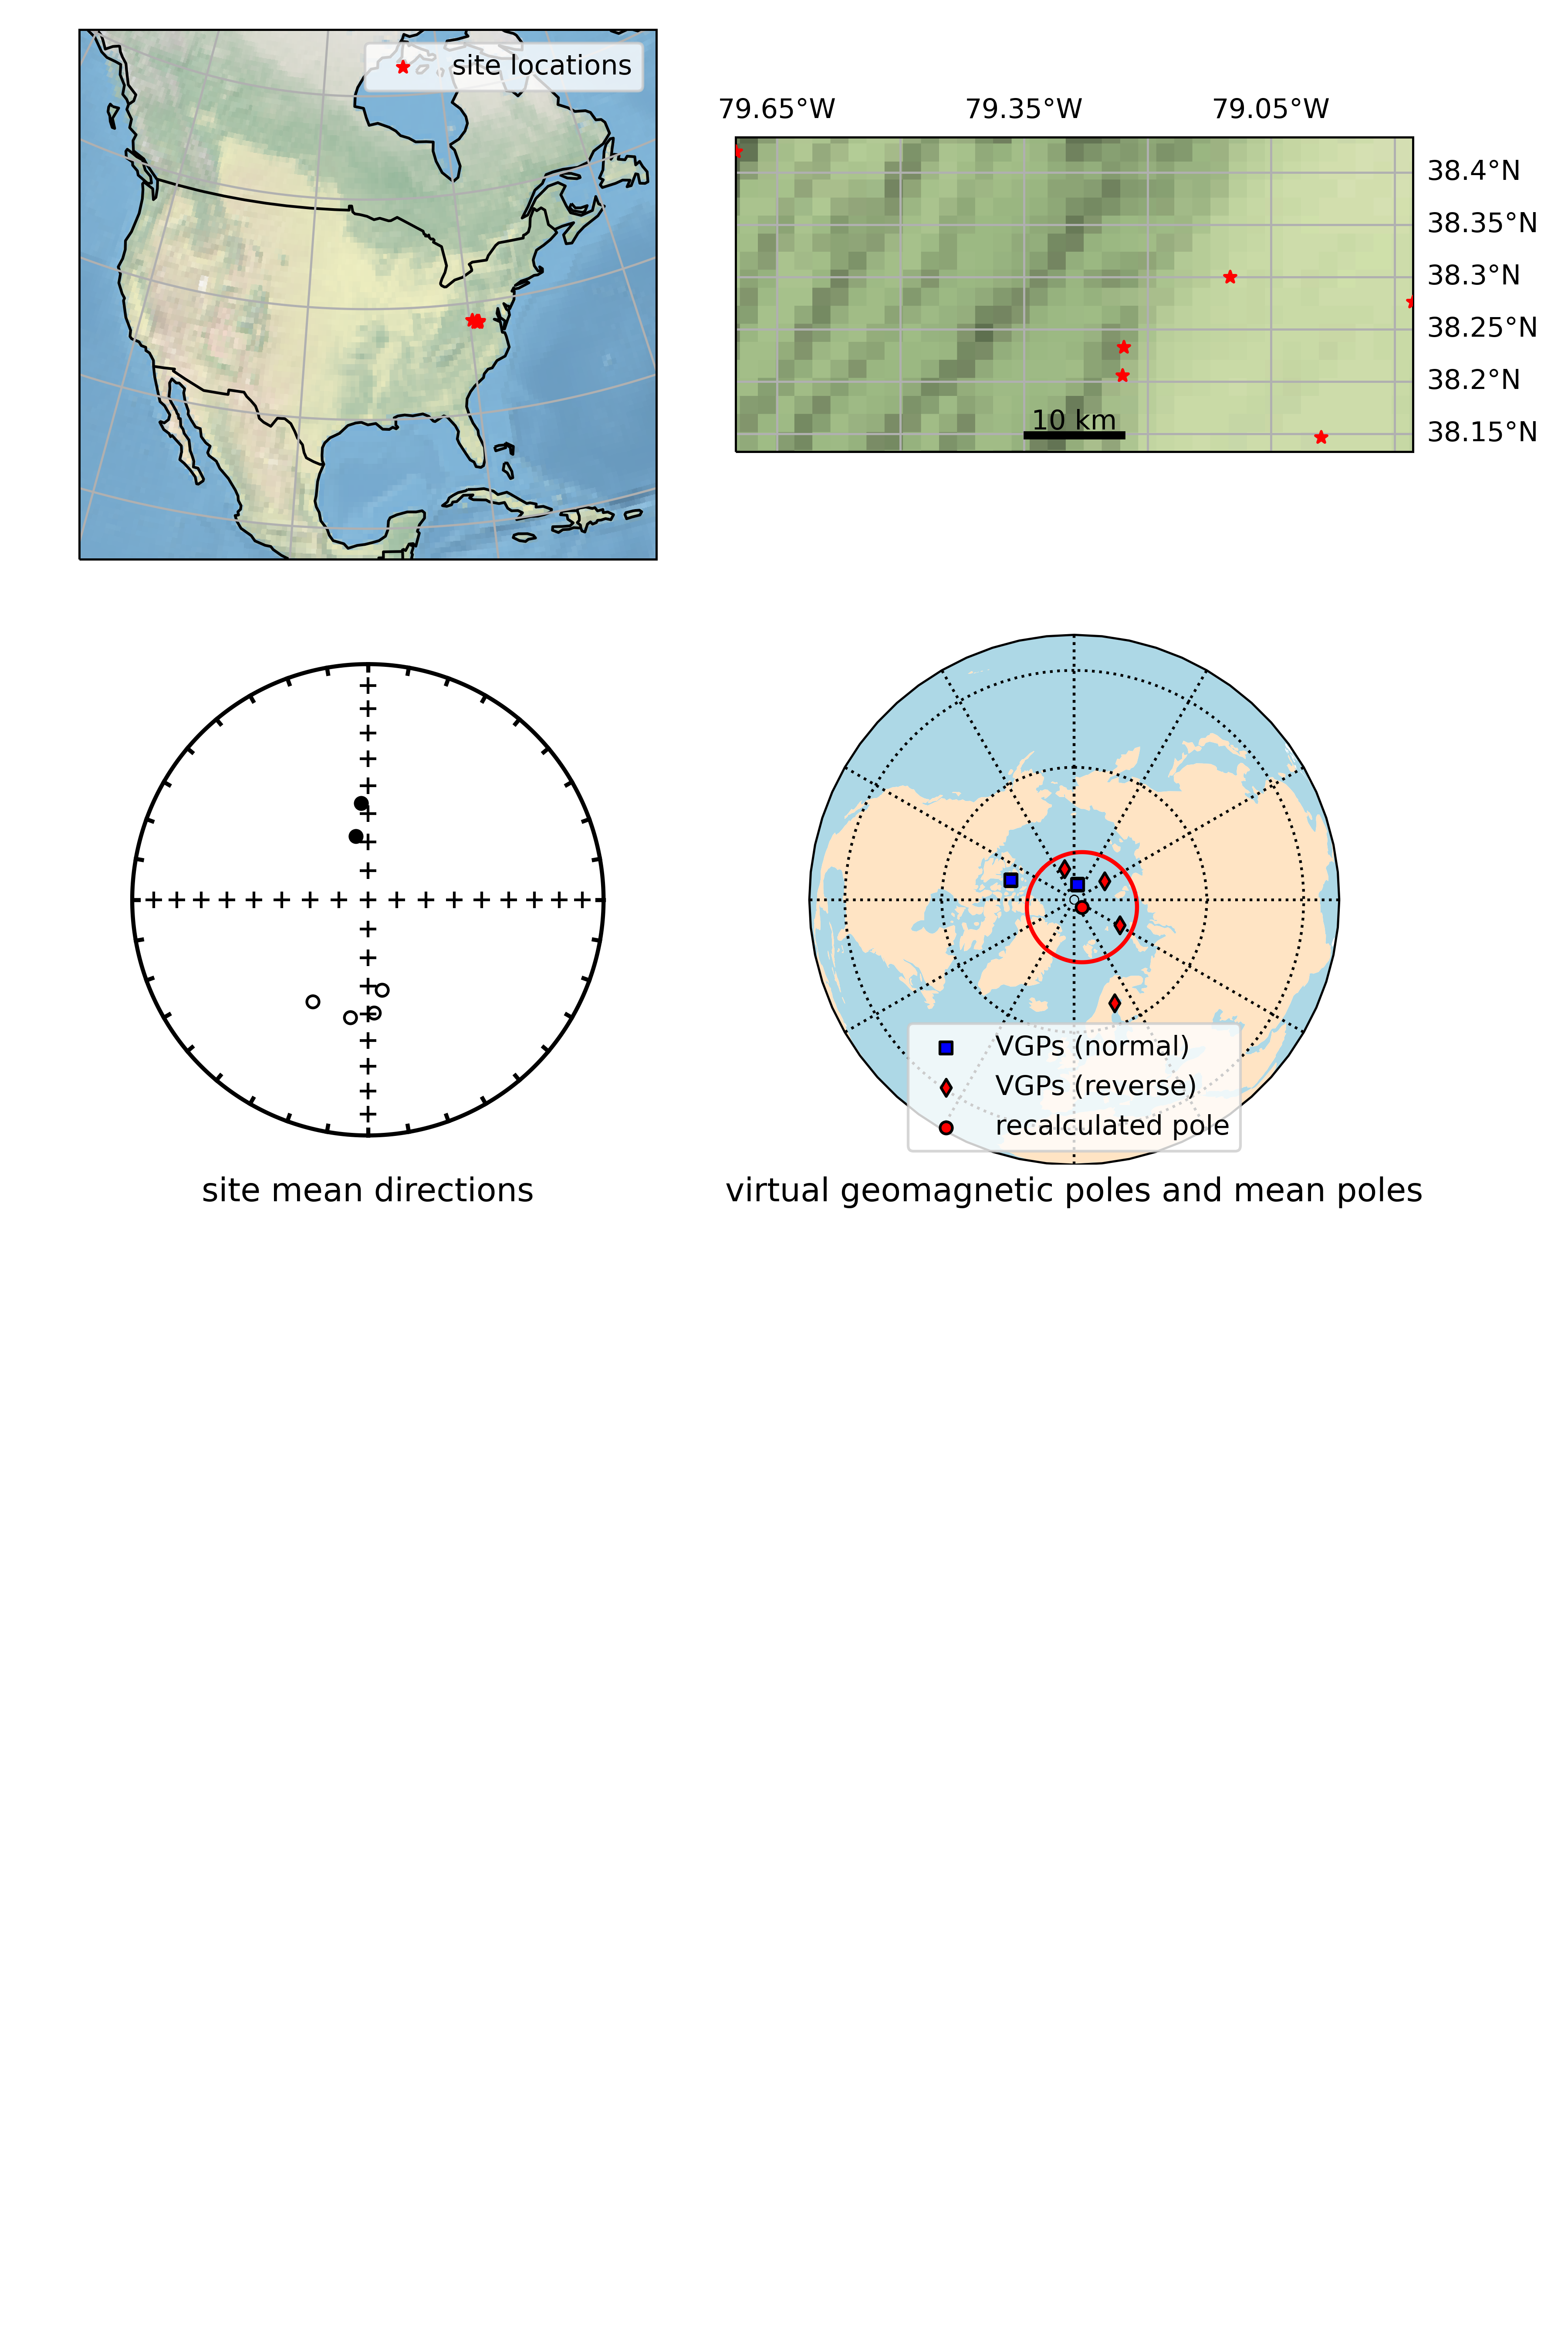
\includegraphics[width=5 in]{./29/1/pole_summary.png}
\caption{Summary of data from locality 29 (Monterey intrusions) pole 1 (Løvlie and Opdyke (1974)).}
\end{figure}

\subsection{Pole 2}
\begin{tabular}{lllll}
\toprule
{} &   N &  Plat &   Plon &  A95 \\
\midrule
Reported mean pole                                 &  33 &  88.0 &  265.5 &  5.0 \\
Mean pole (calculated from VGPs)                   &  33 &  87.9 &  270.8 &  5.1 \\
Mean pole (calculated from transformed directions) &  33 &  87.9 &  270.6 &  5.1 \\
\bottomrule
\end{tabular}

\begin{tabular}{ll}
\toprule
{} &                                                          result \\
\midrule
Bootstrap reversal test  &                                                            Pass \\
Parametric reversal test &  Pass (angle 3.1º below 11.5º critical angle); C classification \\
Bayesian reversal test   &                                   Common mean: positive support \\
Fisher Q-Q test          &                             Consistent with Fisher distribution \\
\bottomrule
\end{tabular}

\begin{figure}[H]
\centering
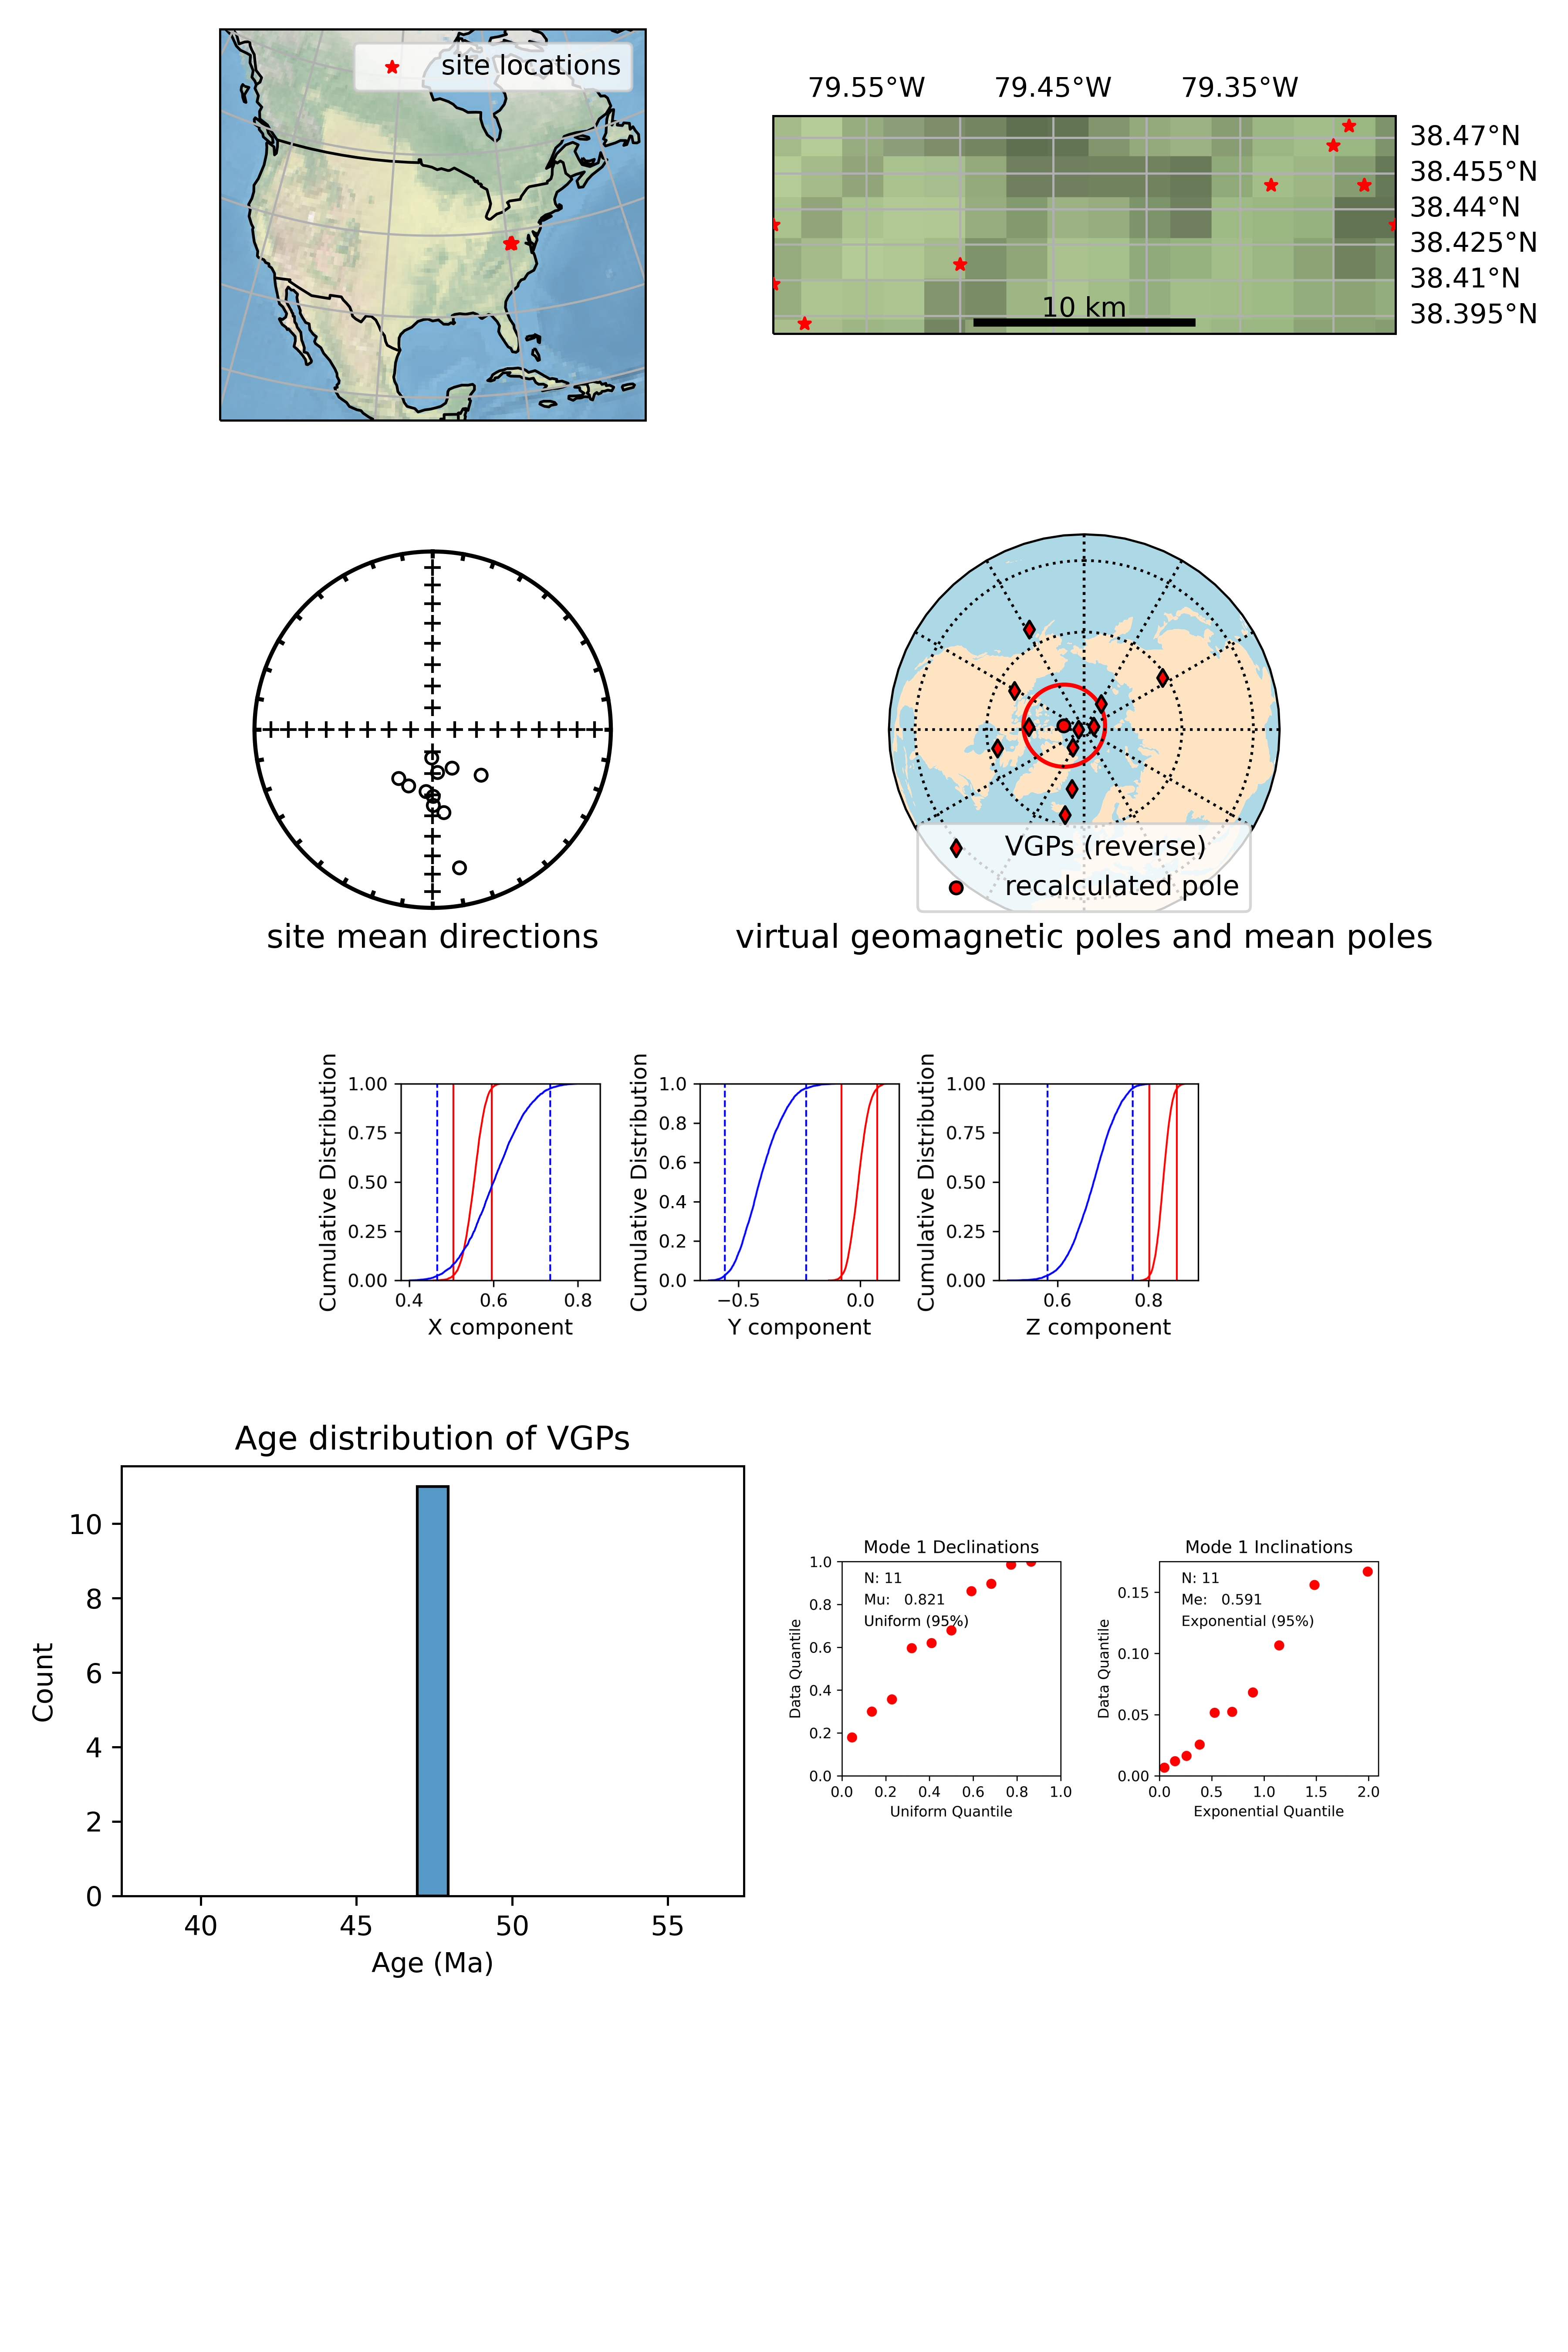
\includegraphics[width=5 in]{./29/2/pole_summary.png}
\caption{Summary of data from locality 29 (Monterey intrusions) pole 2 (Ressetar and Martin (1980)).}
\end{figure}

\section{Latir volcanic field}
\subsection{Pole 1}
\begin{tabular}{lllll}
\toprule
{} &   N &  Plat &   Plon &  A95 \\
\midrule
Reported mean pole                                 &  33 &  88.0 &  265.5 &  5.0 \\
Mean pole (calculated from VGPs)                   &  33 &  87.9 &  270.8 &  5.1 \\
Mean pole (calculated from transformed directions) &  33 &  87.9 &  270.6 &  5.1 \\
\bottomrule
\end{tabular}

\begin{tabular}{ll}
\toprule
{} &                                                          result \\
\midrule
Bootstrap reversal test  &                                                            Pass \\
Parametric reversal test &  Pass (angle 3.1º below 11.5º critical angle); C classification \\
Bayesian reversal test   &                                   Common mean: positive support \\
Fisher Q-Q test          &                             Consistent with Fisher distribution \\
\bottomrule
\end{tabular}

\begin{figure}[H]
\centering
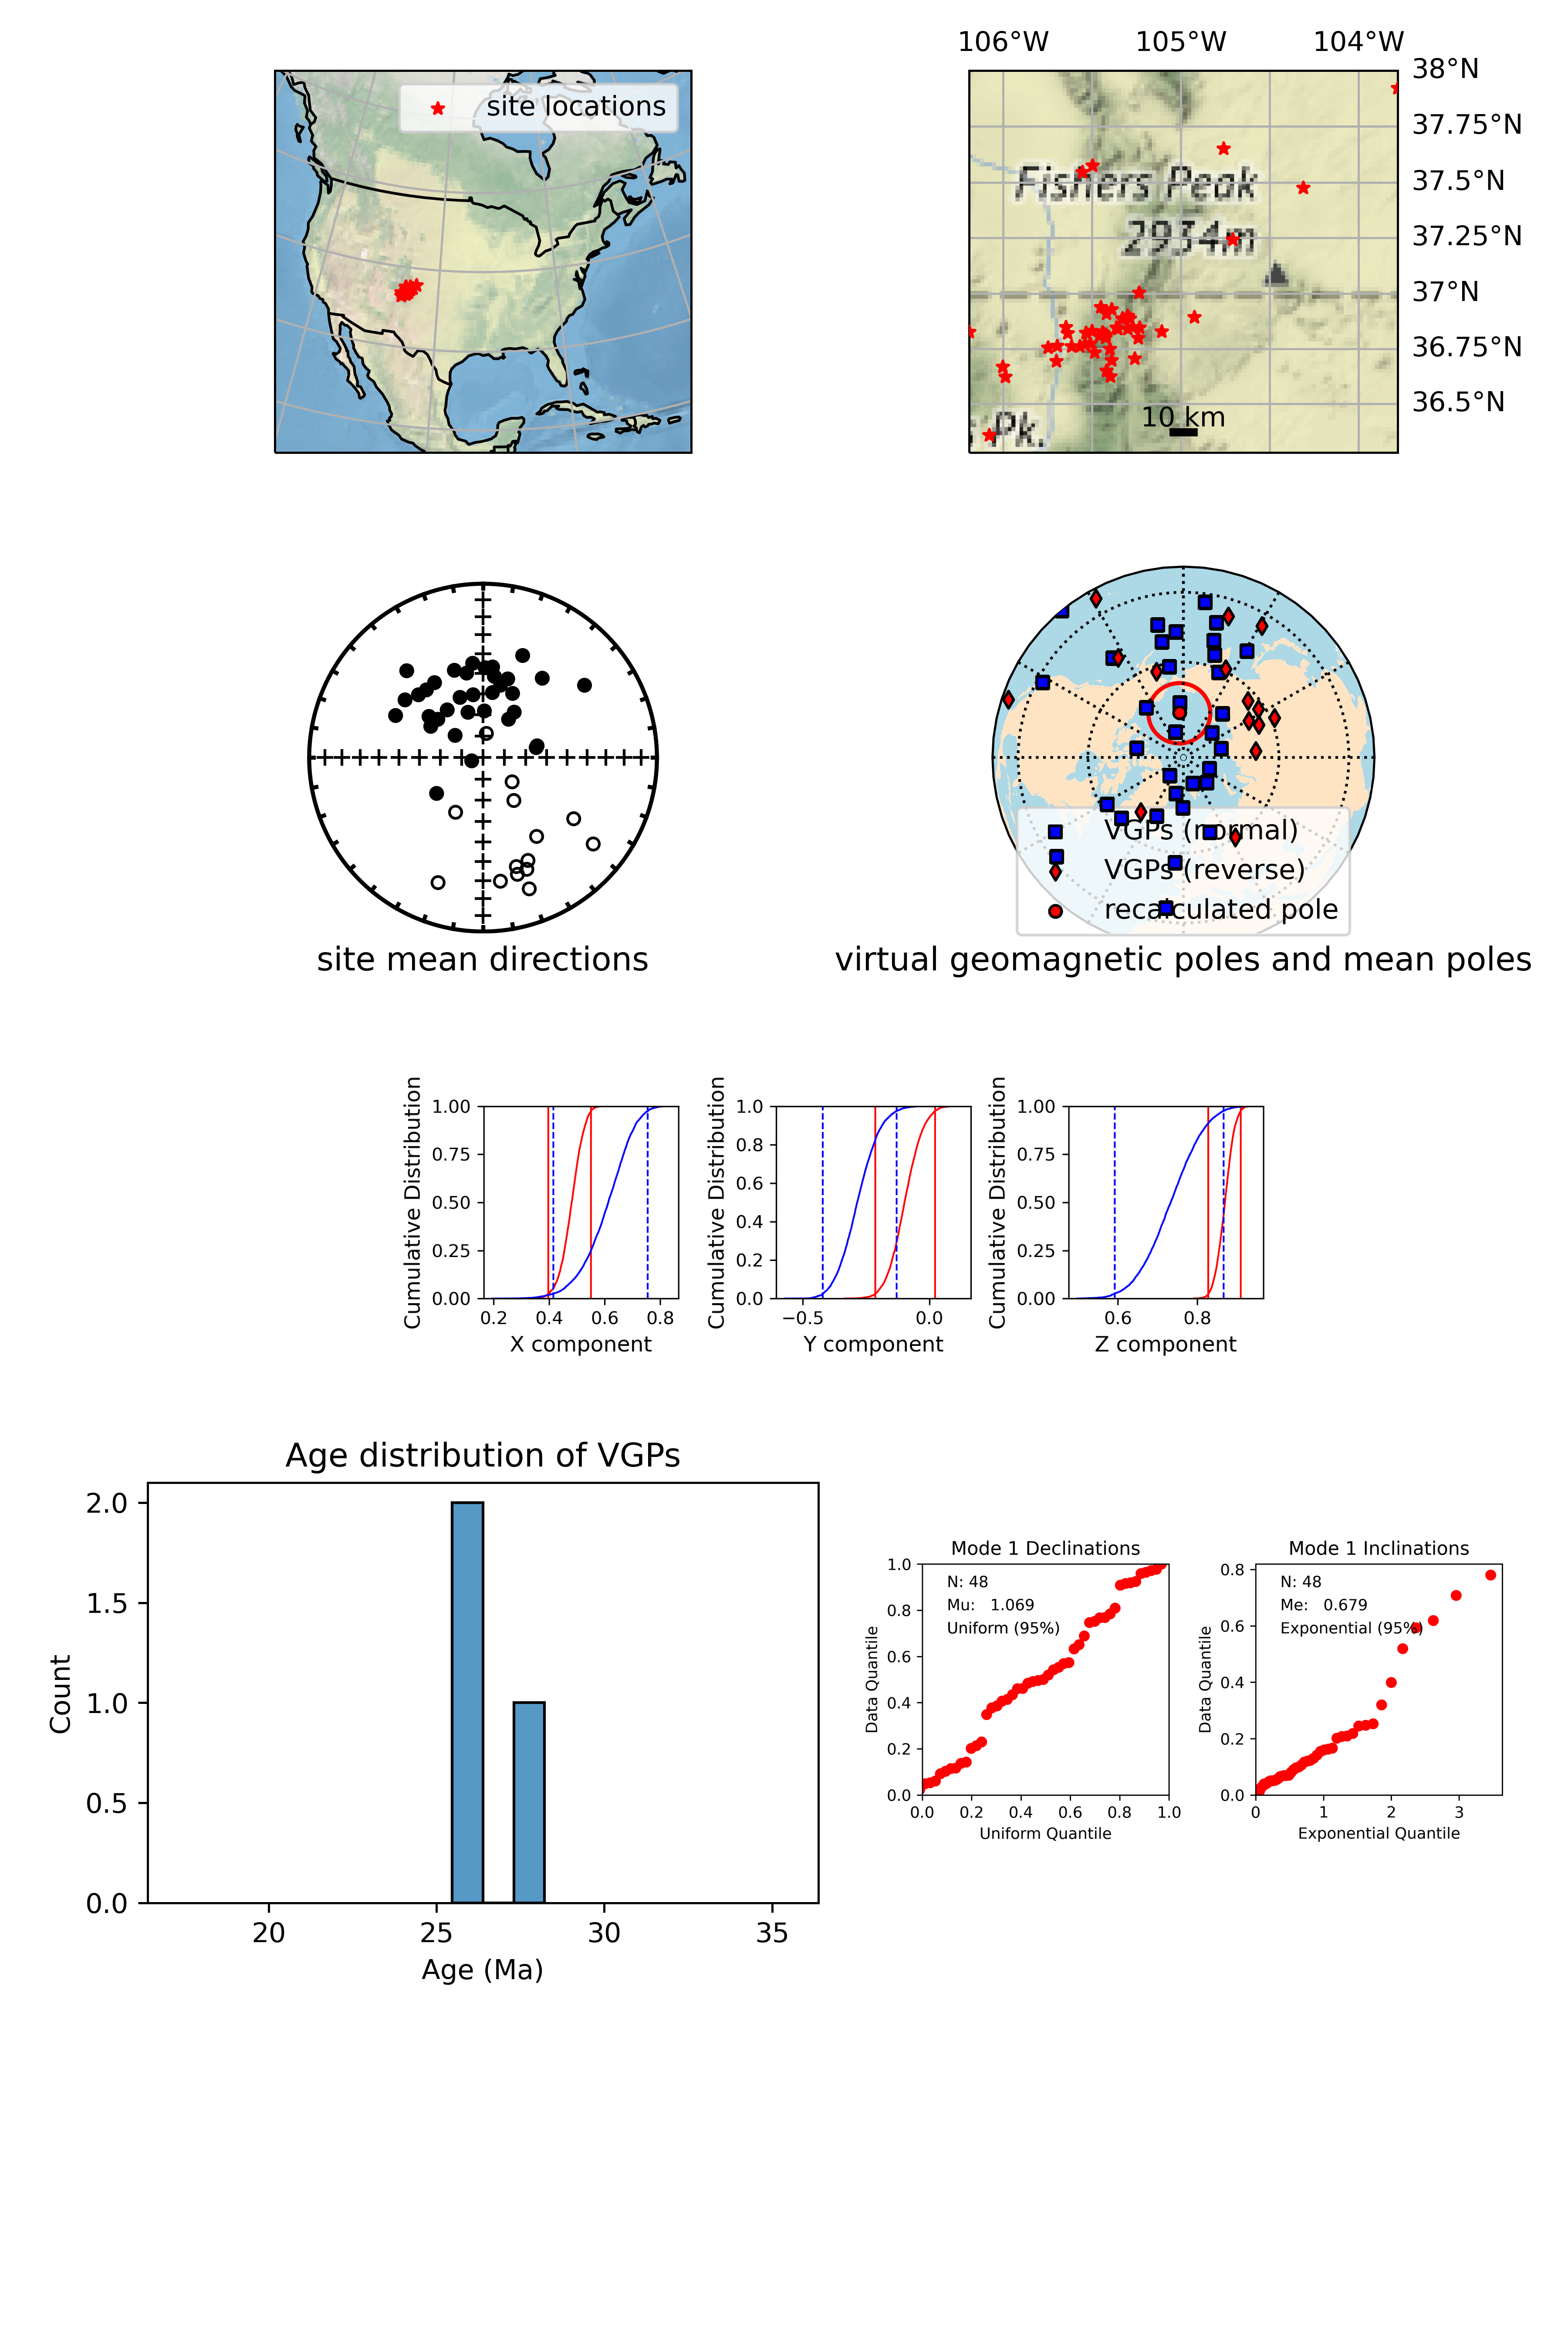
\includegraphics[width=5 in]{./30/1/pole_summary.png}
\caption{Summary of data from locality 30 (Latir volcanic field) pole 1 (Hagstrum and Lipman (1986)).}
\end{figure}

\subsection{Pole 2}
\begin{tabular}{lllll}
\toprule
{} &   N &  Plat &   Plon &  A95 \\
\midrule
Reported mean pole                                 &  33 &  88.0 &  265.5 &  5.0 \\
Mean pole (calculated from VGPs)                   &  33 &  87.9 &  270.8 &  5.1 \\
Mean pole (calculated from transformed directions) &  33 &  87.9 &  270.6 &  5.1 \\
\bottomrule
\end{tabular}

\begin{tabular}{ll}
\toprule
{} &                                                          result \\
\midrule
Bootstrap reversal test  &                                                            Pass \\
Parametric reversal test &  Pass (angle 3.1º below 11.5º critical angle); C classification \\
Bayesian reversal test   &                                   Common mean: positive support \\
Fisher Q-Q test          &                             Consistent with Fisher distribution \\
\bottomrule
\end{tabular}

\begin{figure}[H]
\centering
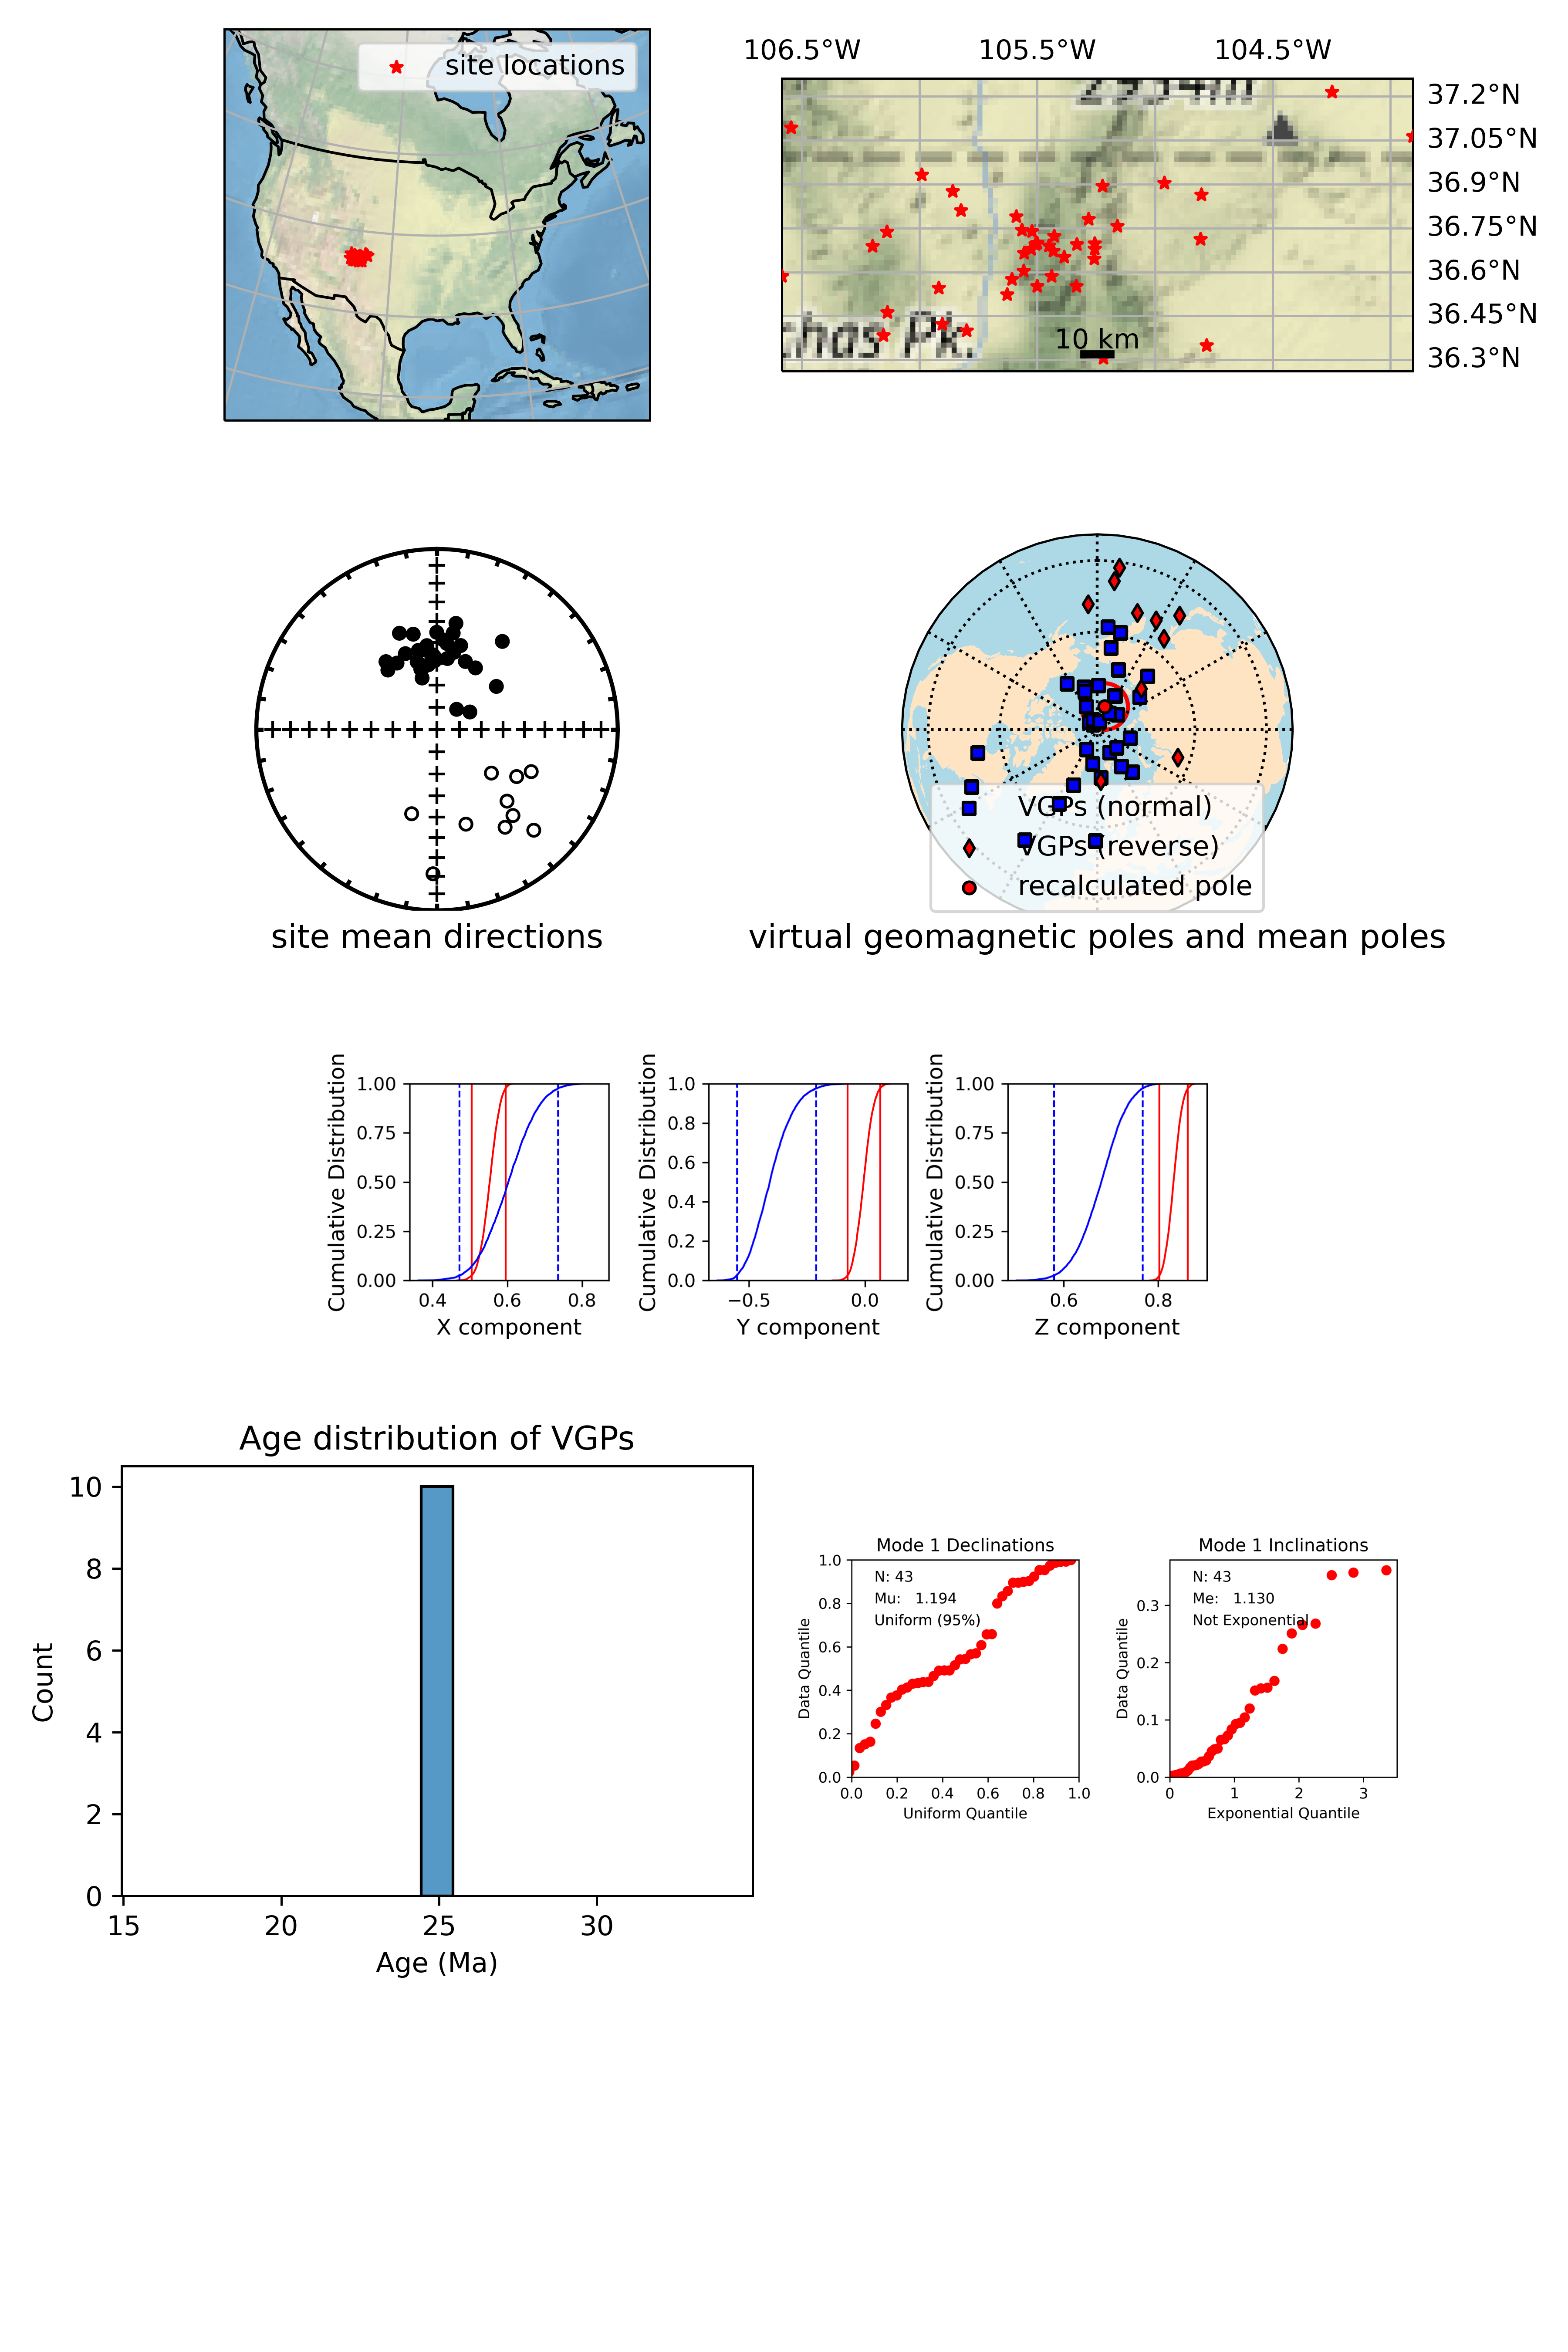
\includegraphics[width=5 in]{./30/2/pole_summary.png}
\caption{Summary of data from locality 30 (Latir volcanic field) pole 2 (Hagstrum and Lipman (1986)).}
\end{figure}

\end{document}

